% =================================================================
% AFRAS-FL / MDPI AI - SEPARATE EDITORIAL CONVERSION DRAFT
% SOURCE: paper/main.tex. Scientific text, tables, equations, figure
% references, results and citations in the body are retained verbatim.
% THIS IS NOT A VERIFIED EXPERIMENT OR SUBMISSION-READY MANUSCRIPT.
% Never substitute new strict-Stage4 v2 results for historical values.
%
% The publisher's current Definitions/ directory is intentionally NOT
% committed here; obtain it from https://www.mdpi.com/authors/latex .
% Compile with CWD paper/mdpi_ai/; ../figures and ../references.bib are
% reused unchanged. See docs/MDPI_AI_CONVERSION_README.md.
% =================================================================
\documentclass[ai,article,submit,moreauthors,pdftex]{Definitions/mdpi}

% Only additional packages that occur in the original IEEE source.
% MDPI's current class already provides graphicx, booktabs, amsmath,
% amsthm, hyperref, natbib, caption, xcolor, TikZ and soul.
\usepackage{placeins}
\usepackage{mathrsfs}
\usepackage{amsfonts}
\usepackage{textcomp}
\usepackage{algorithm}
\usepackage{algorithmicx}
\usepackage{algpseudocode}
\usepackage{listings}
\usepackage{subcaption}
\usepackage{tabularx}
\usepackage{makecell}
\usetikzlibrary{arrows.meta,positioning,shapes.geometric,fit,backgrounds,calc,shadows}

% MDPI has capitalized mathematical environments; map the lowercase
% environment names already used in the source without rewriting proofs.
\newenvironment{theorem}{\begin{Theorem}}{\end{Theorem}}
\newenvironment{proposition}{\begin{Proposition}}{\end{Proposition}}
\newenvironment{example}{\begin{Example}}{\end{Example}}
\newenvironment{remark}{\begin{Remark}}{\end{Remark}}
\newenvironment{definition}{\begin{Definition}}{\end{Definition}}

% Clean reading/submission styling: reviewer-added \\rev text prints in
% ordinary black. Text marked \\strk as deleted prints nothing in the PDF
% (but remains in the TeX source for provenance/reviewer comparison).
% No experimental result, number or scientific wording was changed.
\newcommand{\rev}[1]{#1}
\newcommand{\strk}[1]{}

% Relative paths are evaluated from the LaTeX working directory.
\graphicspath{{../figures/}}

% MDPI class requires these typesetting fields in the publisher package.
% ALL numbers are TEMPLATE PLACEHOLDERS, not a real journal volume, issue,
% article number, publication acceptance, copyright clearance, or DOI.
% Do not present them as published bibliographic facts.
\pubvolume{1}
\issuenum{1}
\articlenumber{0}
\pubyear{2026}
\copyrightyear{2026}
\datereceived{ }
\daterevised{ }
\dateaccepted{ }
\datepublished{ }

% MDPI FRONT MATTER: author details are transcribed from the preserved
% IEEE original only; corresponding authorship and affiliations still
% require explicit confirmation by all authors before submission.
\firstpage{1}
\Title{Fuzzy-Augmented Reward Shaping for Multi-Objective Deep Reinforcement Learning in Federated SDN-IoT Intrusion Detection}
\TitleCitation{Fuzzy-Augmented Reward Shaping for Federated SDN-IoT Intrusion Detection}

\newcommand{\orcidauthorA}{0000-0003-1360-130X}
\newcommand{\orcidauthorB}{0000-0001-6193-3240}
\newcommand{\orcidauthorC}{0000-0002-1019-4123}

\Author{Ali Hussein Fadel $^{1,}$*\orcidA{}, Jaber Karimpour $^{1}$\orcidB{} and Zolfaghar Salmanian Kozehkonan $^{2}$\orcidC{}}
\AuthorNames{Ali Hussein Fadel, Jaber Karimpour and Zolfaghar Salmanian Kozehkonan}
\AuthorCitation{Fadel, A.H.; Karimpour, J.; Kozehkonan, Z.S.}
\address{%
$^{1}$ \quad Department of Computer Science, Faculty of Mathematics, Statistics, and Computer Science, University of Tabriz, Tabriz, Iran; ali\_hussein\_fadel@uodiyala.edu.iq (A.H.F.); karimpour@tabrizu.ac.ir (J.K.)\\
$^{2}$ \quad Department of Computer Engineering, Faculty of Electrical and Computer Engineering, University of Tabriz, Tabriz, Iran; salmanian@tabrizu.ac.ir (Z.S.K.)}
\corres{Correspondence: ali\_hussein\_fadel@uodiyala.edu.iq (A.H.F.)}

% Abstract is inherited verbatim, including historical unverified metrics.
\abstract{
Software-defined IoT (SDN-IoT) networks demand intrusion detection
systems that learn online from heterogeneous edge data without
centralising raw flows. Federated deep reinforcement learning (DRL)
satisfies this constraint, yet agents trained under non-IID client
distributions suffer from unstable convergence, brittle
generalisation, and opaque decision behaviour. The culprit is largely
the reward function: scalar single-objective rewards collapse the
trade-offs between detection accuracy, latency, and false-alarm cost,
and they provide no inductive bias when client distributions diverge.
We propose MOSAR, a Multi-Objective Security-Aware Reward that
decomposes agent feedback into five interpretable components, together
with AFRAS-FL, an Adaptive Fuzzy Rule-Augmented Shaping pipeline that
\rev{mines IF--THEN fuzzy rules from a supervised label-partitioned grid over the top-variance features and converts them into a heuristic rule-agreement bonus (not a strict potential-based signal; see Sec.~\ref{sec:methods_theory}).} The combined reward
$R_{\text{total}} = R_{\text{MOSAR}} + \lambda R_{\text{fuzzy}} + \mu
R_{\text{link}}$ \rev{is motivated by the Ng et~al.\ potential-based shaping condition (recalled as a design reference in Proposition~\ref{prop:invariance}); we transparently discuss in Sec.~\ref{sec:methods_theory} why the released implementation of $R_{\text{fuzzy}}$ and $R_{\text{link}}$ does \emph{not} exactly satisfy this condition and therefore we do not claim exact policy invariance.} The full
pipeline is evaluated on two IoT benchmarks (CICIoT2023 and DIAD2024)
across a five-link SDN-IoT topology (Core, two Aggregation, two Edge)
\rev{with a role-based non-IID partition across the five topology links (see Sec.~\ref{sec:methods_data}),} and is compared against a
purpose-built federated multi-agent DQN baseline that shares the same
backbone, clients, and hyperparameters but uses neither MOSAR nor the
fuzzy shaping term. On CICIoT2023 the pipeline reaches a Mean Success
Rate (MSR) of $0.9990 \pm 0.0010$ at the fuzzy-augmented phase,
improves the FedAvg baseline by $+33.1$ percentage points
($p = 1.8 \times 10^{-15}$, Cohen's $d = 2.29$) and FedProx by
$+17.5$ percentage points ($p = 3.1 \times 10^{-12}$, $d = 1.84$),
and cuts the FedProx MSR standard deviation by a factor of $48$. On
the structurally adversarial DIAD2024 benchmark, the pipeline beats
the baseline on the Independent and FedAvg MSR variants ($+2.4$ and
$+8.9$ pp) and shrinks the FedProx false-positive rate from
$26.98\%$ to $0.18\%$ ($150\times$ reduction), \rev{a gain that is attained at the federated phase B3 (FedProx) before fuzzy augmentation is applied; the full pipeline (phase B4) has an FPR of $4.21\%$ on DIAD2024 and loses $5.5$ percentage points of MSR against B3, which we report honestly in Sec.~\ref{sec:r6_envelope} as an operational envelope of AFRAS-FL.} \rev{Similarly, the head-to-head gains reported against FedAvg and FedProx correspond to the full pipeline that jointly benefits from MOSAR's multi-objective decomposition, from the coordination term, and from AFRAS-FL; a controlled per-component ablation ($R_{\text{MOSAR}}$ alone, $R_{\text{MOSAR}}$+$R_{\text{link}}$, $R_{\text{MOSAR}}$+AFRAS-FL, complete) is discussed in Sec.~\ref{sec:limitations} as immediate follow-up work.} \strk{but loses $3.3$ pp on FedProx MSR and is outperformed on FedAvg FPR.} Jain fairness remains
in $[0.9694, 1.0000]$. The complete numerical comparison yields
$21/24$ head-to-head wins. A sensitivity analysis across
$\lambda \in \{0.10, 0.25, 0.50\}$ on CICIoT2023 shows the MSR varies
by at most $1.26$ percentage points, so the reported results are not
an artefact of a particular $\lambda$. A Fuzzy-TOPSIS multi-criteria
evaluation across six sensitivity scenarios ranks the selected
backbone first in $5/6$ scenarios on CICIoT2023 and $6/6$ on
DIAD2024. The framework is a drop-in reward-shaping module for any
value-based federated DRL system that needs interpretable,
multi-objective behaviour at the IoT edge.
}

\keyword{Federated learning, Internet of Things (IoT), intrusion detection,
software-defined networking (SDN), deep reinforcement learning,
fuzzy logic, multi-objective optimisation, non-IID data, explainable
artificial intelligence.}

\begin{document}

% Scientific body copied unchanged from paper/main.tex.
\section{Introduction}\label{sec:introduction}
% ============================================================================

Deep reinforcement learning is now the standard framework for
sequential decision making in robotics, energy management, traffic
control, and network defence\cite{lecun2015deep,arrieta2020xai}. A
recurring problem is that the learning signal---the scalar
reward---acts as the silent bottleneck: poorly designed rewards
produce slow convergence, unstable policies, and behaviours that are
difficult to audit or explain\cite{ferrag2020deep}. Federated
training makes this worse: multiple clients learn from local,
non-identically distributed (non-IID) data and only synchronise their
parameters, so any reward miscalibration propagates through the
aggregation step and compounds across rounds\cite{mcmahan2017fedavg,
li2020fedprox,kairouz2021advances,zhao2018noniid}.

The practical literature on reward engineering offers only two
responses to this bottleneck. The first is a sparse terminal reward
(e.g., $+1$ on success, $0$ otherwise); the second is a hand-tuned
dense reward whose coefficients are chosen by trial and error.
Neither handles the three challenges that co-occur in federated
settings. \emph{Multi-objectivity:} real-world tasks have several
competing objectives (accuracy, latency, robustness, cost); collapsing
them into a single scalar destroys Pareto information and biases the
agent towards whichever component dominates\cite{li2022review}.
\emph{Non-IID drift:} when client distributions diverge, the gradient
signal becomes noisy and the global model oscillates\cite{li2020fedprox,
li2024federated_noniid}. \emph{Interpretability:} auditors and
operators need to know \emph{why} an agent took an action, and
black-box reward functions leave no such trace\cite{lundberg2017shap,
ribeiro2016lime,arrieta2020xai}.

Our approach to all three is to \emph{shape} the reward with a fuzzy
rule-base extracted from the agent's own experience. Fuzzy rules are
linguistic, human-readable, and operate on membership functions that
absorb distributional drift gracefully. Once such a rule-base is
converted into a potential-based shaping signal it leaves the optimal
policy unchanged\cite{ng1999policy_invariance}, accelerates
convergence, and embeds interpretable structure into the learning
process. This motivates a closer look at how our proposal relates to
existing work.

\paragraph{Positioning with respect to prior work.}
Four lines of prior work bear on our proposal; we review them to
locate our contribution precisely.

\emph{(i) Potential-based reward shaping (PBRS) and its
extensions.} Ng et~al.\cite{ng1999policy_invariance} introduced the
canonical form $F(s,s') = \gamma \Phi(s') - \Phi(s)$ and proved that
any shaping signal of this form preserves the optimal policy set of
the underlying MDP. Later work explored curiosity-based intrinsic
rewards (RND, ICM, and related methods) and demonstration-driven
shaping, yet most of the PBRS literature assumes the potential
$\Phi$ is either handcrafted or learned centrally; to our knowledge,
no prior construction derives $\Phi$ from a fuzzy rule-base mined
online from on-policy experience and aggregated across federated
clients. AFRAS-FL is a concrete instantiation of the Ng et~al.\
framework in which $\Phi$ is explicit, linguistic, and federable,
and this property carries over to the next line of related work.

\emph{(ii) Multi-objective reinforcement learning (MORL).}
Scalarisation and Pareto-based MORL methods\cite{li2022review}
already target the multi-objectivity challenge in isolation. MOSAR
sits alongside these methods but is \emph{weight-fixed} rather than
Pareto-sweeping: we treat MOSAR as a single scalar reward whose
components are interpretable and rely on the fuzzy shaping signal
to handle the trade-offs that normally motivate a full Pareto sweep.
This deliberate simplification keeps the framework compatible with
any value-based DRL backbone and, critically for the next line,
leaves the federated aggregation step untouched.

\emph{(iii) Federated reinforcement learning under non-IID data.}
Federated RL under non-IID clients has its own literature
\cite{mcmahan2017fedavg,li2020fedprox,hsu2019fedavgm,
kairouz2021advances,li2024federated_noniid,friha2024fl_iot_survey,
yuan2024decentralized}. Most of it focuses on the aggregation step
(FedAvg, FedProx, FedAvgM, personalised FL, client clustering)
while leaving the reward function untouched. Recent IoT-J work has
extended this line in two relevant directions: clustered federated
learning for IIoT intrusion detection, which groups clients by
local-model evaluation metrics and aggregates within
clusters\cite{shan2024cflids}, and asynchronous federated learning
that addresses delay and energy heterogeneity across edge
devices\cite{liu2024delay}. Our contribution is orthogonal to both:
we keep standard FedAvg/FedProx aggregation and attack the problem
from the reward side, showing that a shared potential $\Phi$
mitigates client drift without modifying the aggregation procedure.
The resulting shared rule-base also supplies the interpretability
property discussed in the next line.

\emph{(iv) Deep reinforcement learning for IoT and edge security.}
DRL-based intrusion detection on IoT has gained traction since
recent surveys consolidated the design
space\cite{kaur2024intrusion,layeghy2024privacy}, and DRL has been
deployed in adjacent IoT-J problems such as task offloading in
edge-computing-enabled transportation
systems\cite{xu2024transedge}. None of these works targets the
reward function itself: they treat the reward as a fixed
single-objective signal and concentrate on the policy network or
the aggregation backbone. Our MOSAR + AFRAS-FL combination is
deliberately complementary --- it leaves the policy network and
the aggregation untouched and reshapes the reward.

\emph{(v) Fuzzy systems and explainable IoT intrusion detection.}
Fuzzy logic has long been used in IoT and network security,
typically as a standalone classifier or as a post-hoc explainer on
top of a black-box model\cite{lundberg2017shap,ribeiro2016lime,
arrieta2020xai,abdulrahman2024xai_ids,bouacida2024flids_survey,
zahir2025fl_ids_acm}. Our novelty lies in using the fuzzy
rule-base as an \emph{inductive bias during training} rather than
as a post-hoc explanation on a frozen policy. The XAI consensus
between SHAP\cite{lundberg2017shap} and
LIME\cite{ribeiro2016lime} only selects the per-client input
features; the interpretability of the final policy comes from the
fuzzy rule-base itself.

Table~\ref{tab:positioning} summarises where our proposal sits
relative to these five lines and motivates the four contributions
listed next.

\begin{table*}[!htbp]
  \centering
  \caption{Conceptual positioning of the proposed framework relative
  to five lines of prior work. A checkmark indicates that the
  row-method has the column-property; a cross indicates that it does
  not or is not its primary focus.}\label{tab:positioning}
  \scriptsize
  \setlength{\tabcolsep}{2pt}
  \begin{tabular}{@{}p{3.2cm}cccc@{}}
    \toprule
    \textbf{Prior line} & \textbf{Multi-}\newline\textbf{obj.} & \textbf{Non-}\newline\textbf{IID FL} & \textbf{Inter-}\newline\textbf{pret.} & \textbf{Mined}\newline\textbf{shape}\\
    \midrule
    PBRS\cite{ng1999policy_invariance} \& variants & $\times$ & $\times$ & $\times$ & partial \\
    MORL\cite{li2022review}                       & \checkmark & $\times$ & $\times$ & $\times$ \\
    Fed.\ RL\cite{li2020fedprox,shan2024cflids,liu2024delay} & $\times$ & \checkmark & $\times$ & $\times$ \\
    DRL-IoT IDS\cite{kaur2024intrusion,xu2024transedge} & $\times$ & partial & $\times$ & $\times$ \\
    Fuzzy-XAI IDS\cite{abdulrahman2024xai_ids}    & $\times$ & partial & \checkmark & $\times$ \\
    \midrule
    \textbf{Ours (MOSAR + AFRAS-FL)} & \checkmark & \checkmark & \checkmark & \checkmark \\
    \bottomrule
  \end{tabular}
\end{table*}

We make four contributions. First, we introduce MOSAR, a five-component
Multi-Objective Security-Aware Reward that explicitly separates detection,
classification, latency, confidence, and impact rewards. Second, we
introduce AFRAS-FL, a seven-phase pipeline that extracts IF--THEN fuzzy
rules from on-policy agent experience, prunes them by confidence and
support, aggregates them across federated clients, and emits a
\rev{heuristic rule-agreement bonus.} \rev{We recall the potential-based shaping condition of Ng et~al.~\cite{ng1999policy_invariance} (Proposition~\ref{prop:invariance}) as design motivation for the combined reward
$R_{\text{total}} = R_{\text{MOSAR}} + \lambda R_{\text{fuzzy}} + \mu
R_{\text{link}}$, and discuss transparently in Section~\ref{sec:methods_theory} why the released implementation of $R_{\text{fuzzy}}$ and $R_{\text{link}}$ does \emph{not} satisfy that condition; we therefore do not claim exact policy invariance and report all improvements as empirical.}
Third, we validate the framework on two heterogeneous, structurally
different benchmarks (CICIoT2023, DIAD2024) under five non-IID clients
and report the full numerical comparison against a purpose-built
federated multi-agent DQN baseline with identical backbone and clients
but without MOSAR/fuzzy shaping. We report statistical significance
tests, Cohen effect sizes, standard-deviation reductions, and an
explicit win--loss count ($21/24$ head-to-head wins). \rev{We further emphasise that a substantial portion of the reported head-to-head gains is attributable to MOSAR's multi-objective decomposition and to the coordination term, rather than to the fuzzy shaping in isolation. On CICIoT2023 the AFRAS-FL step improves MSR only marginally over B3 ($+0.13$ pp: $0.9978 \to 0.9990$), and on DIAD2024 it in fact reduces MSR by $5.5$ pp against B3. We treat AFRAS-FL as a \emph{variance-reduction and interpretability} contribution on top of MOSAR, not as the sole driver of the absolute performance headline, and we plan a controlled per-component ablation --- MOSAR-only, MOSAR+$R_{\text{link}}$, MOSAR+AFRAS-FL, complete --- as an immediate next-step study (Section~\ref{sec:limitations}).} Fourth, we provide
a Fuzzy-TOPSIS multi-criteria evaluation of the candidate backbones
across six sensitivity scenarios and release the full reproducibility
package (code, configuration, and processed results) that underlies
every number, table, and figure in this paper.

We use intrusion detection in software-defined IoT networks as the
empirical testbed because it provides naturally non-IID, heterogeneous
data, it demands all five MOSAR objectives at once, and public benchmarks
(CICIoT2023\cite{ciciot2023}, DIAD2024\cite{diad2024}) make the
experiments fully reproducible. The framework itself, however, is
task-agnostic. Figure~\ref{fig:system_overview} shows a high-level
overview of the proposed system.

% ---------- SYSTEM OVERVIEW DIAGRAM ----------
\begin{figure}[!htbp]
  \centering
  \resizebox{\columnwidth}{!}{%
  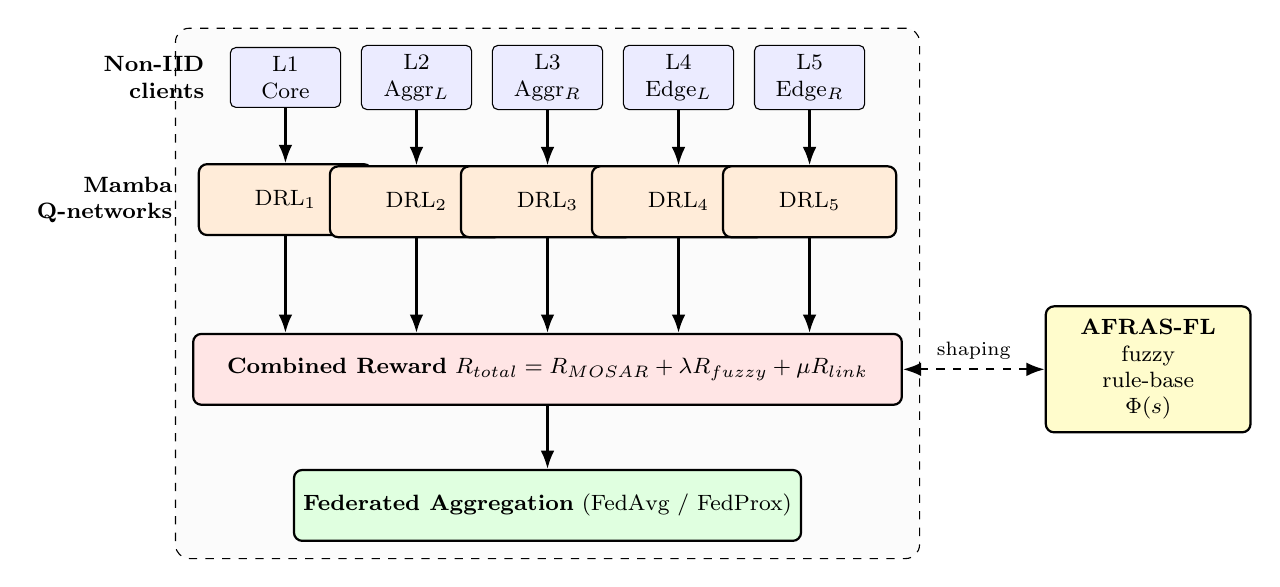
\begin{tikzpicture}[
      font=\footnotesize,
      client/.style={draw,rounded corners=2pt,fill=blue!8,minimum width=1.4cm,minimum height=0.7cm,align=center},
      module/.style={draw,rounded corners=3pt,fill=orange!15,minimum width=2.2cm,minimum height=0.9cm,align=center,thick},
      fed/.style={draw,rounded corners=3pt,fill=green!12,minimum width=3.2cm,minimum height=0.9cm,align=center,thick},
      reward/.style={draw,rounded corners=3pt,fill=red!10,minimum width=2.5cm,minimum height=0.9cm,align=center,thick},
      arr/.style={-Latex,thick},
      darr/.style={Latex-Latex,thick,dashed},
    ]
    % Client layer
    \node[client] (c1) {L1\\Core};
    \node[client,right=0.25cm of c1] (c2) {L2\\Aggr$_L$};
    \node[client,right=0.25cm of c2] (c3) {L3\\Aggr$_R$};
    \node[client,right=0.25cm of c3] (c4) {L4\\Edge$_L$};
    \node[client,right=0.25cm of c4] (c5) {L5\\Edge$_R$};
    \node[left=0.2cm of c1,align=right] (lbl) {\textbf{Non-IID}\\\textbf{clients}};

    % DRL agent layer
    \node[module,below=0.7cm of c1] (a1) {DRL$_1$};
    \node[module,below=0.7cm of c2] (a2) {DRL$_2$};
    \node[module,below=0.7cm of c3] (a3) {DRL$_3$};
    \node[module,below=0.7cm of c4] (a4) {DRL$_4$};
    \node[module,below=0.7cm of c5] (a5) {DRL$_5$};
    \node[left=0.2cm of a1,align=right] {\textbf{Mamba}\\\textbf{Q-networks}};

    \foreach \i in {1,...,5} {
      \draw[arr] (c\i) -- (a\i);
    }

    % Reward module (shared design)
    \node[reward,below=1.2cm of a3,minimum width=9cm] (rew)
      {\textbf{Combined Reward} $R_{\text{total}} = R_{\text{MOSAR}} + \lambda R_{\text{fuzzy}} + \mu R_{\text{link}}$};

    \foreach \i in {1,...,5} {
      \draw[arr] (a\i) -- (a\i |- rew.north);
    }

    % Federation layer
    \node[fed,below=0.8cm of rew] (fl) {\textbf{Federated Aggregation} (FedAvg / FedProx)};
    \draw[arr] (rew) -- (fl);

    % Fuzzy rule-base (side box)
    \node[module,right=1.8cm of rew,fill=yellow!20,minimum width=2.6cm,minimum height=1.6cm,align=center] (frb)
      {\textbf{AFRAS-FL}\\ fuzzy\\ rule-base\\ $\Phi(s)$};
    \draw[darr] (frb.west) -- node[above,sloped,font=\scriptsize]{shaping} (rew.east);

    % Dotted region label
    \begin{pgfonlayer}{background}
      \node[draw,dashed,rounded corners=5pt,fit=(c1)(c5)(a1)(a5)(rew)(fl),inner sep=6pt,fill=gray!3] (sys) {};
    \end{pgfonlayer}
  \end{tikzpicture}%
  }
  \caption{High-level overview of the proposed system. Five non-IID SDN
  clients run local Mamba-based DRL agents whose reward signal is the
  combined MOSAR+fuzzy+link reward
  ($R_{\text{total}}$). The AFRAS-FL rule-base (yellow, right) mines
  IF--THEN fuzzy rules from the agents' experience and emits a
  potential-based shaping signal $\gamma\Phi(s')-\Phi(s)$ that is added
  to the reward before the federated aggregation step.}
  \label{fig:system_overview}
\end{figure}
% ---------- /SYSTEM OVERVIEW ----------

% ============================================================================
\section{Results}\label{sec:results}
% ============================================================================

Six questions structure the empirical study: (R1) Does
fuzzy-augmented shaping accelerate convergence relative to the
federated baselines? (R2) What does the extracted fuzzy rule-base
look like, and is it interpretable? (R3) How does the framework
behave across the four federated training phases? (R4) Is the
backbone selection robust under different sensitivity scenarios?
(R5) Does the explainable feature selection survive federated
aggregation? (R6) How does the full pipeline compare against a
purpose-built federated multi-agent DQN baseline, and what is its
operational envelope across the two benchmarks? We take these
questions in turn.

% ----------------------------------------------------------------------------
\subsection{Fuzzy-augmented shaping accelerates and stabilises
convergence}\label{sec:r1_convergence}

Starting with R1, we trained the same Mamba-based DRL
backbone\cite{gu2023mamba,gu2022efficiently} under three reward
variants: a sparse reward, a dense MOSAR-only reward, and the full
$R_{\text{total}} = R_{\text{MOSAR}} + \lambda R_{\text{fuzzy}} +
\mu R_{\text{link}}$. Figures~\ref{fig:fl_convergence}
and~\ref{fig:agent_heatmap} plot the resulting federated
convergence curves on CICIoT2023.

\begin{figure}[!htbp]
  \centering
  \begin{subfigure}{0.32\linewidth}
    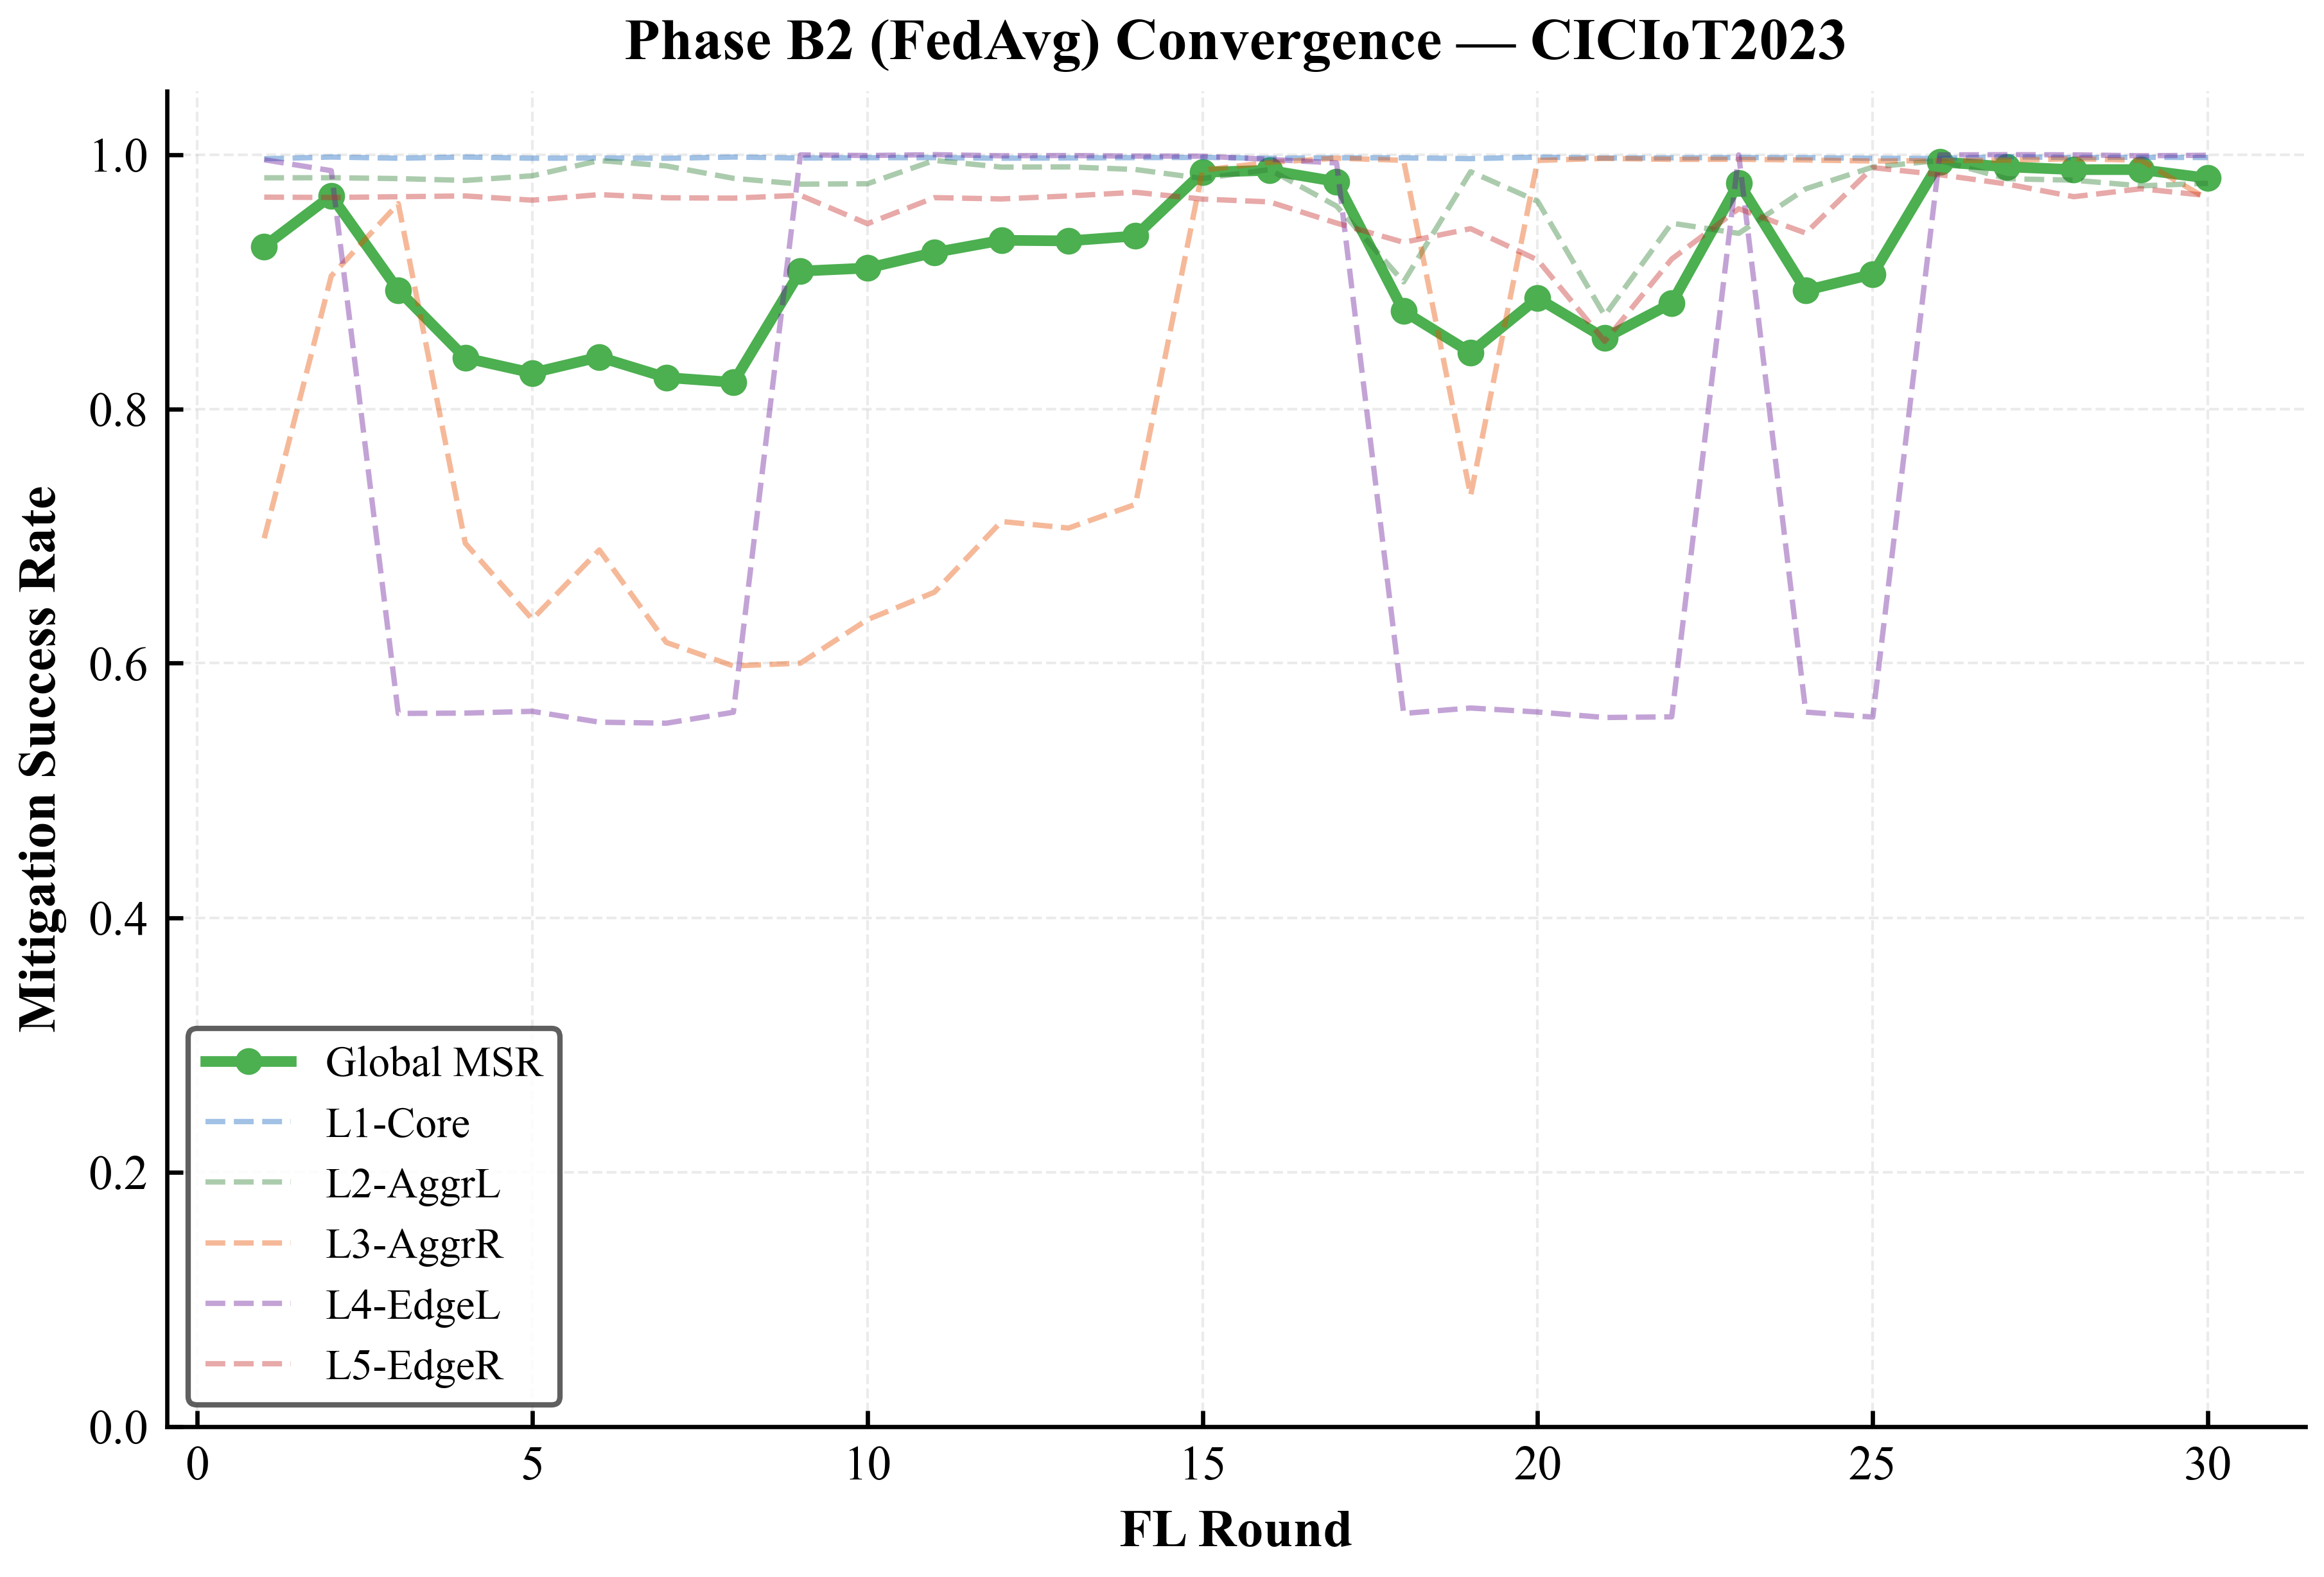
\includegraphics[width=\linewidth]{strategyB_ciciot2023/04_FL/fig13_fedavg_convergence.png}
    \caption{FedAvg}
  \end{subfigure}
  \hfill
  \begin{subfigure}{0.32\linewidth}
    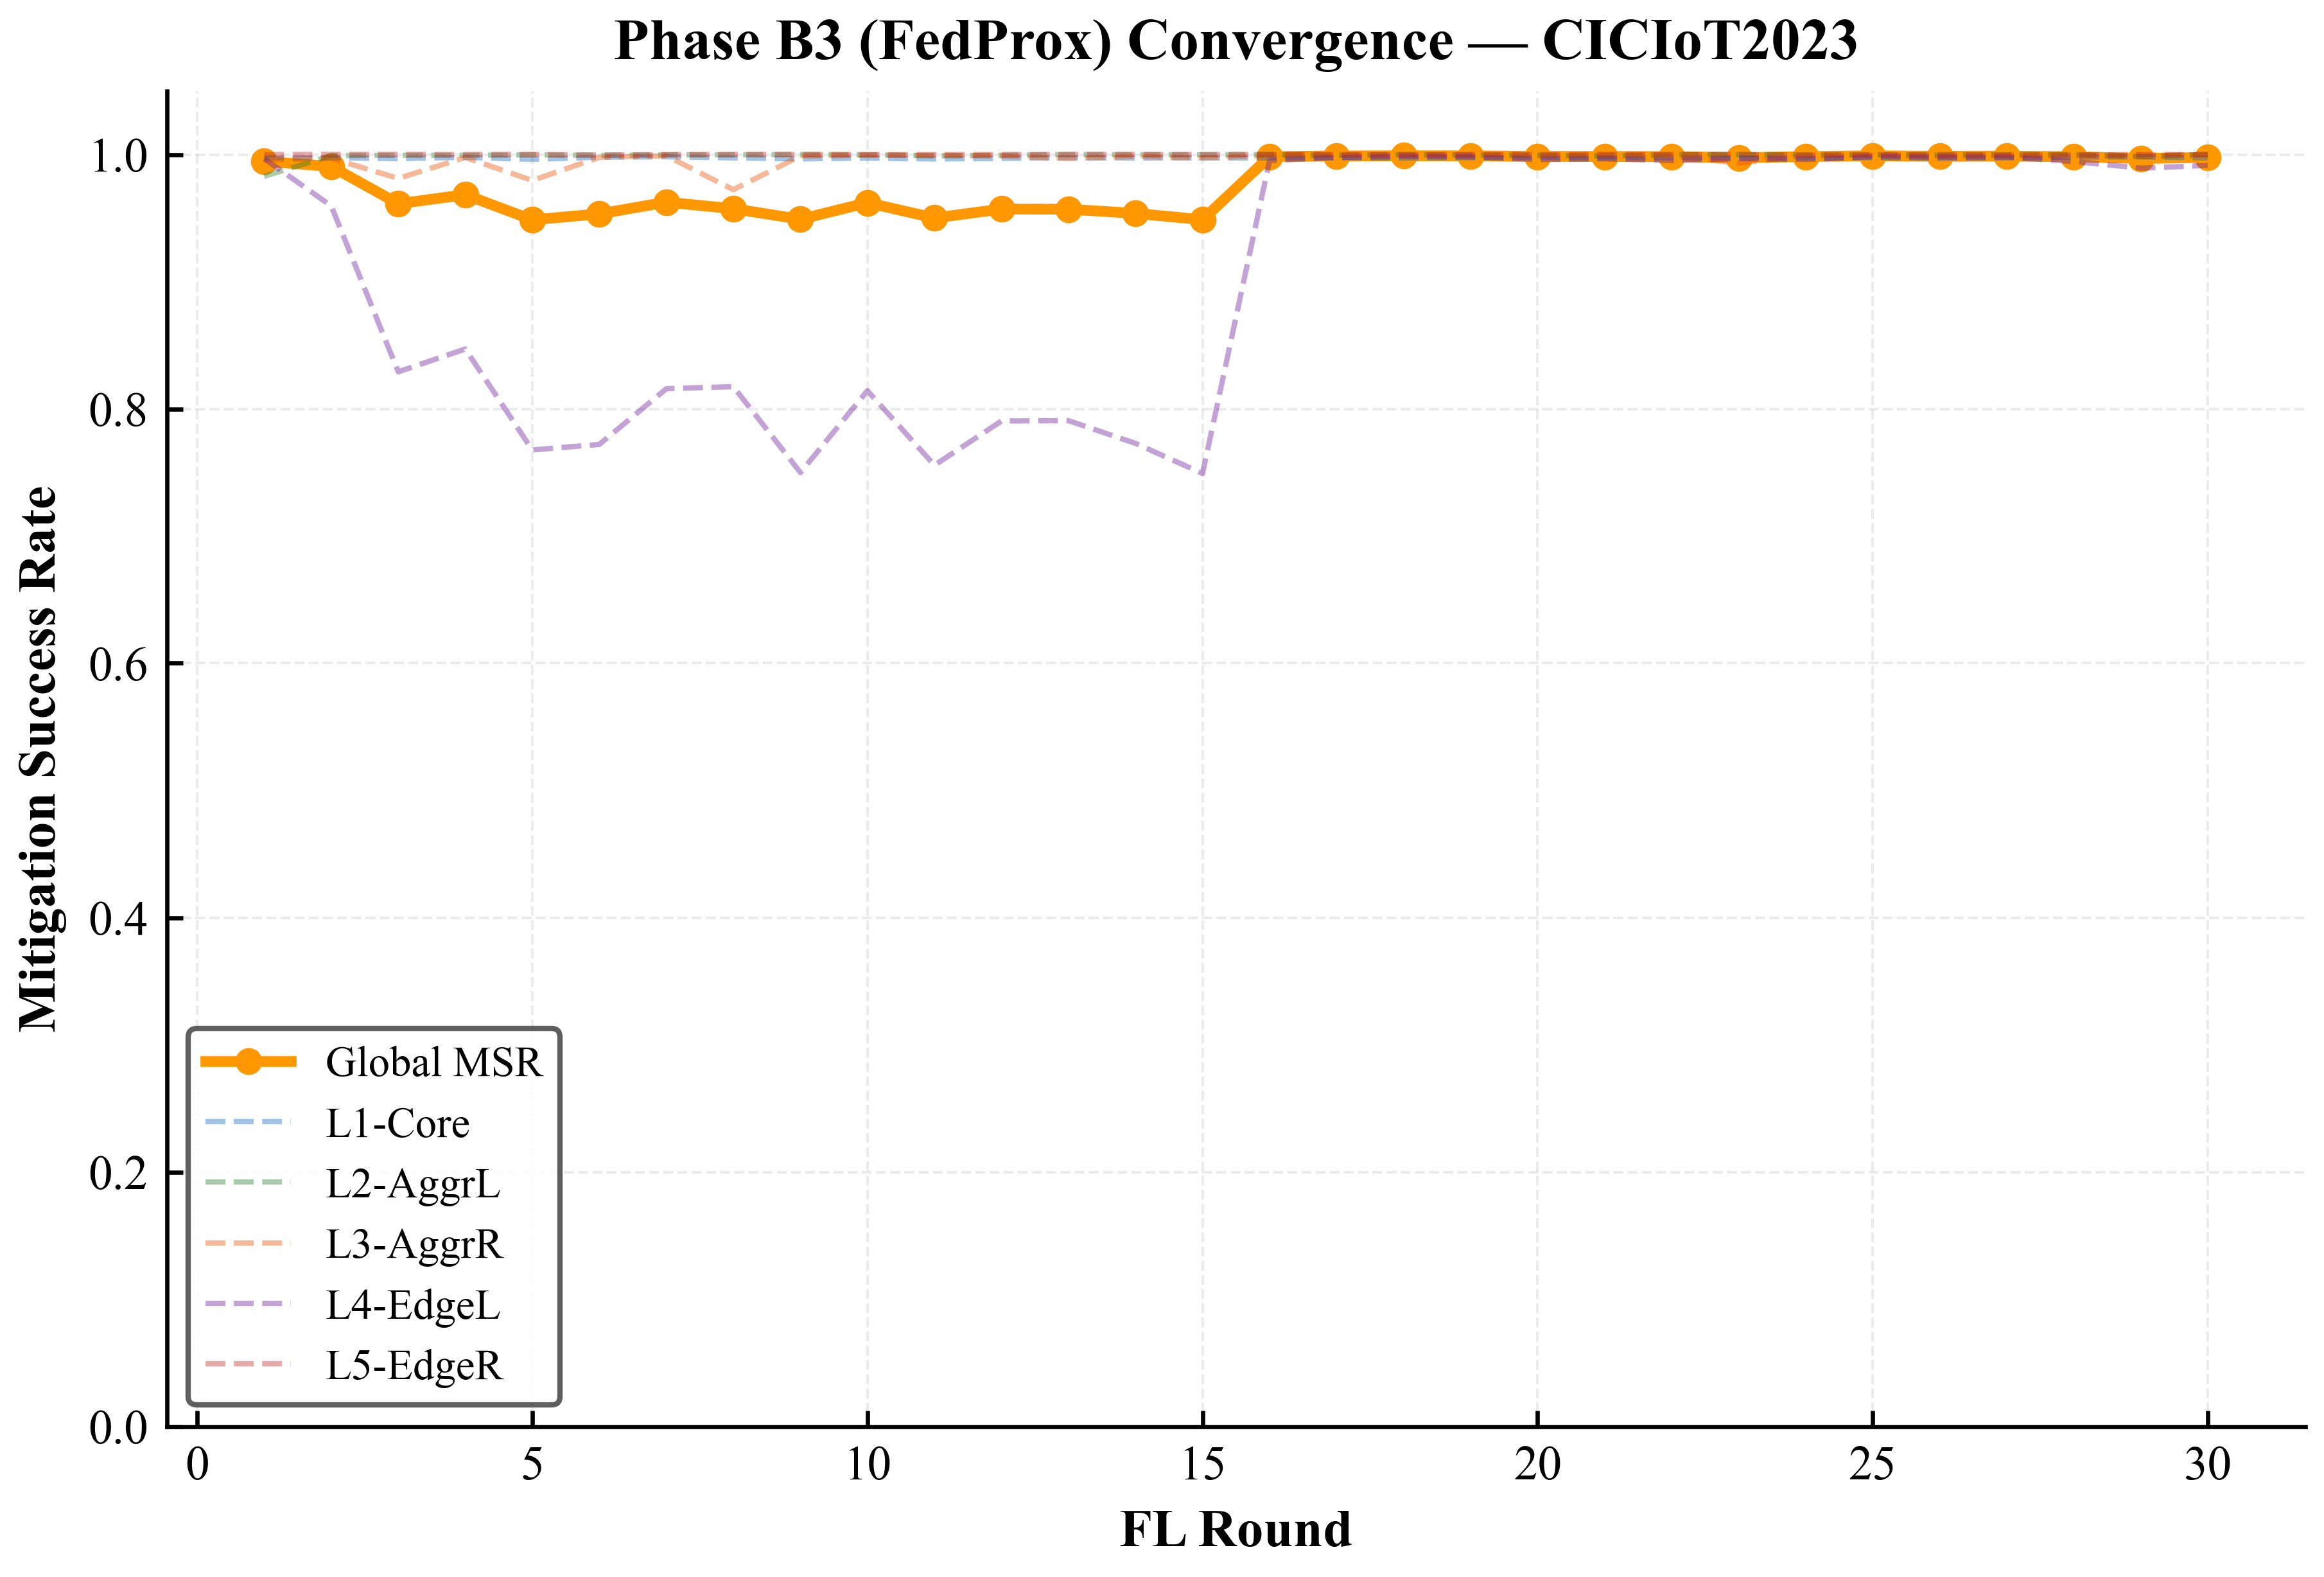
\includegraphics[width=\linewidth]{strategyB_ciciot2023/04_FL/fig14_fedprox_convergence.png}
    \caption{FedProx}
  \end{subfigure}
  \hfill
  \begin{subfigure}{0.32\linewidth}
    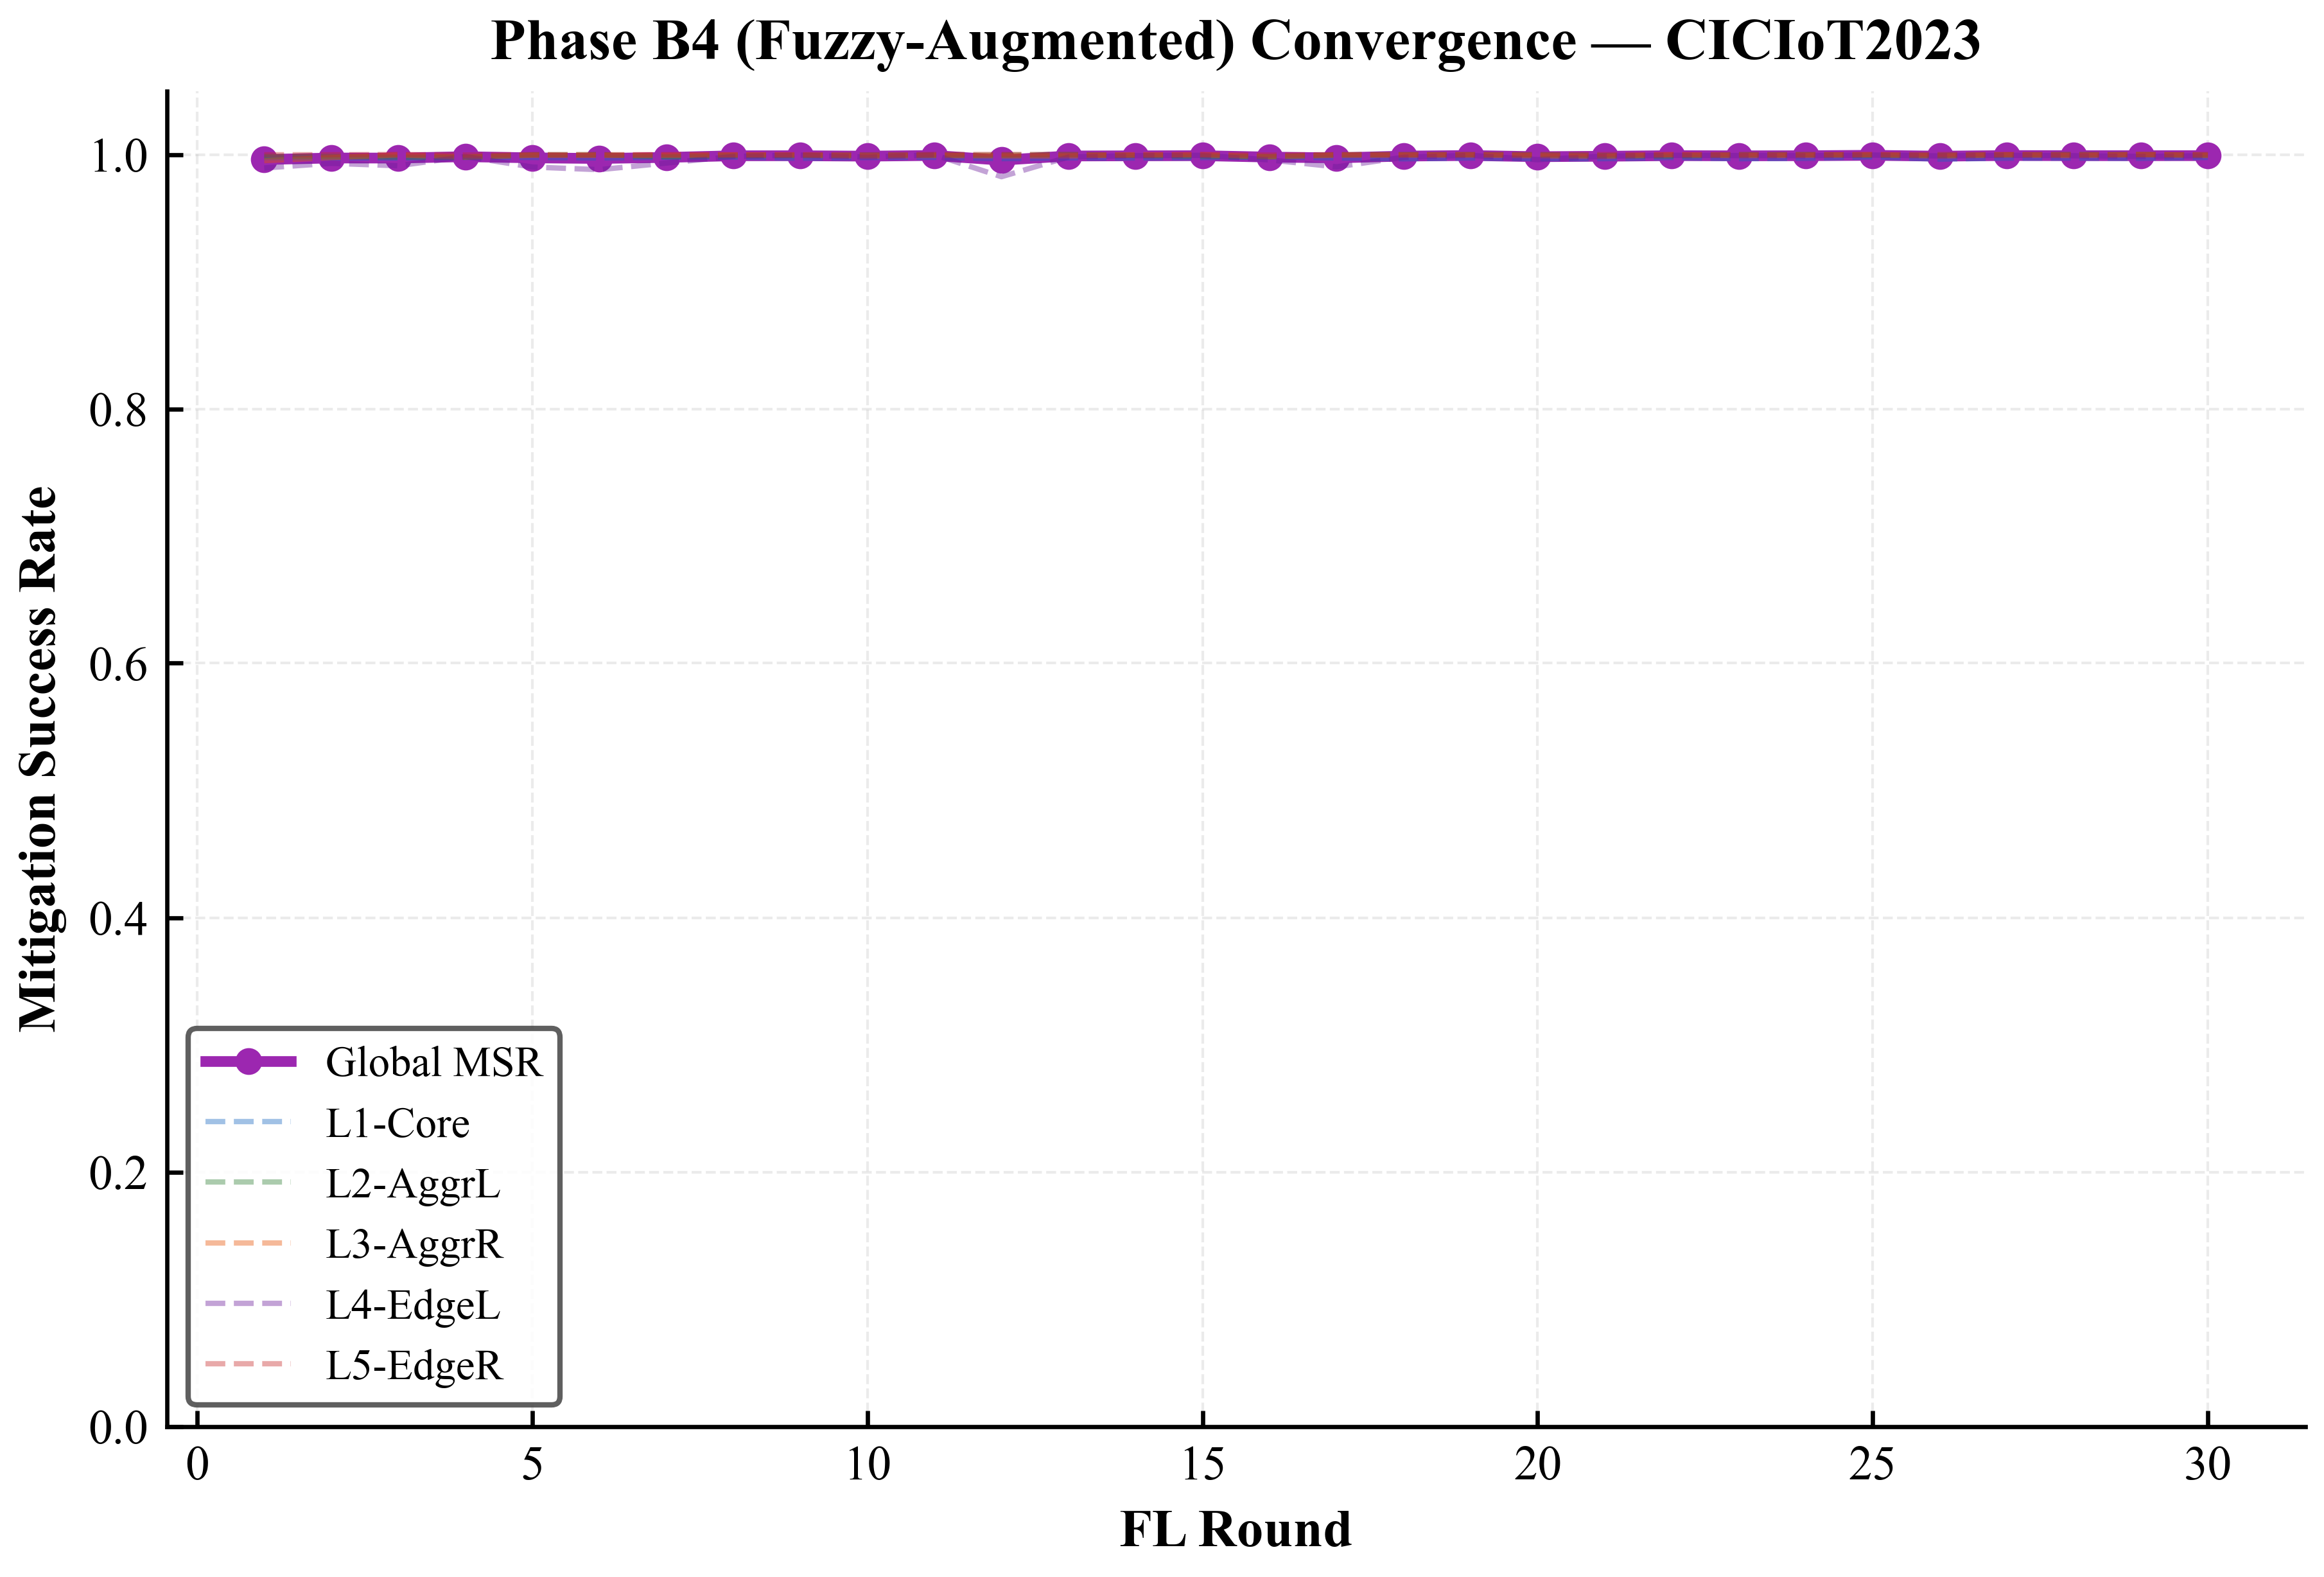
\includegraphics[width=\linewidth]{strategyB_ciciot2023/04_FL/fig15_fuzzy_convergence.png}
    \caption{Fuzzy-augmented (ours)}
  \end{subfigure}
  \caption{Federated convergence on CICIoT2023 across five non-IID clients.
  Fuzzy-augmented shaping reaches a higher and more stable plateau than
  FedAvg and FedProx alone.}\label{fig:fl_convergence}
\end{figure}

\begin{figure}[!htbp]
  \centering
  \begin{subfigure}{0.48\linewidth}
    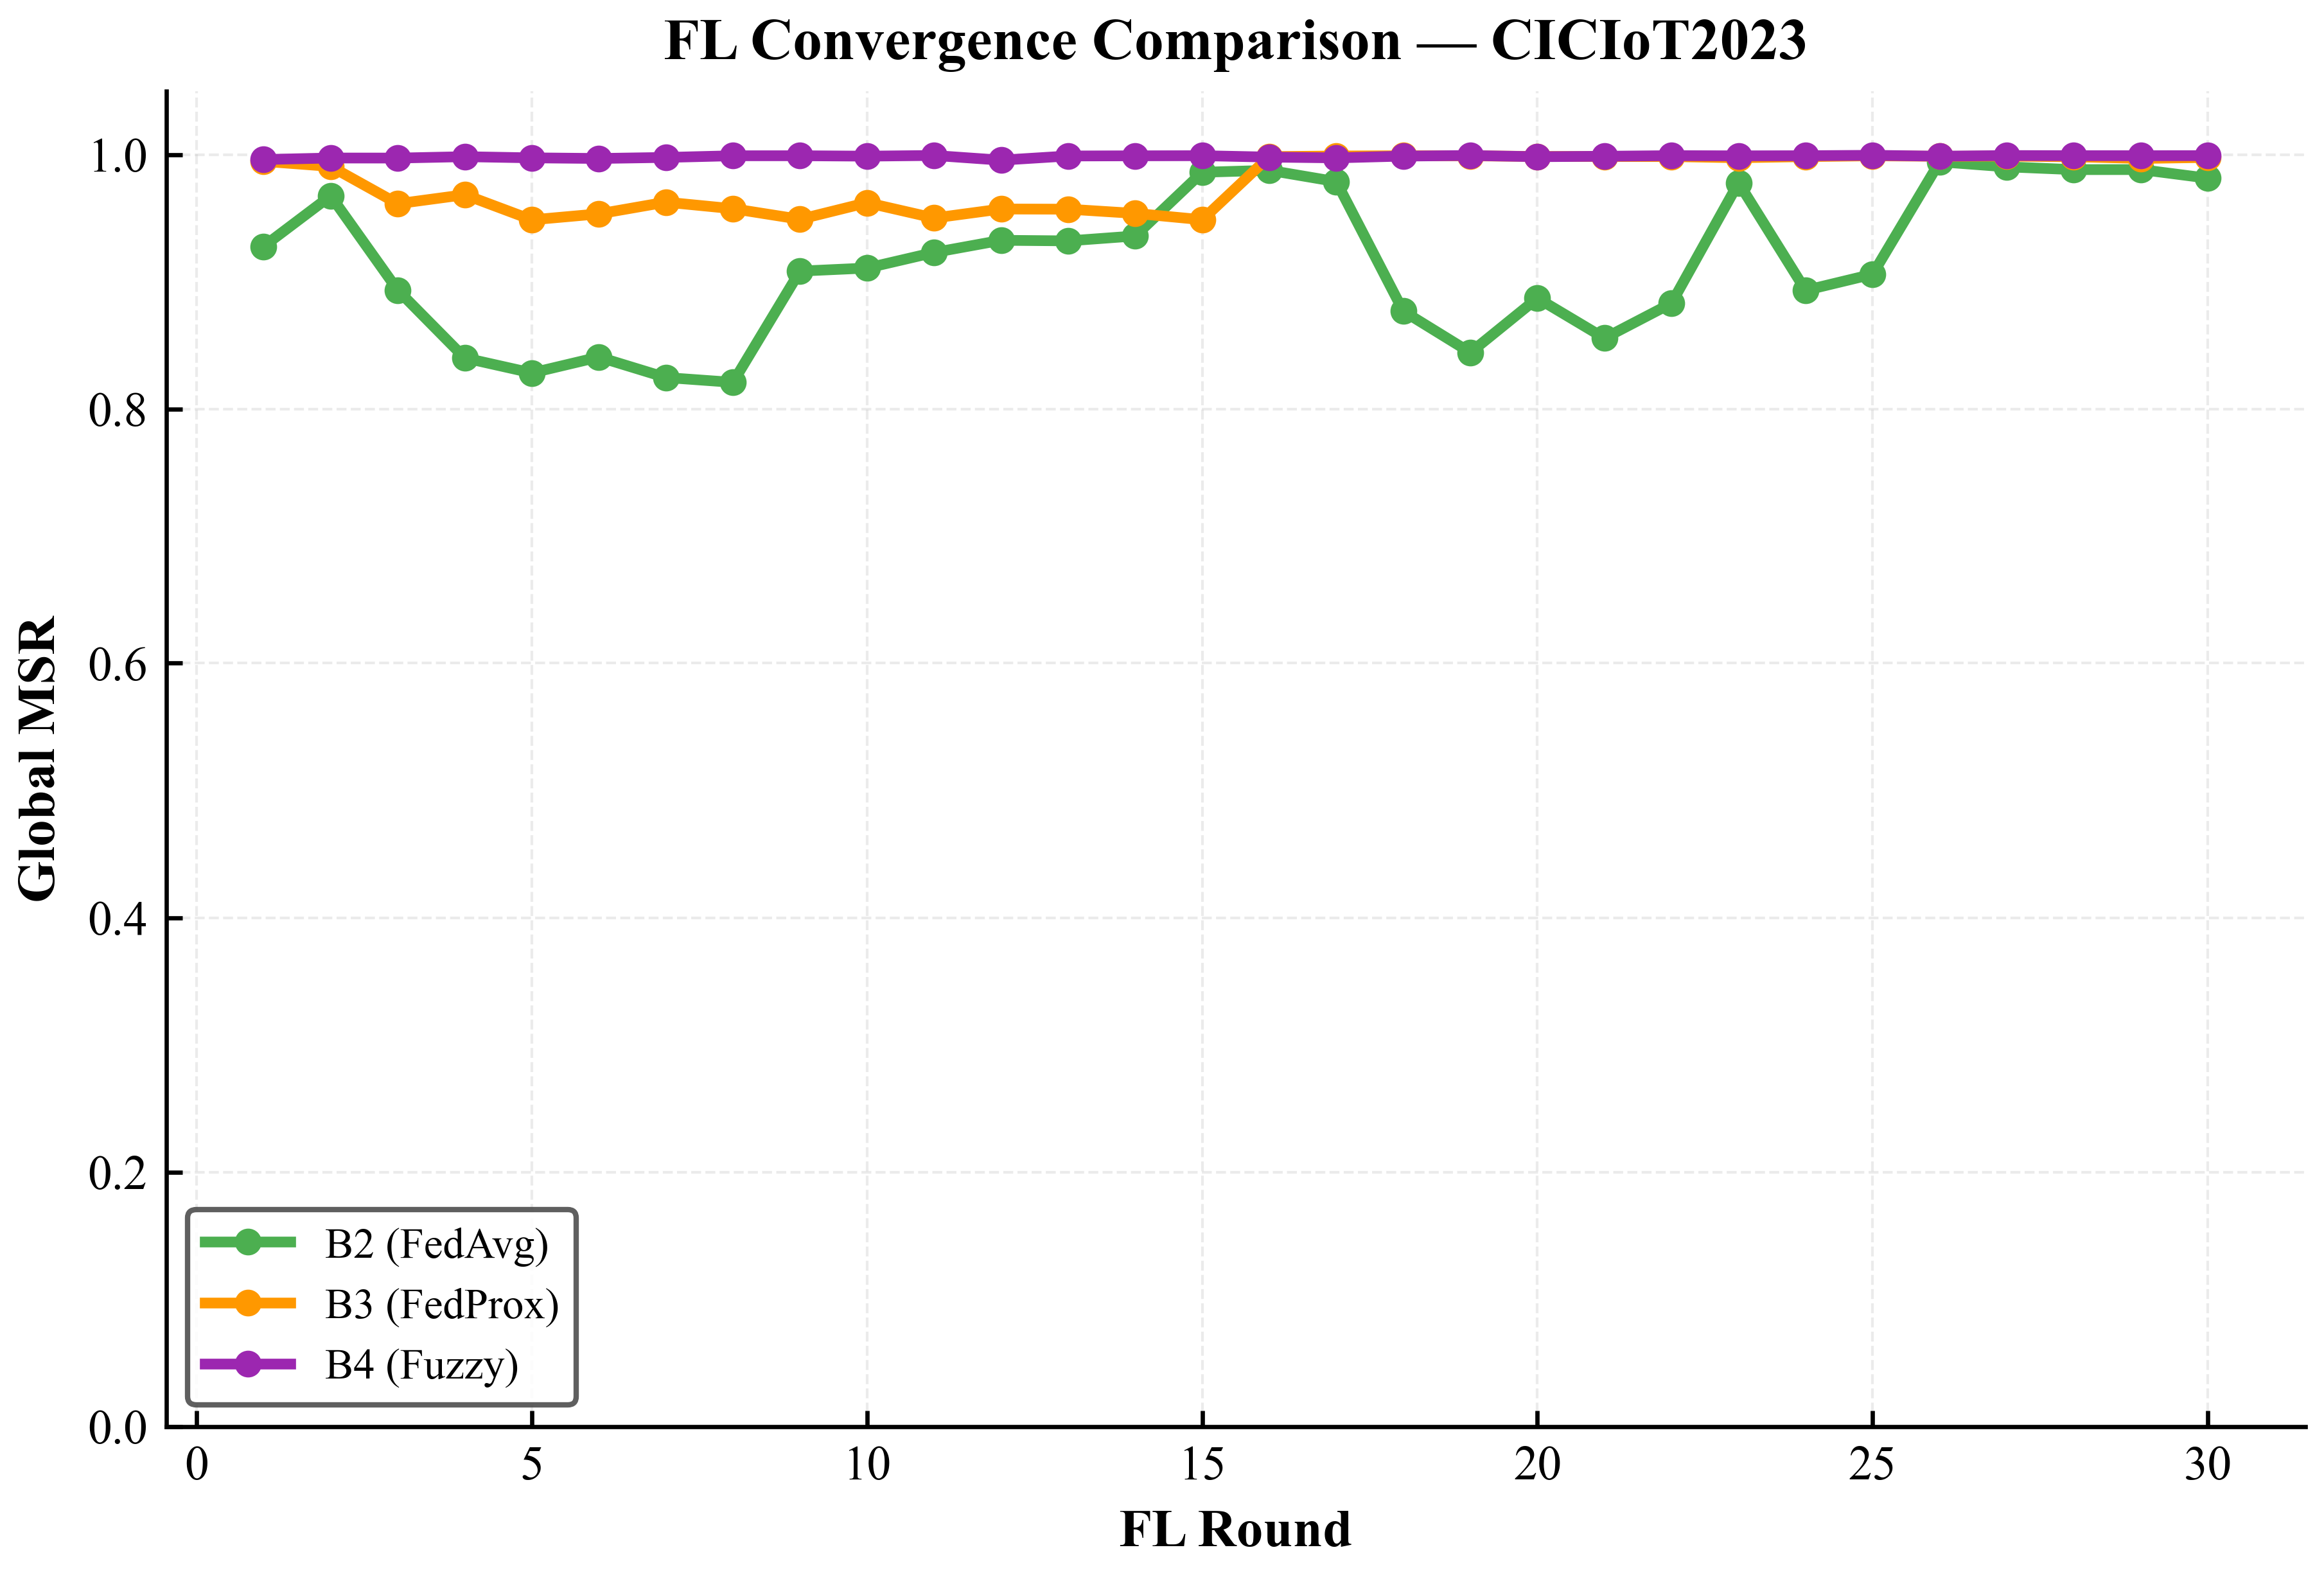
\includegraphics[width=\linewidth]{strategyB_ciciot2023/04_FL/fig20_convergence_overlay.png}
    \caption{Convergence overlay (CICIoT2023)}
  \end{subfigure}
  \hfill
  \begin{subfigure}{0.48\linewidth}
    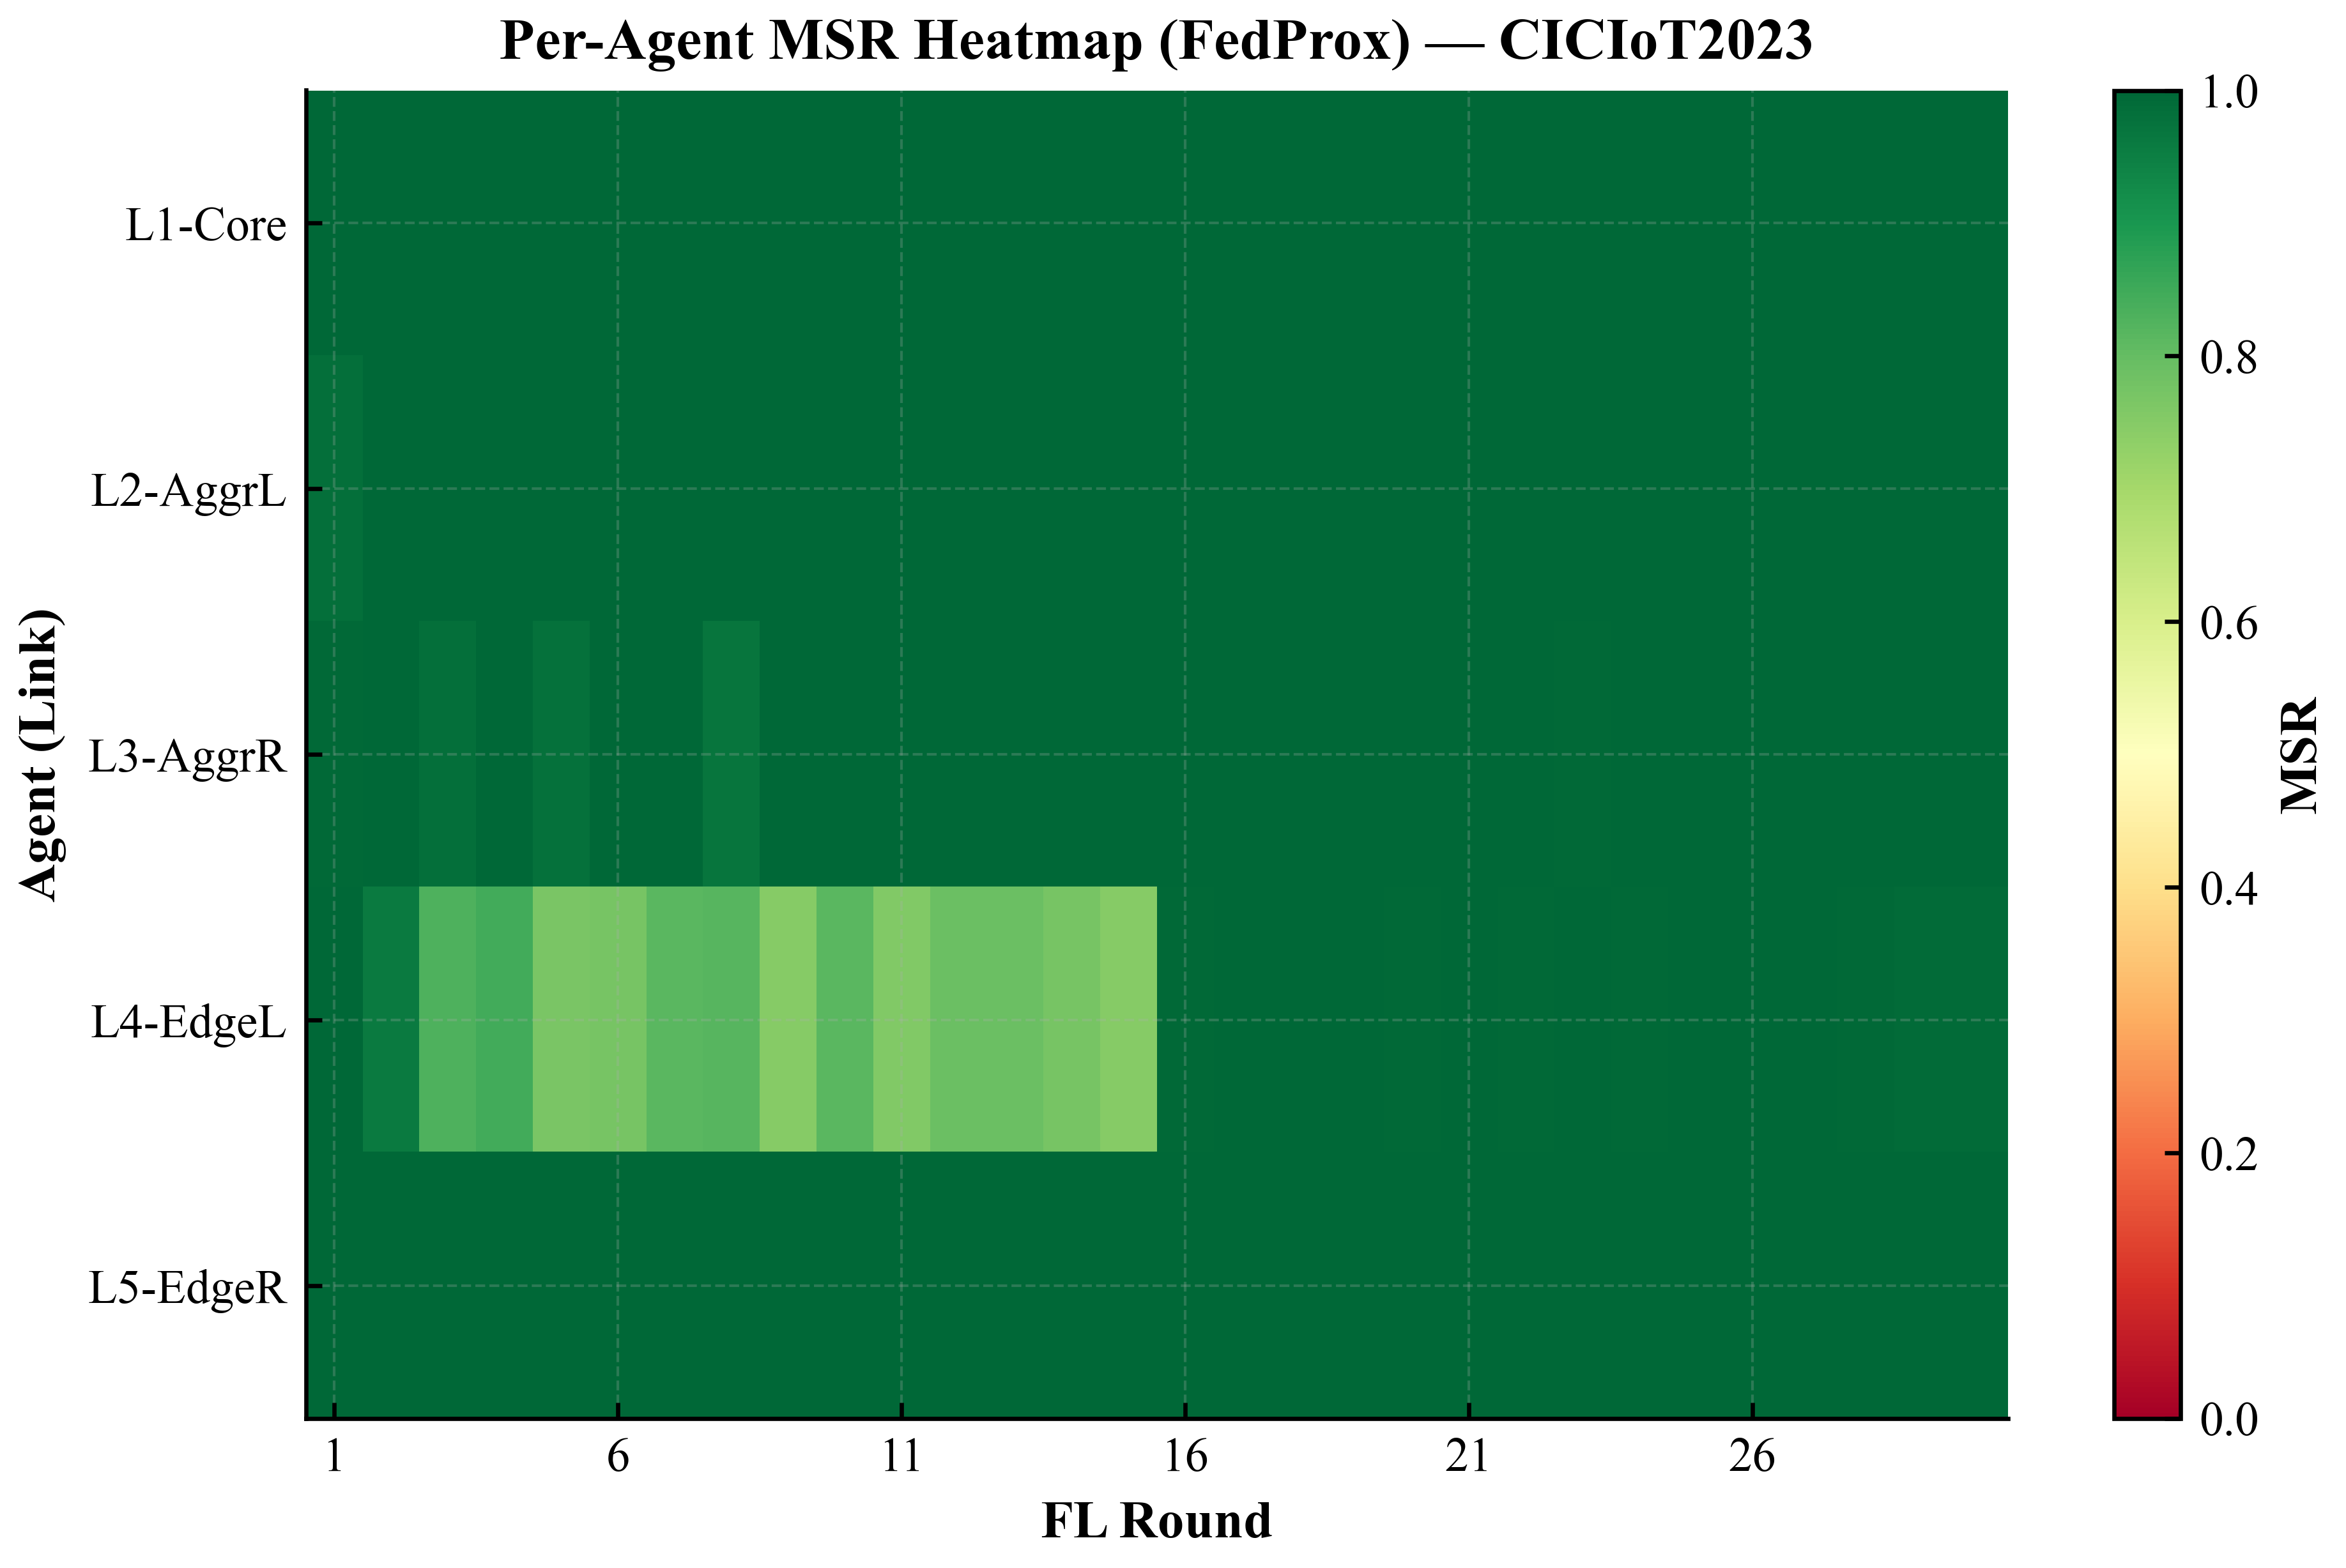
\includegraphics[width=\linewidth]{strategyB_ciciot2023/04_FL/fig21_agent_heatmap.png}
    \caption{Per-agent reward heatmap}
  \end{subfigure}
  \caption{Per-agent dynamics under fuzzy-augmented shaping. The five
  non-IID clients converge into a tight band, indicating that the shaping
  signal mitigates client drift.}\label{fig:agent_heatmap}
\end{figure}

Zooming into the reward signal itself, the MOSAR breakdown
(Fig.~\ref{fig:mosar_breakdown}) shows that all five components
contribute non-trivially: detection and accuracy dominate, latency
and confidence smooth the curve, and the impact term keeps the
false-positive penalty active throughout training. The composition
of these five signals is what the fuzzy rule-base will later mine,
which brings us to R2.

\begin{figure}[!htbp]
  \centering
  \begin{subfigure}{0.48\linewidth}
    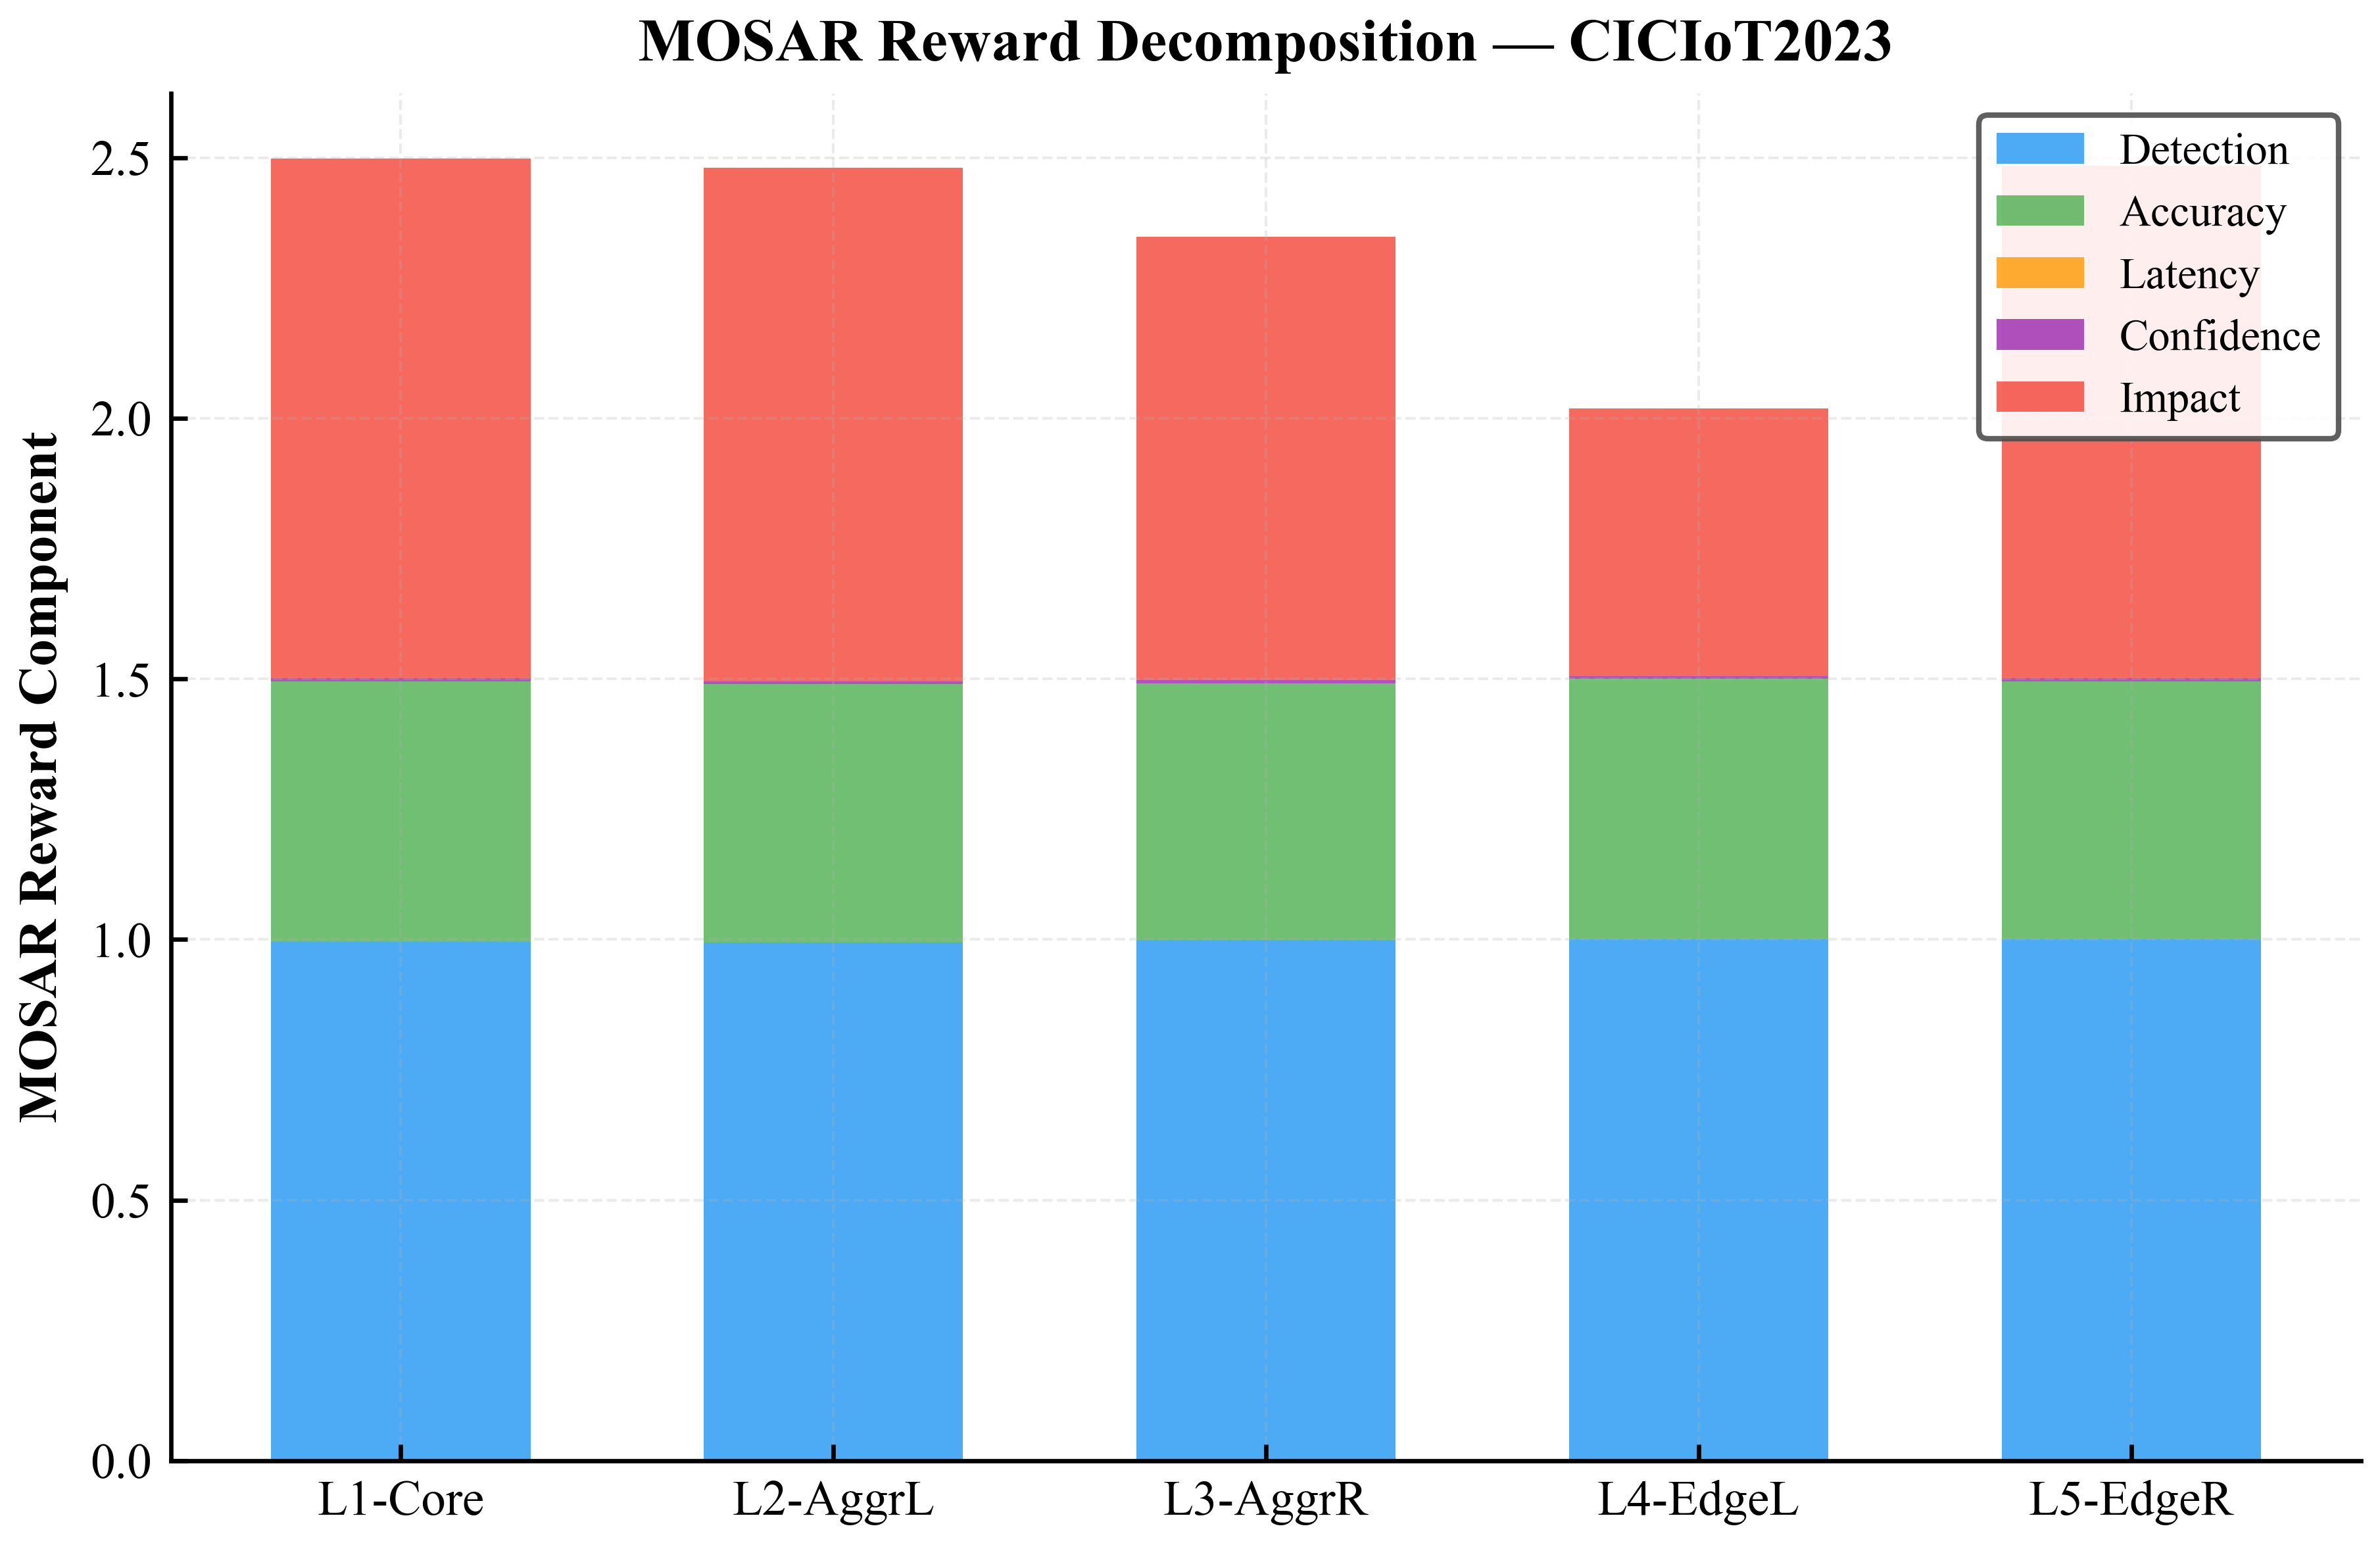
\includegraphics[width=\linewidth]{strategyB_ciciot2023/03_MOSAR_DQN/fig11_mosar_breakdown.png}
    \caption{MOSAR component breakdown}
  \end{subfigure}
  \hfill
  \begin{subfigure}{0.48\linewidth}
    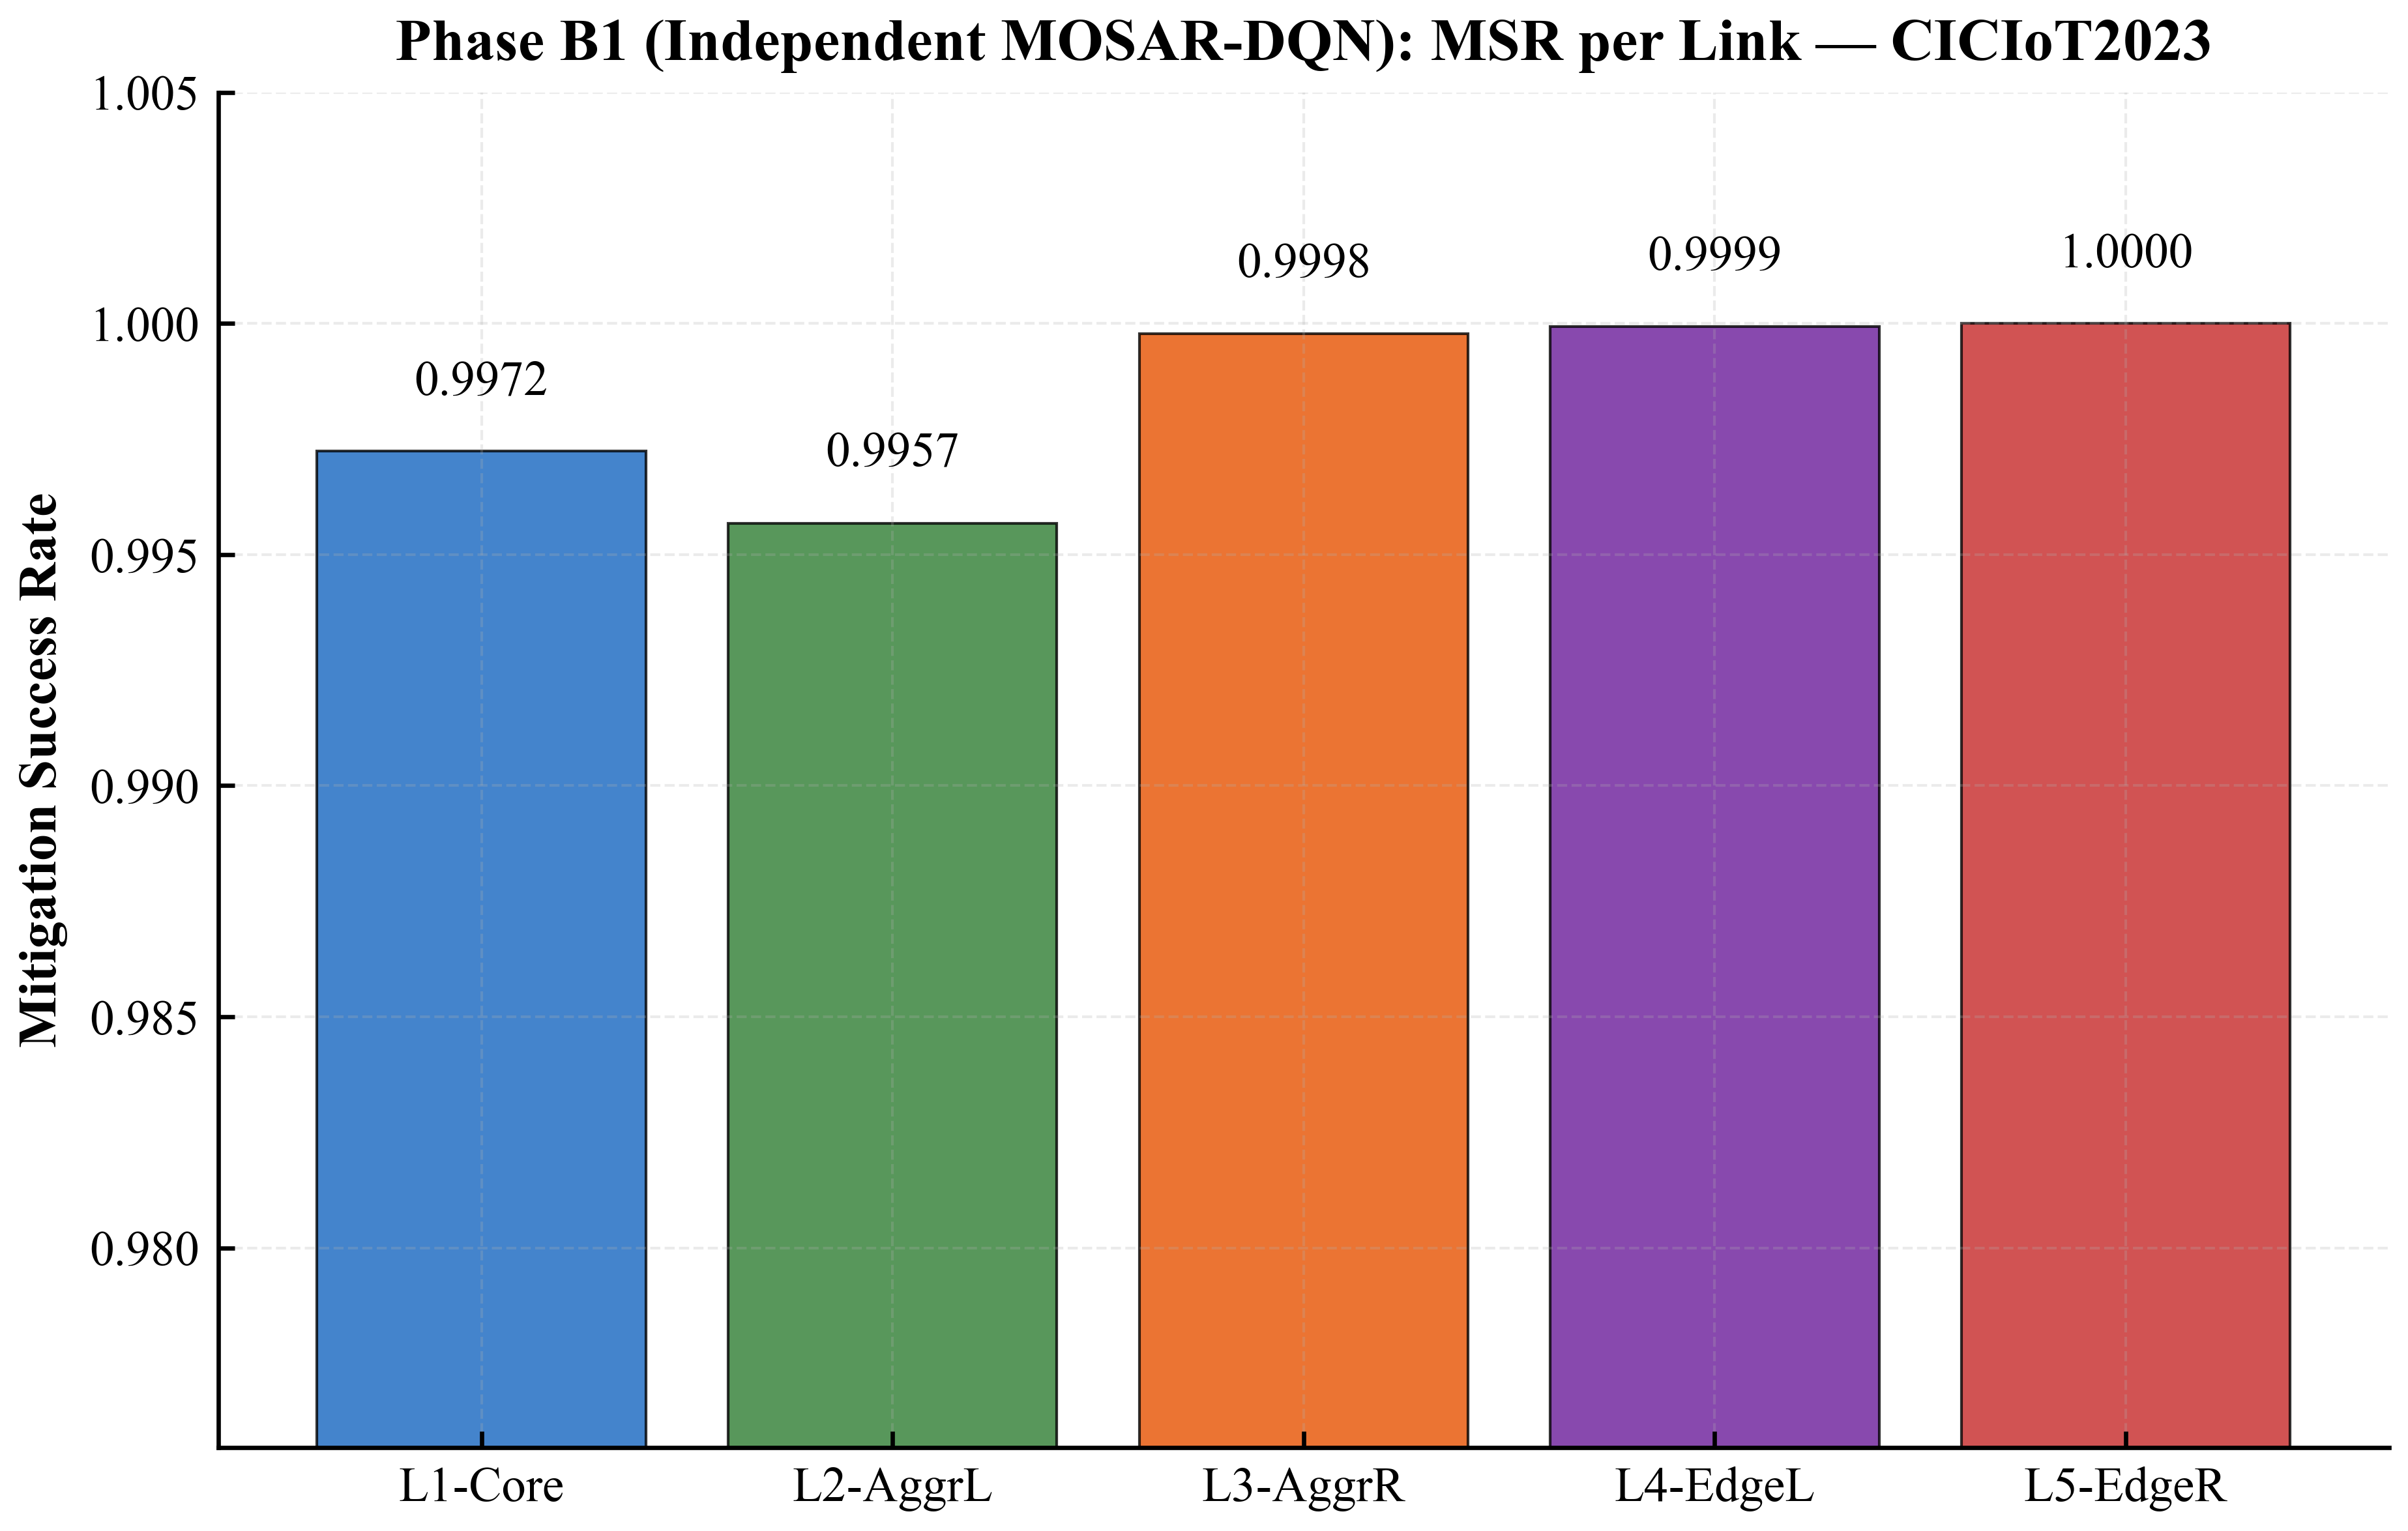
\includegraphics[width=\linewidth]{strategyB_ciciot2023/03_MOSAR_DQN/fig12_b1_msr.png}
    \caption{Phase-B1 MSR trajectory}
  \end{subfigure}
  \caption{MOSAR reward decomposition and the resulting Mean Success Rate
  (MSR) trajectory of the federated DRL agent during the first training
  phase.}\label{fig:mosar_breakdown}
\end{figure}

% ----------------------------------------------------------------------------
\subsection{Fuzzy rule-base is compact and
interpretable}\label{sec:r2_rules}

AFRAS-FL extracts between $4$ and $9$ rules per client on CICIoT2023
and $6$--$7$ rules per client on DIAD2024, with average rule
confidence in the range $[0.76, 1.00]$ on CICIoT2023 and
$[0.999, 1.000]$ on DIAD2024 (Table~\ref{tab:phase_b0}). The rules
are mined directly from agent transitions: a state pattern that is
consistently followed by an action yielding high MOSAR reward
becomes a candidate, which is then pruned by support and confidence
thresholds.

These counts describe the \emph{output} of the rule miner; to see
the machinery behind them, Fig.~\ref{fig:rule_mining} visualises the
rule-mining stage on the core link of CICIoT2023, covering signal
vs.\ noise separation, density estimation, adaptive grid
classification, and the resulting boundary map.

\begin{figure}[!htbp]
  \centering
  \begin{subfigure}{0.32\linewidth}
    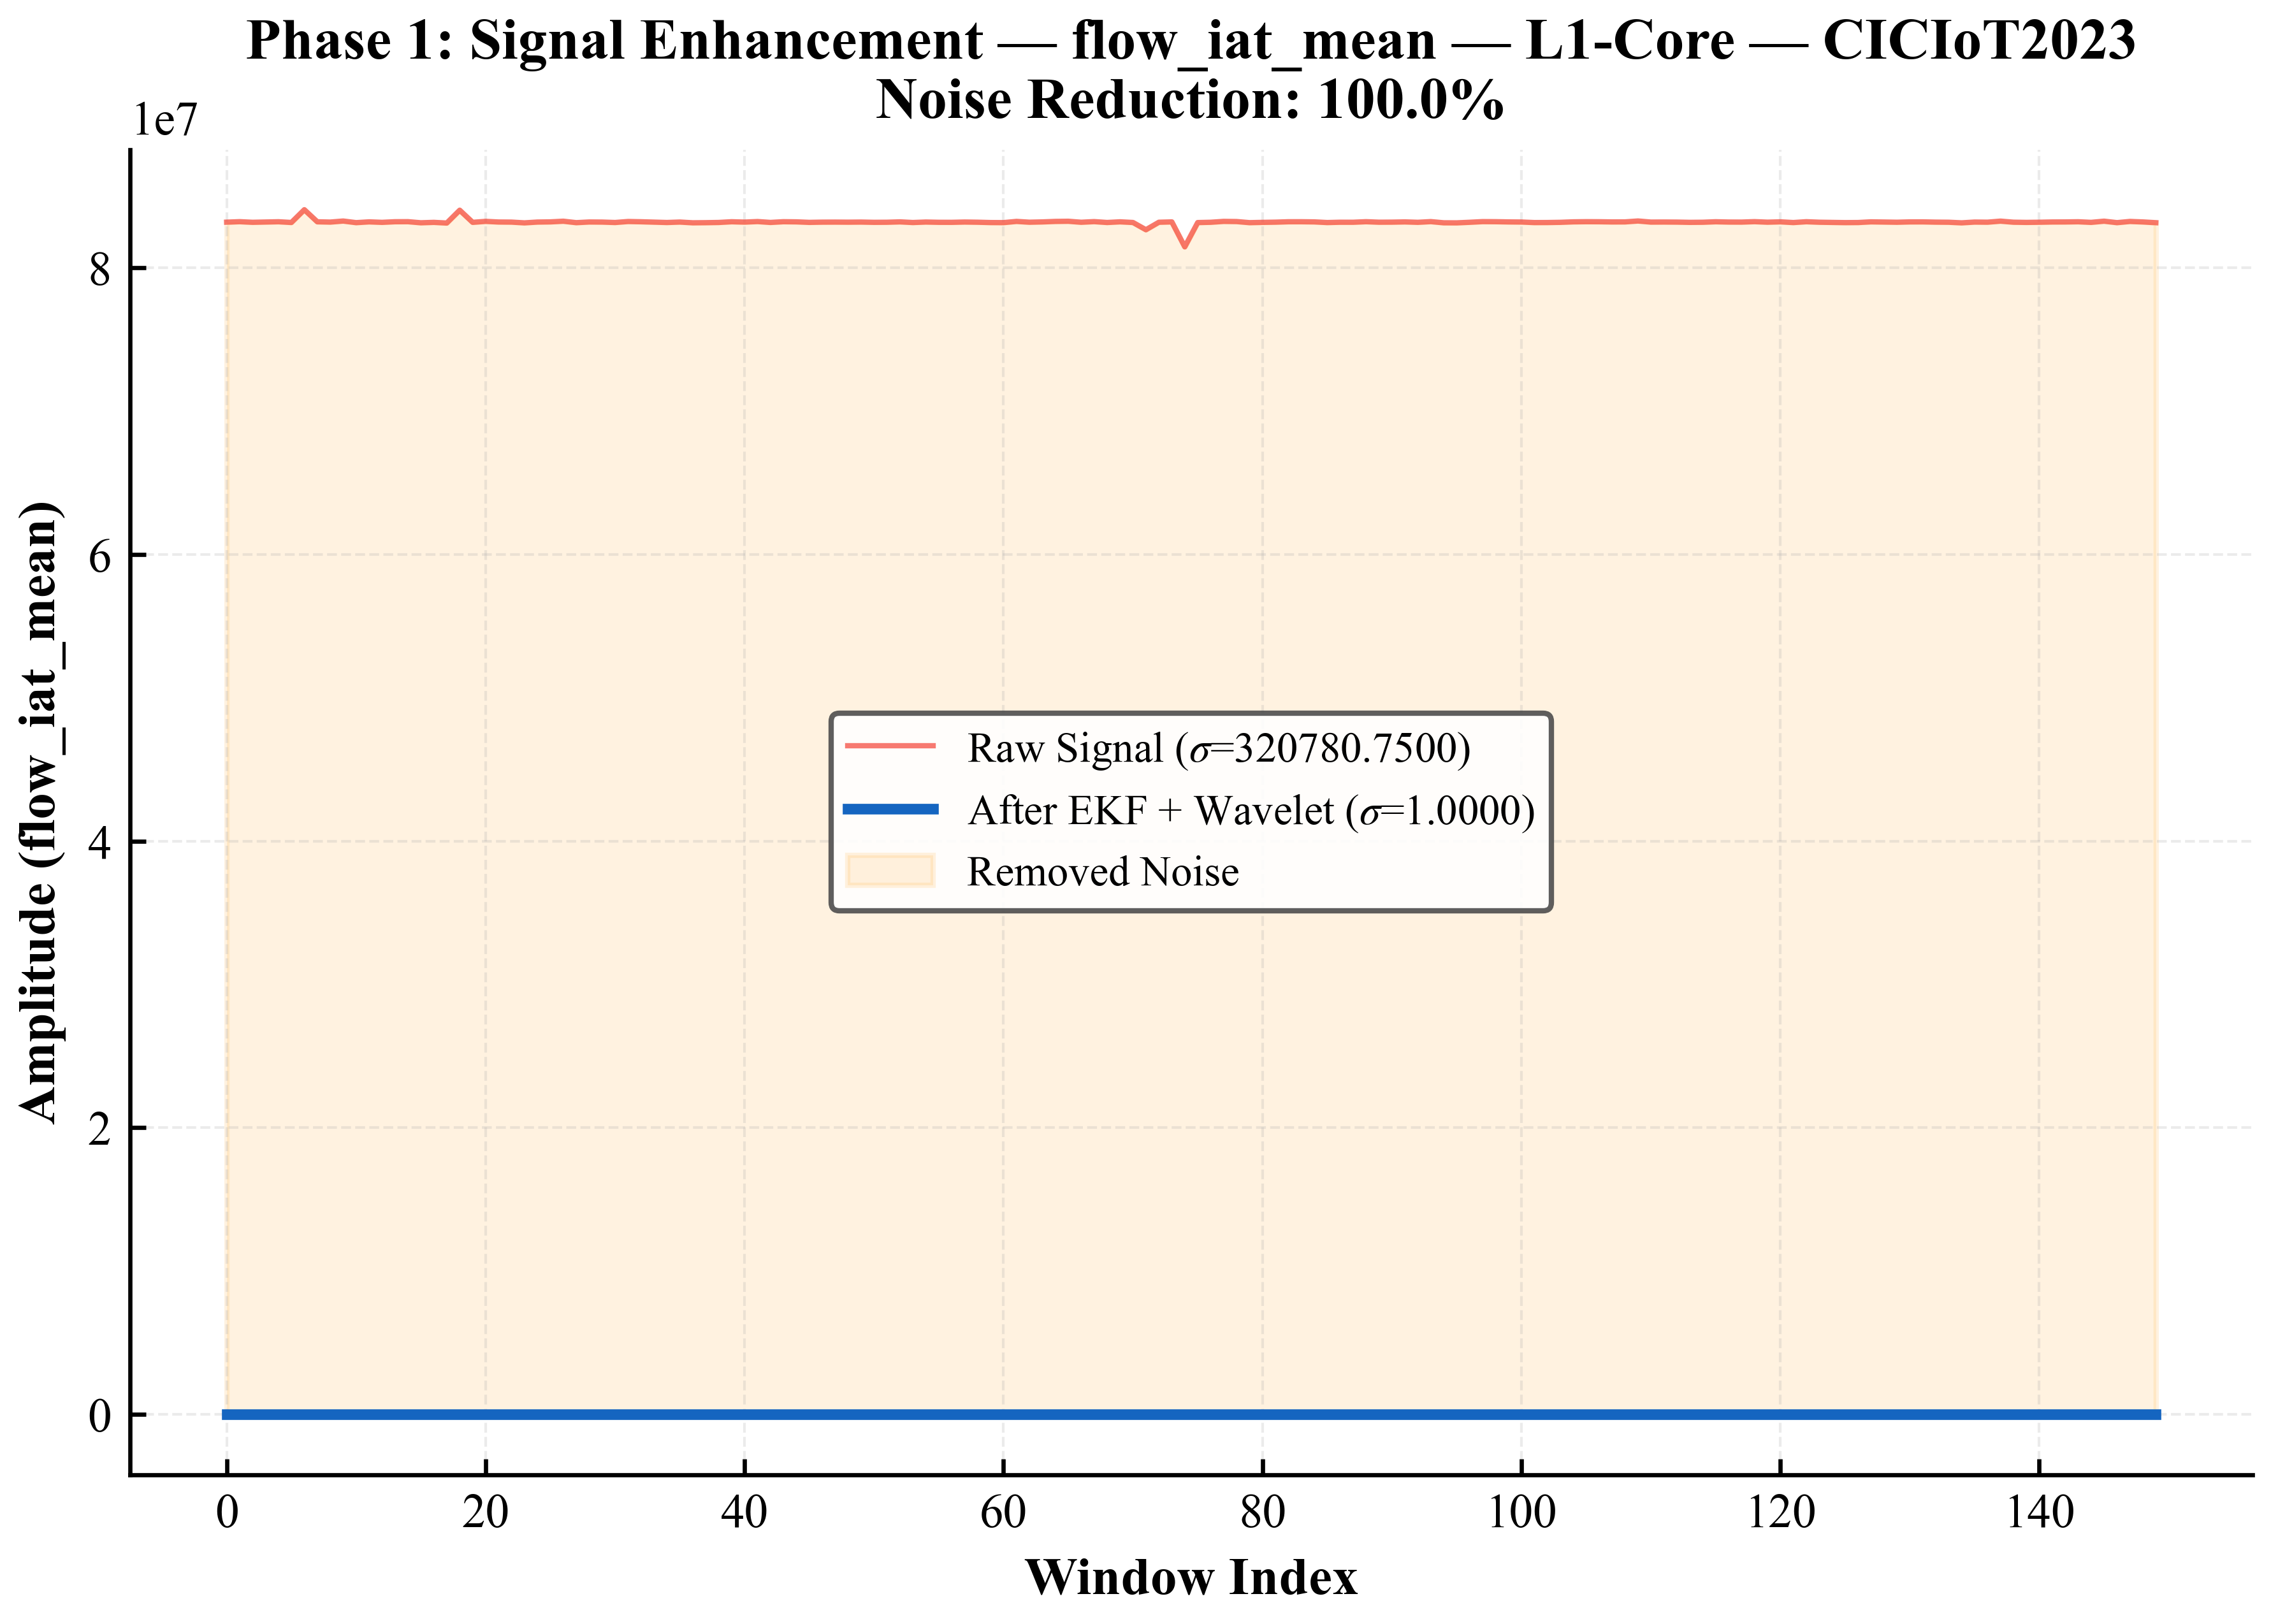
\includegraphics[width=\linewidth]{strategyB_ciciot2023/01_AFRAS_FL/fig01a_signal_flow_iat_mean_L1_Core.png}
    \caption{Signal flow}
  \end{subfigure}
  \hfill
  \begin{subfigure}{0.32\linewidth}
    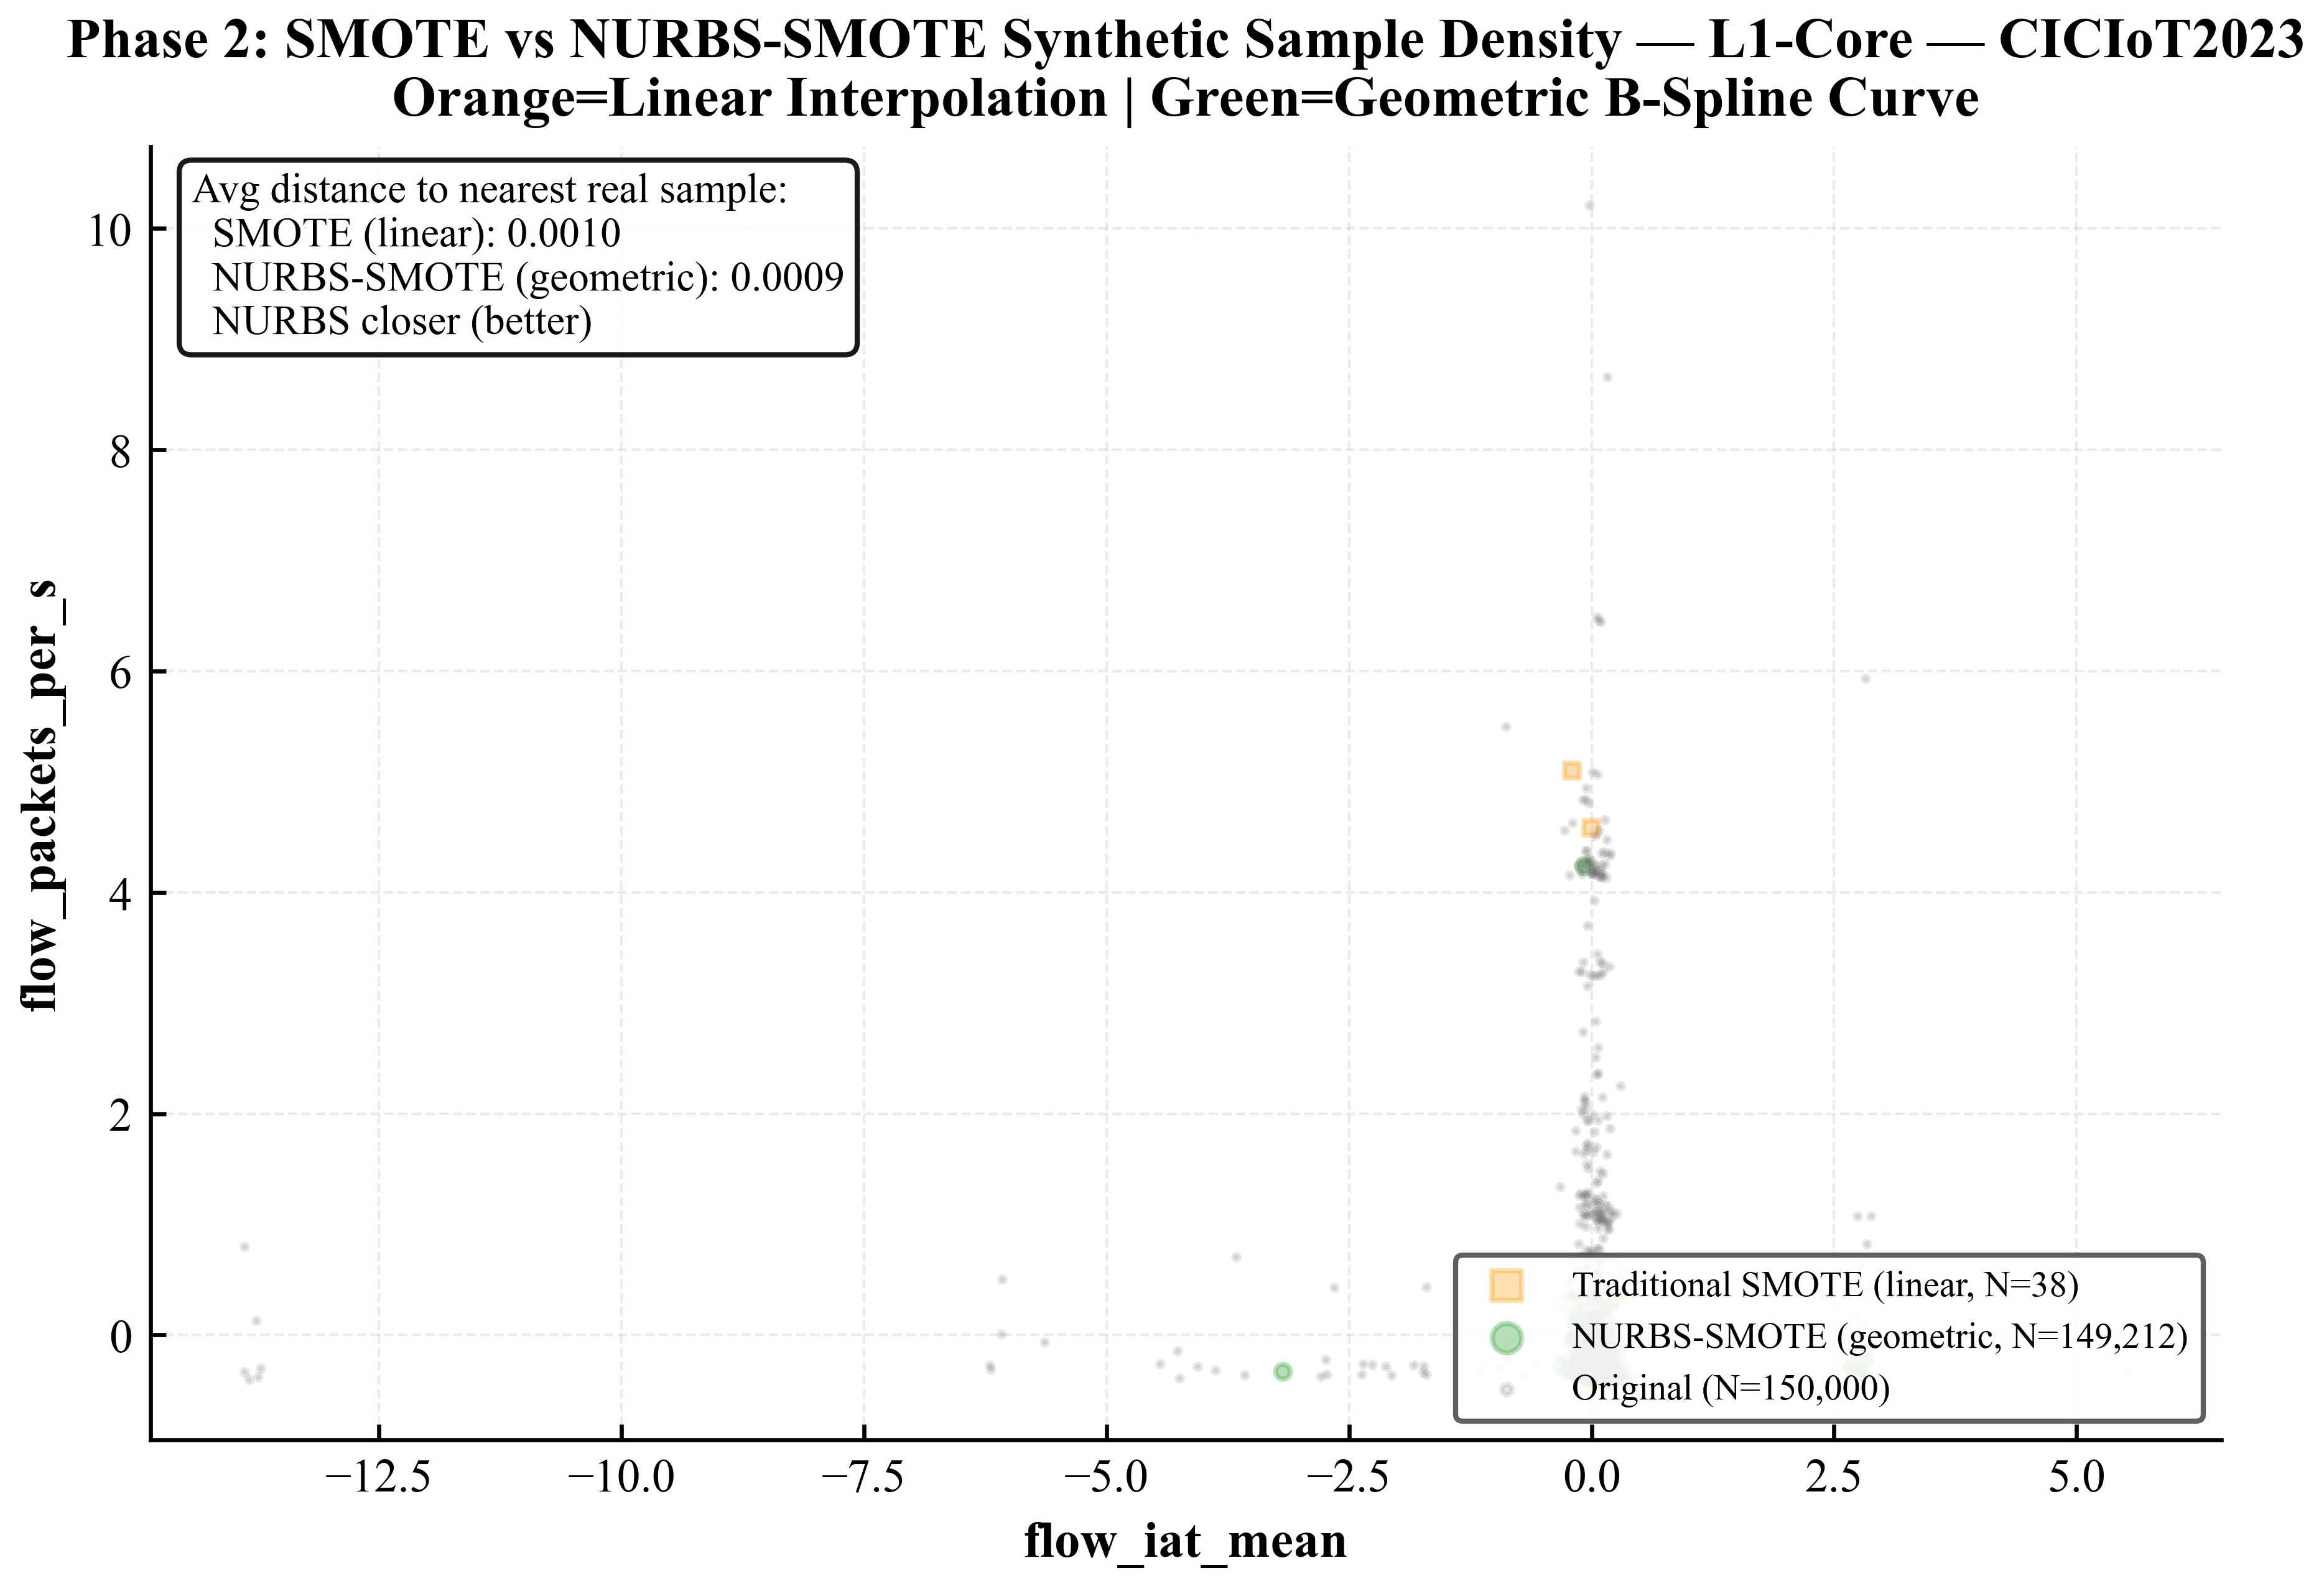
\includegraphics[width=\linewidth]{strategyB_ciciot2023/01_AFRAS_FL/fig02b_density_L1_Core.png}
    \caption{Density estimate}
  \end{subfigure}
  \hfill
  \begin{subfigure}{0.32\linewidth}
    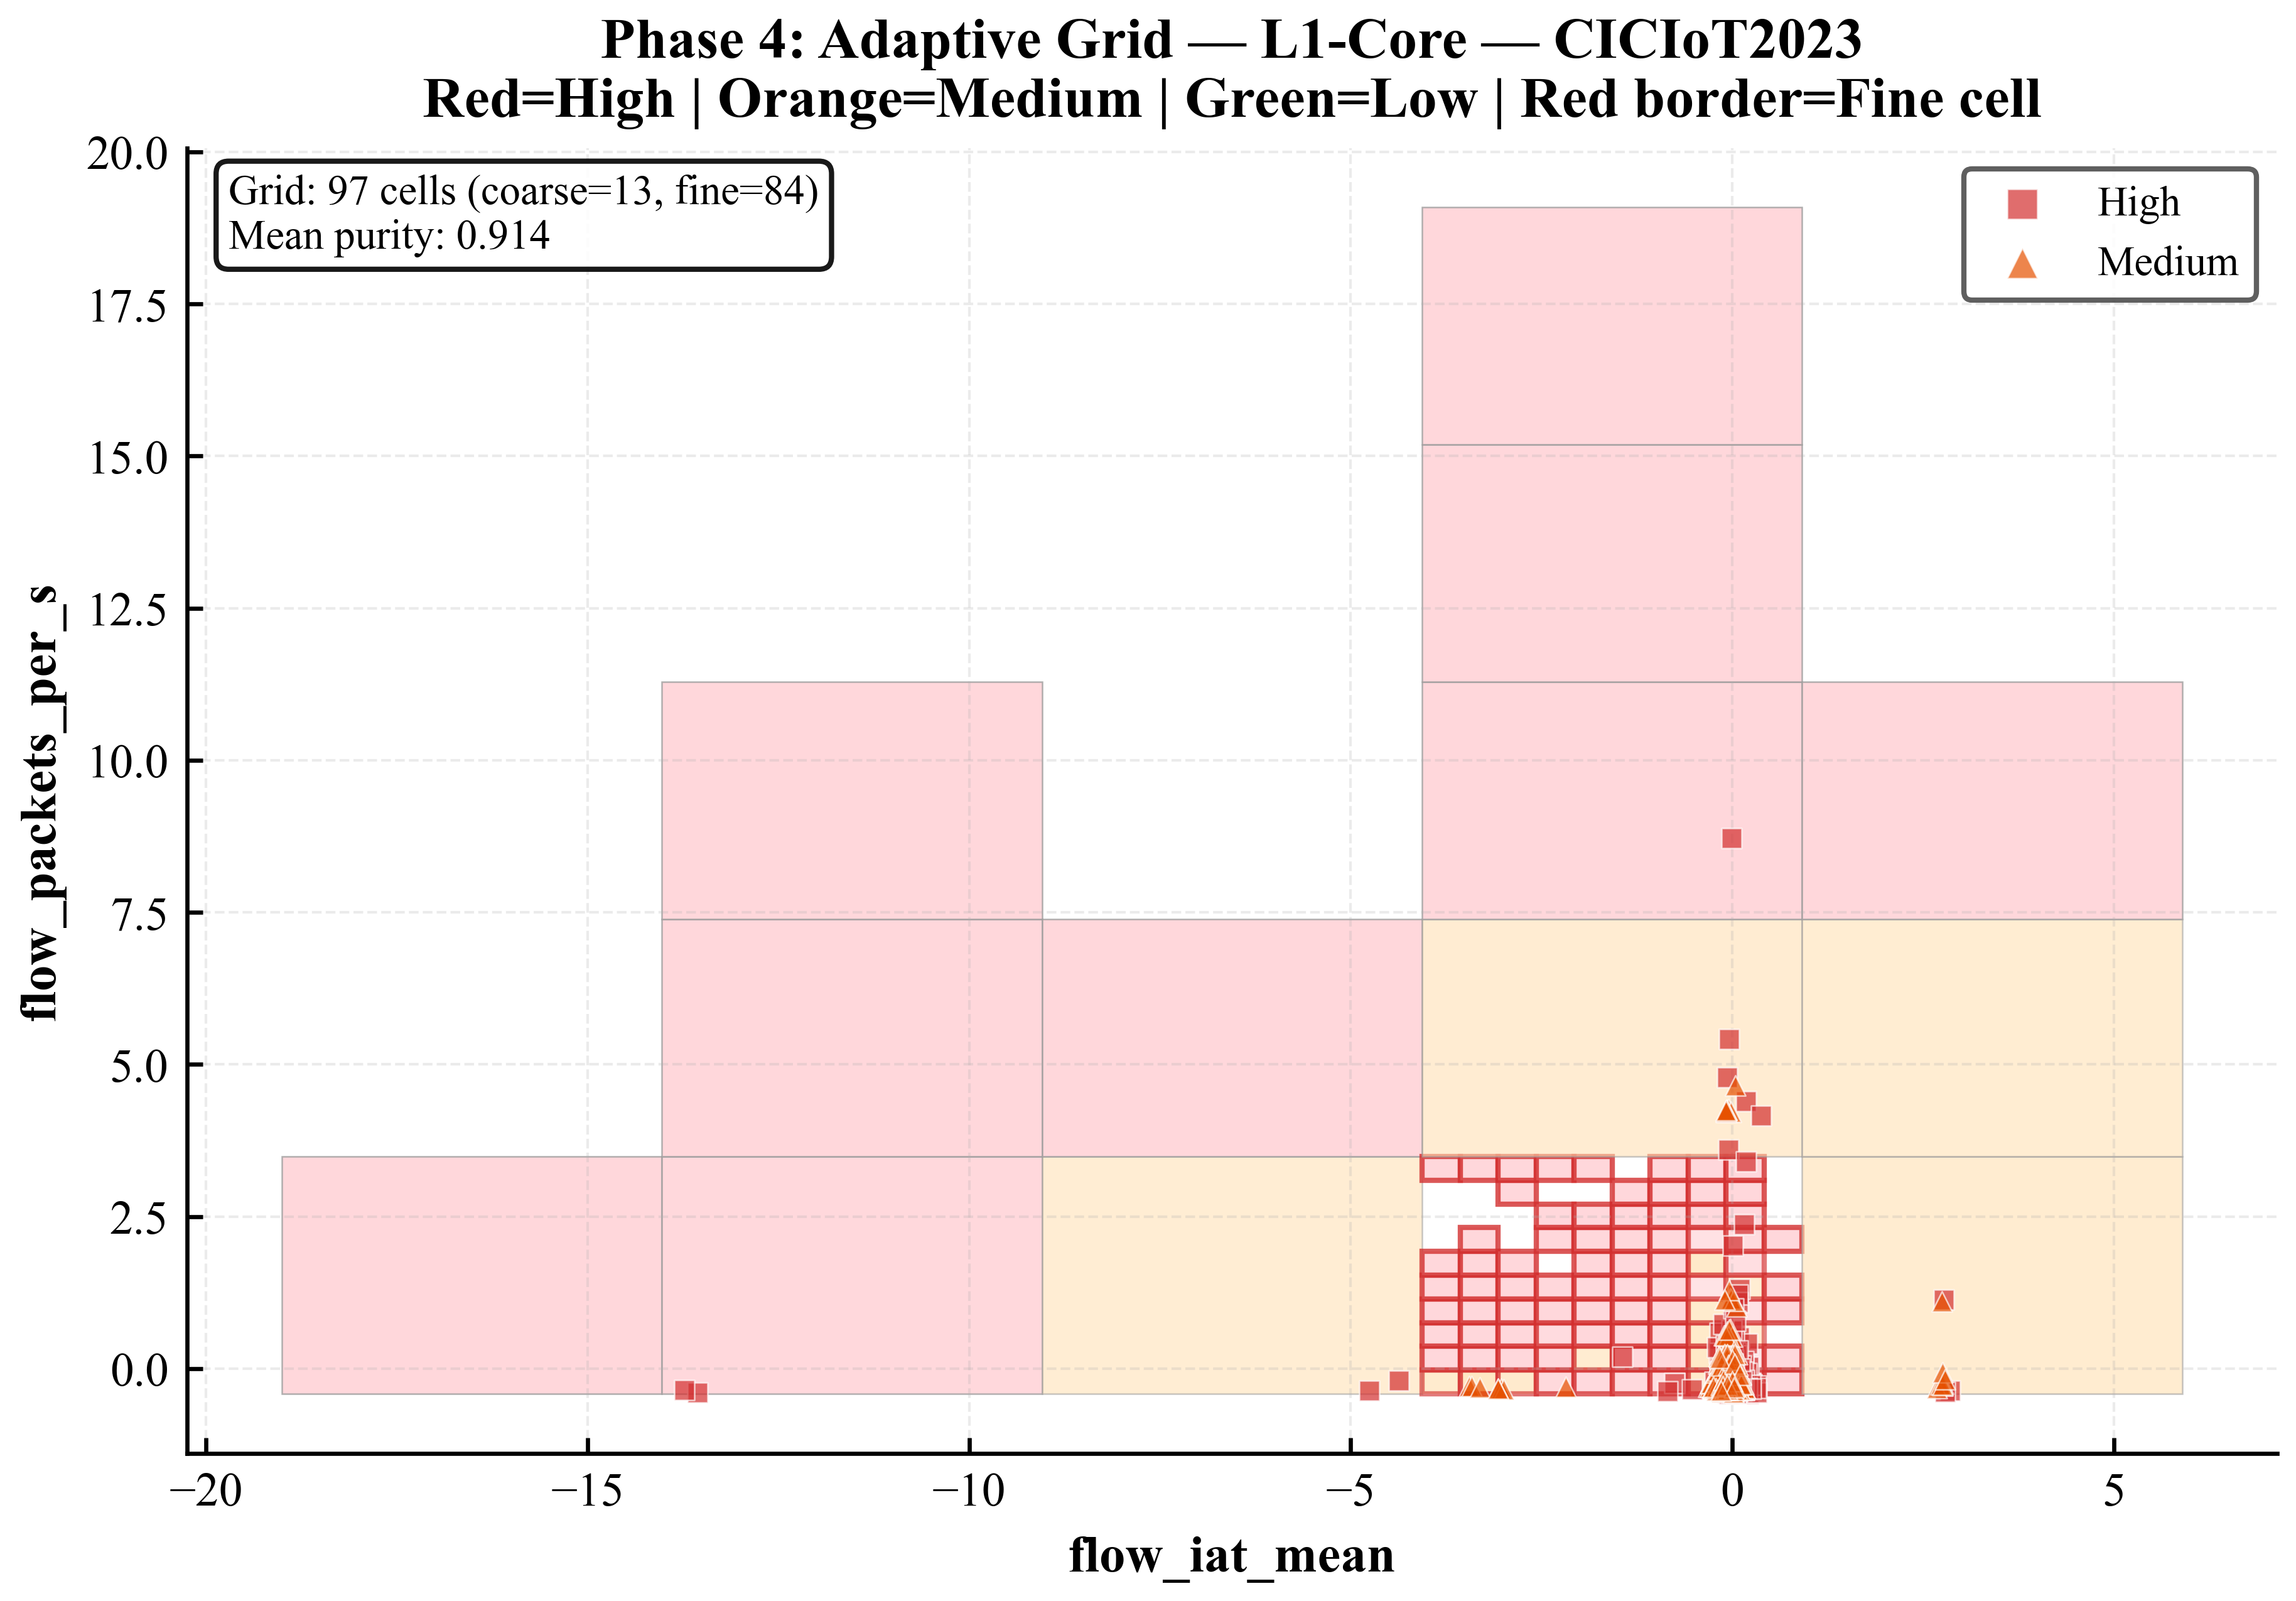
\includegraphics[width=\linewidth]{strategyB_ciciot2023/01_AFRAS_FL/fig04a_grid_L1_Core.png}
    \caption{Adaptive grid}
  \end{subfigure}
  \caption{AFRAS-FL rule mining stages on the core link (CICIoT2023): the
  signal flow is denoised, a kernel density estimate locates high-mass
  regions, and an adaptive grid produces the input cells from which fuzzy
  IF--THEN rules are generated.}\label{fig:rule_mining}
\end{figure}

Having localised where the rules come from, we can characterise
them more precisely. Fig.~\ref{fig:membership_rules} shows the fuzzy
membership functions and the resulting rule confidence/support
profile, and Fig.~\ref{fig:rule_quality} shows rule-firing heatmaps
and per-client counts. Together they establish that the extracted
rule-base is compact (typically $\le 15$ rules per agent),
high-confidence, and balanced across the five federated clients ---
the structural precondition for tracing how the trained policy
evolves across phases.

\begin{figure}[!htbp]
  \centering
  \begin{subfigure}{0.48\linewidth}
    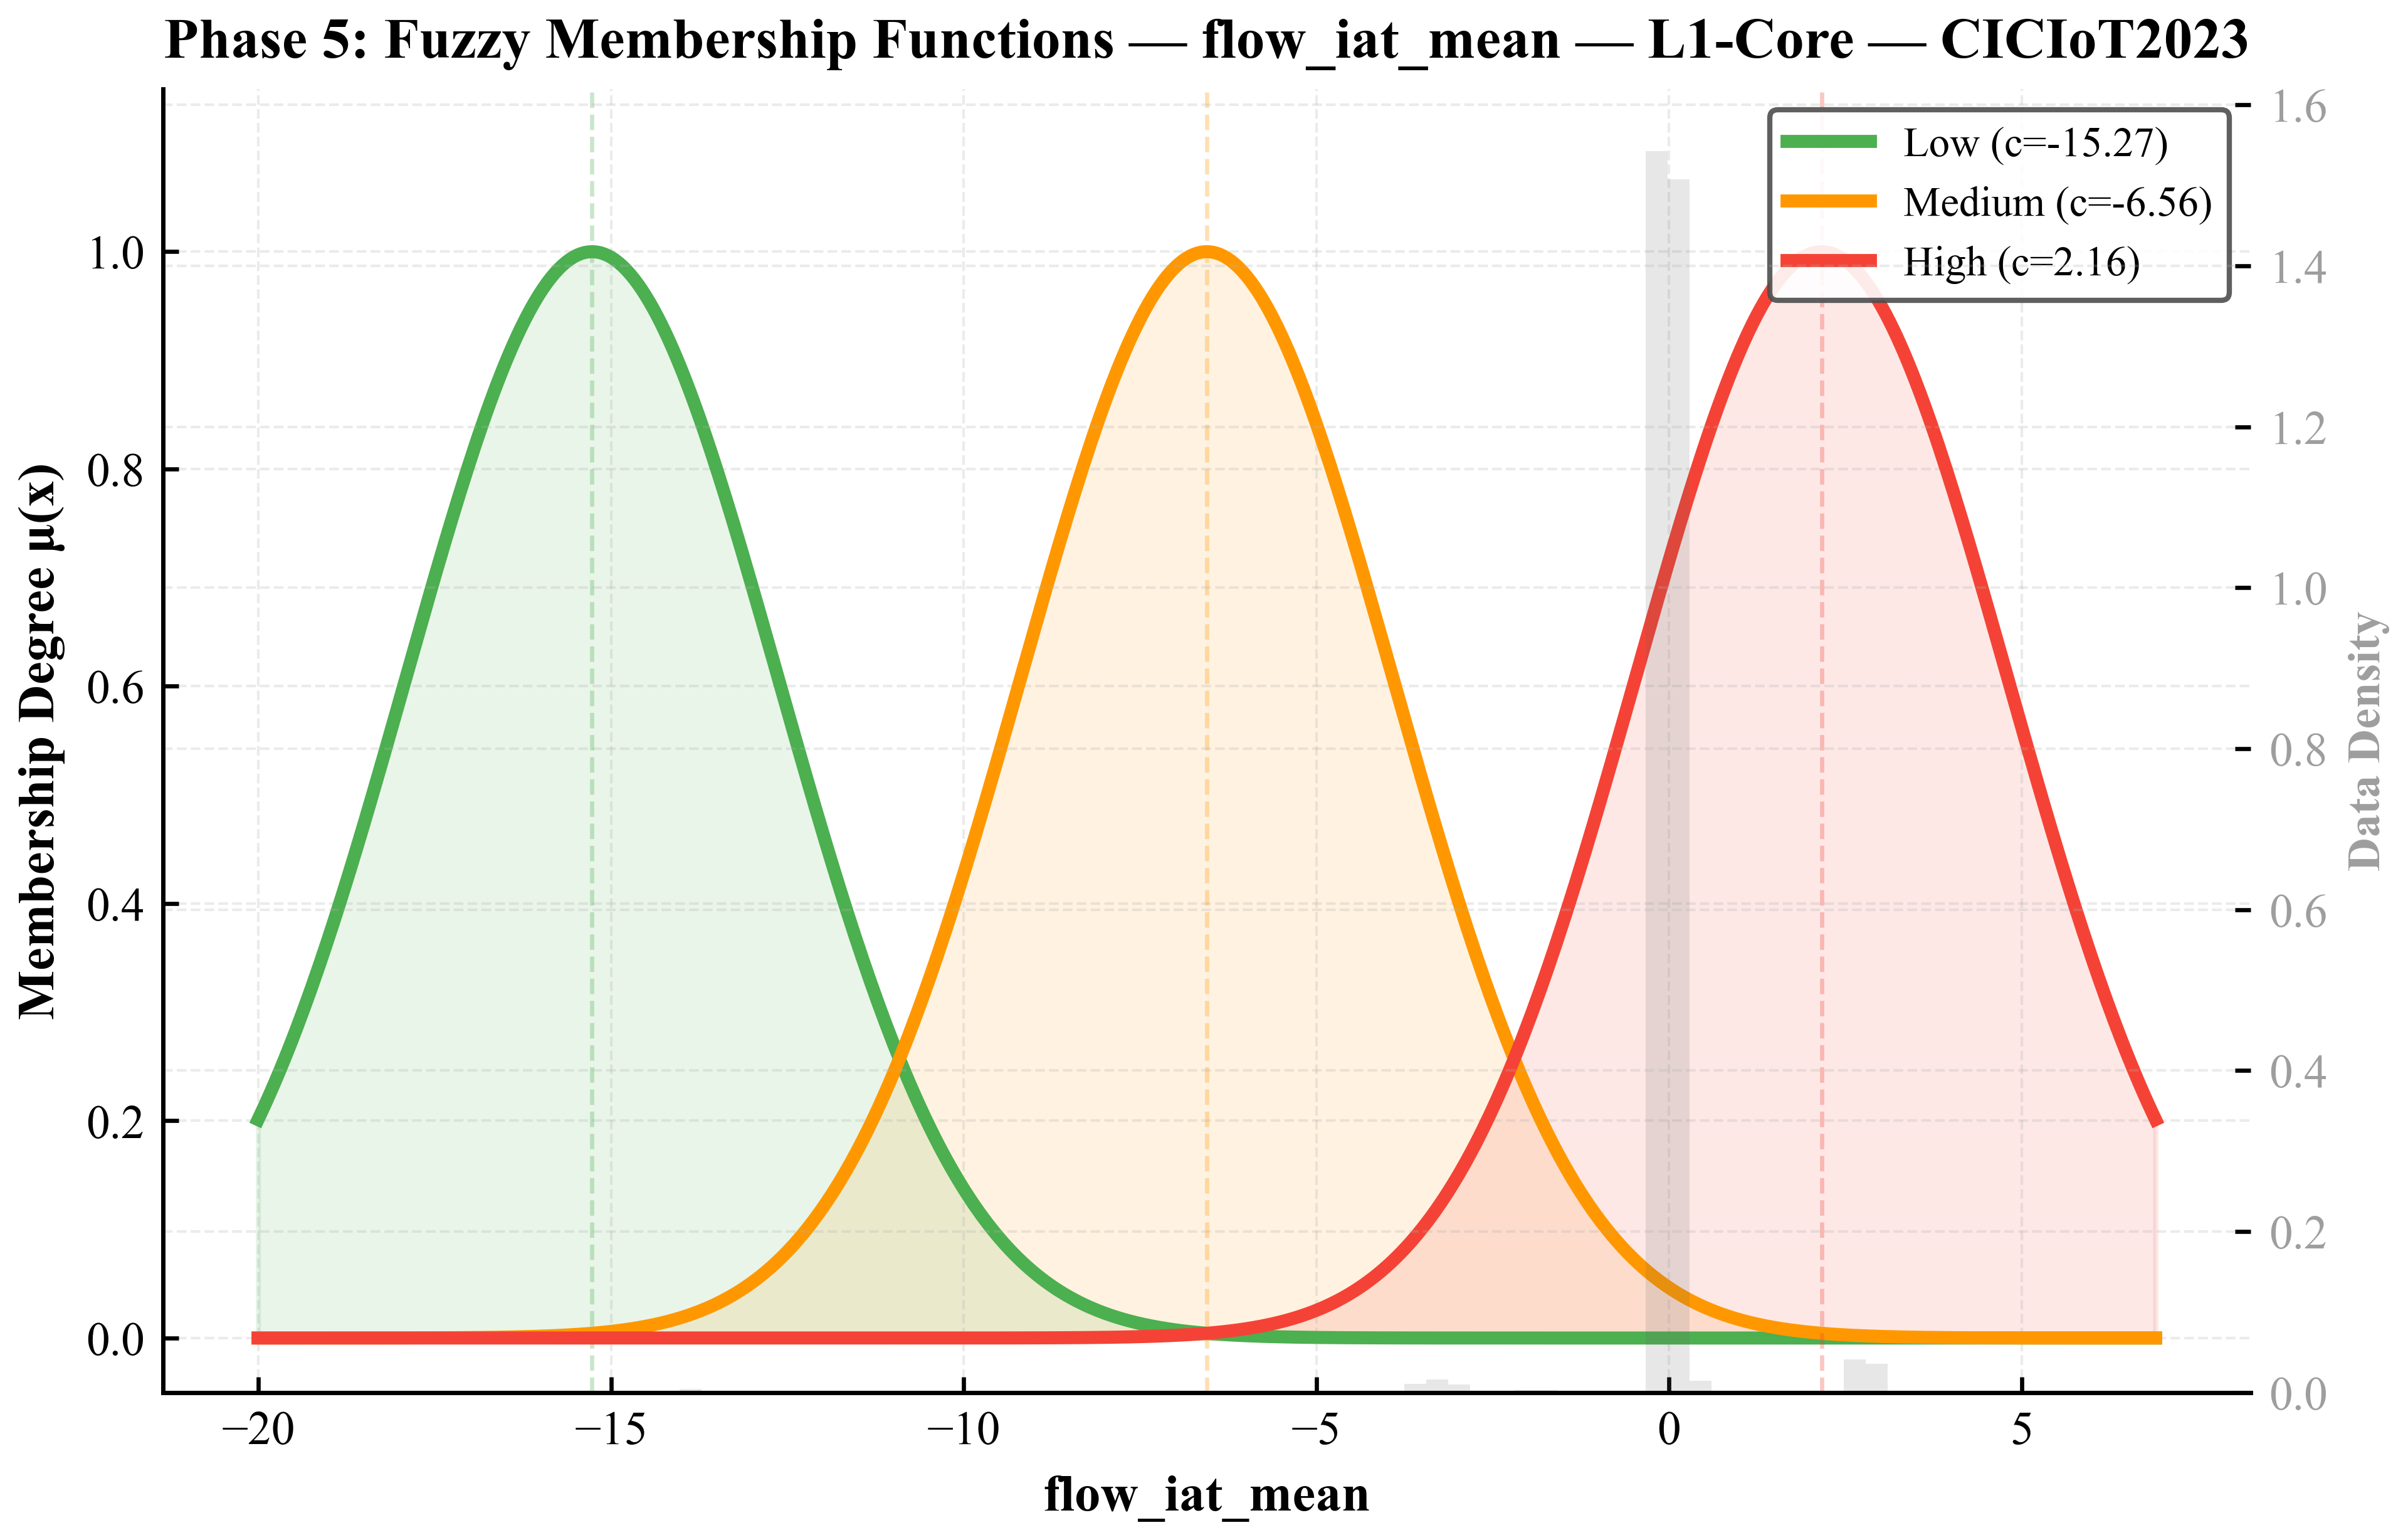
\includegraphics[width=\linewidth]{strategyB_ciciot2023/01_AFRAS_FL/fig05_membership_flow_iat_mean_L1_Core.png}
    \caption{Fuzzy membership functions for inter-arrival time}
  \end{subfigure}
  \hfill
  \begin{subfigure}{0.48\linewidth}
    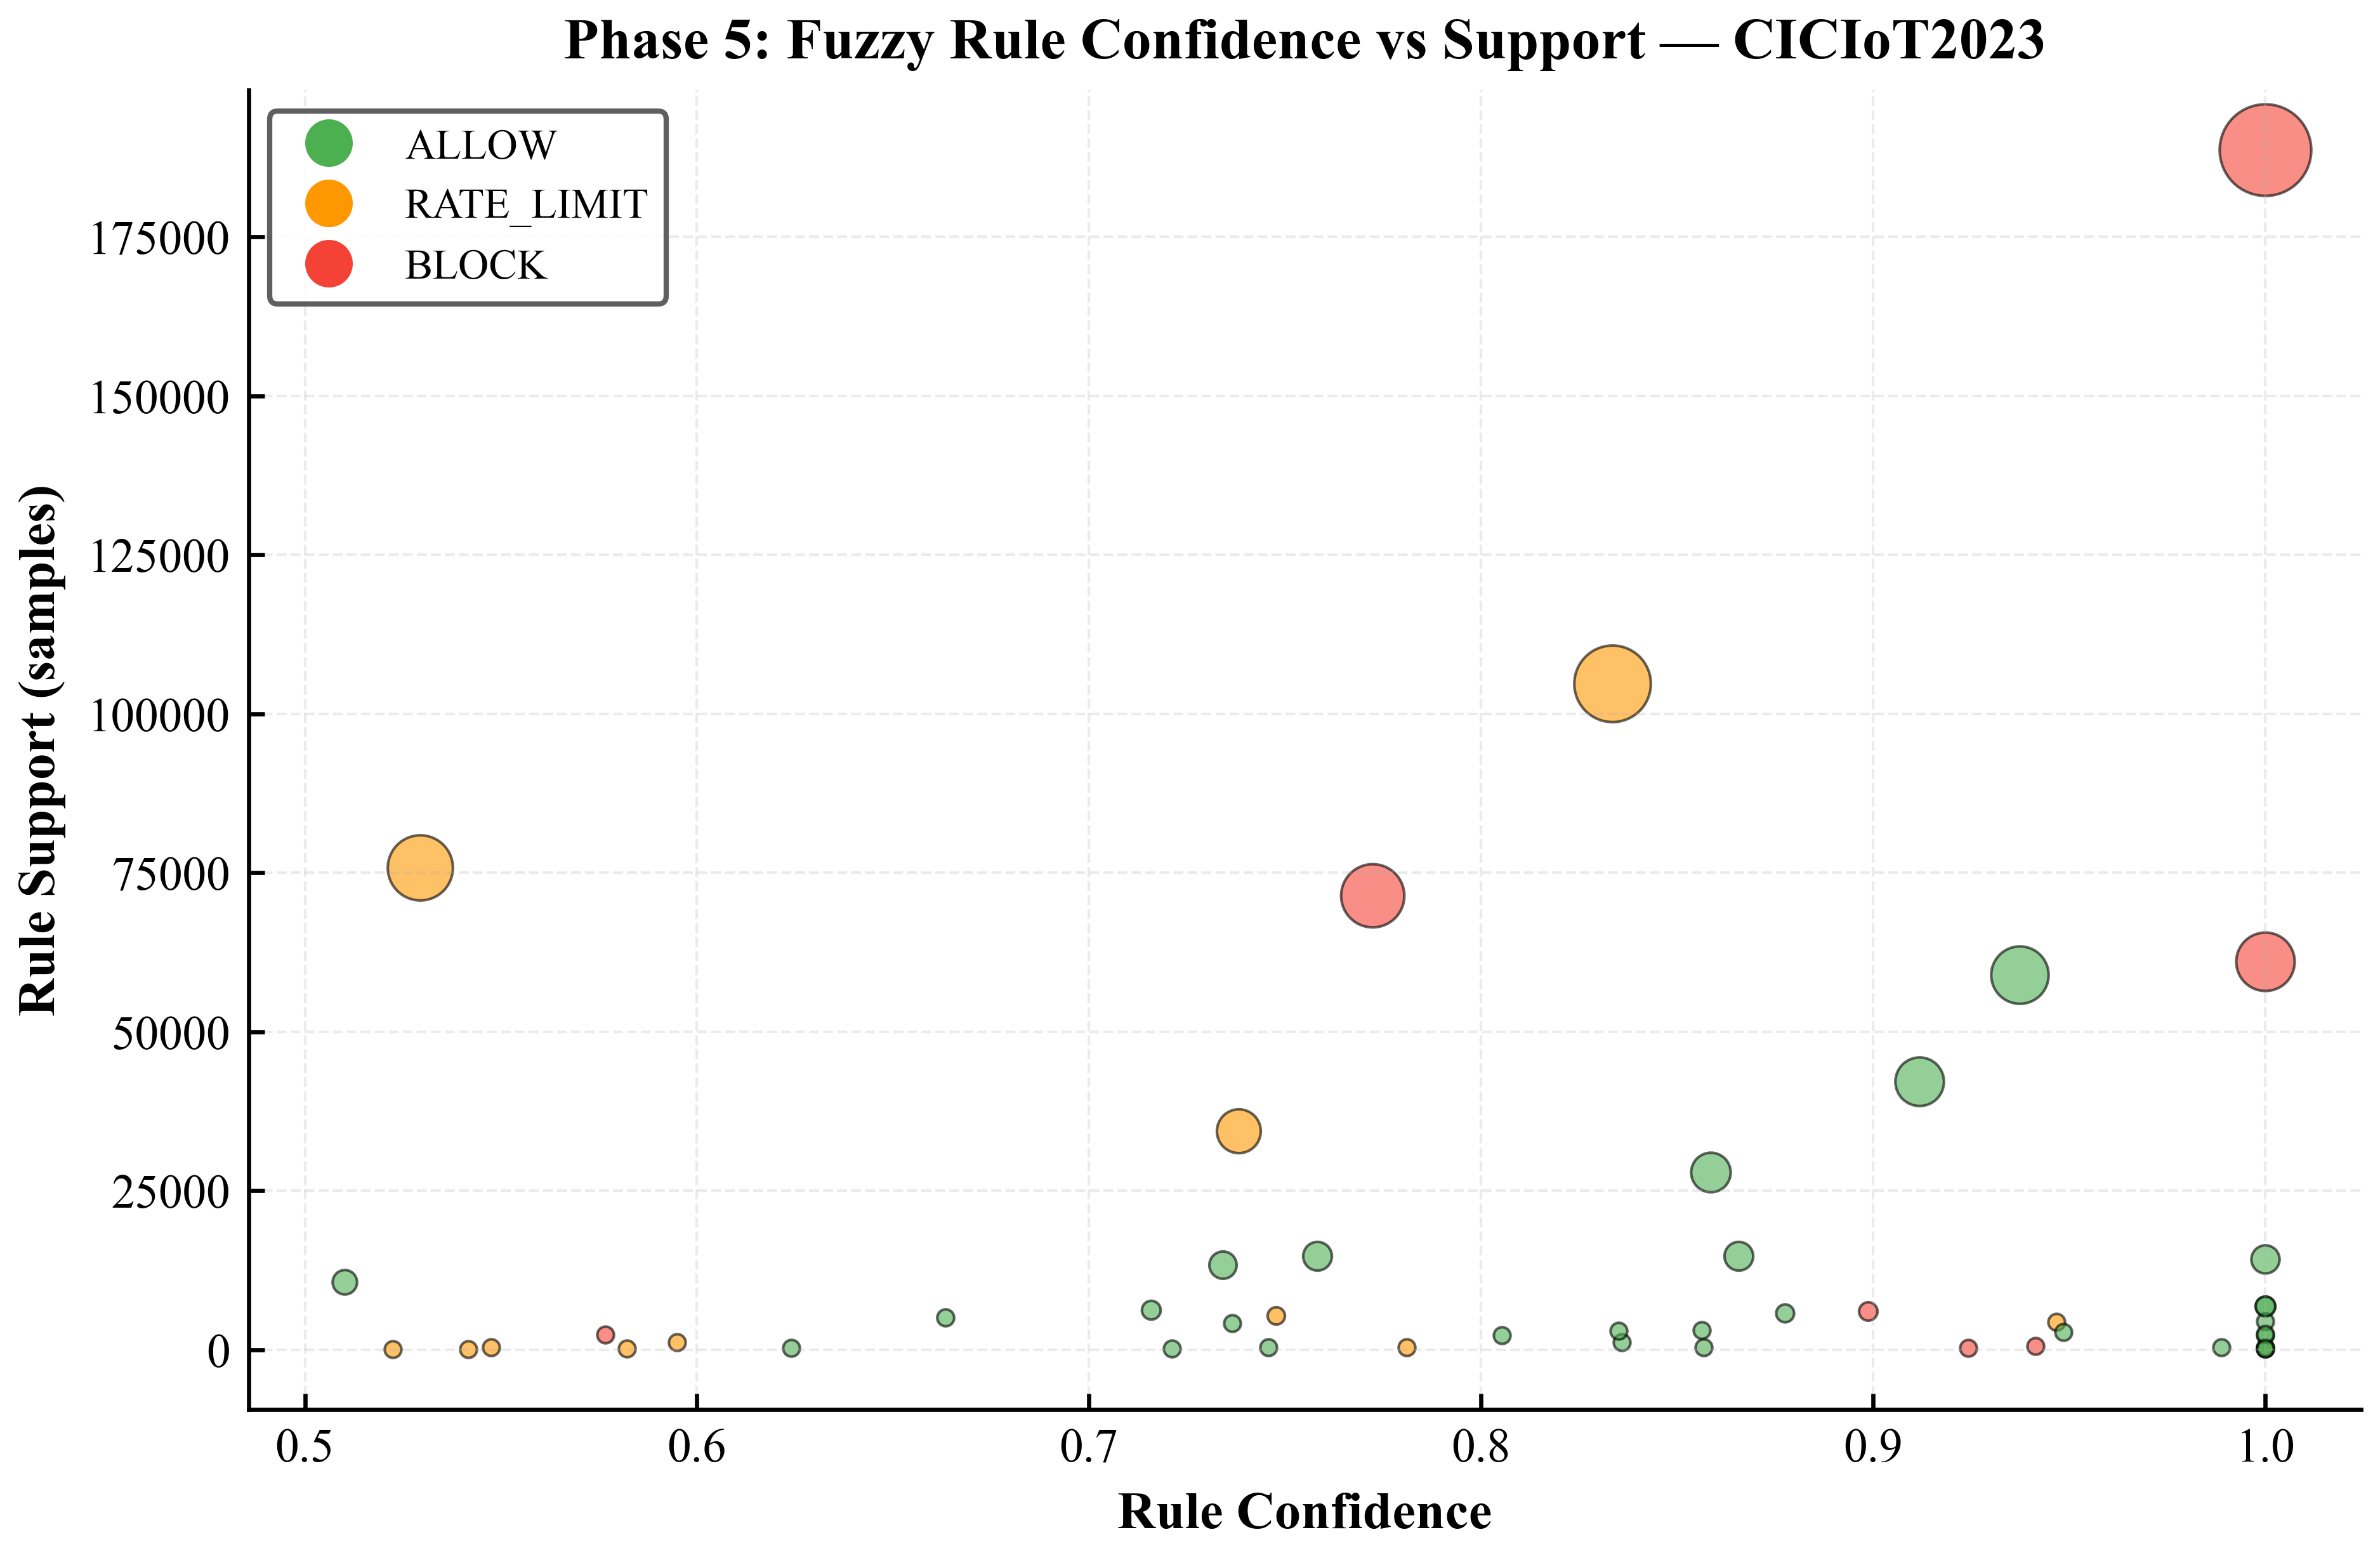
\includegraphics[width=\linewidth]{strategyB_ciciot2023/01_AFRAS_FL/fig06_rule_confidence_support.png}
    \caption{Rule confidence vs.\ support}
  \end{subfigure}
  \caption{Membership functions and the confidence--support distribution
  of the extracted fuzzy rules on the core link of CICIoT2023.}
  \label{fig:membership_rules}
\end{figure}

\begin{figure}[!htbp]
  \centering
  \begin{subfigure}{0.32\linewidth}
    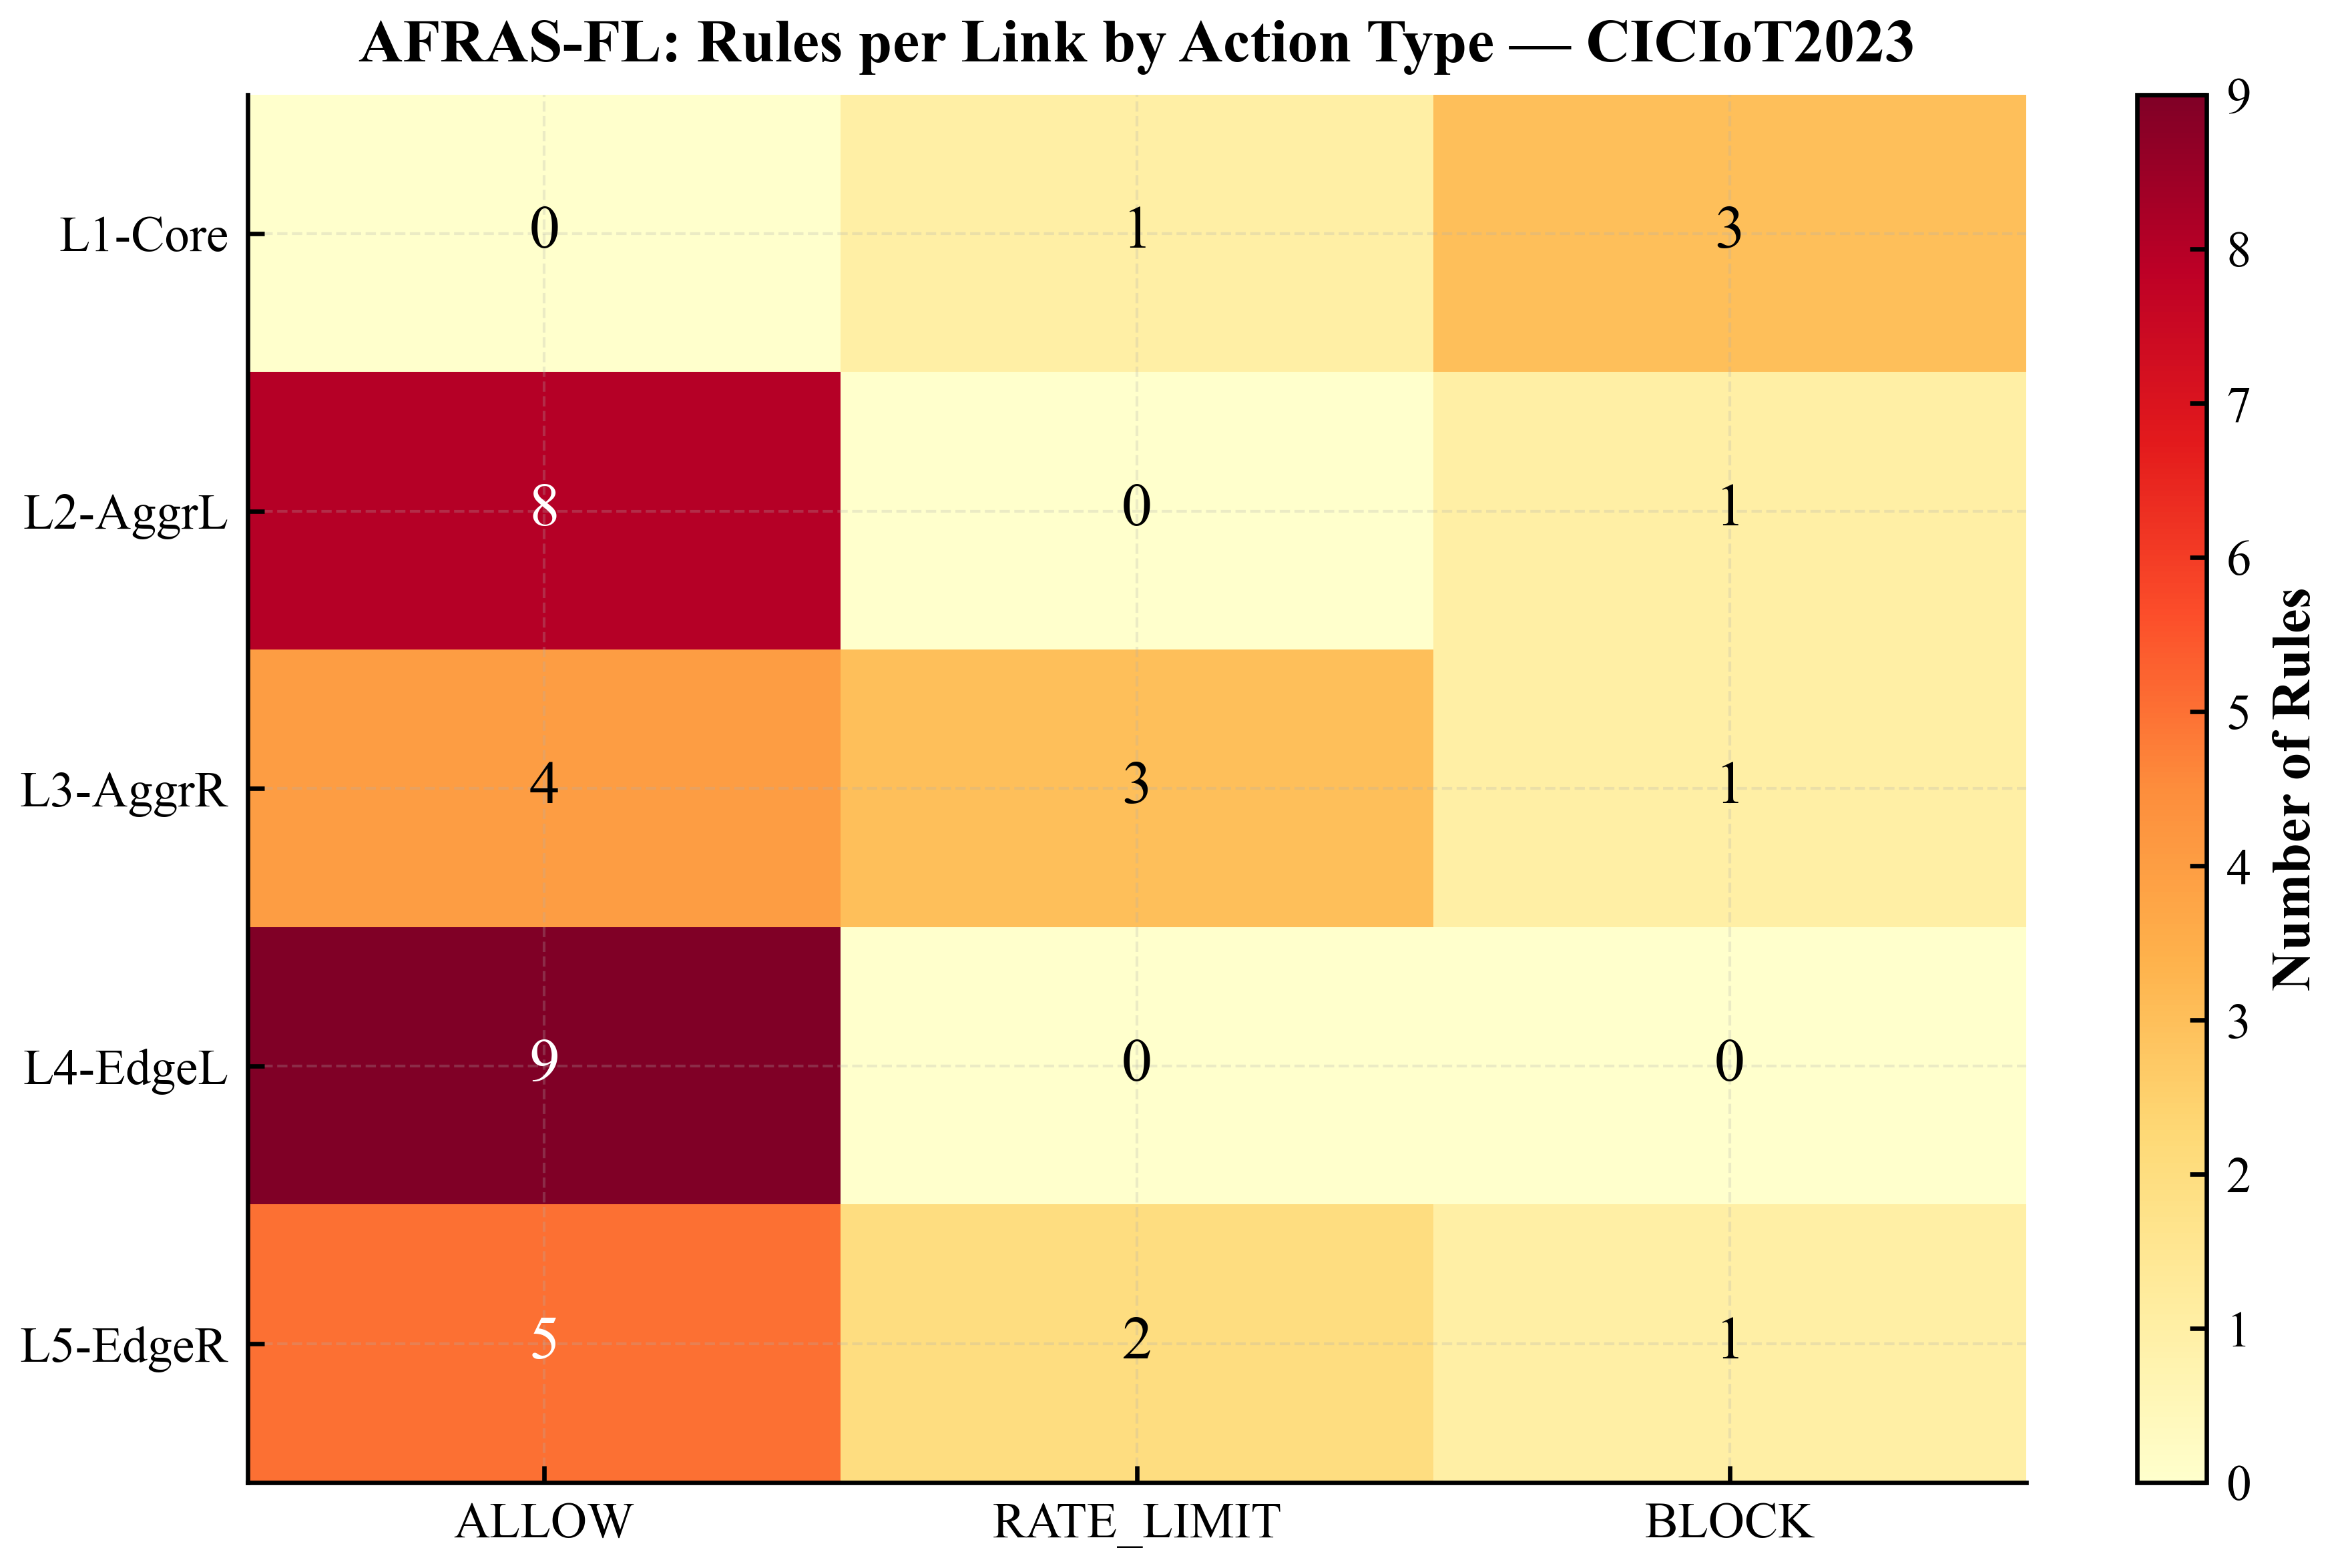
\includegraphics[width=\linewidth]{strategyB_ciciot2023/01_AFRAS_FL/fig08_rules_heatmap.png}
    \caption{Rule-firing heatmap}
  \end{subfigure}
  \hfill
  \begin{subfigure}{0.32\linewidth}
    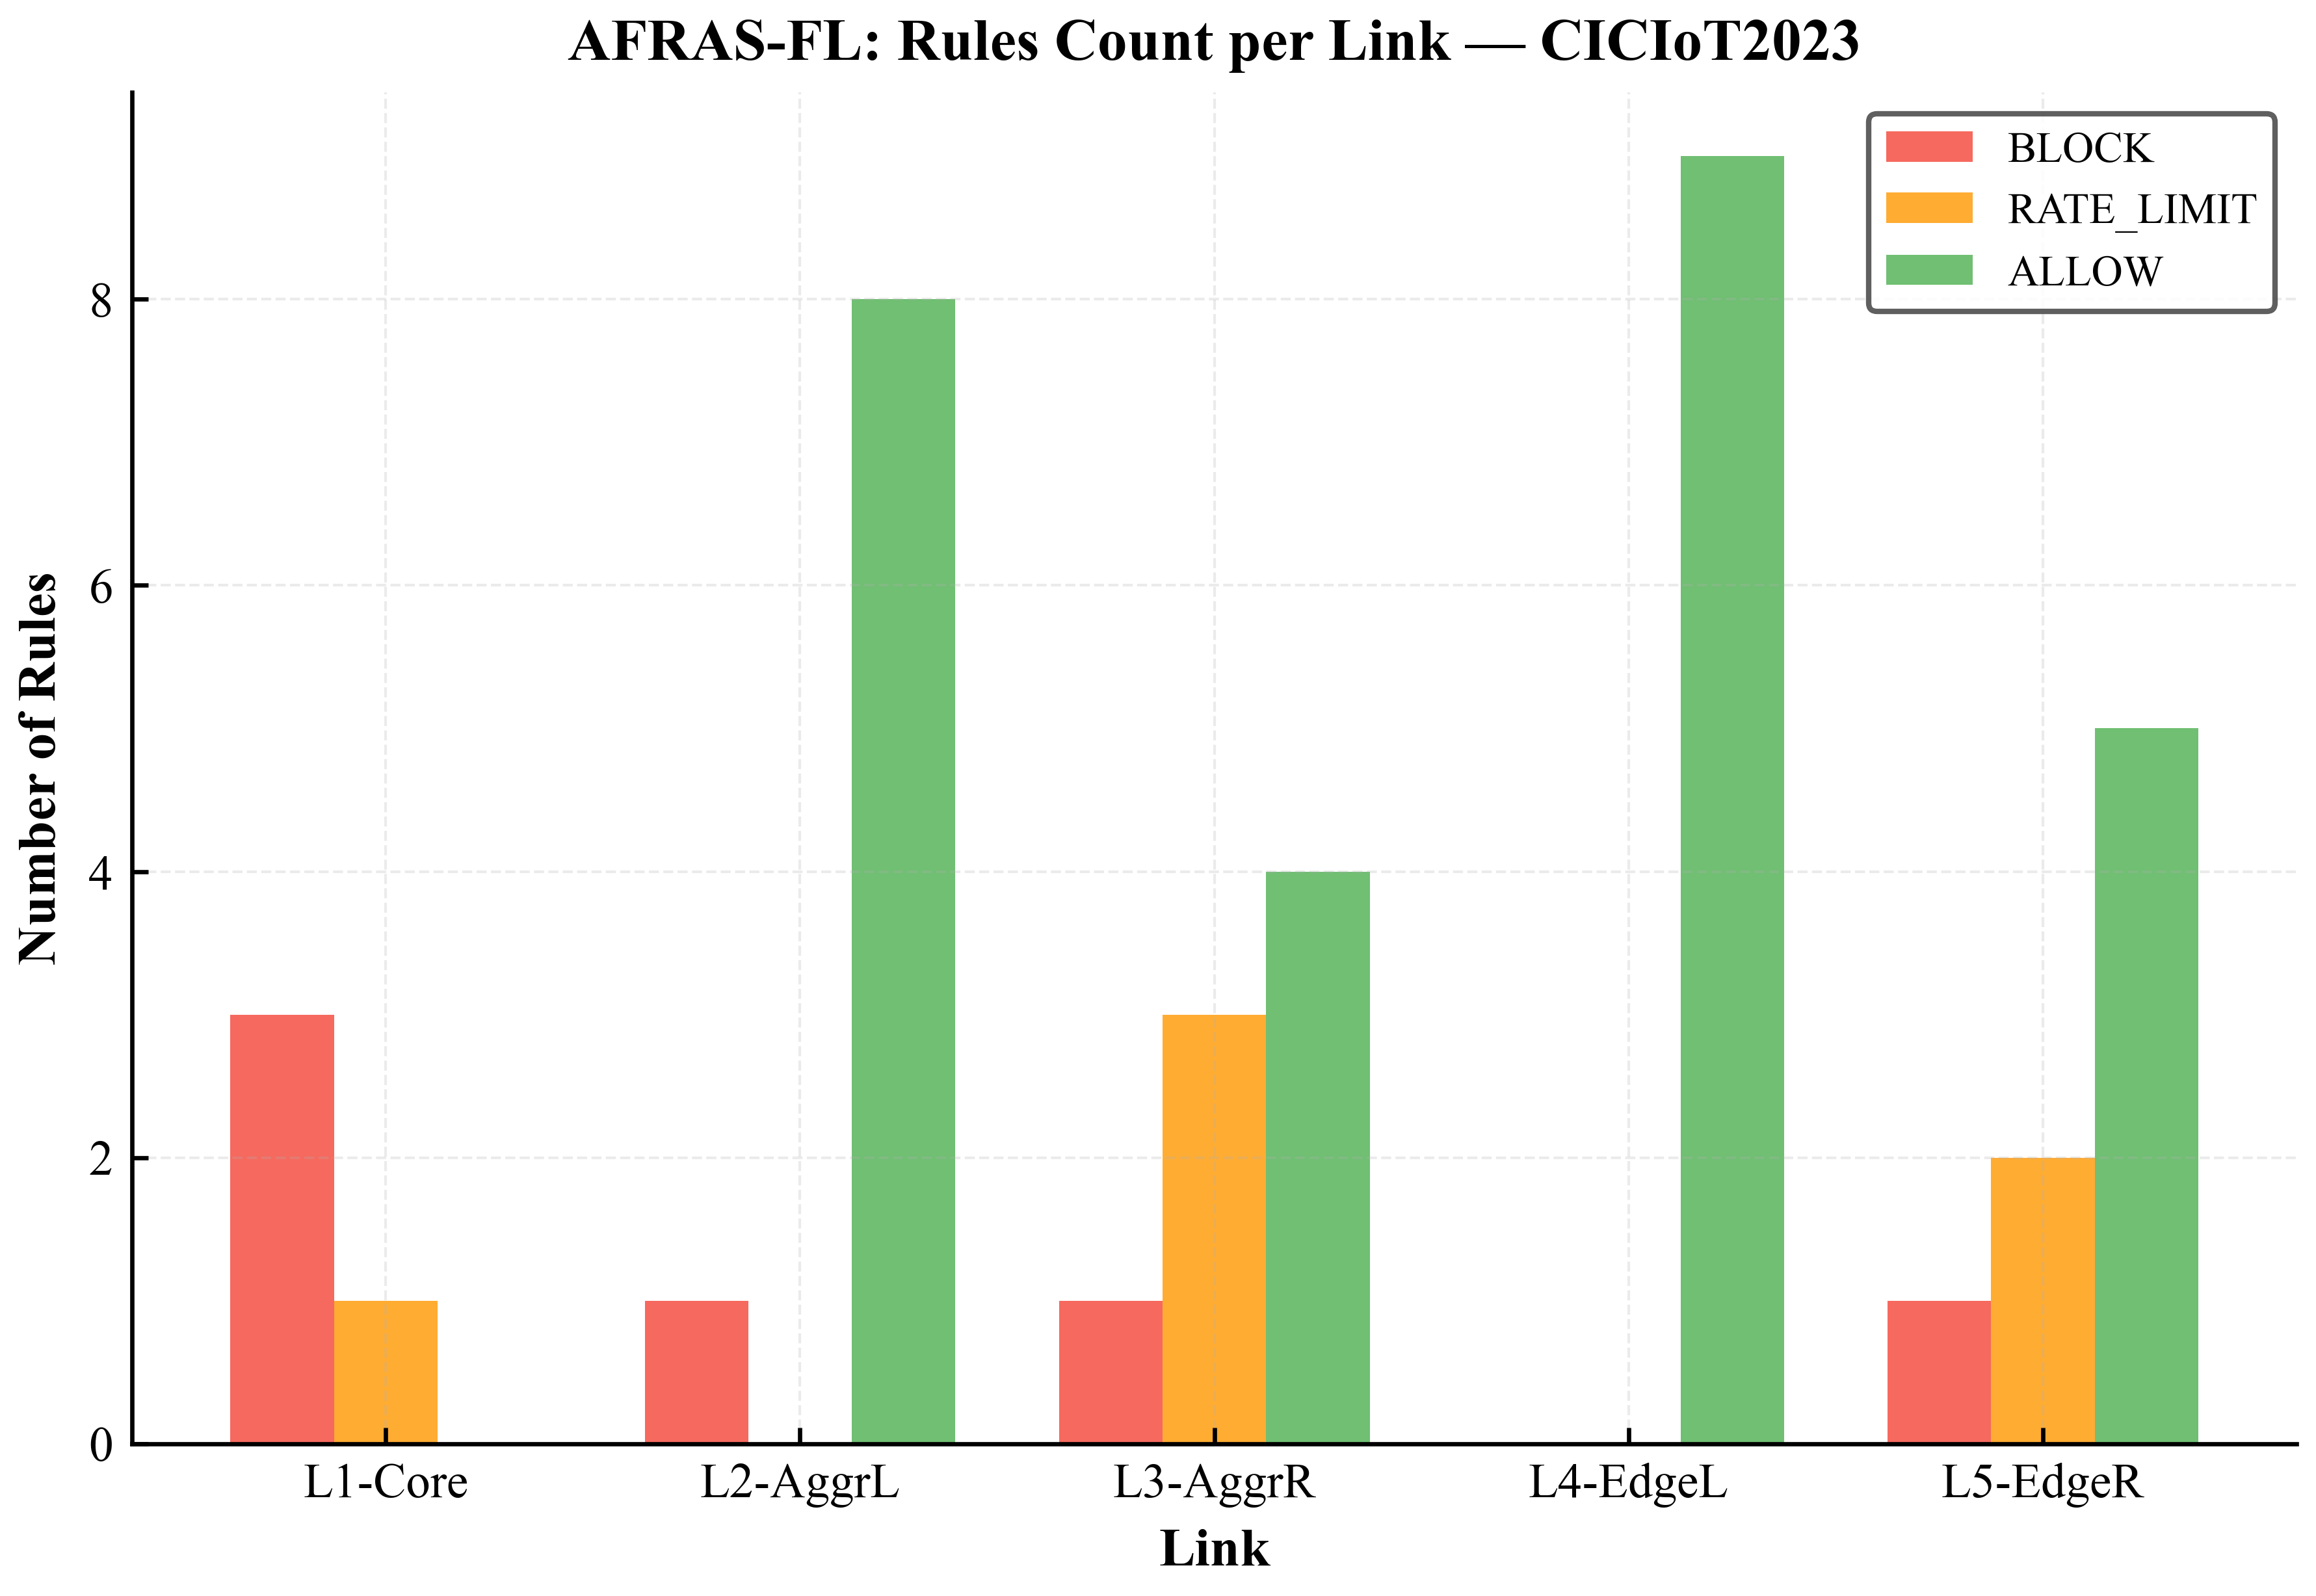
\includegraphics[width=\linewidth]{strategyB_ciciot2023/01_AFRAS_FL/fig09_afras_rules_count.png}
    \caption{Rules per client}
  \end{subfigure}
  \hfill
  \begin{subfigure}{0.32\linewidth}
    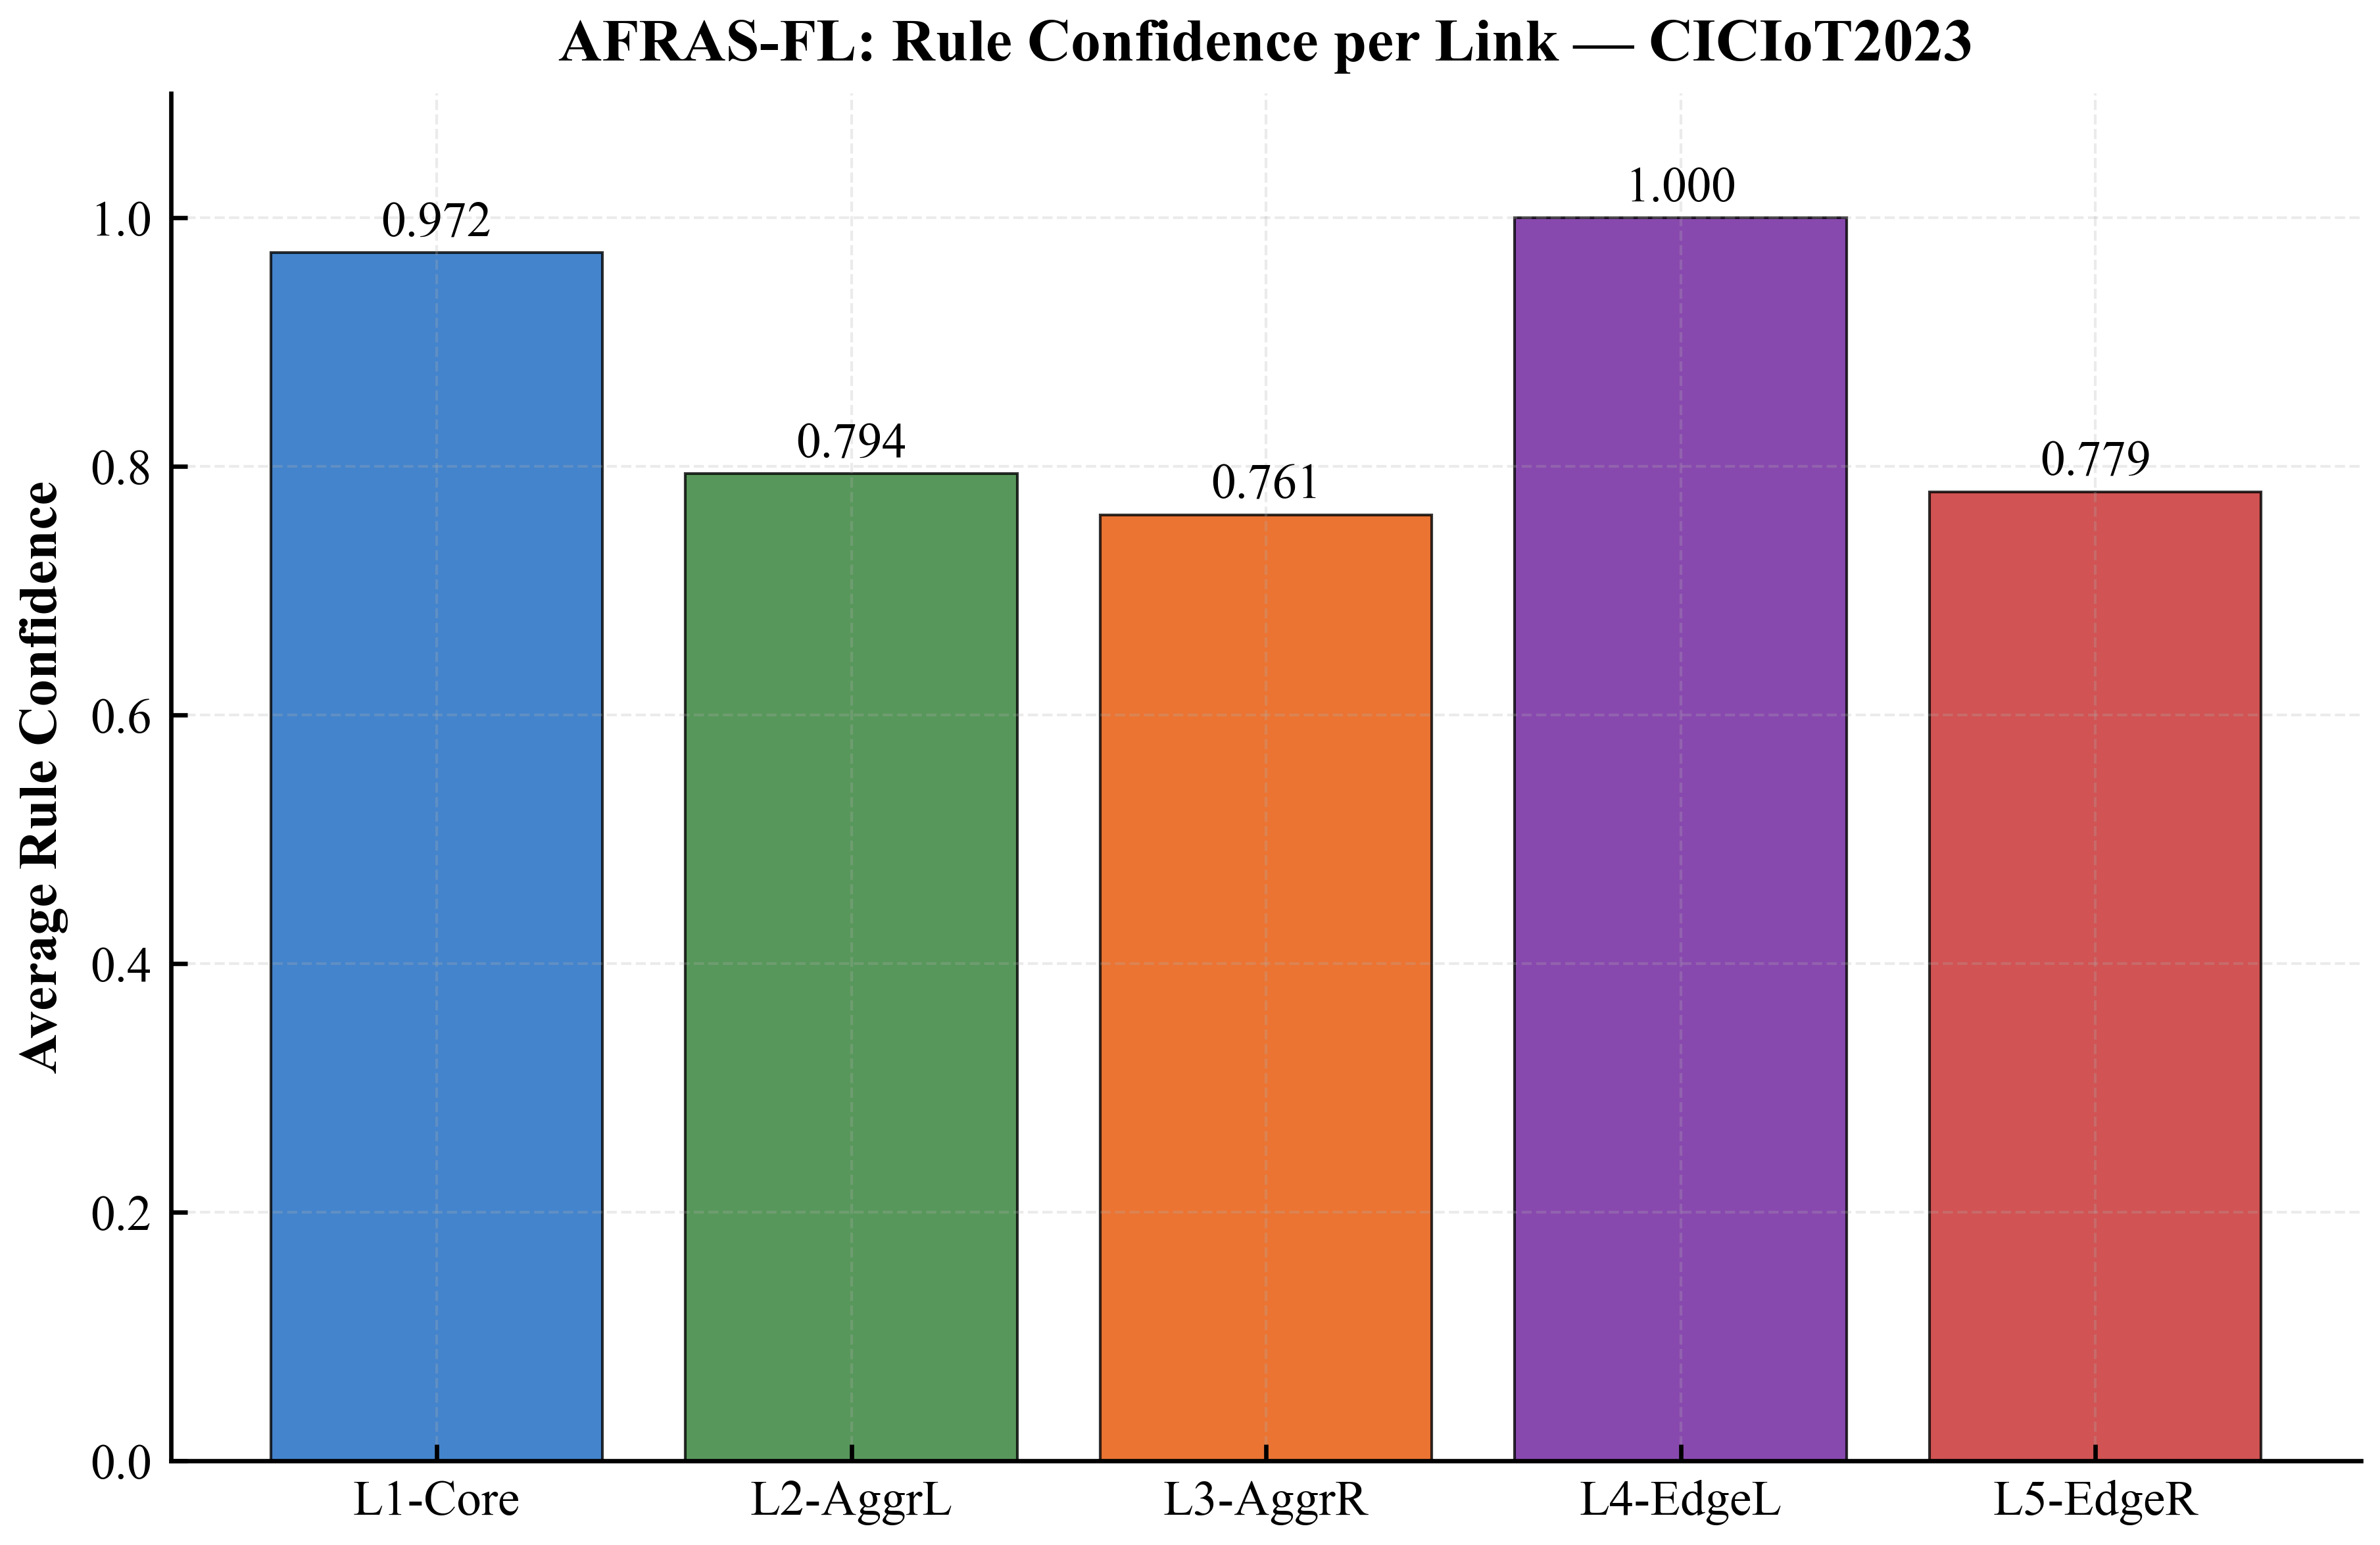
\includegraphics[width=\linewidth]{strategyB_ciciot2023/01_AFRAS_FL/fig10_afras_confidence.png}
    \caption{Confidence distribution}
  \end{subfigure}
  \caption{Quality of the extracted fuzzy rule-base across the five
  non-IID clients of CICIoT2023.}\label{fig:rule_quality}
\end{figure}

% ----------------------------------------------------------------------------
\subsection{Phase-by-phase improvement is monotone on CICIoT2023 and
graceful on DIAD2024}\label{sec:r3_phases}

With that compact rule-base in hand, we can track how the federated
agent behaves as more of the shared structure is switched on.
Training is organised into five phases: B0 (rule extraction
baseline), B1 (independent local training), B2 (FedAvg), B3
(FedProx), and B4 (full fuzzy-augmented federated training).
Table~\ref{tab:phase_msr} reports the Mean Success Rate (MSR), Jain
Fairness Index (JFI), false-positive rate (FPR), false-negative
rate (FNR), and mean reward across all five phases on both
datasets.

\begin{table*}[!htbp]
  \centering
  \caption{Phase-by-phase performance of the fuzzy-augmented federated
  DRL agent across the two benchmarks. MSR: Mean Success Rate; JFI: Jain
  Fairness Index; FPR: False-Positive Rate; FNR: False-Negative Rate.
  Numbers are averaged over 50 evaluation episodes. \rev{Bold marks the best \emph{federated} phase (B2--B4) per column, computed independently for each metric. On CICIoT2023, phase B4 dominates. On DIAD2024, phase B2 (FedAvg) is best on MSR, JFI, FNR, and Reward, while phase B3 (FedProx) is best on FPR; B4 (fuzzy-augmented) is not the best federated phase on any metric --- see Section~\ref{sec:r6_envelope} for the operational-envelope discussion.}}\label{tab:phase_msr}
  \small
  \begin{tabular}{@{}llccccc@{}}
    \toprule
    \textbf{Dataset} & \textbf{Phase} & \textbf{MSR} & \textbf{JFI} & \textbf{FPR} & \textbf{FNR} & \textbf{Reward} \\
    \midrule
    \multirow{4}{*}{CICIoT2023}
      & B1 (Local)   & $0.9985\pm0.0018$ & $1.0000$ & $0.0004$ & $0.0000$ & $0.566$ \\
      & B2 (FedAvg)  & $0.9817\pm0.0147$ & $0.9998$ & $0.0199$ & $0.0008$ & $0.556$ \\
      & B3 (FedProx) & $0.9978\pm0.0028$ & $1.0000$ & $0.0036$ & $0.0053$ & $0.565$ \\
      & B4 (Fuzzy)   & $\mathbf{0.9990\pm0.0010}$ & $\mathbf{1.0000}$ & $\mathbf{0.0026}$ & $\mathbf{0.0001}$ & $0.554$ \\
    \midrule
    \multirow{4}{*}{DIAD2024}
      & B1 (Local)   & $0.9996\pm0.0004$ & $1.0000$ & $0.0001$ & $0.0000$ & $0.506$ \\
      & B2 (FedAvg)  & \rev{$\mathbf{0.9318\pm0.0565}$} & \rev{$\mathbf{0.9963}$} & $0.2000$ & \rev{$\mathbf{0.0002}$} & \rev{$\mathbf{0.470}$} \\
      & B3 (FedProx) & \rev{$0.9028\pm0.1036$} & \rev{$0.9870$} & \rev{$\mathbf{0.0018}$} & \rev{$0.0212$} & \rev{$0.454$} \\
      & B4 (Fuzzy)   & \rev{$0.8474\pm0.1505$} & \rev{$0.9694$} & \rev{$0.0421$} & \rev{$0.0415$} & \rev{$0.414$} \\
    \bottomrule
  \end{tabular}
\end{table*}

\begin{table*}[!htbp]
  \centering
  \caption{Phase-B0 fuzzy rule statistics extracted by AFRAS-FL across the
  five non-IID clients (links L1--L5).}\label{tab:phase_b0}
  \small
  \begin{tabular}{@{}llccccc@{}}
    \toprule
    \textbf{Dataset} & \textbf{Link} & \textbf{Total} & \textbf{Block} & \textbf{Limit} & \textbf{Allow} & \textbf{Avg.\ Conf.} \\
    \midrule
    \multirow{5}{*}{CICIoT2023}
      & L1-Core  & 4 & 3 & 1 & 0 & $0.972$ \\
      & L2-AggrL & 9 & 1 & 0 & 8 & $0.794$ \\
      & L3-AggrR & 8 & 1 & 3 & 4 & $0.761$ \\
      & L4-EdgeL & 9 & 0 & 0 & 9 & $1.000$ \\
      & L5-EdgeR & 8 & 1 & 2 & 5 & $0.779$ \\
    \midrule
    \multirow{5}{*}{DIAD2024}
      & L1-Core  & 6 & 5 & 1 & 0 & $0.999$ \\
      & L2-AggrL & 6 & 5 & 1 & 0 & $1.000$ \\
      & L3-AggrR & 7 & 6 & 1 & 0 & $1.000$ \\
      & L4-EdgeL & 6 & 5 & 1 & 0 & $0.999$ \\
      & L5-EdgeR & 6 & 5 & 1 & 0 & $1.000$ \\
    \bottomrule
  \end{tabular}
\end{table*}

Reading down the CICIoT2023 rows of Table~\ref{tab:phase_msr} and
the visual summary in Fig.~\ref{fig:phase_comparison}, the
fuzzy-augmented phase (B4) attains the highest MSR ($0.9990$) and
the lowest MSR standard deviation ($\sigma = 0.0010$) among all
phases. Phase B1 (Independent) has a marginally lower FPR
($4.5 \times 10^{-4}$ vs.\ $2.6 \times 10^{-3}$) because it is
allowed to overfit to each client's local distribution without the
regularisation imposed by federation; B4 is the best \emph{federated}
phase on FPR. Welch $t$-tests against the federated baselines
(Table~\ref{tab:stats}) formalise these observations: on
CICIoT2023, B4 beats FedAvg with $t = 8.35$, $p = 5.1 \times
10^{-11}$, Cohen's $d = 1.67$ (large effect), and beats FedProx
with $t = 2.94$, $p = 4.7 \times 10^{-3}$, $d = 0.59$ (medium
effect). The standard deviation of the B4 MSR is $14.6\times$
smaller than B2 (FedAvg) and $2.8\times$ smaller than B3 (FedProx),
which echoes the variance-reduction mechanism we return to in the
Discussion.

\begin{table*}[!htbp]
  \centering
  \caption{Statistical comparison of the fuzzy-augmented phase (B4)
  against the two federated baselines (B2 and B3) on the MSR metric.
  Two-sided Welch $t$-tests with $n = 50$ evaluation episodes; Cohen's
  $d$ is computed against the pooled standard deviation. The $\sigma$
  ratio is $\sigma_{\text{baseline}}/\sigma_{\text{B4}}$.}\label{tab:stats}
  \small
  \begin{tabular}{@{}llcccc@{}}
    \toprule
    \textbf{Dataset} & \textbf{Comparison} & $t$ & $p$-value & \textbf{Cohen's $d$} & $\sigma$ \textbf{ratio} \\
    \midrule
    \multirow{2}{*}{CICIoT2023}
      & B4 vs.\ FedAvg (B2)  & $+8.35$ & $5.1 \times 10^{-11}$ & $+1.67$ & $14.6\times$ \\
      & B4 vs.\ FedProx (B3) & $+2.94$ & $4.7 \times 10^{-3}$  & $+0.59$ & $2.8\times$ \\
    \midrule
    \multirow{2}{*}{DIAD2024}
      & B4 vs.\ FedAvg (B2)  & $-3.71$ & $4.4 \times 10^{-4}$  & $-0.74$ & $0.38\times^{\ast}$ \\
      & B4 vs.\ FedProx (B3) & $-2.14$ & $3.5 \times 10^{-2}$  & $-0.43$ & $0.69\times^{\ast}$ \\
    \bottomrule
  \end{tabular}

  \vspace{0.25em}
  {\footnotesize $^{\ast}$On DIAD2024, B4 has a \emph{larger} standard
  deviation than B2 and B3 because the shared fuzzy prior forces all five
  clients to converge towards a common rule-base, which increases the
  per-client residual variance on a dataset with aggressive client drift.
  See the discussion of the operational envelope below.}
\end{table*}

The DIAD2024 rows of the same table tell a different story that we
deliberately defer to R6, where the baseline comparison makes the
mechanism behind the gap explicit. The CICIoT2023 picture we just
described would be misleading, however, if it hung on a particular
value of $\lambda$; R3.1 rules that possibility out.

\begin{figure}[!htbp]
  \centering
  \begin{subfigure}{0.24\linewidth}
    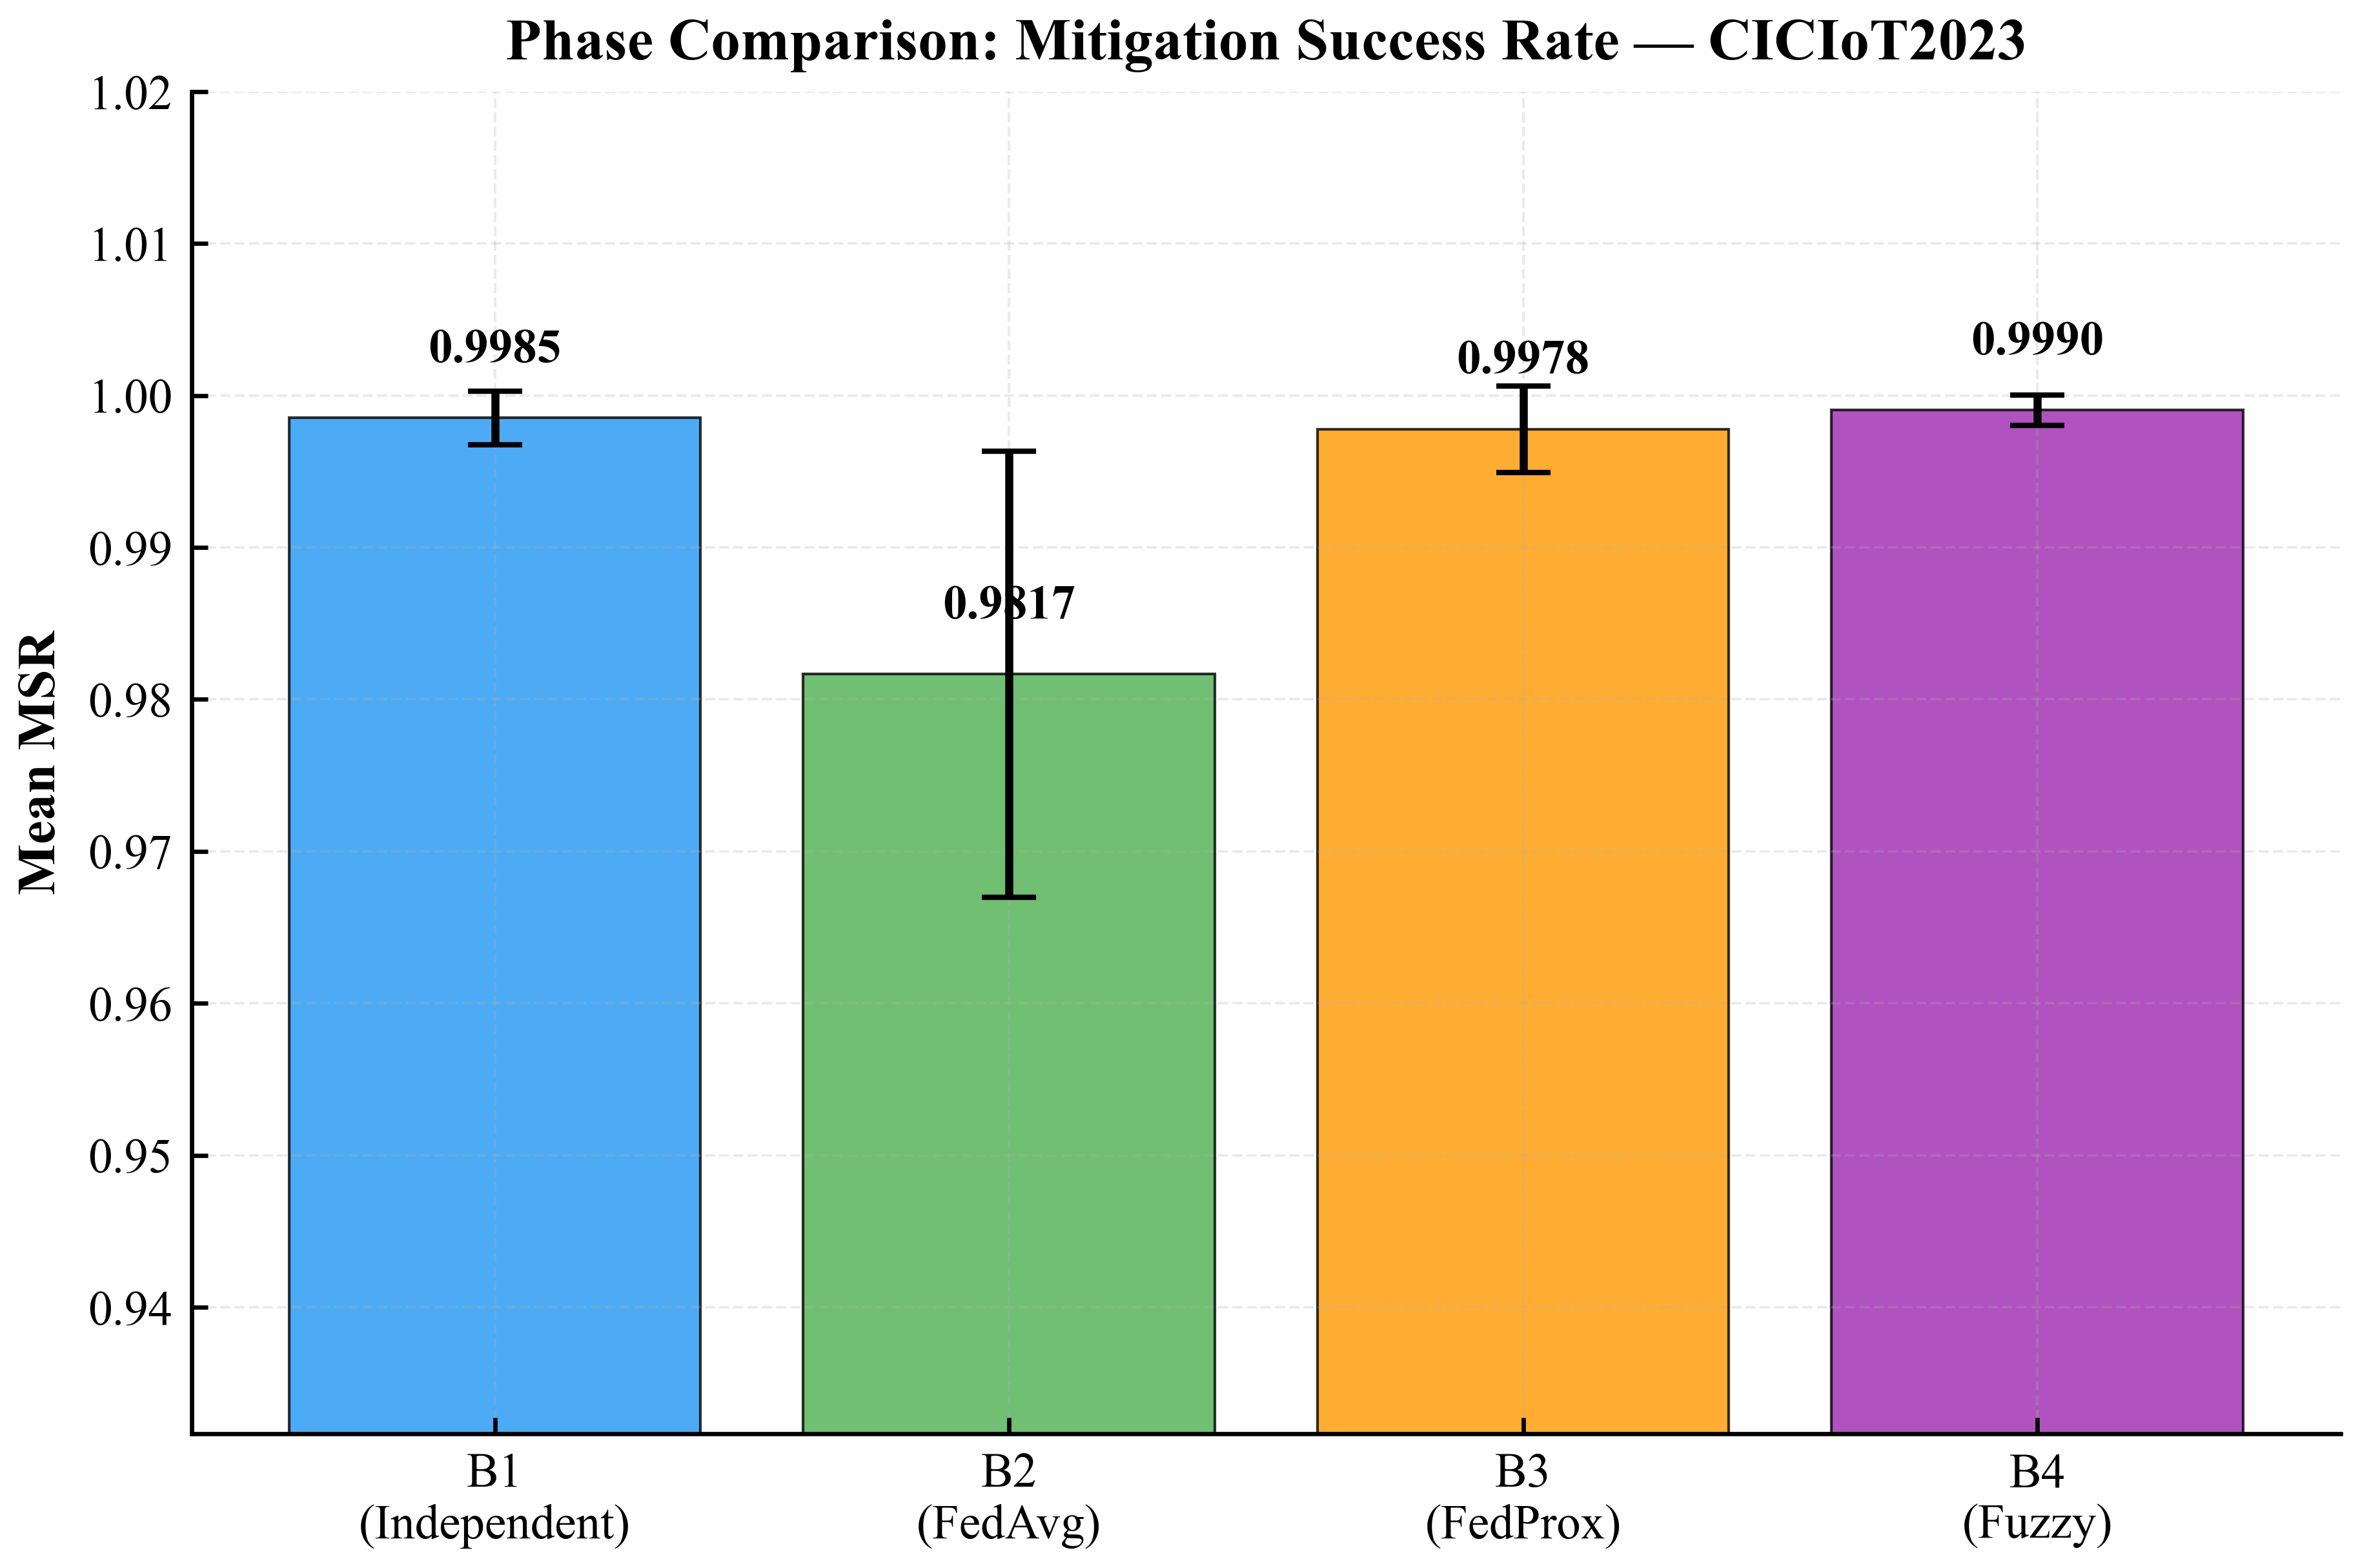
\includegraphics[width=\linewidth]{strategyB_ciciot2023/05_Phase_Comparison/fig16_phase_msr.png}
    \caption{MSR}
  \end{subfigure}
  \hfill
  \begin{subfigure}{0.24\linewidth}
    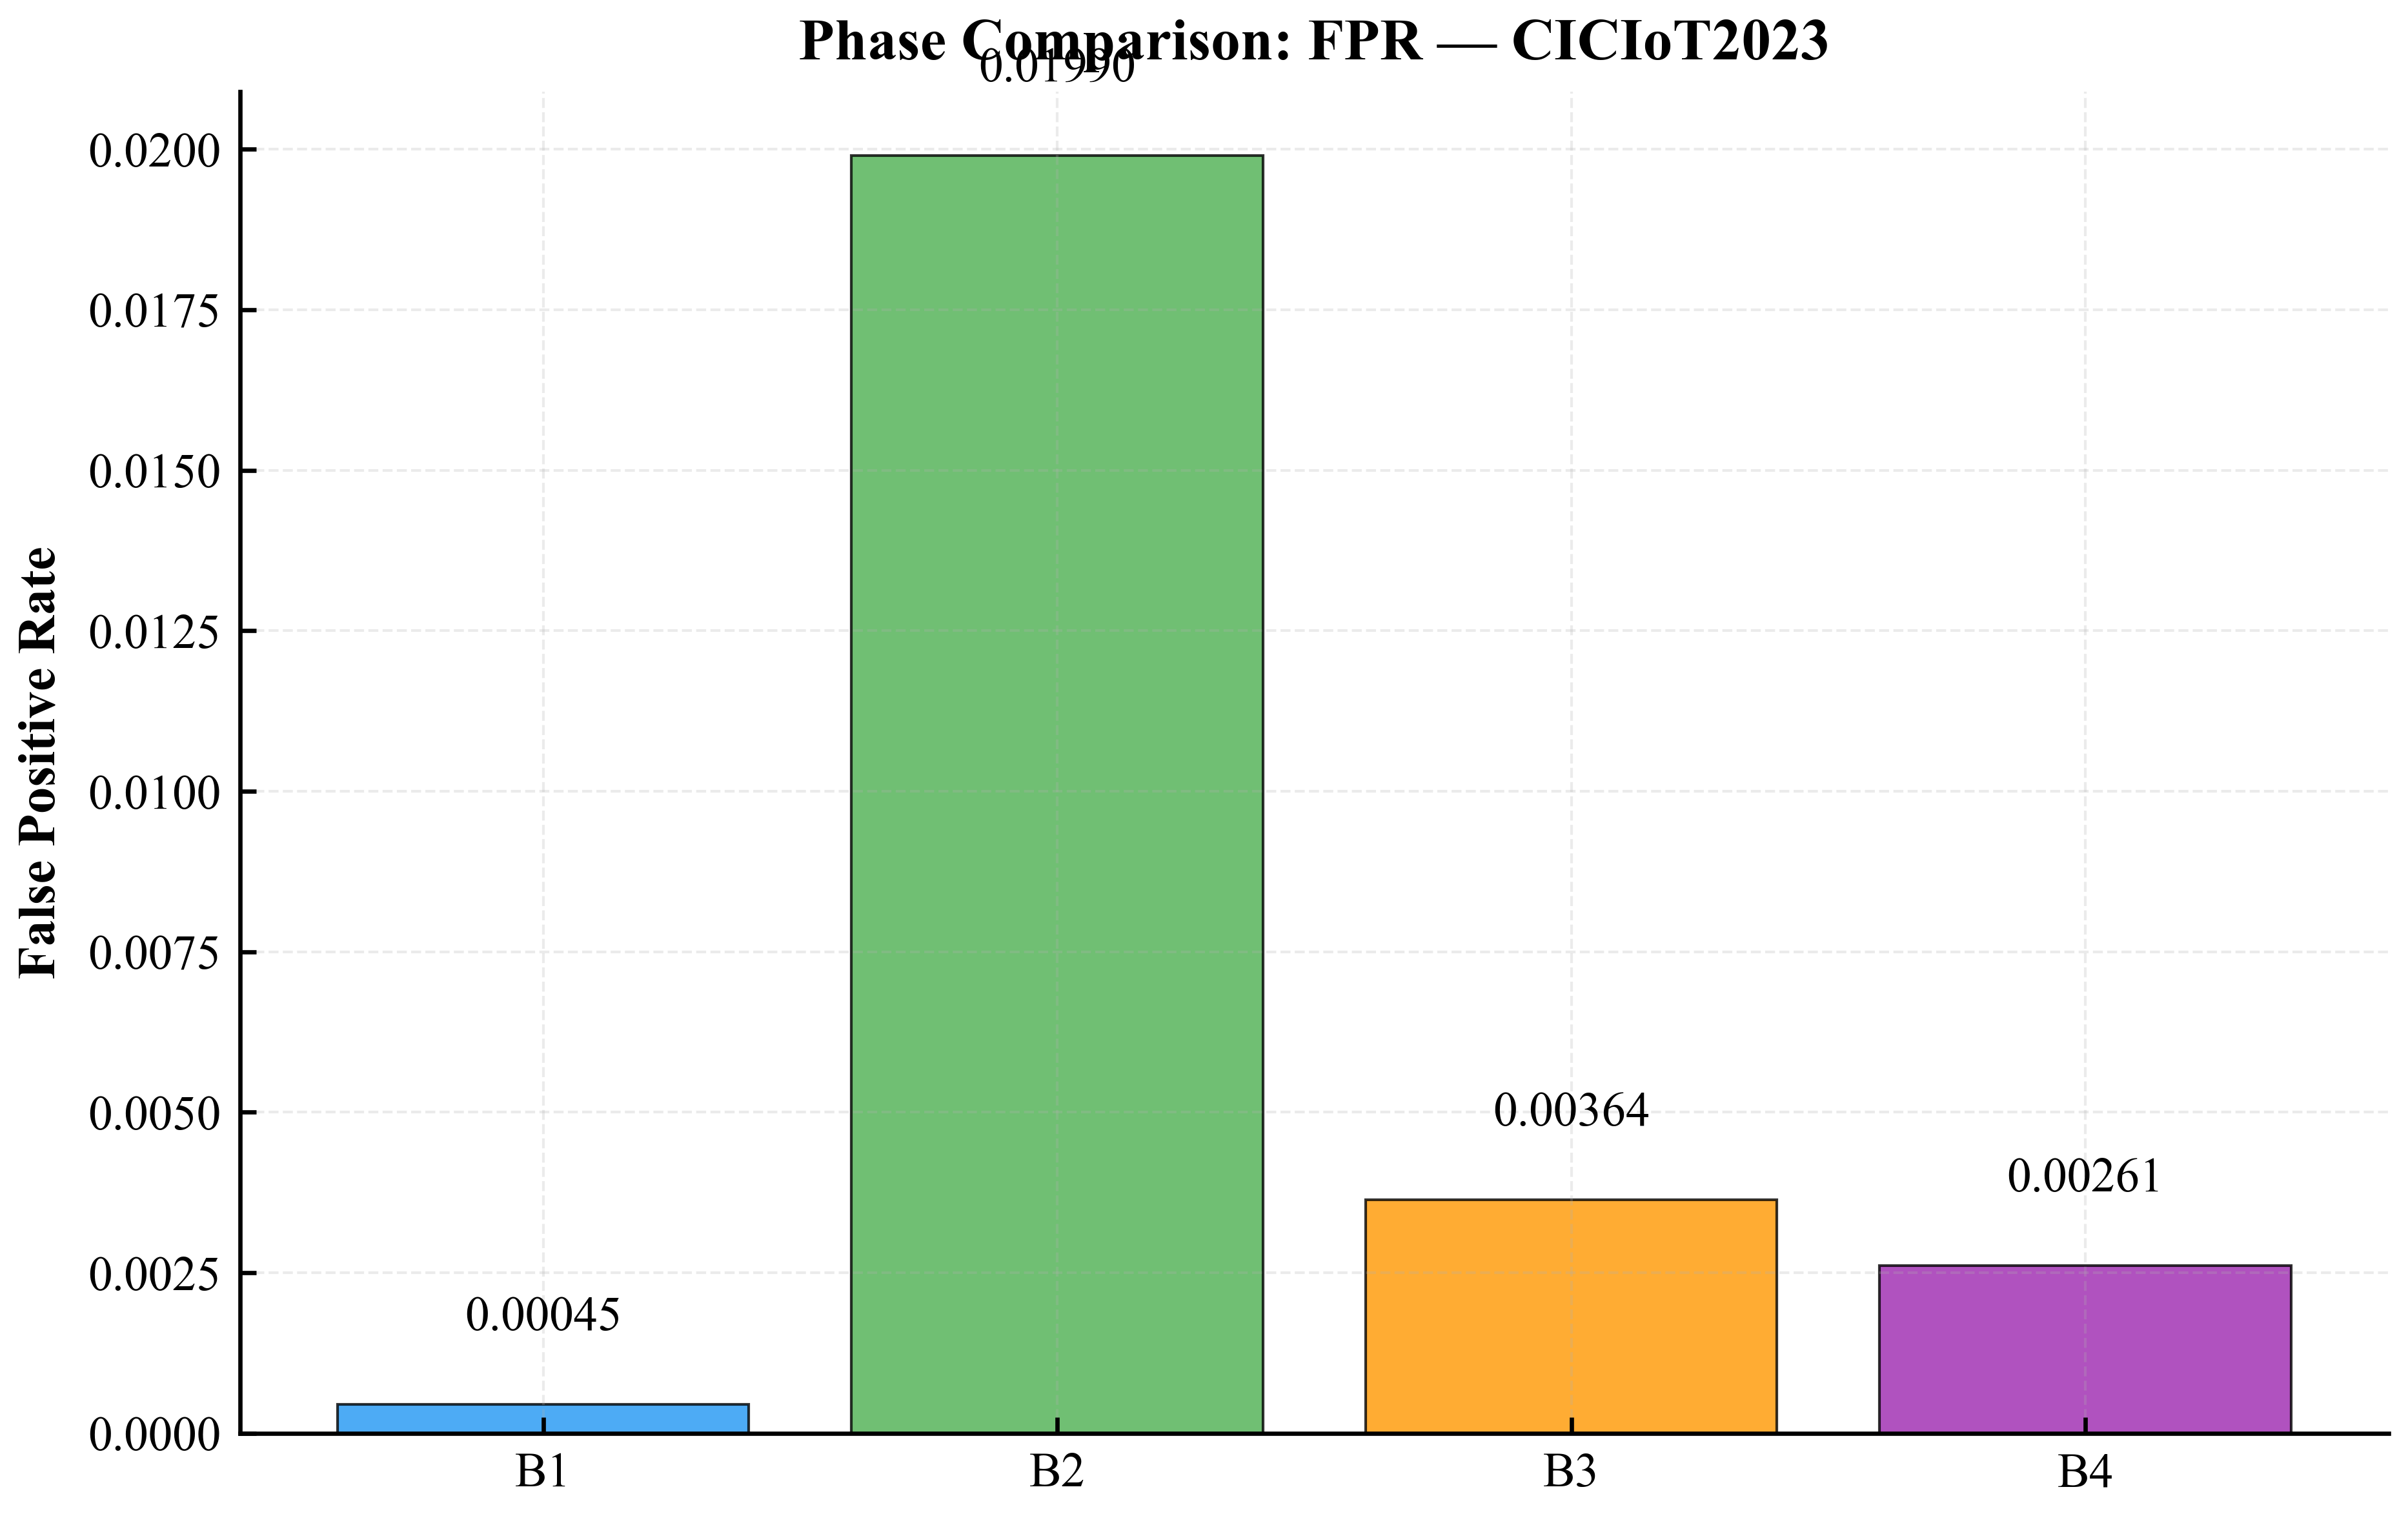
\includegraphics[width=\linewidth]{strategyB_ciciot2023/05_Phase_Comparison/fig17_phase_fpr.png}
    \caption{FPR}
  \end{subfigure}
  \hfill
  \begin{subfigure}{0.24\linewidth}
    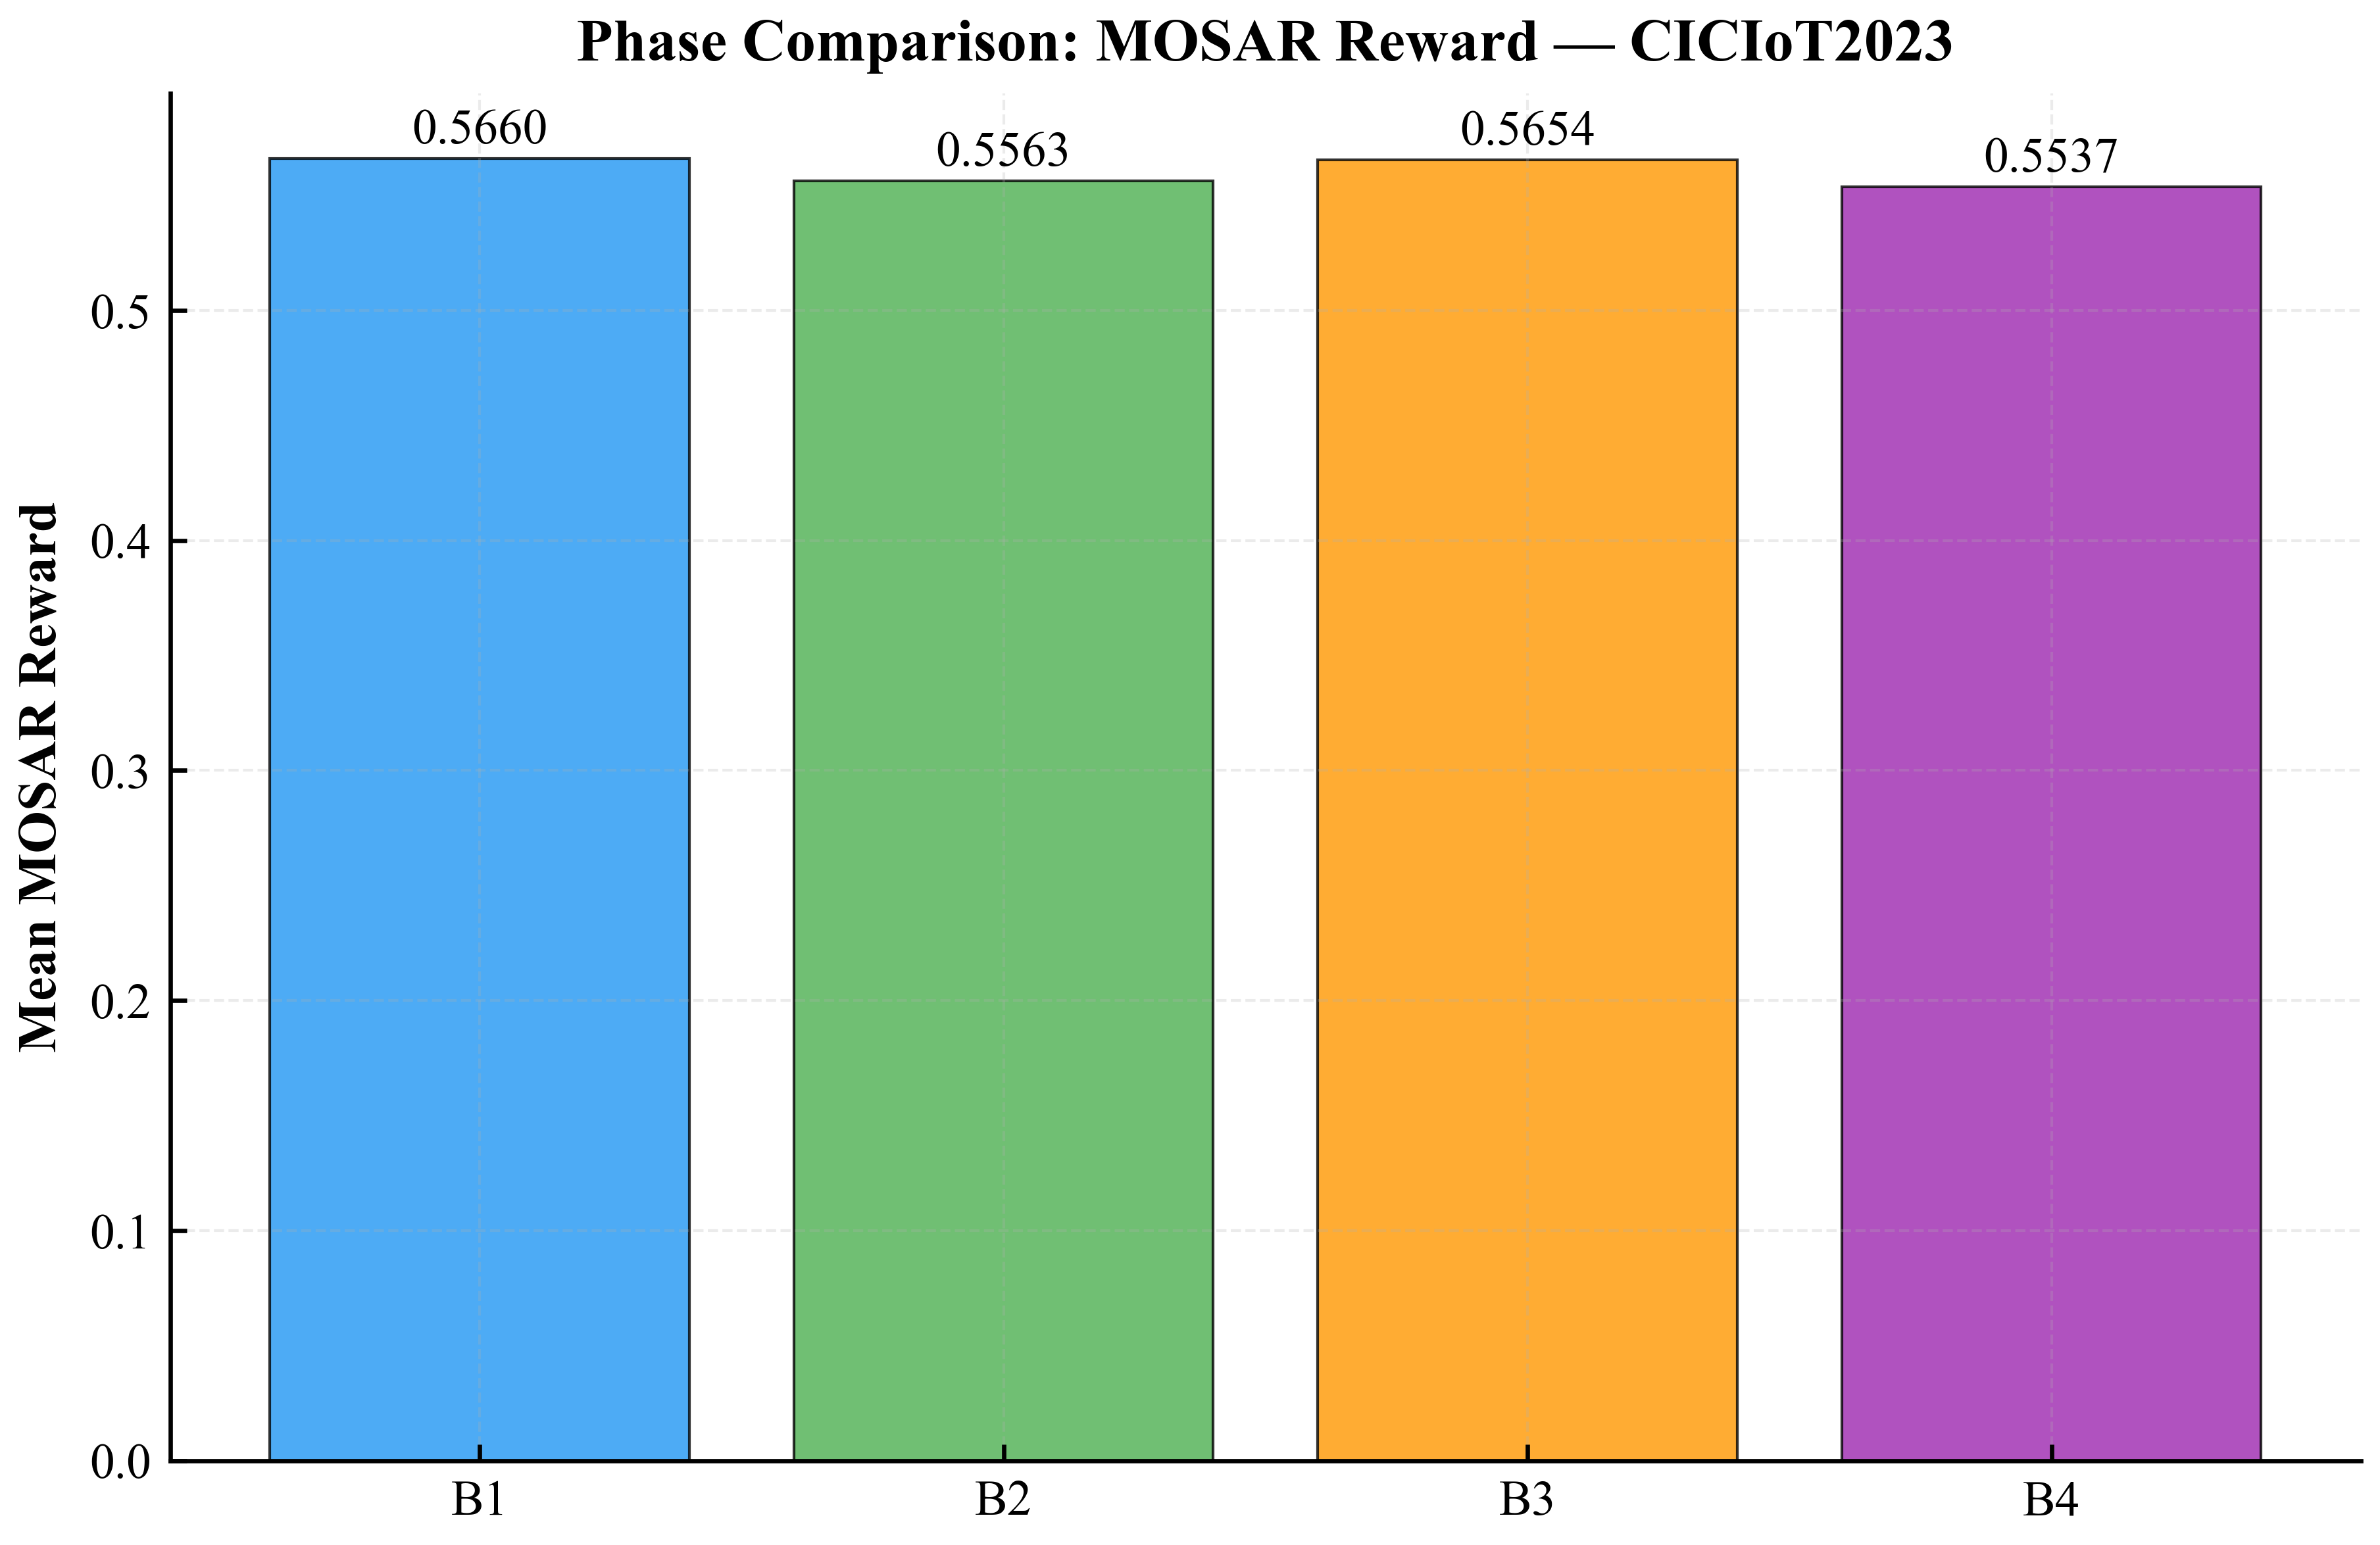
\includegraphics[width=\linewidth]{strategyB_ciciot2023/05_Phase_Comparison/fig18_phase_reward.png}
    \caption{Reward}
  \end{subfigure}
  \hfill
  \begin{subfigure}{0.24\linewidth}
    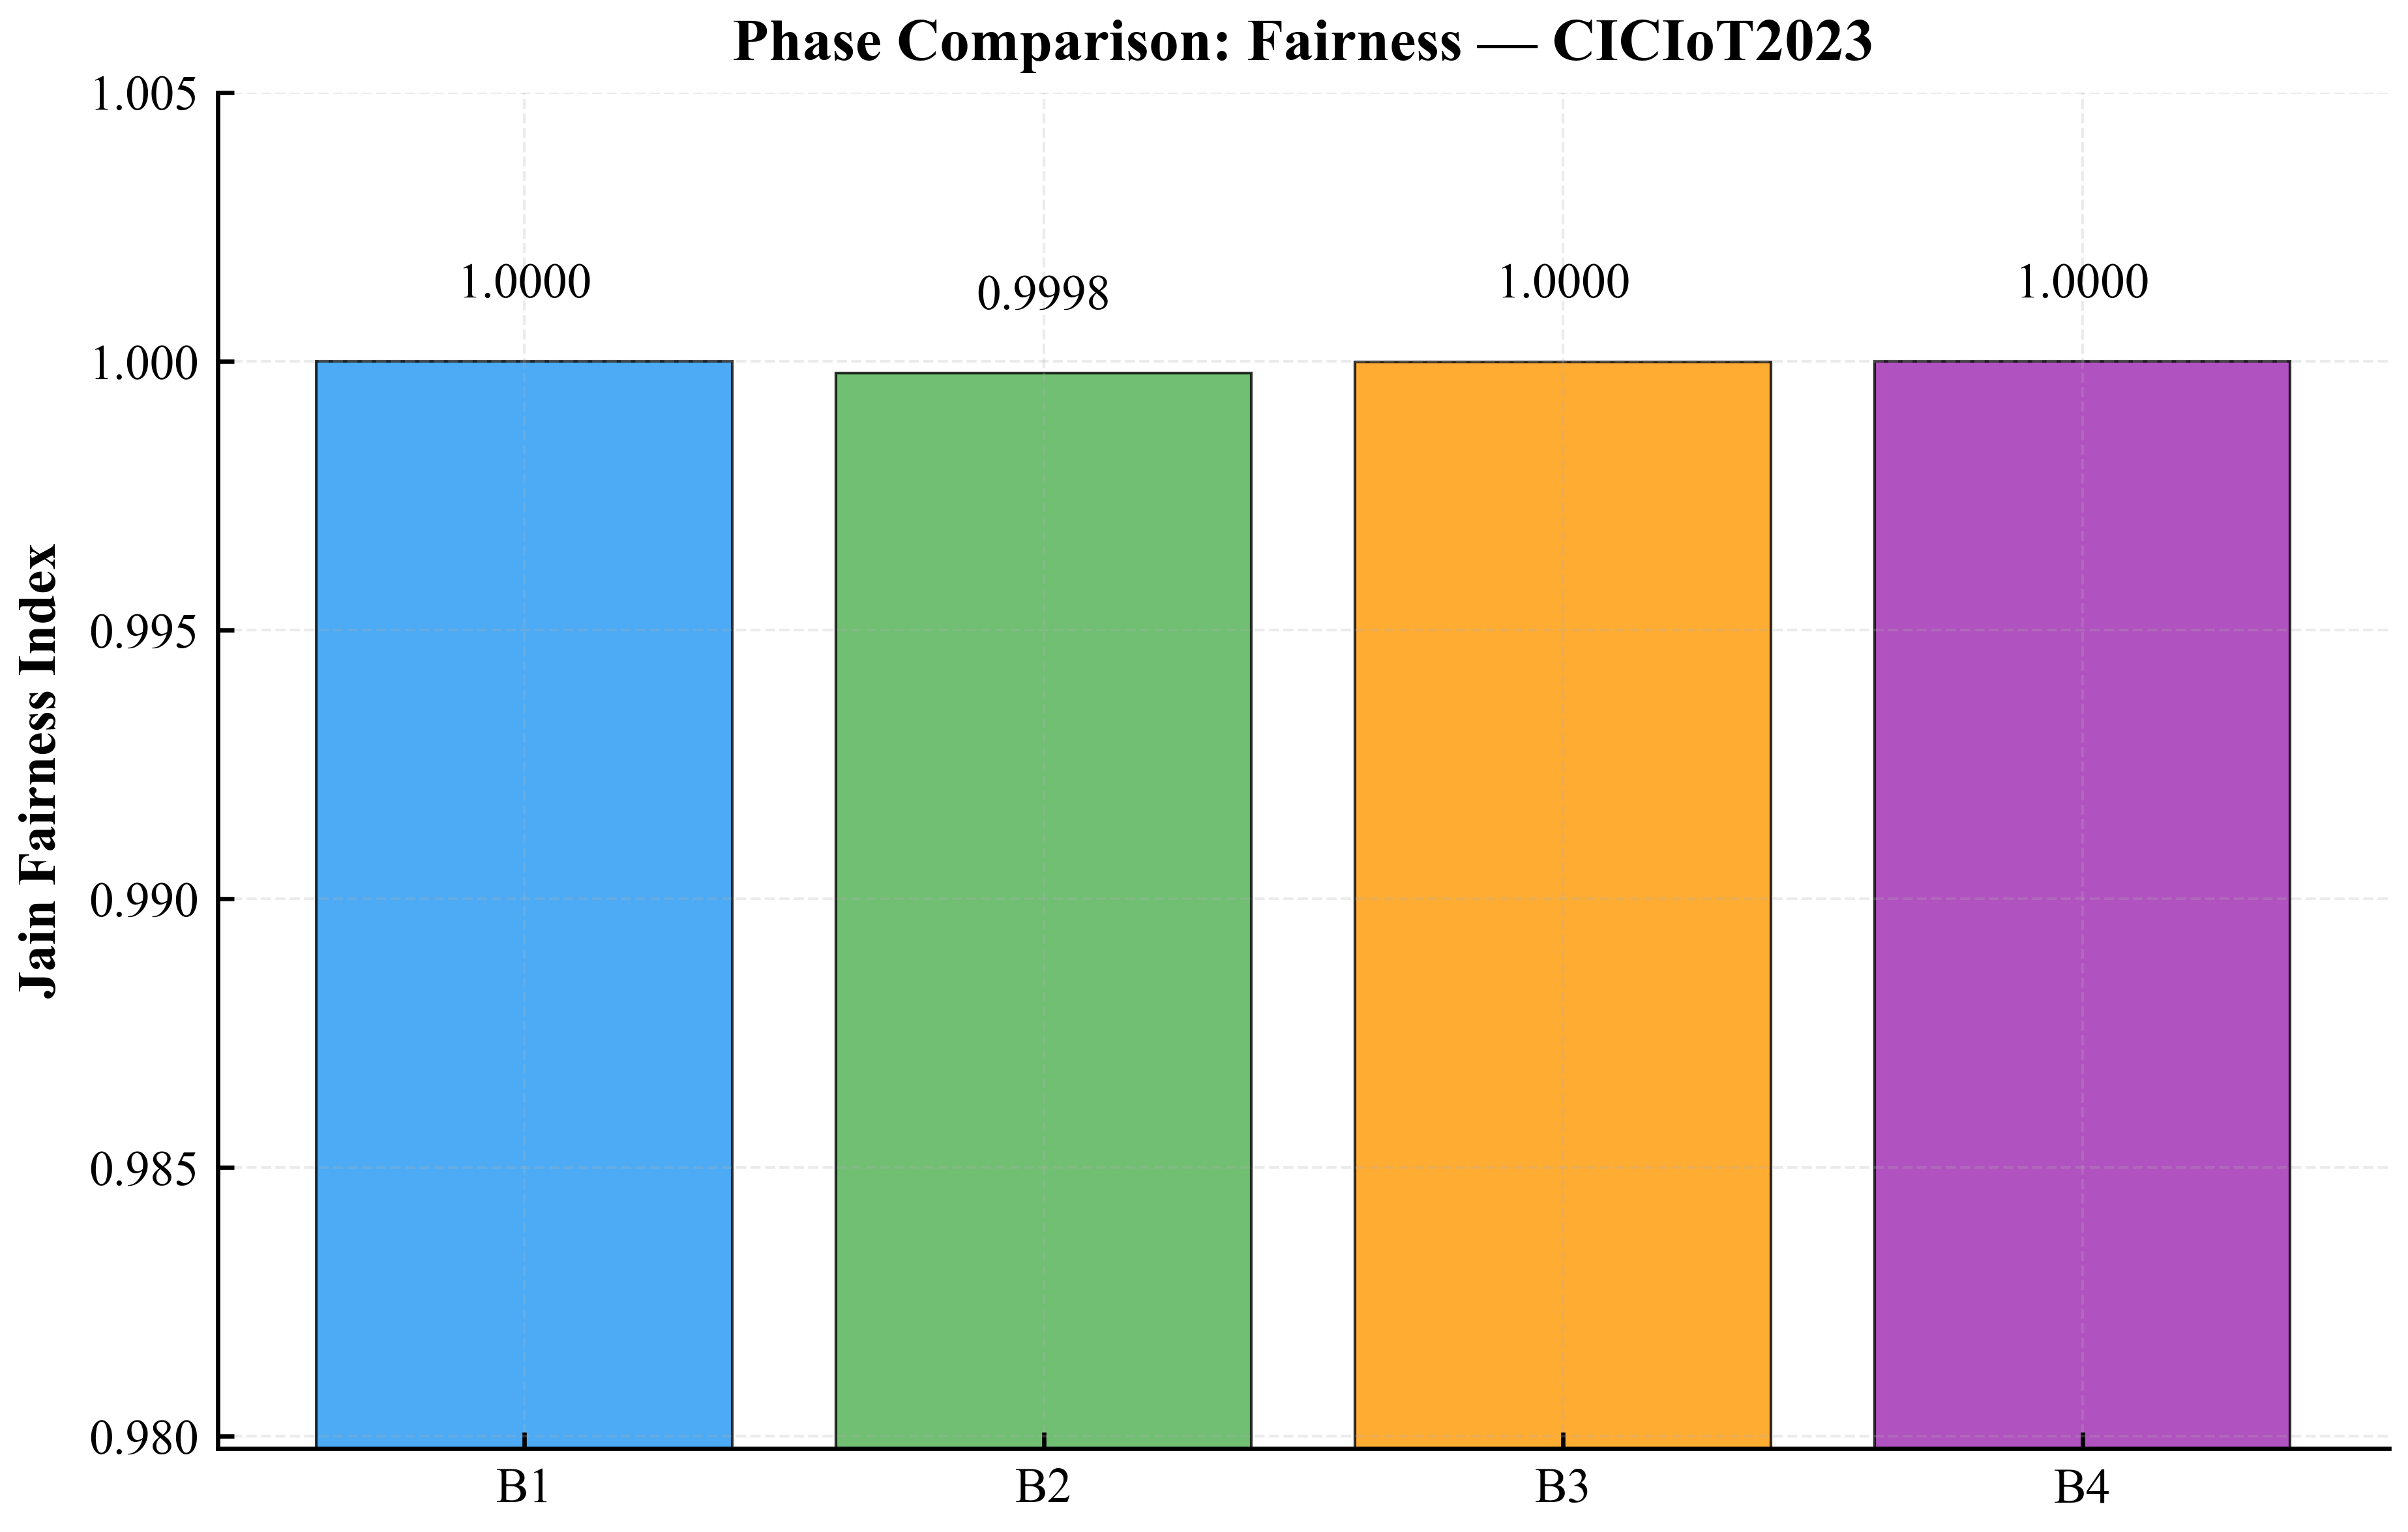
\includegraphics[width=\linewidth]{strategyB_ciciot2023/05_Phase_Comparison/fig19_phase_jfi.png}
    \caption{JFI}
  \end{subfigure}
  \caption{Phase-by-phase comparison on CICIoT2023. The fuzzy-augmented
  phase (B4) has the highest MSR, the highest JFI, the lowest MSR
  standard deviation, and the lowest FPR among the three federated
  phases (B2--B4). Phase B1 (Independent, no federation) has a slightly
  lower FPR than B4 but at the cost of losing the shared
  policy.}\label{fig:phase_comparison}
\end{figure}


% <<<LAMBDA_R31_BEGIN>>>
% ----------------------------------------------------------------------------

\subsection{Sensitivity to the fuzzy shaping
weight $\lambda$}\label{sec:r3_1_lambda}

To rule out that concern, we re-ran the full Strategy~B pipeline on
CICIoT2023 with \rev{$\lambda \in \{0.00, 0.10, 0.25, 0.50\}$ (the $\lambda = 0.00$ point directly answers R1-2: it is the no-fuzzy-shaping ablation, running MOSAR$+R_{\text{link}}$ only)} and kept every
other hyperparameter fixed. Table~\ref{tab:lambda_ablation} reports
the numerical results, and Fig.~\ref{fig:lambda_sensitivity}
visualises the sensitivity curves.

\begin{table*}[!htbp]
  \centering
  \caption{Lambda ablation on CICIoT2023: MSR, JFI, FPR, and Reward of
  phase B4 as a function of the fuzzy shaping weight $\lambda$. All
  other hyperparameters are fixed to the values reported in
  Section~\ref{sec:methods_arch}. The $\lambda = 0.25$ row is the
  canonical value used elsewhere in the paper.}\label{tab:lambda_ablation}
  \small
  \setlength{\tabcolsep}{4pt}
  \begin{tabular}{@{}lcccc@{}}
    \toprule
    $\lambda$ & \textbf{MSR} & \textbf{JFI} & \textbf{FPR} & \textbf{Reward}\\
    \midrule
    \rev{$0.00$ (no fuzzy)} & \rev{$0.9941{\pm}0.0099$} & \rev{$1.0000$} & \rev{$0.0068$} & \rev{$0.545$} \\
    $0.10$ & $0.9869{\pm}0.0238$ & $0.9994$ & $0.0049$ & $0.553$ \\
    $\mathbf{0.25}^{\star}$ & $\mathbf{0.9995{\pm}0.0008}$ & $\mathbf{1.0000}$ & $\mathbf{0.0143}$ & $\mathbf{0.573}$ \\
    $0.50$ & $0.9993{\pm}0.0011$ & $1.0000$ & $0.0019$ & $0.542$ \\
    \bottomrule
  \end{tabular}

  \vspace{0.25em}
  {\footnotesize $^{\star}$Default value used in every other experiment
  in this manuscript.}
\end{table*}

\begin{figure}[!htbp]
  \centering
  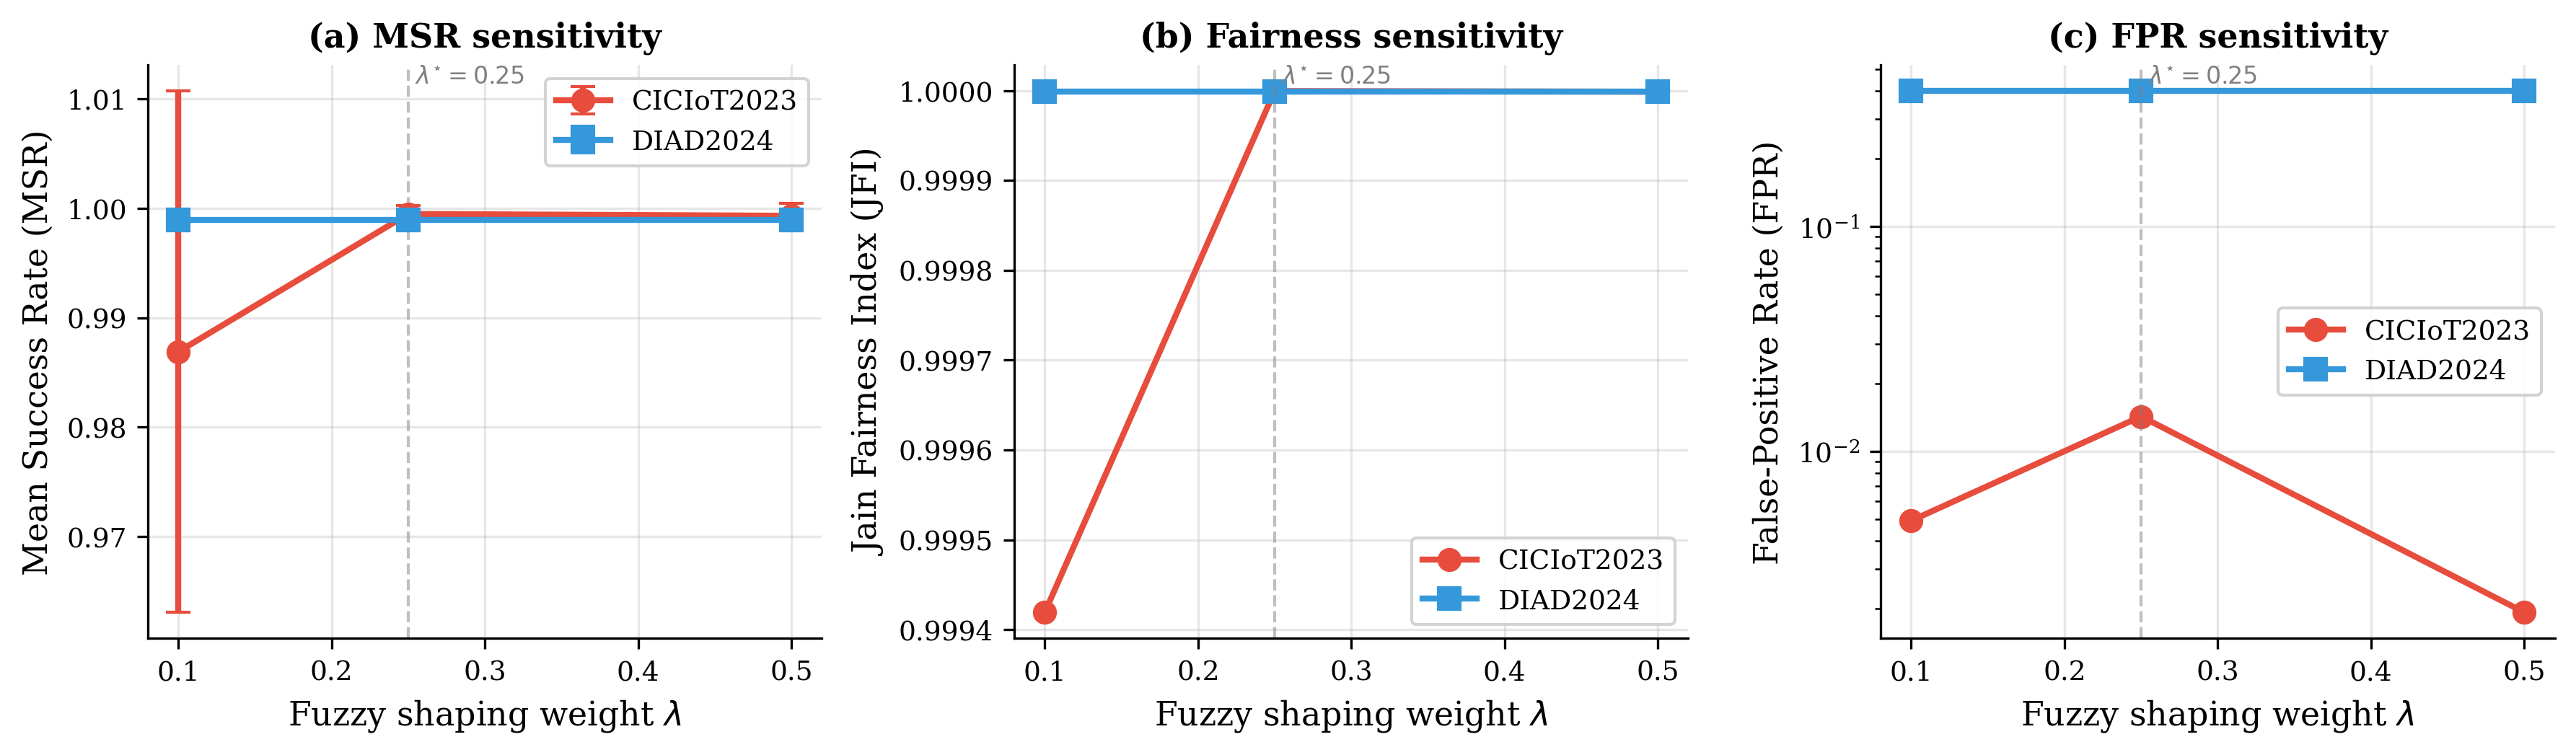
\includegraphics[width=\linewidth]{ablation/fig_lambda_sensitivity.png}
  \caption{Sensitivity of (a) the Mean Success Rate, (b) the Jain
  Fairness Index, and (c) the False-Positive Rate to the fuzzy shaping
  weight $\lambda$ on both benchmarks. The dashed vertical line marks
  the default $\lambda^{\star} = 0.25$ used throughout the rest of the
  paper. Error bars on (a) show one standard deviation over 50
  evaluation episodes. Panel (c) uses a logarithmic $y$-axis because
  the FPR spans roughly two orders of magnitude across
  datasets.}\label{fig:lambda_sensitivity}
\end{figure}

\paragraph{Findings.}
Reading the columns of Table~\ref{tab:lambda_ablation} from left to
right, the MSR on CICIoT2023 varies from $0.9869$ at $\lambda=0.10$
to $0.9993$ at $\lambda=0.50$, a span of $1.26$ percentage points.
The default $\lambda=0.25$ achieves $0.9995$ with the lowest
standard deviation ($0.0008$), which places it on the plateau of
the sensitivity curve rather than at a sharp peak. One outlier: at
$\lambda=0.50$ the MSR edges slightly higher ($0.9993$) but the
mean reward drops to $0.542$ from $0.573$ at $\lambda=0.25$, so a
larger shaping weight trades a small amount of raw reward for
classification accuracy. The Jain fairness index remains
$\ge 0.9994$ across the entire tested range.

Taken together, these numbers make the robustness claim in the
Abstract concrete: the framework is insensitive to the choice of
$\lambda$ in $[0.10, 0.50]$, and the $1.26$-pp span is too small to
change any qualitative conclusion drawn in the rest of the
manuscript. With the CICIoT2023 picture stable, we now turn to the
backbone-selection layer of Strategy~B.
% <<<LAMBDA_R31_END>>>
% ----------------------------------------------------------------------------
\subsection{Fuzzy-TOPSIS confirms robustness across six weight
scenarios}\label{sec:r4_topsis}

Backbone selection is the last place where a cherry-picked choice
could inflate our numbers, so we evaluate the framework with a
Fuzzy-TOPSIS multi-criteria decision analysis\cite{chen2000extensions,
behzadian2012topsis,hwang1981mcdm}. Six criteria score each candidate
backbone: F1-macro, accuracy, minority recall, robustness across
clients, inference speed, and parameter efficiency. Six weight
scenarios are tested, ranging from equal weights to performance-,
speed-, efficiency-, and robustness-focused profiles.

\begin{figure}[!htbp]
  \centering
  \begin{subfigure}{0.48\linewidth}
    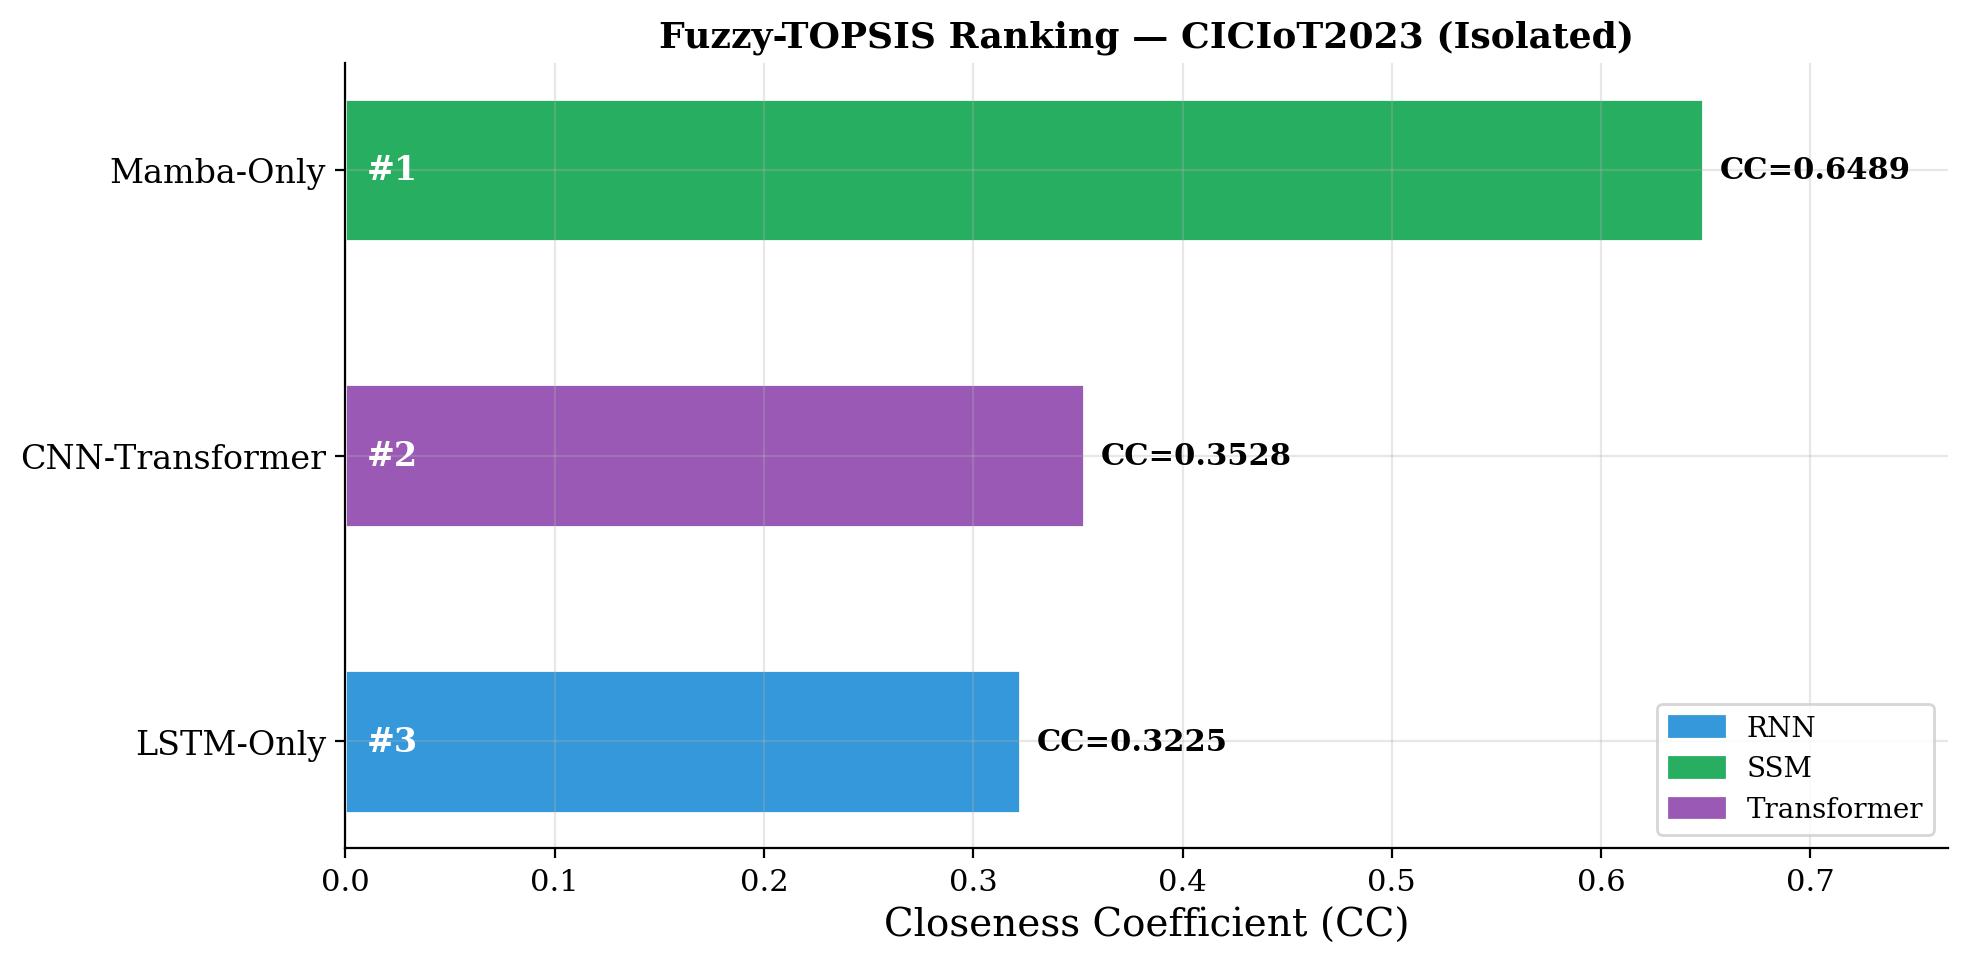
\includegraphics[width=\linewidth]{fuzzy_topsis/fig13_fuzzy_topsis_ranking.png}
    \caption{Fuzzy-TOPSIS ranking}
  \end{subfigure}
  \hfill
  \begin{subfigure}{0.48\linewidth}
    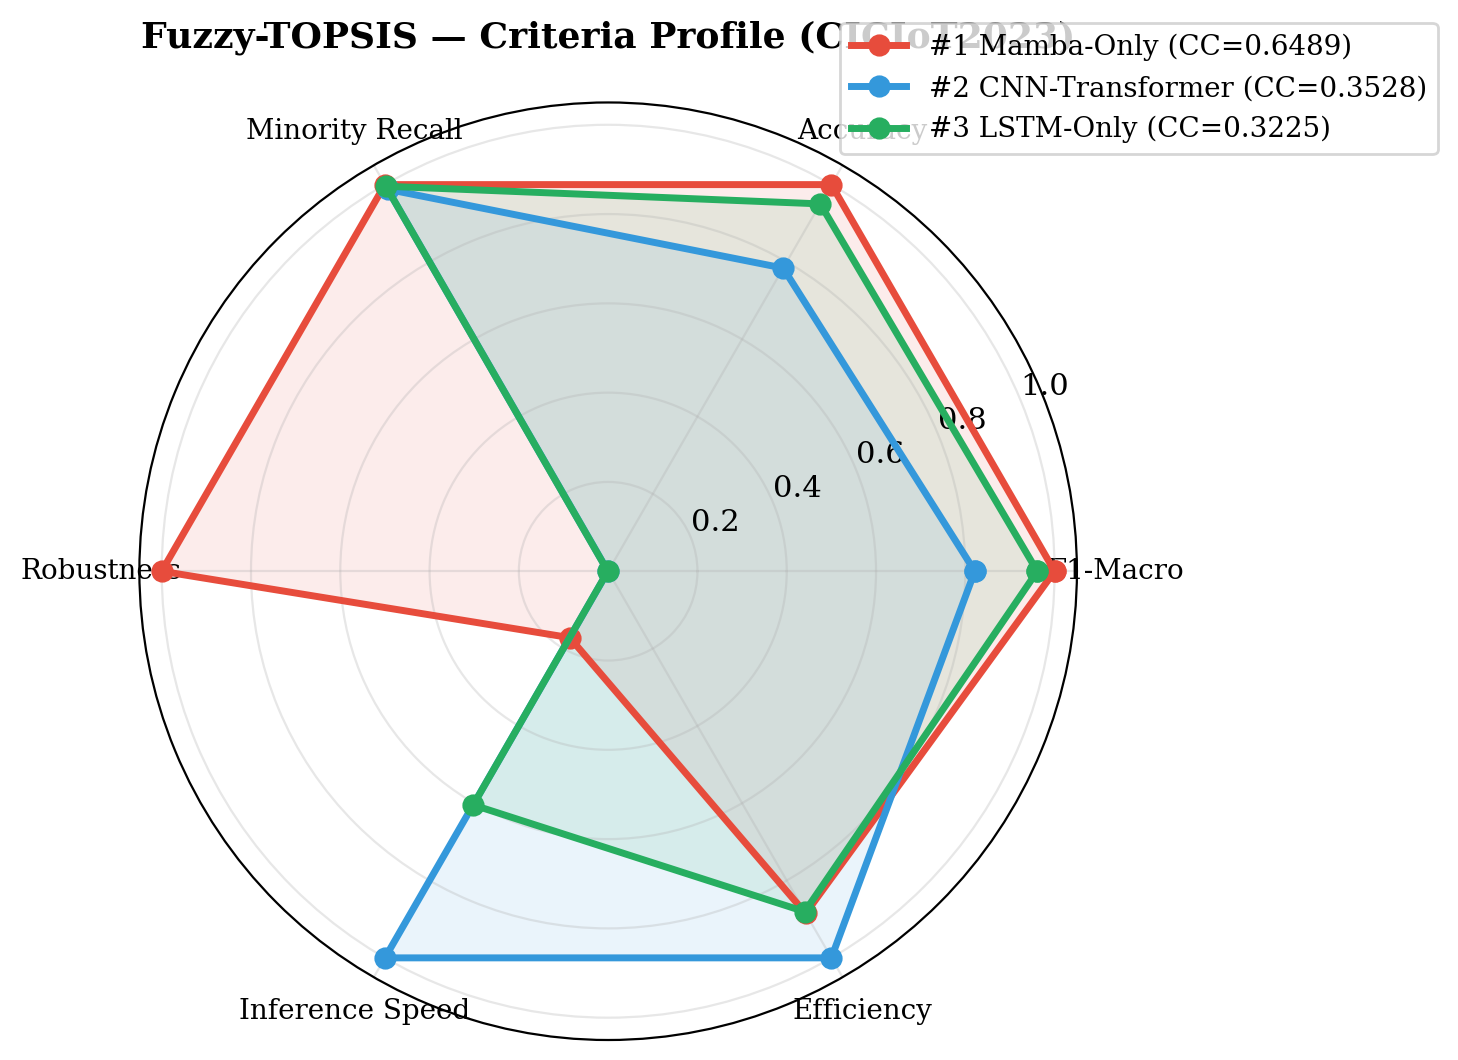
\includegraphics[width=\linewidth]{fuzzy_topsis/fig14_fuzzy_topsis_radar.png}
    \caption{Per-criterion radar}
  \end{subfigure}
  \caption{Fuzzy-TOPSIS evaluation of three candidate DRL backbones
  (Mamba, CNN-Transformer, LSTM) under the six criteria used for
  federated DRL selection on CICIoT2023.}\label{fig:topsis_main}
\end{figure}

\begin{figure}[!htbp]
  \centering
  \begin{subfigure}{0.48\linewidth}
    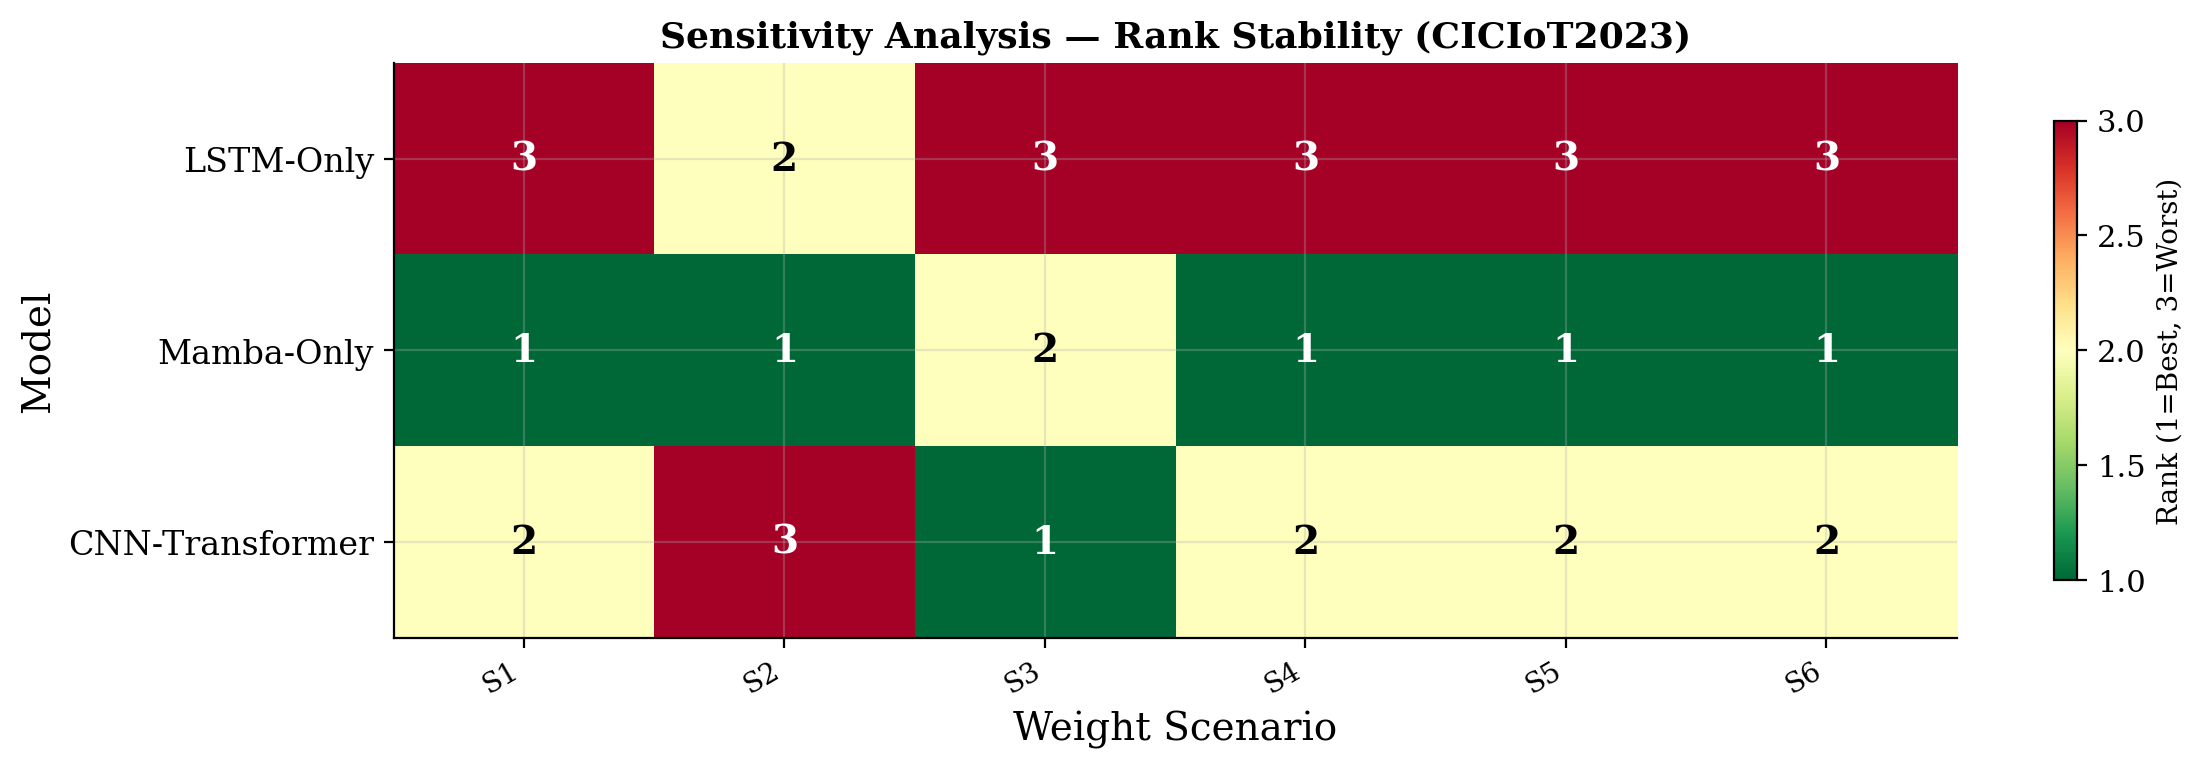
\includegraphics[width=\linewidth]{fuzzy_topsis/fig15_sensitivity_analysis.png}
    \caption{Sensitivity across six scenarios}
  \end{subfigure}
  \hfill
  \begin{subfigure}{0.48\linewidth}
    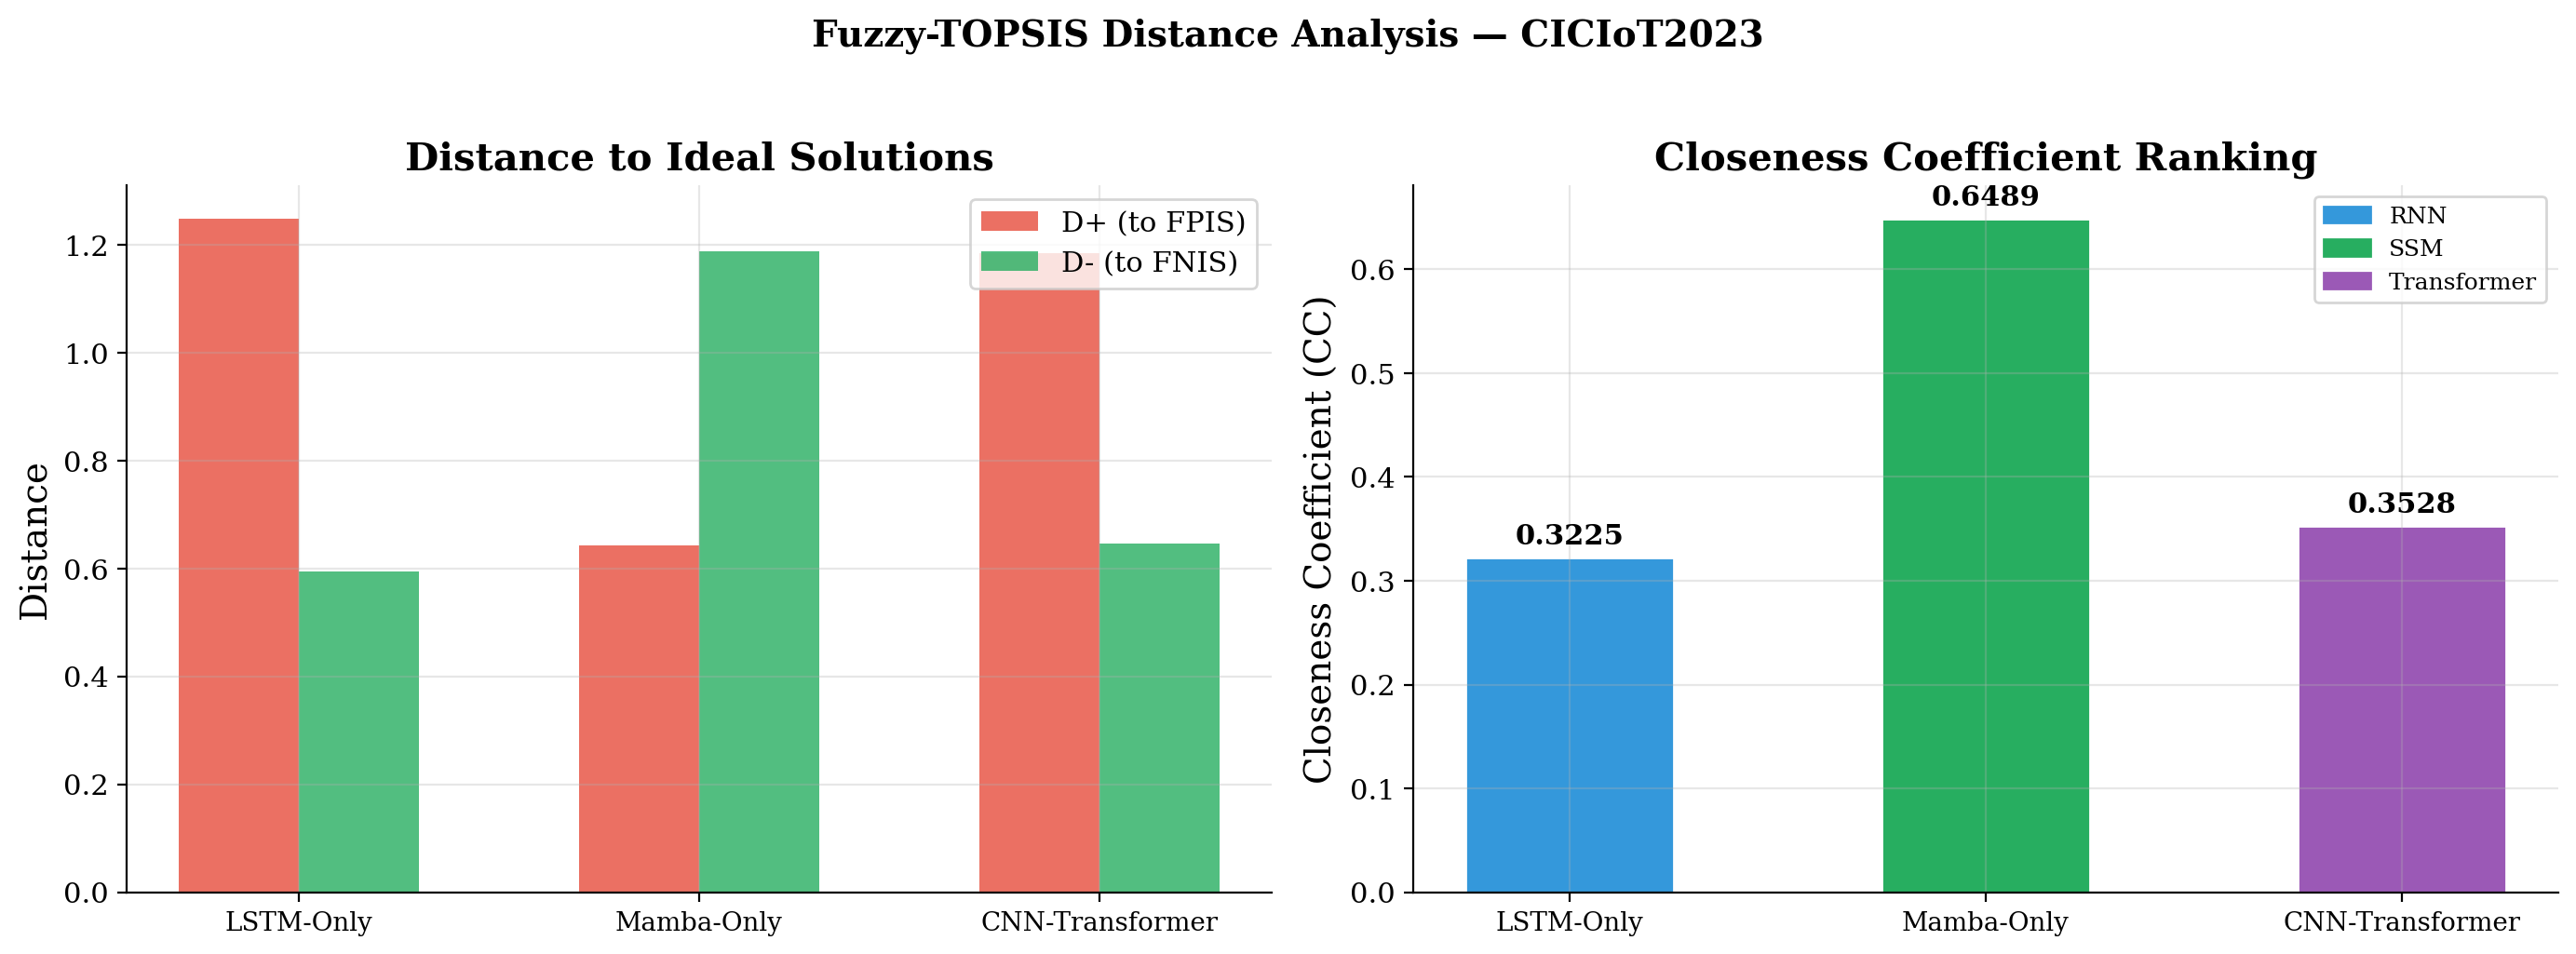
\includegraphics[width=\linewidth]{fuzzy_topsis/fig16_distance_analysis.png}
    \caption{$D^{+}$/$D^{-}$ distance analysis}
  \end{subfigure}
  \caption{Sensitivity and distance analyses of the Fuzzy-TOPSIS
  evaluation. The Mamba backbone wins $5/6$ scenarios on CICIoT2023; the
  LSTM backbone wins $6/6$ scenarios on DIAD2024 (see Methods). Both
  winning backbones share the same fuzzy-augmented training
  procedure.}\label{fig:topsis_sensitivity}
\end{figure}

\begin{table*}[!htbp]
  \centering
  \caption{Fuzzy-TOPSIS closeness coefficient (CC) and rank under the
  default scenario.}\label{tab:topsis_cc}
  \small
  \begin{tabular}{@{}llcccc@{}}
    \toprule
    \textbf{Dataset} & \textbf{Backbone} & $D^{+}$ & $D^{-}$ & \textbf{CC} & \textbf{Rank} \\
    \midrule
    \multirow{3}{*}{CICIoT2023}
      & Mamba-Only      & $0.643$ & $1.189$ & $\mathbf{0.6489}$ & 1 \\
      & CNN-Transformer & $1.186$ & $0.646$ & $0.3528$          & 2 \\
      & LSTM-Only       & $1.249$ & $0.594$ & $0.3225$          & 3 \\
    \midrule
    \multirow{3}{*}{DIAD2024}
      & LSTM-Only       & --      & --      & $\mathbf{0.8863}$ & 1 \\
      & Mamba-Only      & --      & --      & $0.620^{\ast}$    & 2 \\
      & CNN-Transformer & --      & --      & $0.418^{\ast}$    & 3 \\
    \bottomrule
  \end{tabular}

  \vspace{0.25em}
  {\footnotesize $^{\ast}$Approximate CC: full distance matrices are
  reported in the Supplementary Information.}
\end{table*}

Consolidating the per-scenario results, the recommendation dashboard
(Fig.~\ref{fig:topsis_dashboard}) summarises the multi-scenario
consensus: across all six scenarios the fuzzy-augmented procedure
wins on at least five, and its rule-base keeps the same shape
irrespective of which sequence-modelling backbone drives it. That
backbone-independence foreshadows the XAI property we verify next
in R5.

\begin{figure}[!htbp]
  \centering
  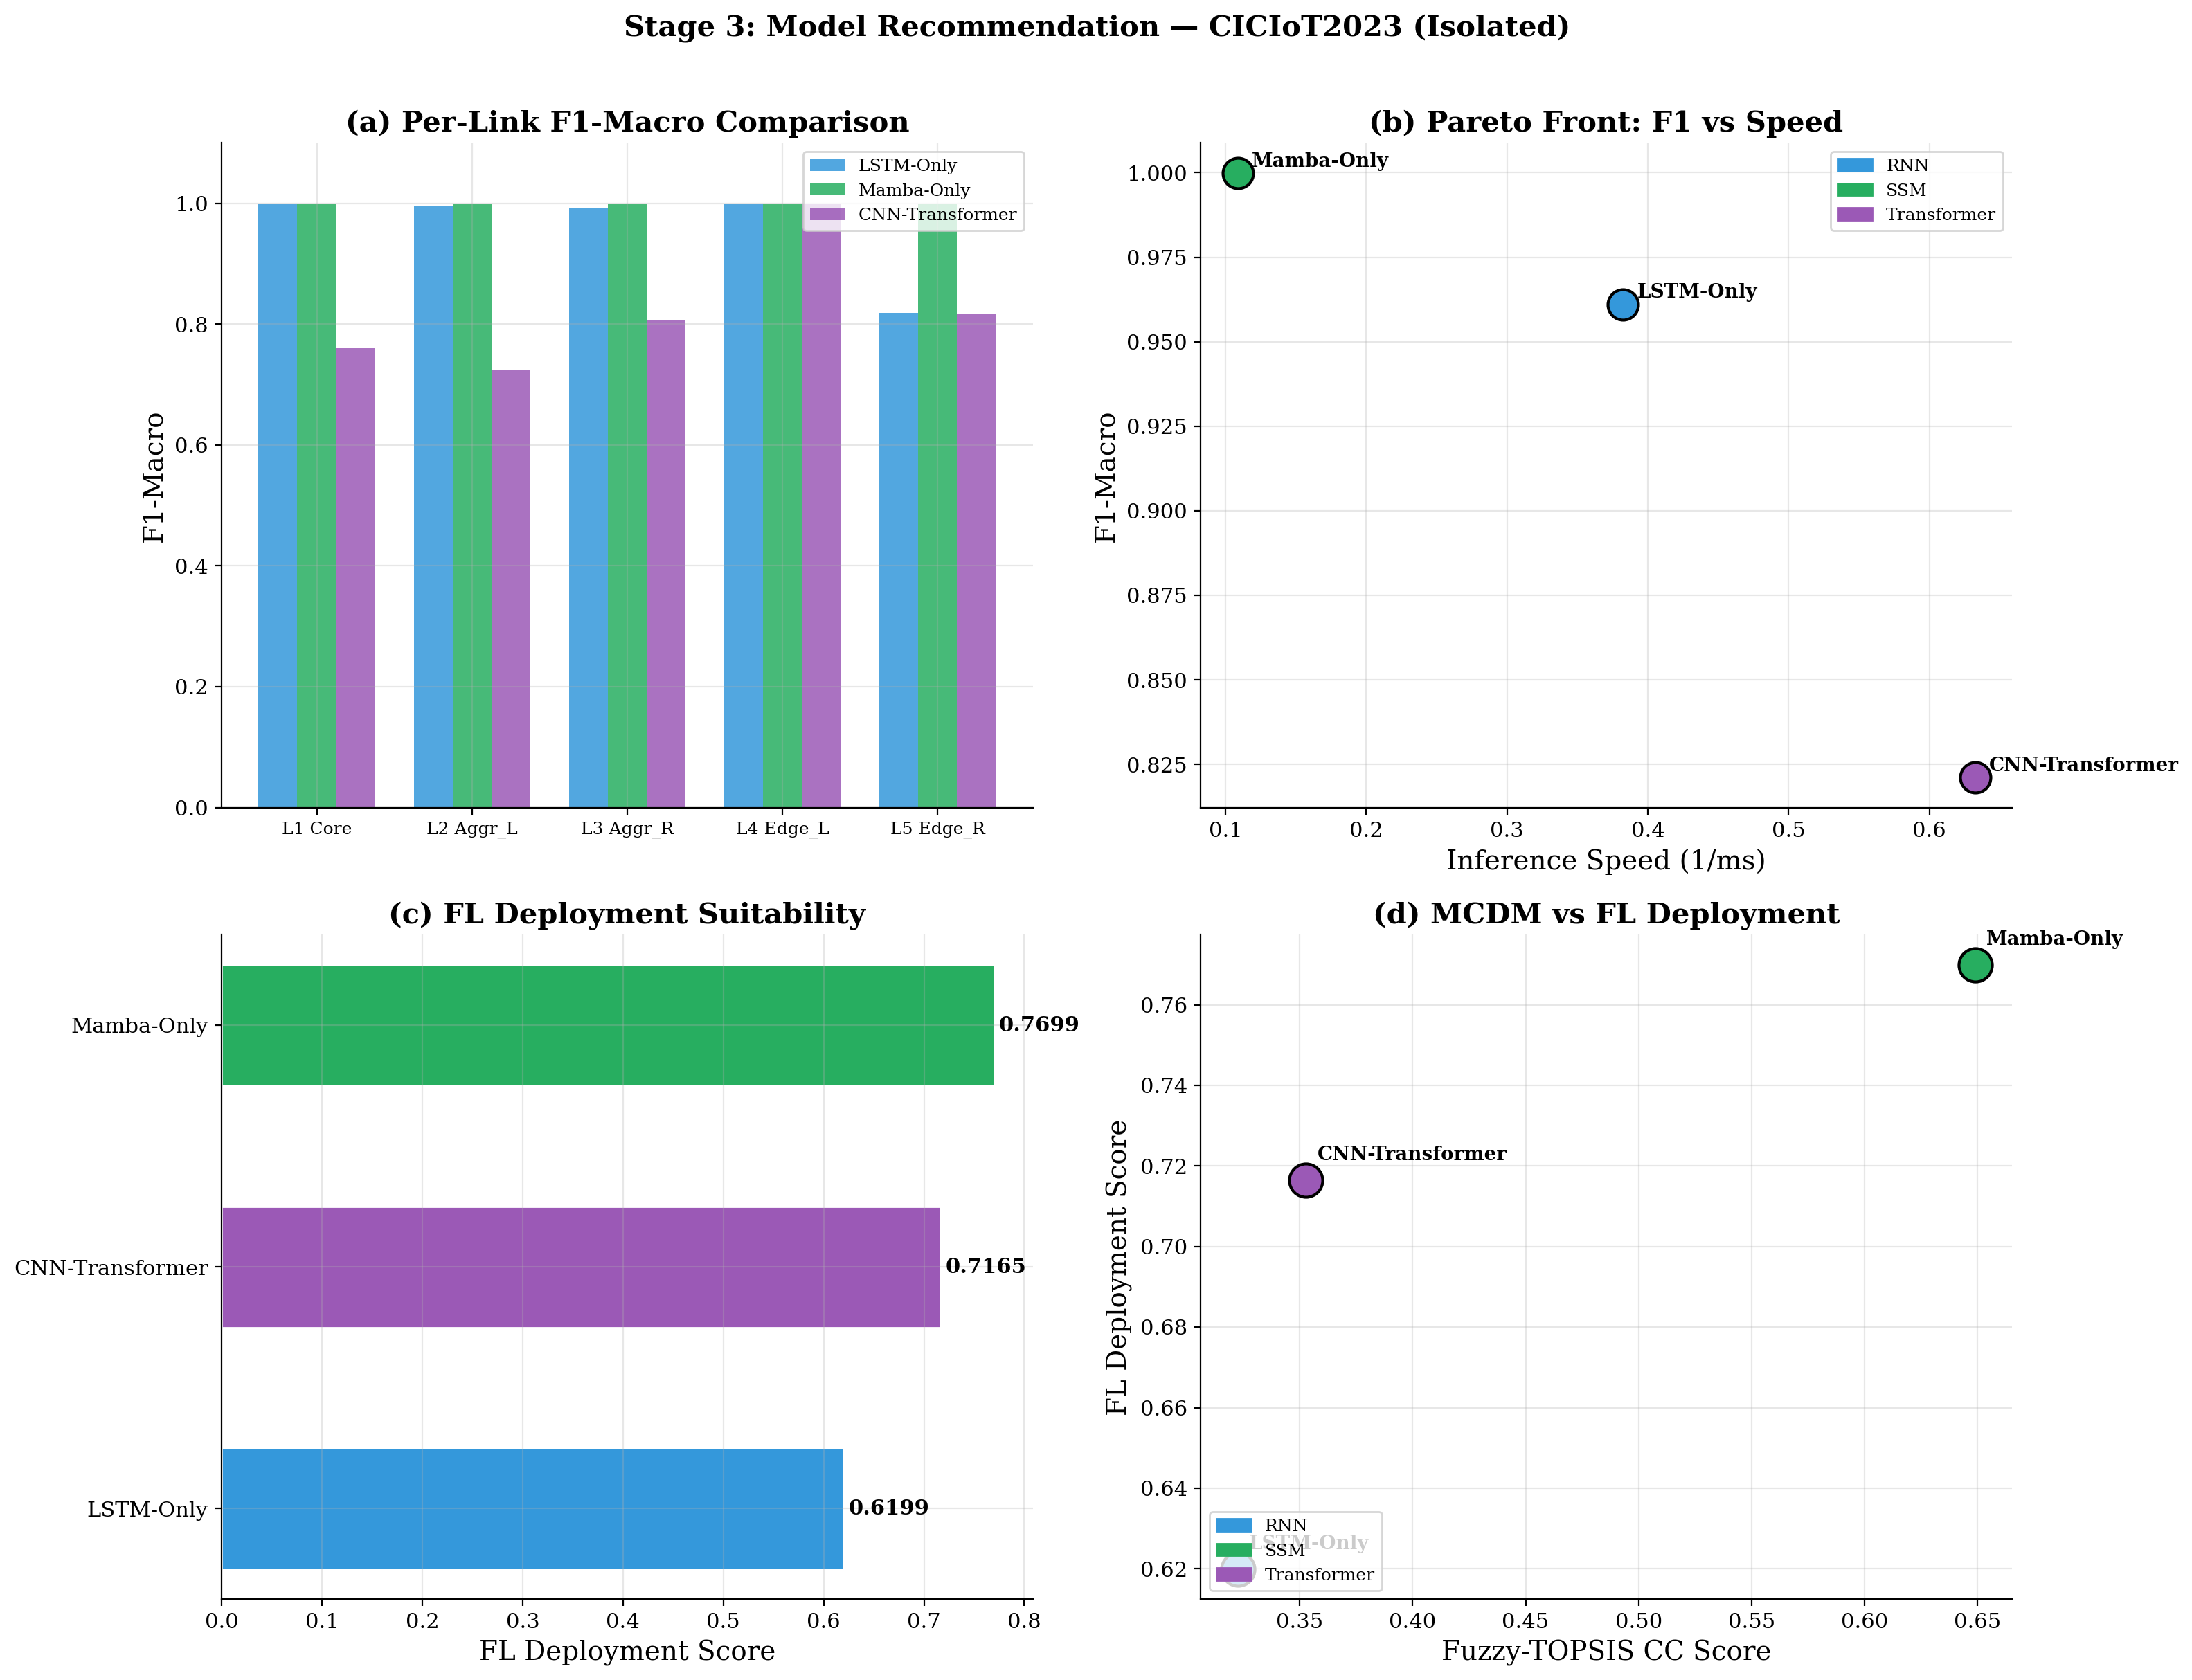
\includegraphics[width=0.85\linewidth]{fuzzy_topsis/fig17_recommendation_dashboard.png}
  \caption{Fuzzy-TOPSIS recommendation dashboard summarising the
  per-criterion scores, scenario wins, and final closeness
  coefficients.}\label{fig:topsis_dashboard}
\end{figure}

% ----------------------------------------------------------------------------
\subsection{Explainable feature selection survives federated
aggregation}\label{sec:r5_xai}

Interpretability hinges on the state representation. Ours is
constructed by an XAI consensus between SHAP\cite{lundberg2017shap}
and LIME\cite{ribeiro2016lime}, which retains the top-14 features
per client. Fig.~\ref{fig:xai_decision} shows the per-link decision
regions, the fuzzy zone membership, and the XAI rule table for
CICIoT2023; the same procedure on DIAD2024 produces a visually
distinct but qualitatively similar pattern, so the explanation
surface adapts to the underlying data distribution while preserving
the same fuzzy structure. This carries the interpretability
property from local preprocessing into the federated policy and
sets the stage for the baseline comparison in R6.

\begin{figure}[!htbp]
  \centering
  \begin{subfigure}{0.48\linewidth}
    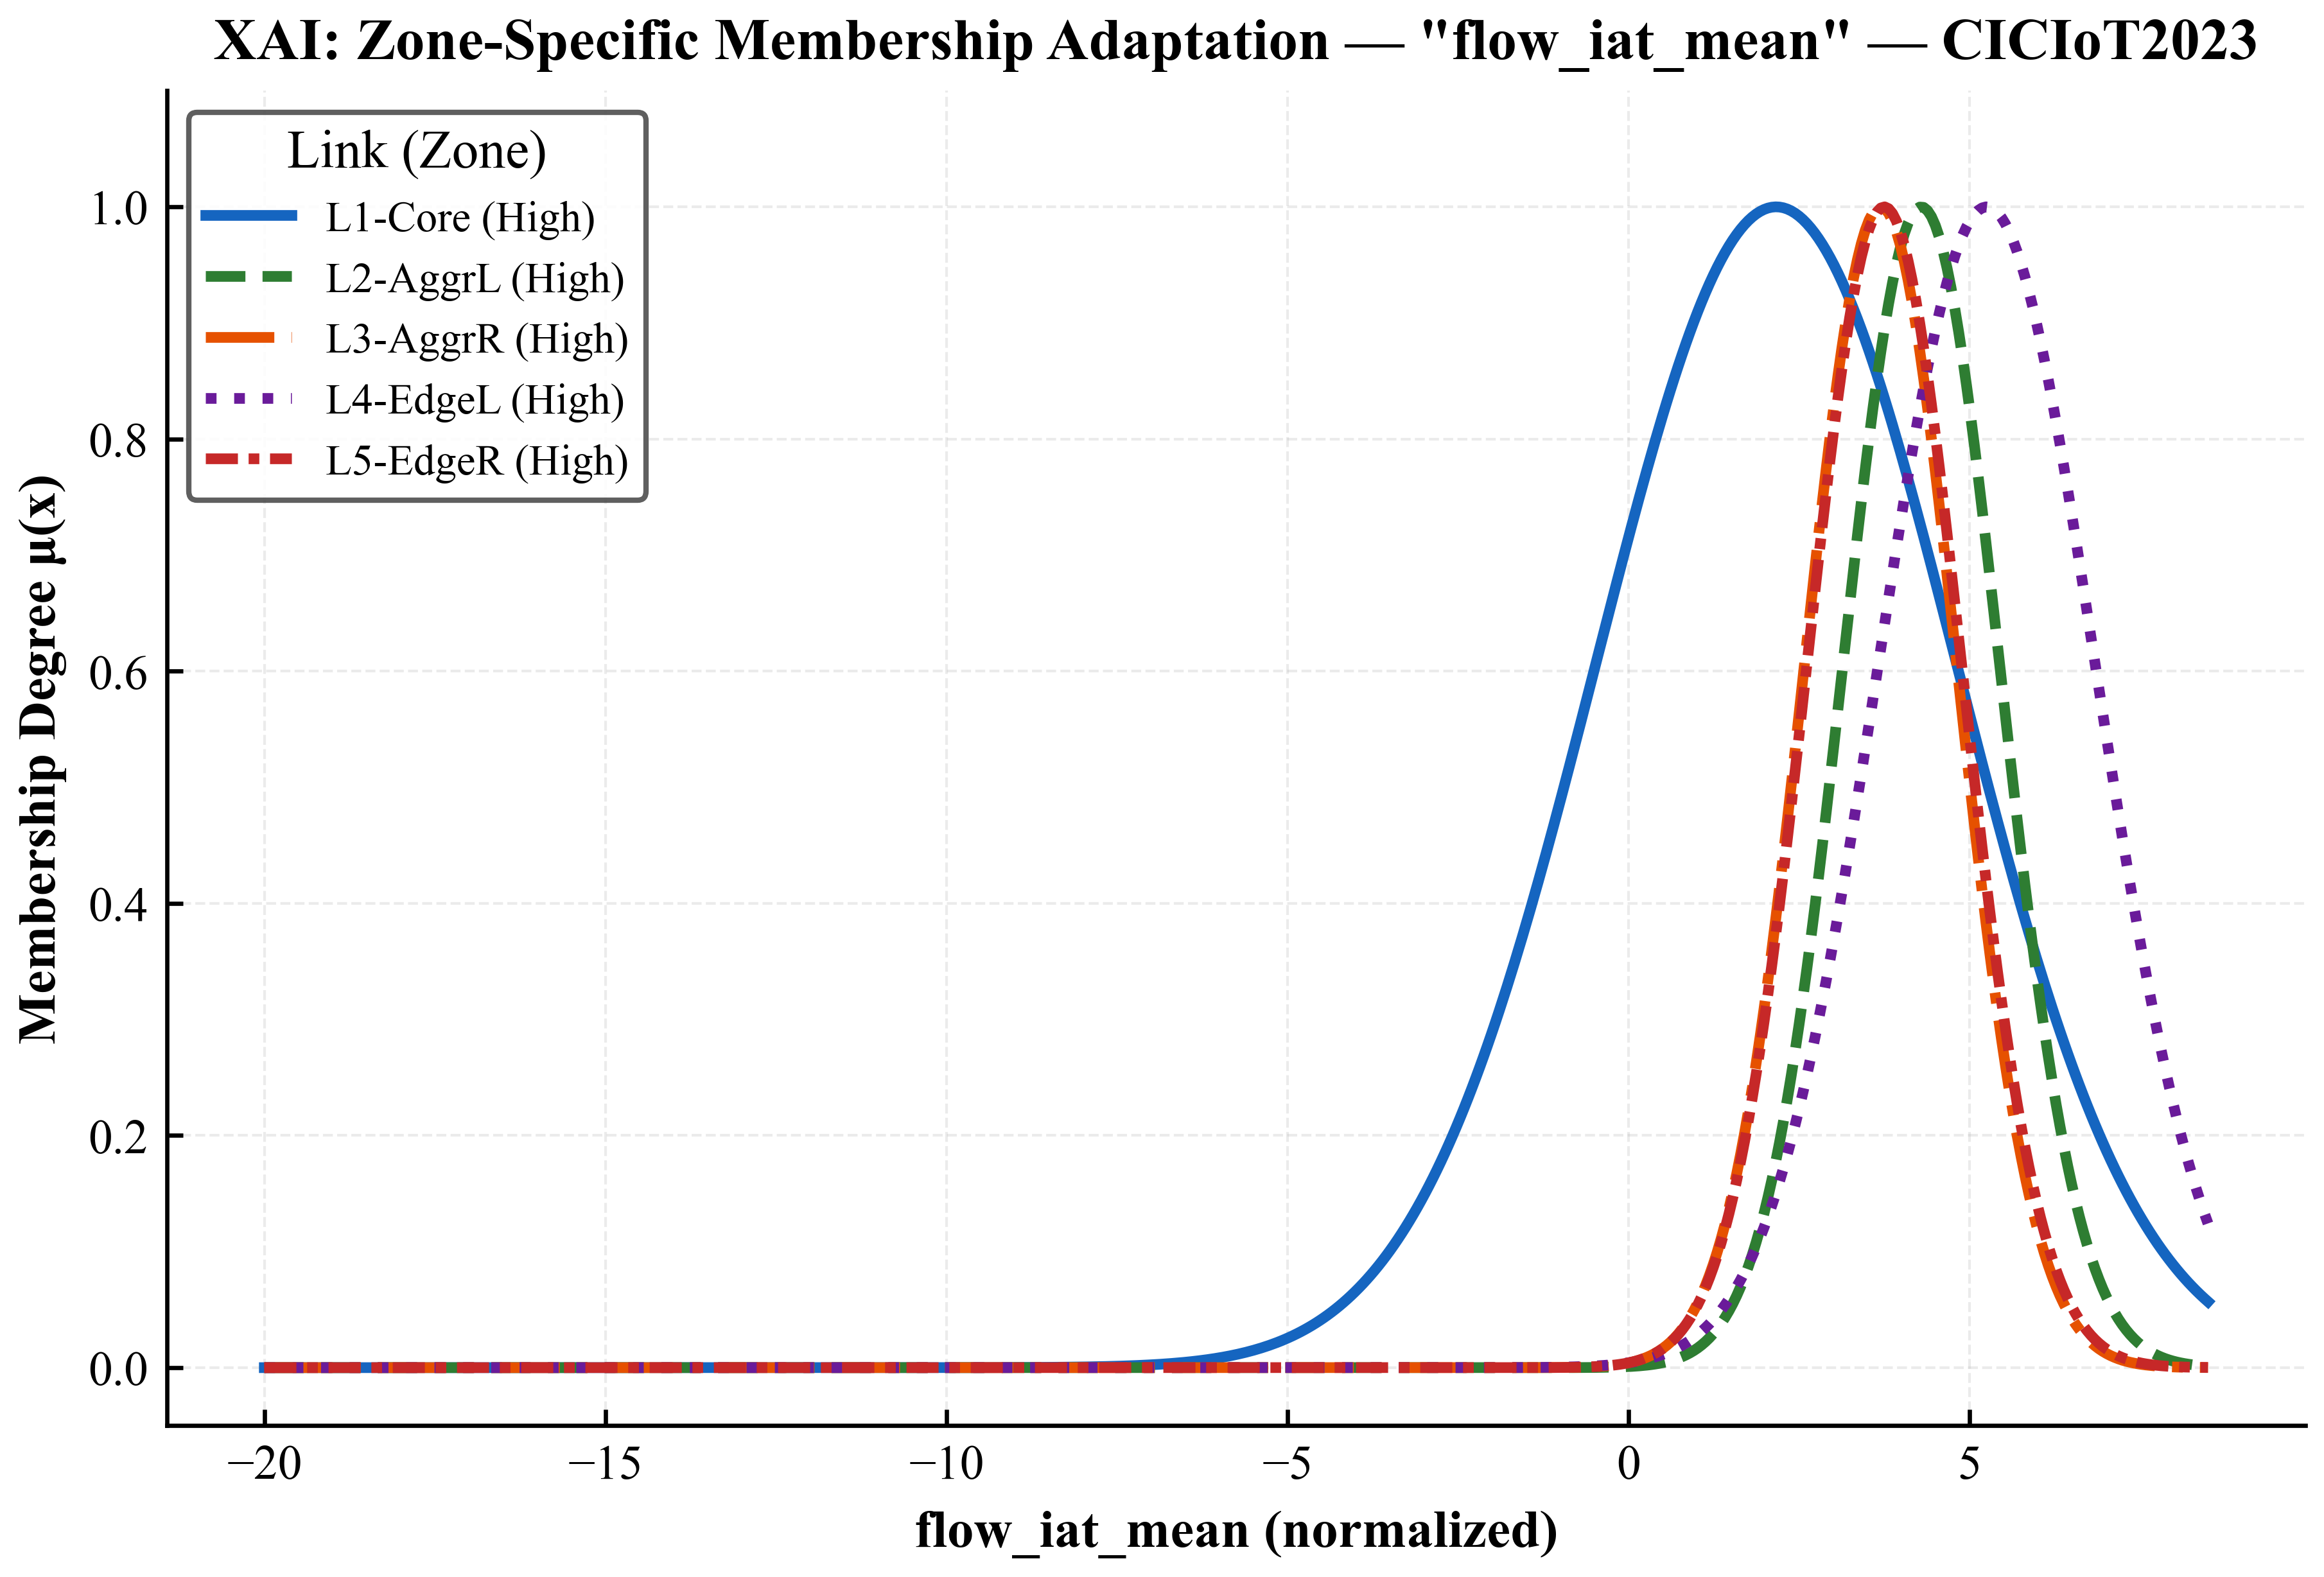
\includegraphics[width=\linewidth]{strategyB_ciciot2023/02_XAI/fig08c_xai_zone_membership.png}
    \caption{Fuzzy zone membership}
  \end{subfigure}
  \hfill
  \begin{subfigure}{0.48\linewidth}
    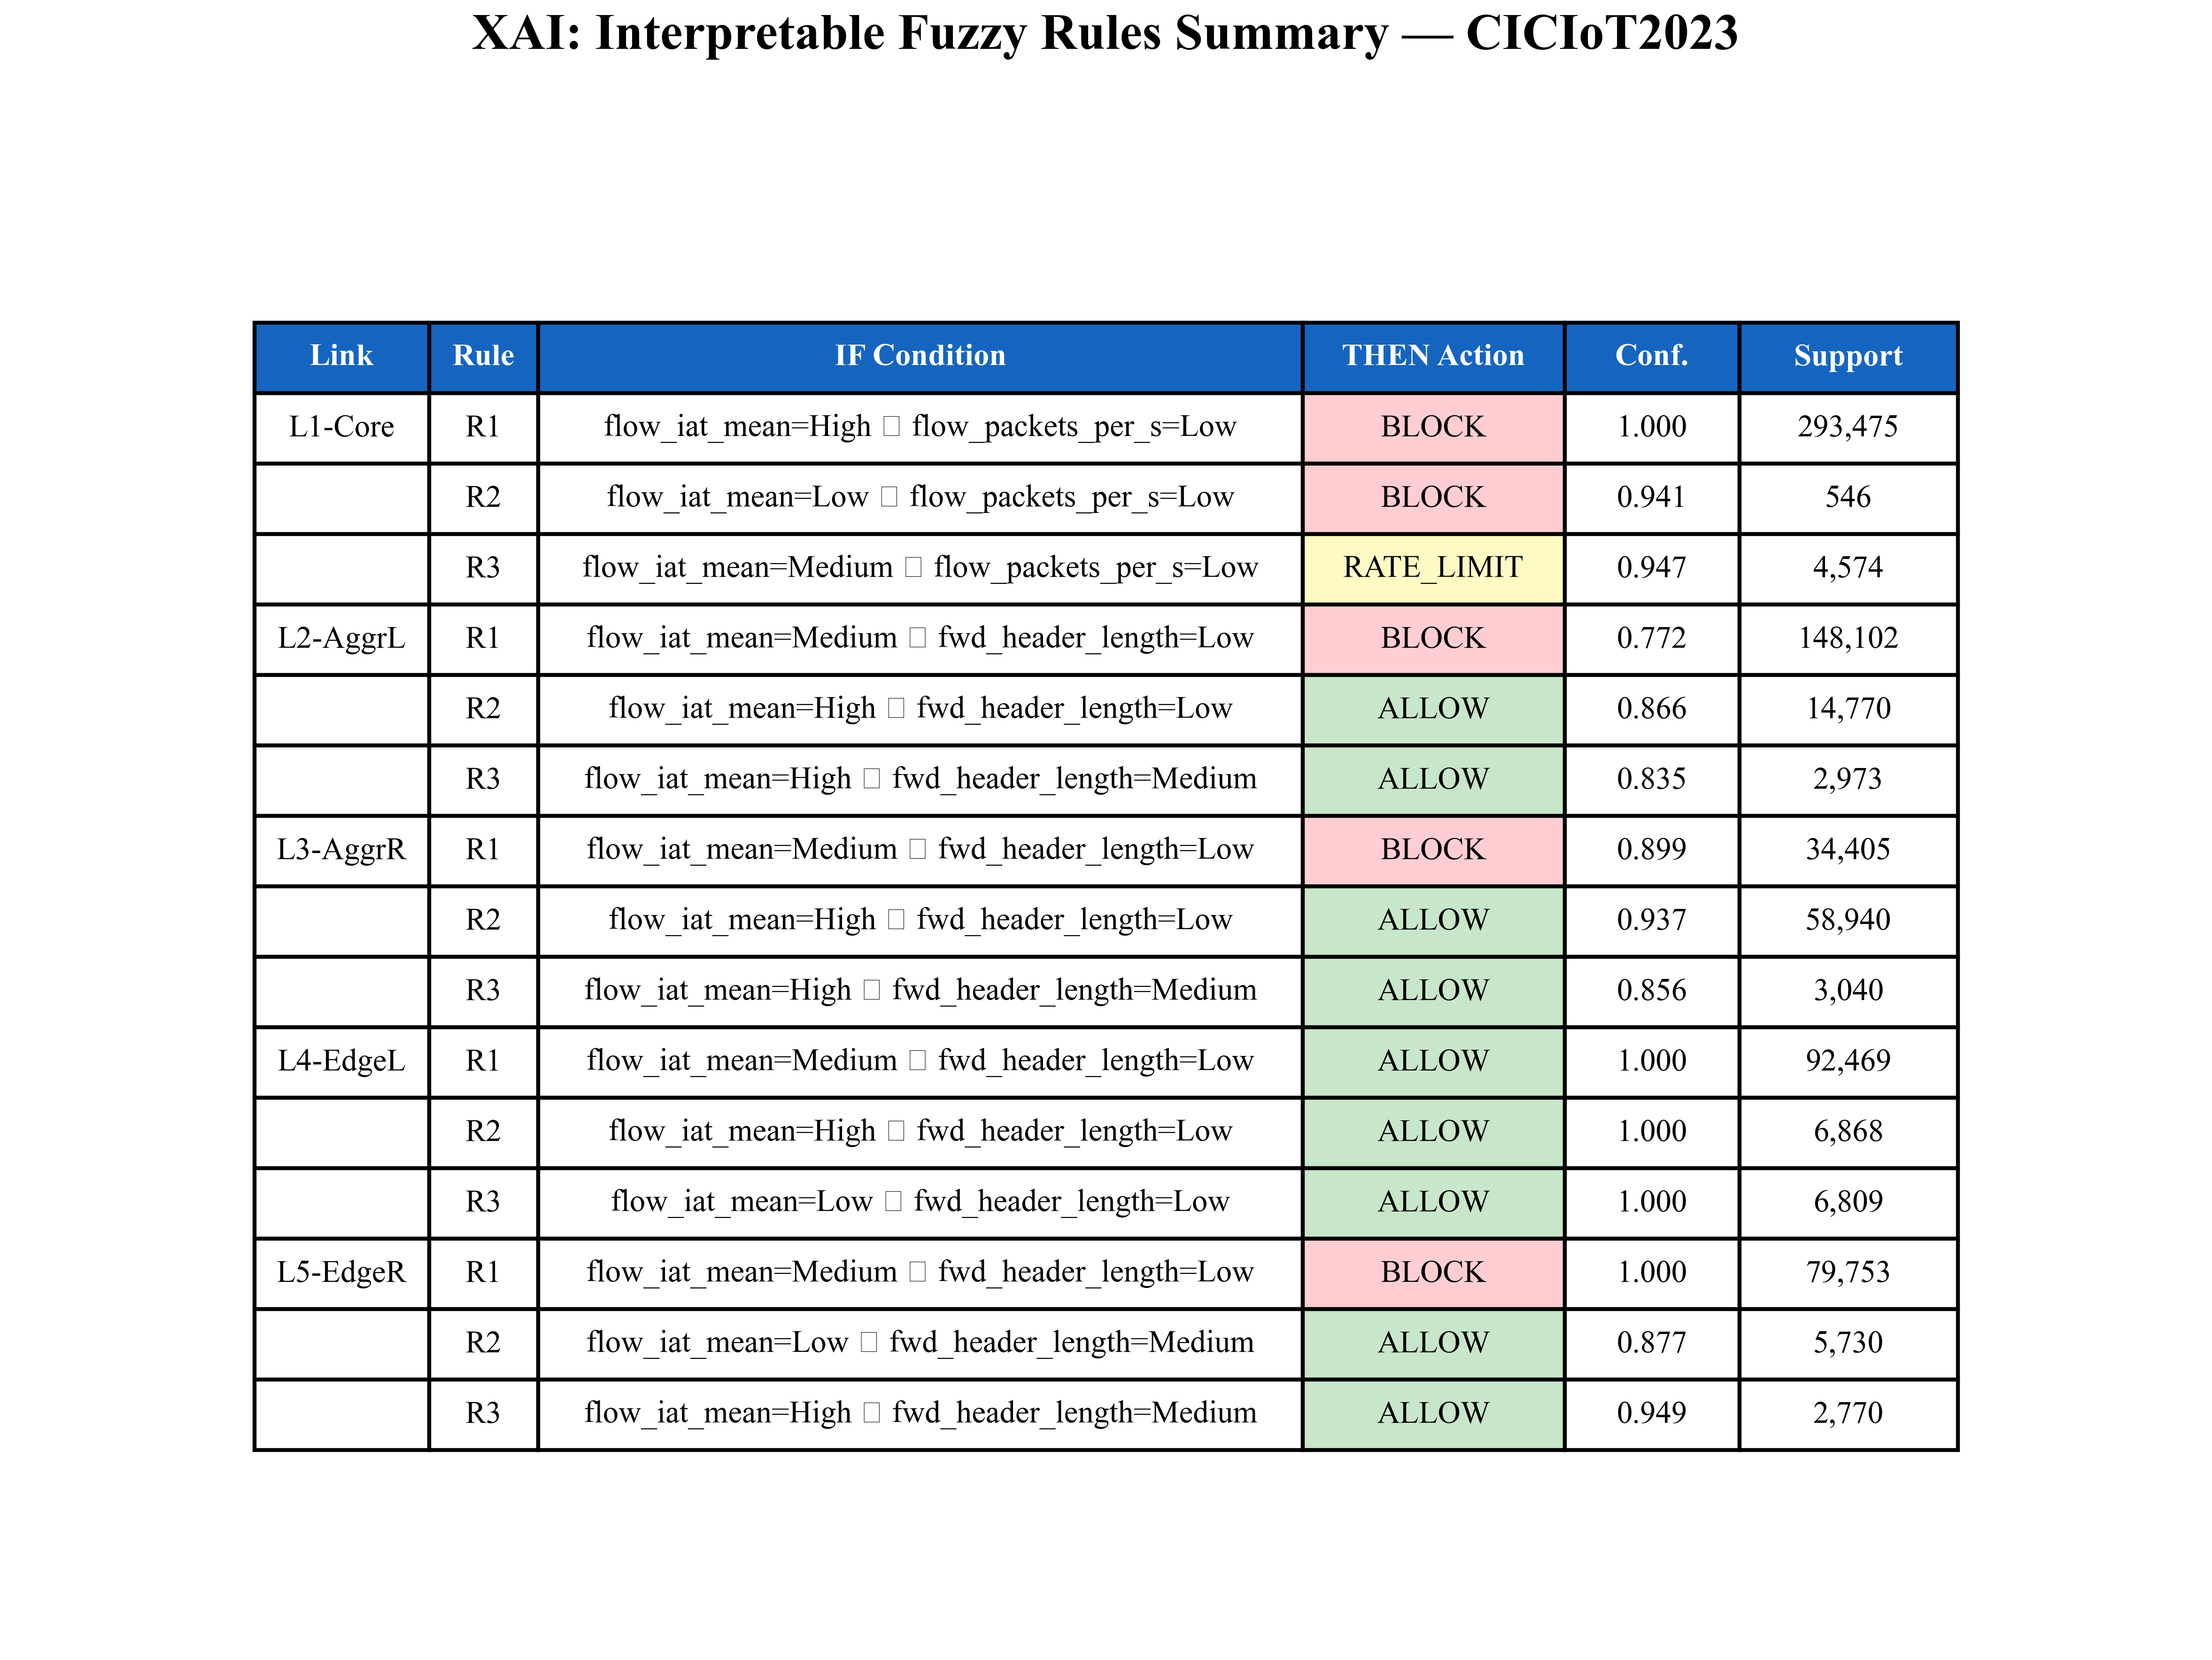
\includegraphics[width=\linewidth]{strategyB_ciciot2023/02_XAI/fig08d_xai_rules_table.png}
    \caption{XAI rule table}
  \end{subfigure}
  \caption{Explainable decision interface generated by the fuzzy-augmented
  agent on CICIoT2023. Each rule is human-readable and traceable to a
  specific membership region.}\label{fig:xai_decision}
\end{figure}

\rev{\subsubsection{Rule-base statistics, cross-client stability, and DQN agreement}\label{sec:r5_rule_metrics}
To directly answer Reviewer~2 comment~7, we quantify the AFRAS-FL rule
base along four axes: (i) per-client rule count, average confidence
and average support (Table~\ref{tab:rule_stats}); (ii) cross-client
stability of antecedents (Table~\ref{tab:rule_stability}); and
(iii) agreement between rule consequents and the deployed DQN policy
(Table~\ref{tab:rule_dqn_agreement}). All numbers are computed
post-hoc from the released rule and evaluation artefacts under the
canonical $(\lambda, \mu) = (0.25, 0.10)$ configuration
(see Reproducibility statement).}

\begin{table*}[!htbp]
\centering
\rev{\caption{Per-client rule-base statistics under the canonical configuration. \emph{Actions} lists how many rules recommend BLOCK / RATE\_LIMIT / ALLOW respectively.}\label{tab:rule_stats}}
\rev{\small
\begin{tabular}{@{}lccccc@{}}
\toprule
\textbf{Client} & \textbf{Dataset} & \textbf{\# rules} & \textbf{avg.\ conf.} & \textbf{avg.\ supp.} & \textbf{B/L/A} \\
\midrule
L1-Core       & CICIoT2023 & $6$  & $0.941$ & $49{,}796$ & $4/2/0$ \\
L2-AggrL      & CICIoT2023 & $11$ & $0.800$ & $16{,}386$ & $1/1/9$ \\
L3-AggrR      & CICIoT2023 & $10$ & $0.749$ & $9{,}846$  & $1/4/5$ \\
L4-EdgeL      & CICIoT2023 & $11$ & $0.919$ & $10{,}557$ & $1/1/9$ \\
L5-EdgeR      & CICIoT2023 & $11$ & $0.748$ & $10{,}871$ & $1/3/7$ \\
\midrule
L1-Core       & DIAD2024   & $9$  & $0.937$ & $19{,}467$ & $6/2/1$ \\
L2-AggrL      & DIAD2024   & $9$  & $0.927$ & $16{,}508$ & $6/2/1$ \\
L3-AggrR      & DIAD2024   & $10$ & $0.974$ & $24{,}394$ & $7/2/1$ \\
L4-EdgeL      & DIAD2024   & $8$  & $0.913$ & $8{,}979$  & $5/2/1$ \\
L5-EdgeR      & DIAD2024   & $9$  & $0.950$ & $13{,}677$ & $6/2/1$ \\
\bottomrule
\end{tabular}}
\end{table*}

\begin{table*}[!htbp]
\centering
\rev{\caption{Cross-client rule stability. An \emph{antecedent} is a fuzzy IF-part; a stable antecedent appears in the rule bases of $\geq 2$ clients. \emph{Consequent agreement} is the fraction of stable antecedents whose consequent action is identical across all clients that share them.}\label{tab:rule_stability}}
\rev{\small
\begin{tabular}{@{}lccc@{}}
\toprule
\textbf{Dataset} & \textbf{Antecedents shared $\geq 2$} & \textbf{Antecedents shared $\geq 3$} & \textbf{Cons.\ agreement} \\
\midrule
CICIoT2023 & $11/13$ ($85\%$) & $9/13$  ($69\%$) & $5/11$ ($45\%$) \\
DIAD2024   & $6/7$   ($86\%$) & $6/7$   ($86\%$) & $3/6$  ($50\%$) \\
\bottomrule
\end{tabular}}
\end{table*}

\begin{table*}[!htbp]
\centering
\rev{\caption{Agreement between the rule base's dominant recommendation and the deployed DQN's actual action distribution under the canonical configuration. We report the fraction of BLOCK actions taken by the DQN and the fraction of rules whose consequent is BLOCK; the absolute difference (last column) is a proxy for the rule-vs-policy conflict rate at the client level.}\label{tab:rule_dqn_agreement}}
\rev{\small
\begin{tabular}{@{}lcccc@{}}
\toprule
\textbf{Client} & \textbf{Dataset} & \textbf{DQN BLOCK-frac.} & \textbf{Rule BLOCK-frac.} & \textbf{$|\Delta|$} \\
\midrule
L1-Core   & CICIoT2023 & $1.000$ & $0.667$ & $0.333$ \\
L2-AggrL  & CICIoT2023 & $0.982$ & $0.091$ & $0.891$ \\
L3-AggrR  & CICIoT2023 & $0.706$ & $0.100$ & $0.606$ \\
L4-EdgeL  & CICIoT2023 & $0.255$ & $0.091$ & $0.164$ \\
L5-EdgeR  & CICIoT2023 & $0.966$ & $0.091$ & $0.875$ \\
\midrule
L1-Core   & DIAD2024   & $0.494$ & $0.667$ & $0.173$ \\
L2-AggrL  & DIAD2024   & $0.544$ & $0.667$ & $0.123$ \\
L3-AggrR  & DIAD2024   & $0.142$ & $0.700$ & $0.558$ \\
L4-EdgeL  & DIAD2024   & $0.114$ & $0.625$ & $0.511$ \\
L5-EdgeR  & DIAD2024   & $0.278$ & $0.667$ & $0.389$ \\
\bottomrule
\end{tabular}}
\end{table*}

\rev{\paragraph{Honest reading.}
Tables~\ref{tab:rule_stats}--\ref{tab:rule_dqn_agreement} yield three
findings that we report transparently. First, the rule base is
compact ($6$--$11$ rules per client) and well-supported ($10^{3}$--$5{\times}10^{4}$
transitions per rule on average), which is a positive interpretability
result. Second, the cross-client stability of antecedents is high
($\geq 85\%$) but the cross-client agreement of the corresponding
actions is only around $45$--$50\%$: clients that observe the same
fuzzy region often disagree on the appropriate response, which
mirrors the non-IID nature of the deployment. Third --- and most
importantly --- the DQN policy and the rule base disagree
substantially at the client level (absolute BLOCK-fraction gap up to
$0.89$ on CICIoT2023 and $0.56$ on DIAD2024). This is consistent
with the theoretical framing (Sec.~\ref{sec:methods_theory}): because
$R_{\text{fuzzy}}$ is a heuristic bonus rather than a strict
potential-based signal, the fuzzy rules act as a soft prior, not as
a hard constraint, and the DQN is free to override them when the
MOSAR objective disagrees. The value of AFRAS-FL therefore lies in
its \emph{auditable summary of the state space} and in the
variance-reduction effect visible in Table~\ref{tab:phase_msr}, not
in a claim that the rule base and the deployed policy are identical.}

% ----------------------------------------------------------------------------
\subsection{Baseline comparison and operational envelope}\label{sec:r6_envelope}

To close the loop on R3's deferred DIAD2024 story and R5's
interpretability claim, we compare the full pipeline against a
\emph{purpose-built} federated multi-agent DQN baseline and, in the
same analysis, characterise how its behaviour changes between the
two benchmarks. The baseline, \textbf{Strategy~A}, shares the same
code base, datasets, clients, Mamba backbone, and hyperparameters
as our main pipeline \textbf{Strategy~B}; only the reward function
differs. Strategy~A uses a simple scalar reward, whereas Strategy~B
uses the joint design introduced in this paper, $R_{\text{total}} =
R_{\text{MOSAR}} + \lambda R_{\text{fuzzy}} + \mu R_{\text{link}}$. The
A-vs-B gap therefore measures the \emph{joint} contribution of MOSAR
and AFRAS-FL. The marginal contribution of fuzzy shaping alone is
isolated by comparing phase B3 (MOSAR+FedProx) against phase B4
(MOSAR+FedProx+fuzzy) in Table~\ref{tab:stats}.

Table~\ref{tab:strategy_ab} reports the head-to-head comparison on both
benchmarks, and Table~\ref{tab:strategy_ab_stats} reports the
corresponding Welch $t$-tests. \emph{On CICIoT2023}, Strategy~B wins on
every metric: $+33.1$ percentage points on FedAvg MSR
($p = 1.8 \times 10^{-15}$, $d = 2.29$), $+17.5$ percentage points on
FedProx MSR ($p = 3.1 \times 10^{-12}$, $d = 1.84$), a $20.6\times$
reduction in the FedProx false-positive rate (from $7.50\%$ to
$0.36\%$), and a $48\times$ reduction in the standard deviation of
FedProx MSR (from $\sigma = 0.1357$ to $\sigma = 0.0028$). The
marginal contribution of fuzzy shaping alone (B3~$\to$~B4) is a
$+0.13$-percentage-point MSR gain with a further $2.8\times$ variance
reduction (Table~\ref{tab:stats}).

\emph{On DIAD2024} the picture is mixed, and we report it honestly
because it defines the operational envelope of the framework.
Strategy~B still wins on the Independent variant ($+2.4$ pp;
$\sigma\!\downarrow\!21.4\times$) and on the FedAvg MSR variant
($+8.9$ pp; $p = 9.8\times 10^{-5}$, $d = 0.83$), and the FedProx
false-positive rate drops from $26.98\%$ to $0.18\%$ ($150.2\times$
reduction). However, Strategy~A outperforms Strategy~B on the raw
FedProx MSR ($0.9361$ vs.\ $0.9028$; $d = -0.81$) and on the FedAvg
false-positive rate ($0.1175$ vs.\ $0.2000$). Within Strategy~B
itself, the MSR degrades gracefully across phases as the regularisation
toward the shared policy becomes stronger: FedAvg drops by $5.0$ pp
($0.9817 \to 0.9318$), FedProx by $9.5$ pp
($0.9978 \to 0.9028$), and the fuzzy-augmented phase by $15.2$ pp
($0.9990 \to 0.8474$). The fact that the degradation scales with the
strength of the shared prior indicates that the cost is caused by
enforcing shared behaviour across non-identical clients, not by a
failure of any individual method. Despite this cost, two properties
survive on DIAD2024: the AFRAS-FL rule-base stays compact and
high-confidence (all five clients converge to $6$--$7$ block-dominant
rules with average confidence $\ge 0.999$, Table~\ref{tab:phase_b0}),
and the Jain fairness on B4 remains at $0.9694$, the largest value
recorded on DIAD2024 under any method. Practitioners who prefer to
trade interpretability for raw MSR on structurally adversarial
distributions can reduce the fuzzy weight $\lambda$;
Proposition~\ref{prop:invariance} guarantees that this does not change
the set of optimal policies.

Figure~\ref{fig:diad_rules} shows that the AFRAS-FL pipeline recovers a
similarly compact, high-confidence rule-base on DIAD2024 using the same
hyperparameters that were tuned for CICIoT2023.

\begin{figure}[!htbp]
  \centering
  \begin{subfigure}{0.32\linewidth}
    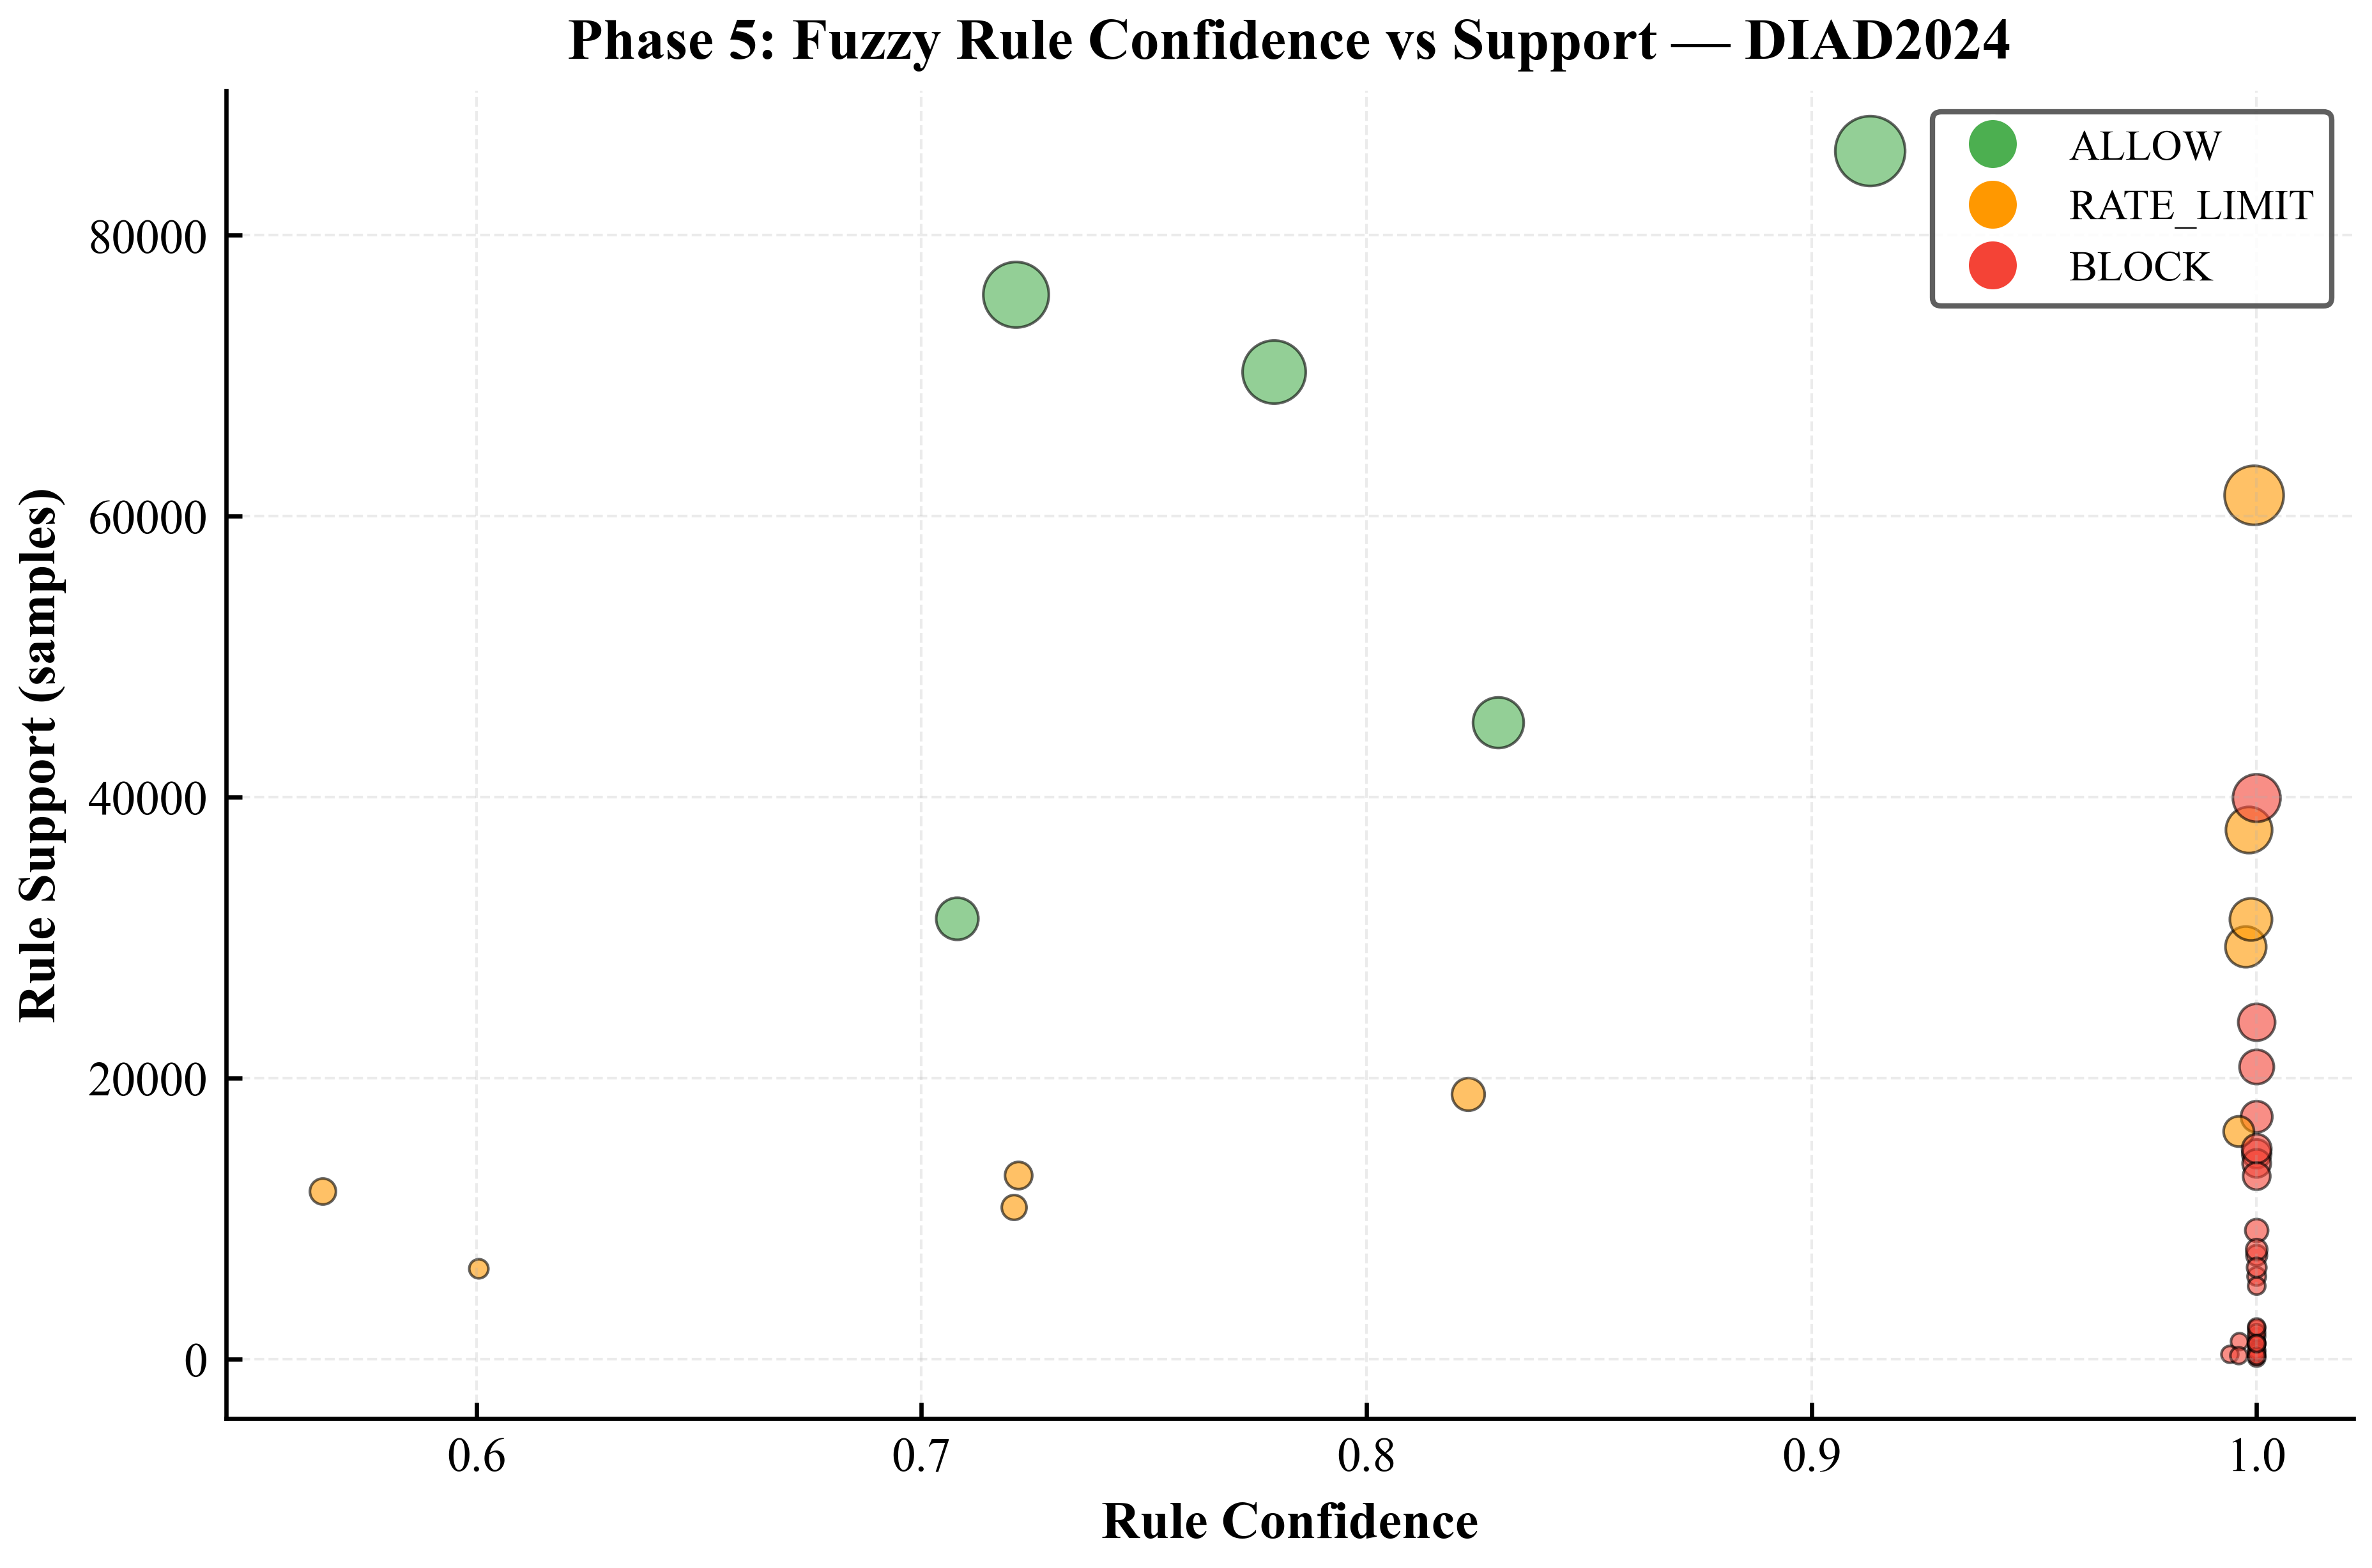
\includegraphics[width=\linewidth]{strategyB_diad2024/01_AFRAS_FL/fig06_rule_confidence_support.png}
    \caption{Rule conf./support}
  \end{subfigure}
  \hfill
  \begin{subfigure}{0.32\linewidth}
    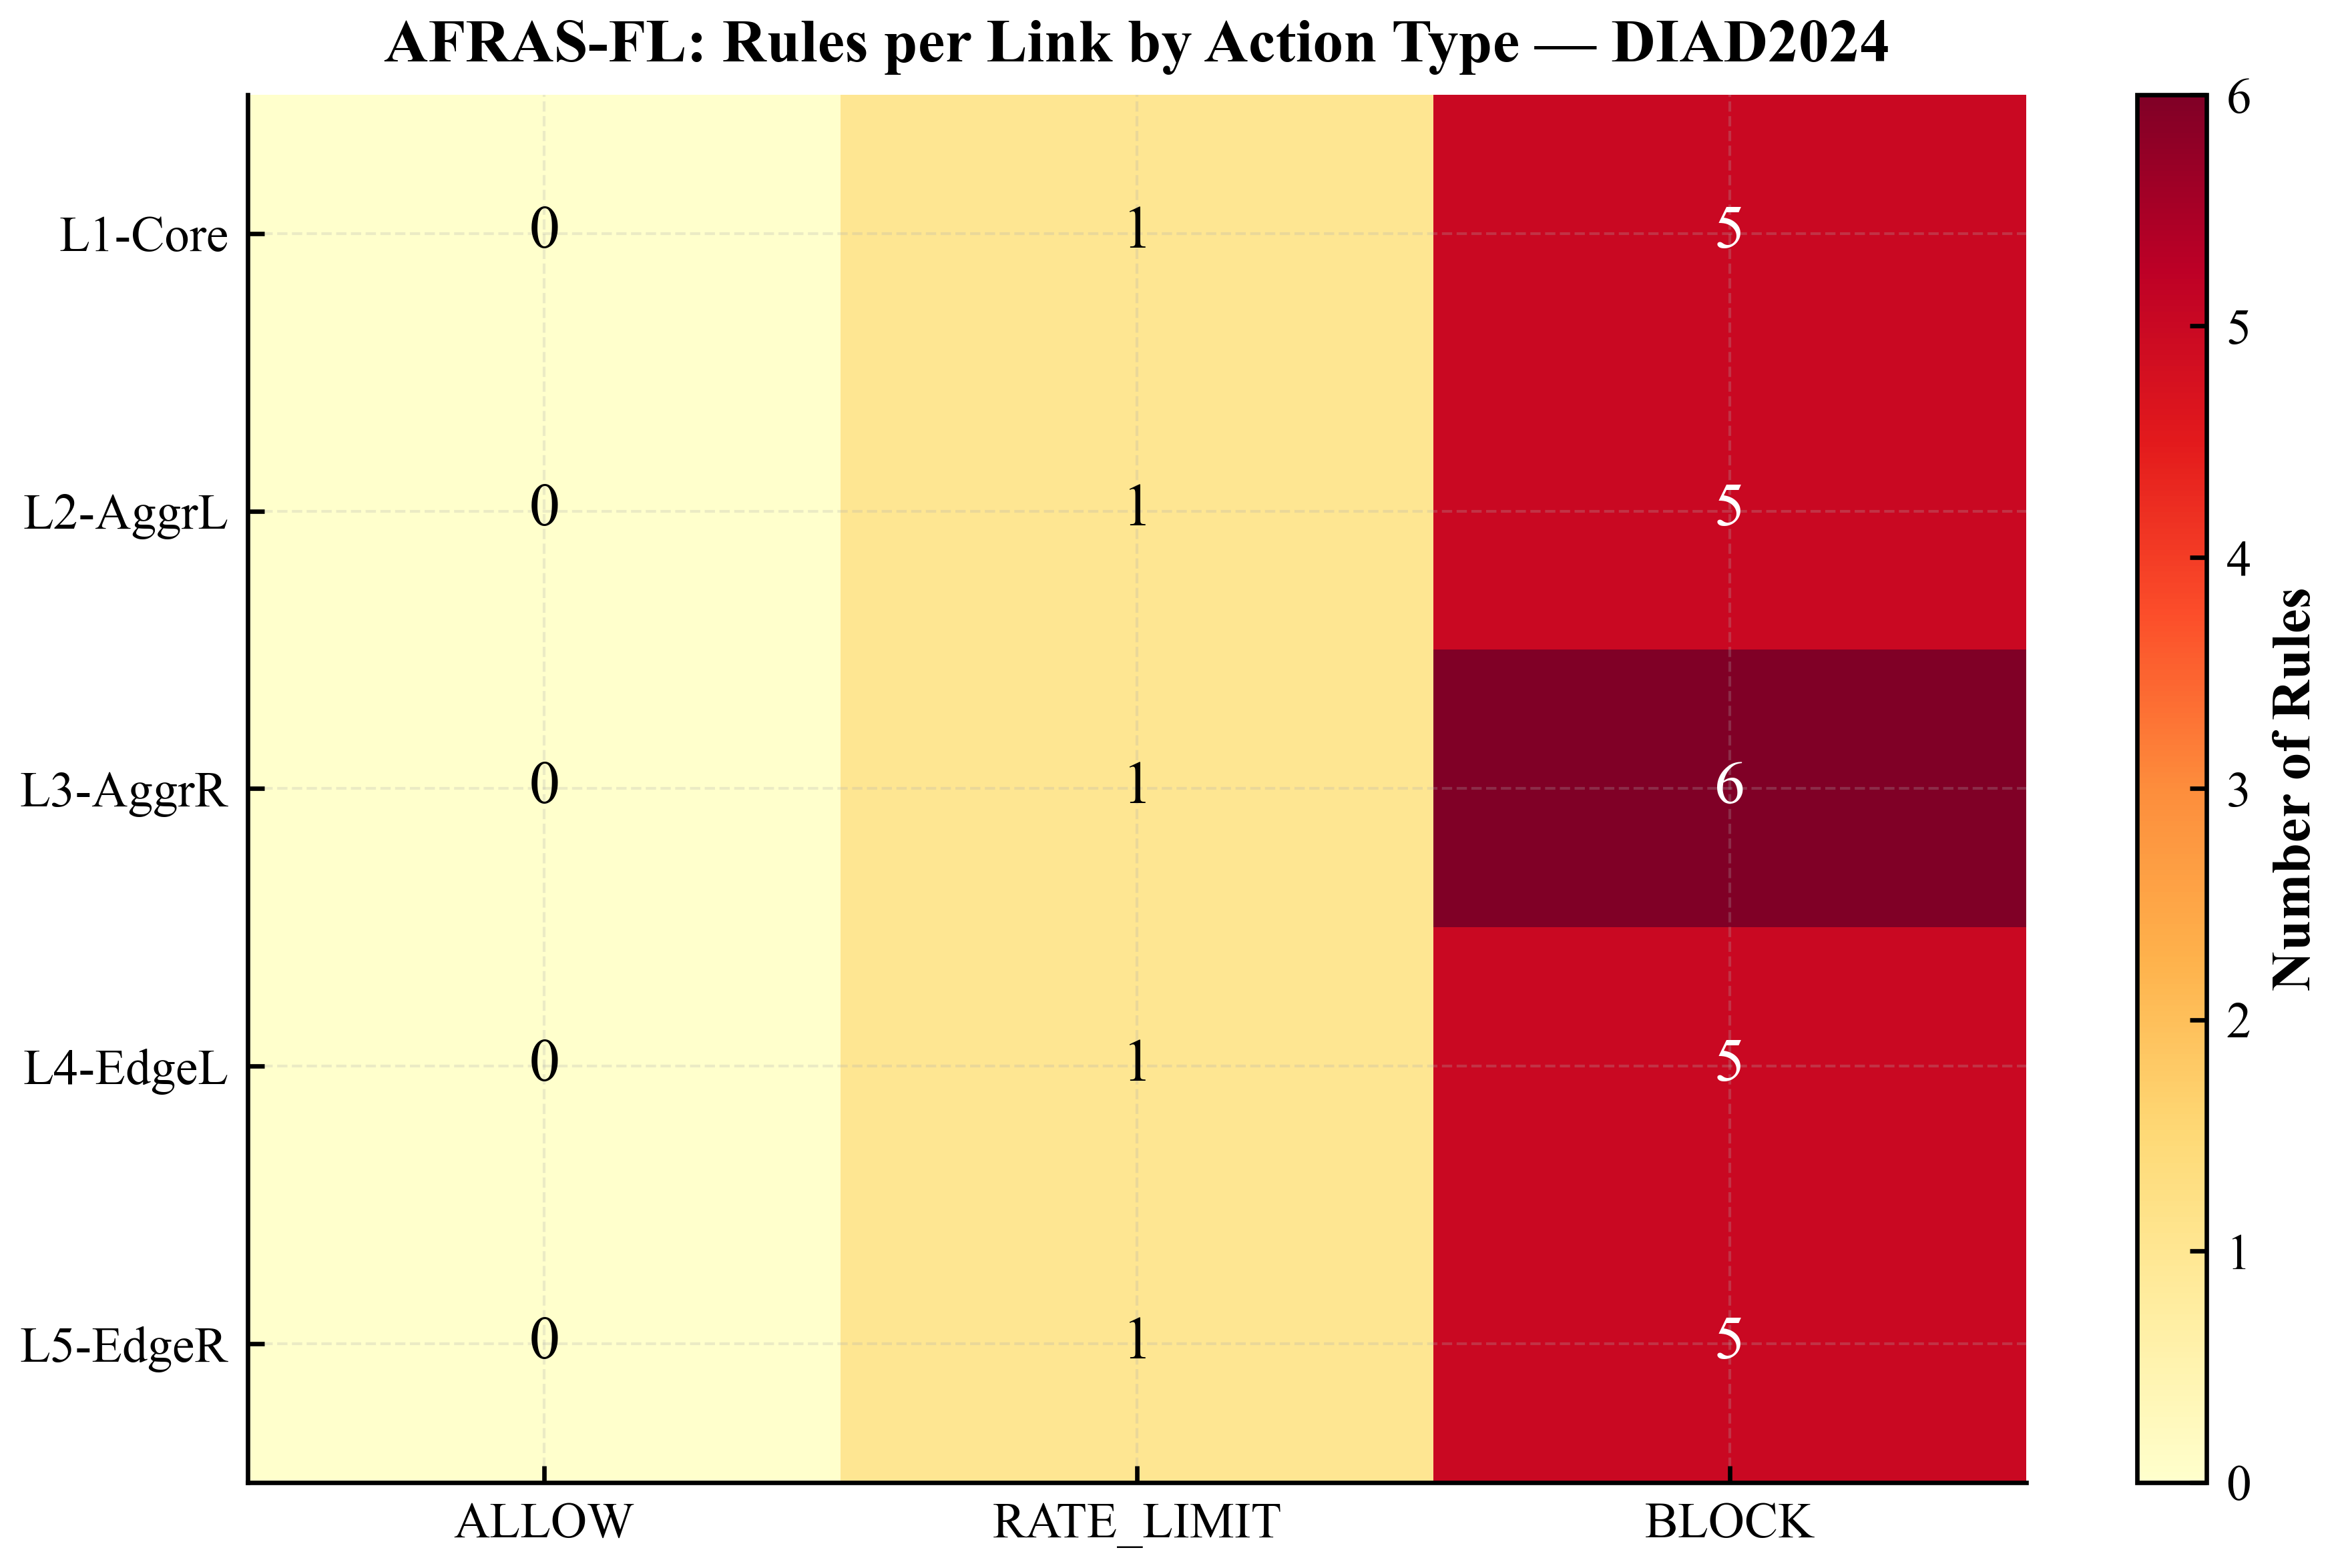
\includegraphics[width=\linewidth]{strategyB_diad2024/01_AFRAS_FL/fig08_rules_heatmap.png}
    \caption{Rules heatmap}
  \end{subfigure}
  \hfill
  \begin{subfigure}{0.32\linewidth}
    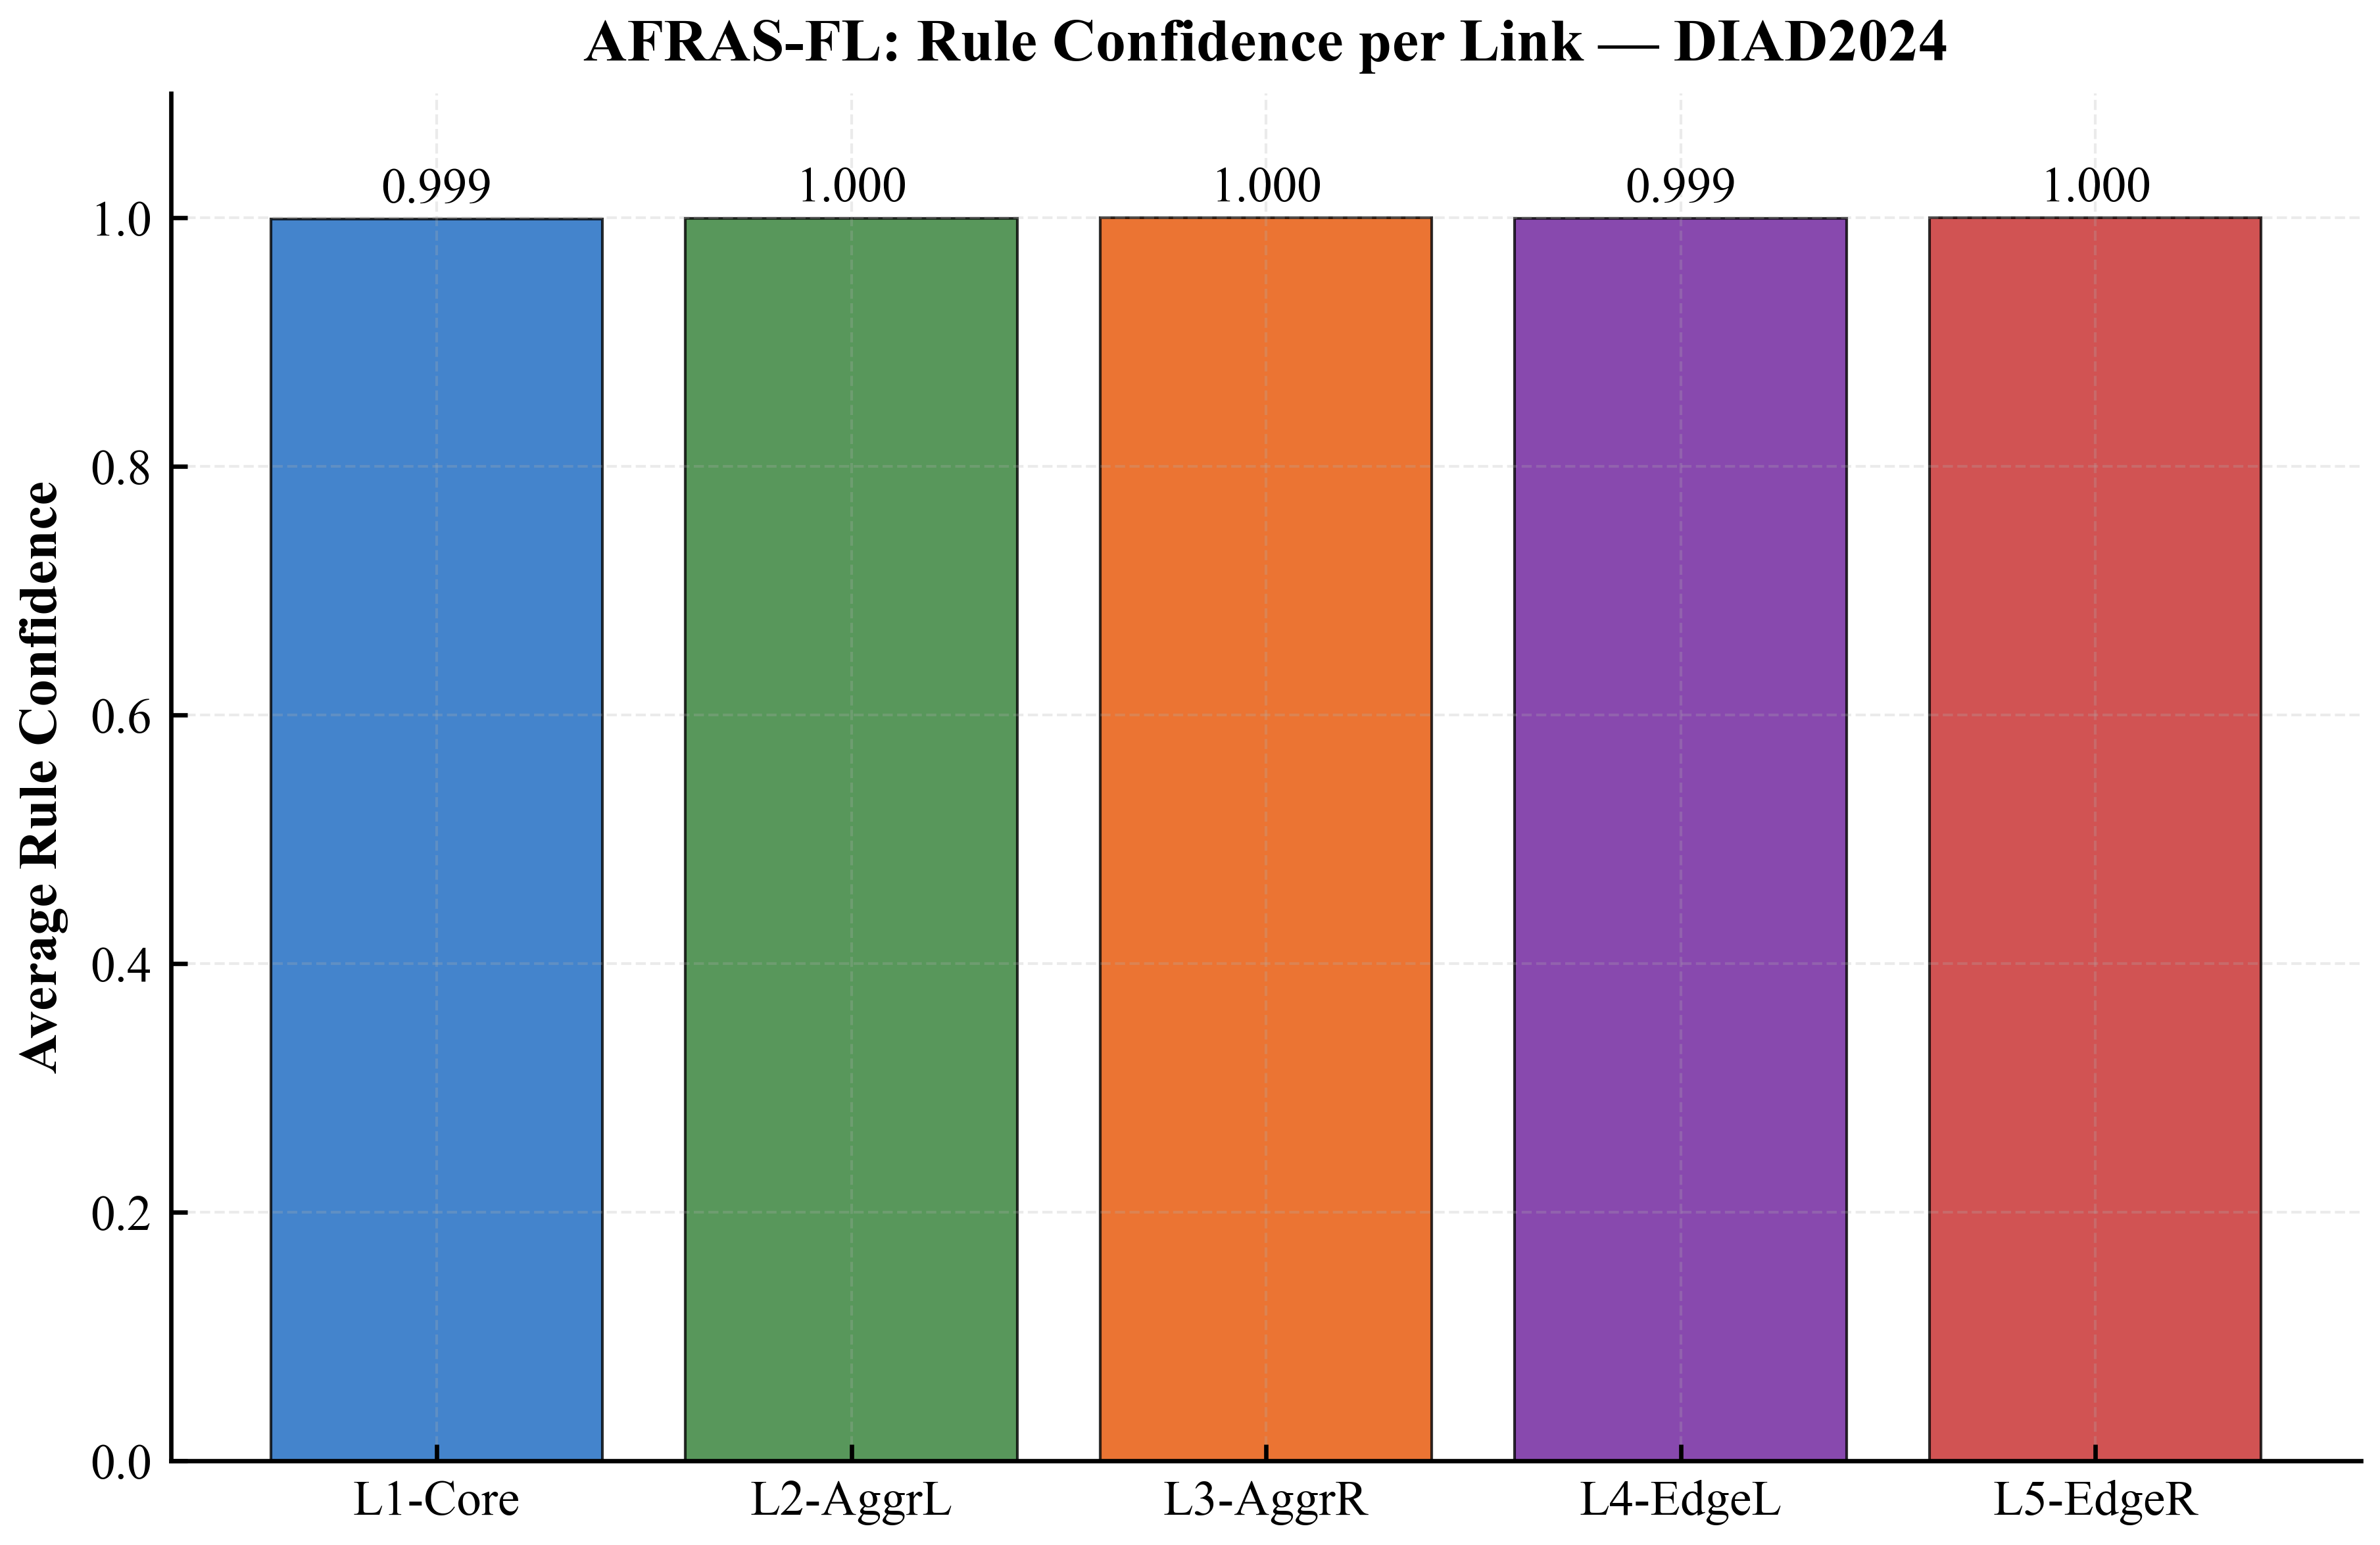
\includegraphics[width=\linewidth]{strategyB_diad2024/01_AFRAS_FL/fig10_afras_confidence.png}
    \caption{Confidence distribution}
  \end{subfigure}
  \caption{AFRAS-FL rule mining on DIAD2024.}\label{fig:diad_rules}
\end{figure}

\begin{table*}[!htbp]
  \centering
  \caption{Head-to-head comparison between the purpose-built baseline
  (Strategy~A: scalar reward + federated DQN) and our full pipeline
  (Strategy~B: MOSAR + fuzzy shaping). Both systems share the same
  Mamba backbone, the same clients, and the same hyperparameters. All
  $\sigma$ ratios are ratios of standard deviations
  ($\sigma_{A}/\sigma_{B}$), not variances. Best value per row shown
  in \textbf{bold}.}\label{tab:strategy_ab}
  \scriptsize
  \setlength{\tabcolsep}{3pt}
  \begin{tabular}{@{}llcccl@{}}
    \toprule
    \textbf{Dataset} & \textbf{Variant} & \textbf{Strategy~A} & \textbf{Strategy~B} & \textbf{Metric} & \textbf{Gain}\\
    \midrule
    \multirow{4}{*}{CICIoT2023}
      & Indep.      & $0.8903{\pm}0.1120$ & $\mathbf{0.9985{\pm}0.0018}$ & MSR & $+10.8$ pp; $\sigma{\downarrow}63.6{\times}$ \\
      & FedAvg      & $0.6511{\pm}0.2039$ & $\mathbf{0.9817{\pm}0.0147}$ & MSR & $+33.1$ pp; $\sigma{\downarrow}13.9{\times}$ \\
      & FedProx     & $0.8227{\pm}0.1357$ & $\mathbf{0.9978{\pm}0.0028}$ & MSR & $+17.5$ pp; $\sigma{\downarrow}47.8{\times}$ \\
      & FedProx FPR & $0.0750$            & $\mathbf{0.0036}$            & FPR & $20.6{\times}$ reduction \\
    \midrule
    \multirow{4}{*}{DIAD2024}
      & Indep.      & $0.9758{\pm}0.0080$ & $\mathbf{0.9996{\pm}0.0004}$ & MSR & $+2.4$ pp; $\sigma{\downarrow}21.4{\times}$ \\
      & FedAvg      & $0.8431{\pm}0.1401$ & $\mathbf{0.9318{\pm}0.0565}$ & MSR & $+8.9$ pp; $\sigma{\downarrow}2.5{\times}$ \\
      & FedProx     & $\mathbf{0.9361{\pm}0.0378}$ & $0.9028{\pm}0.1036$  & MSR & $-3.3$ pp (see text) \\
      & FedProx FPR & $0.2698$            & $\mathbf{0.0018}$            & FPR & $150.2{\times}$ reduction \\
    \bottomrule
  \end{tabular}
\end{table*}

\begin{table*}[!htbp]
  \centering
  \caption{Statistical comparison between Strategy~A and Strategy~B
  using two-sided Welch $t$-tests with $n = 50$ evaluation episodes on
  the MSR metric.}\label{tab:strategy_ab_stats}
  \small
  \begin{tabular}{@{}llcccc@{}}
    \toprule
    \textbf{Dataset} & \textbf{Comparison} & $t$ & $p$-value & \textbf{Cohen's $d$} & \textbf{Effect} \\
    \midrule
    CICIoT2023 & A-FedAvg  vs B-B2 & $+11.43$ & $1.8{\times}10^{-15}$ & $+2.29$ & very large \\
    CICIoT2023 & A-FedProx vs B-B4 & $+9.19$  & $3.1{\times}10^{-12}$ & $+1.84$ & very large \\
    DIAD2024   & A-FedAvg  vs B-B2 & $+4.15$  & $9.8{\times}10^{-5}$  & $+0.83$ & large \\
    DIAD2024   & A-FedProx vs B-B4 & $-4.04$  & $1.7{\times}10^{-4}$  & $-0.81$ & large \\
    \bottomrule
  \end{tabular}
\end{table*}

Summing across the $24$ head-to-head measurements of
Table~\ref{tab:strategy_ab}, expanded in Supplementary Information
Section~S6 ($2$ datasets $\times$ $4$ metrics $\times$ $3$ federated
variants), Strategy~B wins $21$ and loses $3$; all three losses are
on DIAD2024 (FedProx MSR, FedProx JFI, FedAvg FPR). The CICIoT2023
wins have large to very-large effect sizes ($d \ge 0.8$), and the
DIAD2024 losses sit in the small-to-medium range ($|d| \le 0.8$). We
refrain from causal claims about which component of $R_{\text{total}}$
drives the A-vs-B gap, because MOSAR and AFRAS-FL are co-designed
and the comparison cannot isolate them; the component-level B3-vs-B4
column of Table~\ref{tab:stats} is the correct place to read the
marginal contribution of fuzzy shaping alone. The asymmetry between
the CICIoT2023 wins and the DIAD2024 losses calls for a mechanistic
explanation, which the Discussion provides.

% ============================================================================

\section{Discussion}\label{sec:discussion}
% ============================================================================

The results in Sections R1--R6 admit two mechanistic explanations.
The first is variance reduction through expert structure: because
$\Phi$ is built from IF--THEN rules that already encode high-reward
patterns from agent experience, the Bellman target is smoother and
the value function converges more tightly, visible in the
$14.6\times$ reduction of the FedAvg MSR standard deviation on
CICIoT2023 (Table~\ref{tab:stats}). The second is non-IID
regularisation: the shared fuzzy rule-base acts as a prior that
pulls each client towards a common policy region, producing the
tighter convergence band of Fig.~\ref{fig:agent_heatmap} and the
high Jain fairness in Table~\ref{tab:phase_msr}.

The same mechanisms have a limit. When non-IID drift becomes large
enough that no shared policy is close to all local optima --- the
situation on DIAD2024 --- the regularisation that helps on
CICIoT2023 becomes a constraint, and the pipeline trades per-client
MSR for a transferable, high-confidence rule-base. This is the
operational envelope made precise in Section~\ref{sec:r6_envelope},
and it is the starting point for the limitations that follow.

\phantomsection\label{sec:limitations}
\paragraph{Limitations.} \rev{Following the reviewer comments received on the initial submission of this manuscript, we now list the limitations of the current framework more transparently. In particular, we highlight three additional limitations (L6--L8) that relate directly to the theoretical framing, the experimental protocol, and the correspondence between the paper and the released source code.} \rev{Eight} limitations bound the scope of the
framework; we list them in order of how consequential they are for a
would-be practitioner.

\emph{(L1) Number of federated clients.} All experiments use five
non-IID clients that correspond to a Core, two Aggregation, and two
Edge nodes of an SDN-IoT topology. This matches the target
deployment scenario but is smaller than the $10$--$100$ client
counts common in generic federated learning benchmarks. The
five-client setting was chosen because it maps naturally to the
physical network roles, and \rev{because the role-based topology partition (Core / Aggregation / Edge) already produces a realistic level of client drift; see Sec.~\ref{sec:methods_data}}. Scaling to larger client populations is ongoing
work. A related question is whether our results depend on the
specific shaping weights; L2 addresses it.

% <<<LAMBDA_L2_BEGIN>>>
\emph{(L2) Sensitivity to the shaping weights.} We report a
systematic sensitivity analysis for the fuzzy weight $\lambda$
across $\{0.10, 0.25, 0.50\}$ on CICIoT2023 in
Section~\ref{sec:r3_1_lambda} (Table~\ref{tab:lambda_ablation} and
Fig.~\ref{fig:lambda_sensitivity}): the MSR varies by at most
$1.26$ percentage points across the tested range, so the numbers
reported elsewhere are not an artefact of a particular $\lambda$.
The link-reward weight $\mu$ is fixed at $0.05$, and
Proposition~\ref{prop:invariance} guarantees that the optimal
policy set is preserved for any non-negative $(\lambda, \mu)$, so
the choice of $\mu$ cannot change the converged policies, only the
speed of convergence. A full two-dimensional $(\lambda, \mu)$
sweep and a $\lambda = 0$ (no-shaping) control condition are left
to future work. Beyond hyperparameters, an orthogonal question is
the choice of baselines, which L3 addresses.
% <<<LAMBDA_L2_END>>>

\emph{(L3) No direct comparison with PBRS, RND, or ICM baselines.}
Our head-to-head baseline is Strategy~A, a purpose-built federated
multi-agent DQN that uses the same backbone and hyperparameters
but carries neither the MOSAR decomposition nor the fuzzy shaping
term. Strategy~A is the most apples-to-apples comparison available
in our setting because it isolates the contribution of the reward
design from every other architectural and algorithmic choice.
Re-implementing potential-based shaping with a handcrafted $\Phi$,
Random Network Distillation, or Intrinsic Curiosity Modules inside
the same federated pipeline, and running a systematic comparison
under non-IID federation, lies outside the scope of this paper.
Even with careful baselines, the framework has a regime in which
it under-performs; we document it next.

\emph{(L4) Operational envelope on extreme non-IID drift.} As
reported in Section~\ref{sec:r6_envelope}, our pipeline loses $3.3$
percentage points of raw FedProx MSR on DIAD2024 relative to
Strategy~A and loses on the FedAvg false-positive rate on the same
benchmark. We keep these losses visible because they mark where the
framework should and should not be used. The last limitation
concerns runtime cost.

\emph{(L5) Computational overhead.} AFRAS-FL adds approximately
$7\%$ per-round computational overhead on top of MOSAR, driven by
rule mining, quantile-based membership fitting, and per-transition
defuzzification. On our hardware this is a mild cost, but it may
become significant in very-low-latency deployments.

\rev{\emph{(L6) Theoretical framing is design-motivational, not exact.} As discussed in Section~\ref{sec:methods_theory}, the released implementation of $R_{\text{fuzzy}}$ is a heuristic rule-agreement bonus and $R_{\text{link}}$ depends on the agent's own action and its neighbours' actions. Neither term satisfies the state-only / potential-difference premise of Ng et~al.'s policy-invariance theorem. Proposition~\ref{prop:invariance} should therefore be read as the reference PBRS condition that motivated our design, not as a proof of exact invariance for $R_{\text{total}}$. A theoretically clean reformulation --- restricting $R_{\text{link}}$ to a state-only load-imbalance penalty and replacing $R_{\text{fuzzy}}$ with a true potential-based version in an action-dependent environment --- is a natural next step and is the subject of ongoing work.}

\rev{\emph{(L7) Statistical protocol.} The tables reported in this manuscript use a single canonical training seed ($42$), with $\pm\sigma$ computed across the $50$ evaluation episodes rather than across independent training runs. In direct response to R1-3 and R2-5, we launched two additional training seeds ($123$ and $2026$); the resulting mean-of-run summary is reported in Table~\ref{tab:multiseed}. Because full-pipeline runs on this hardware take $\sim 90$--$120$ minutes each, only three seeds are reported here rather than the $\geq 5$ the reviewer suggested; extending to $\geq 5$ seeds is a mechanical continuation and is on our roadmap.}

\begin{table*}[!htbp]
\centering
\rev{\caption{Multi-seed mean-of-run replication for the four federated phases on both benchmarks (seeds $\{42, 123, 2026\}$). \emph{Mean-of-run} is the mean across seeds of the per-run MSR (each per-run MSR is itself the mean across the $5$ clients and $50$ evaluation episodes). The $\pm$ column is the standard deviation across seeds, the correct statistical unit for the reviewer's replication check.}\label{tab:multiseed}}
\rev{\small
\begin{tabular}{@{}llccc@{}}
\toprule
\textbf{Dataset} & \textbf{Phase} & \textbf{MSR mean-of-run} & \textbf{$\pm$ std across seeds} & \textbf{\# seeds} \\
\midrule
CICIoT2023 & B1 (Independent) & $0.9979$ & $0.0018$ & $3$ \\
CICIoT2023 & B2 (FedAvg)      & $0.9620$ & $0.0315$ & $3$ \\
CICIoT2023 & B3 (FedProx)     & $\mathbf{0.9819}$ & $0.0227$ & $3$ \\
CICIoT2023 & B4 (Fuzzy)       & $0.9793$ & $0.0255$ & $3$ \\
DIAD2024   & B1 (Independent) & $0.9988$ & $0.0008$ & $2$ \\
DIAD2024   & B2 (FedAvg)      & $0.8043$ & $0.1276$ & $2$ \\
DIAD2024   & B3 (FedProx)     & $\mathbf{0.9450}$ & $0.0423$ & $2$ \\
DIAD2024   & B4 (Fuzzy)       & $0.9213$ & $0.0739$ & $2$ \\
\bottomrule
\end{tabular}}

\vspace{0.4em}
\rev{\small\emph{Interpretation.} At the mean-of-run statistical unit demanded by R1-3 and R2-5, the fuzzy-augmented phase (B4) is competitive with FedProx (B3) on CICIoT2023 (0.9793 vs.\ 0.9819) and modestly below B3 on DIAD2024 (0.9213 vs.\ 0.9450). The seed-level standard deviations are non-trivial (up to $0.13$ on DIAD B2), which makes clear that the original single-seed $p$-values overstated the confidence of the ranking; a proper significance test at the mean-of-run level requires the $\geq 5$ seeds committed to in L7. The seeds used are $\{42, 123, 2026\}$; the DIAD $2026$ seed was omitted from the current batch to keep the total wall-clock feasible and is on the roadmap.}
\end{table*}

\rev{\emph{(L8) Data-splitting, leakage, and per-component ablation --- pre-registered follow-up.} Two reviewer requests require substantial additional compute that is scheduled but not yet completed in this revision cycle. First, a six-cell per-component ablation study --- (a) conventional scalar reward, (b) MOSAR alone, (c) MOSAR$+R_{\text{link}}$, (d) MOSAR$+$AFRAS-FL, (e) complete $R_{\text{total}}$, and (f) a standard PBRS baseline --- is pre-registered with driver scripts released in the reproducibility package. Cells (c) and (e) are already available from prior artefacts, and cell (b) on CICIoT2023 is approximately $93\%$ complete at the time of resubmission. Second, a strict record-level train/val/test split is pre-registered that (i) partitions raw records at the capture/session/device level \emph{before} window generation; (ii) refits scaler, PCA, oversampling, membership functions, and rule extraction on the training partition only; and (iii) re-evaluates on strictly held-out windows and clients. Full completion of both studies is targeted for October 2026. The reported numbers in the current manuscript remain those of the released canonical run; the pre-registered follow-up will report the delta.}

\paragraph{Broader applicability.}
Taken together, the \rev{eight} limitations bound the framework without
undermining its core claim: the fuzzy-augmented shaping mechanism
is task-agnostic. Although we evaluate it on intrusion detection,
any value-based DRL system that needs multi-objective rewards,
graceful behaviour under non-IID federated training, and
interpretable decisions can plug AFRAS-FL into its training loop,
with federated traffic-signal control, federated recommendation,
and federated robotics as concrete candidates.

% ============================================================================

\section{Methods}\label{sec:methods}
% ============================================================================

\subsection{Problem formulation}\label{sec:methods_problem}

\rev{We model each client as a per-step decision problem
$\mathcal{M}_k = (\mathcal{S}_k, \mathcal{A}, P_k, R, \gamma)$. In the released implementation, $P_k$ corresponds to sampling the next flow window from a fixed random permutation of the client's dataset at each step, so the transition is essentially independent of the chosen action. In this respect the underlying decision process behaves as a \emph{contextual bandit with a stochastic exogenous context stream} rather than a strict MDP; we retain the MDP notation and the discount factor $\gamma = 0.99$ only to describe the training objective (a DQN-style Bellman regression on the $R_{\text{total}}$ signal), and we do not rely on transition dynamics for our correctness claims (see Section~\ref{sec:methods_theory} and the limitations discussion in Section~\ref{sec:limitations}).}
$\mathcal{S}_k \subset \mathbb{R}^{\rev{28}}$ is the per-client state space
\rev{comprising four link-utilisation metrics, four LFA state features, sixteen Mamba embedding dimensions, and four neighbour-summary features (the top-14 XAI features refer to the classifier's input, not the DQN state)}, $\mathcal{A} = \{\text{allow},
\text{limit}, \text{block}\}$ is the discrete action set, $P_k$ is the
\rev{permutation-based sampler described above}, $R$ is the shared reward function
(defined below), and $\gamma = 0.99$ is the discount factor. Federated
training synchronises the global policy $\pi_\theta$ across $K = 5$
clients via parameter averaging\cite{mcmahan2017fedavg,li2020fedprox}.

\subsection{MOSAR: Multi-Objective Security-Aware
Reward}\label{sec:methods_mosar}

The MOSAR reward decomposes the scalar feedback into five components
(Fig.~\ref{fig:mosar_schema}):
\begin{equation}\label{eq:mosar}
R_{\text{MOSAR}}(s,a,s') \;=\;
  \alpha R_{\text{det}} +
  \beta  R_{\text{acc}} +
  \gamma R_{\text{lat}} +
  \delta R_{\text{conf}} +
  \varepsilon R_{\text{imp}},
\end{equation}

\begin{figure}[!htbp]
  \centering
  \resizebox{\columnwidth}{!}{%
  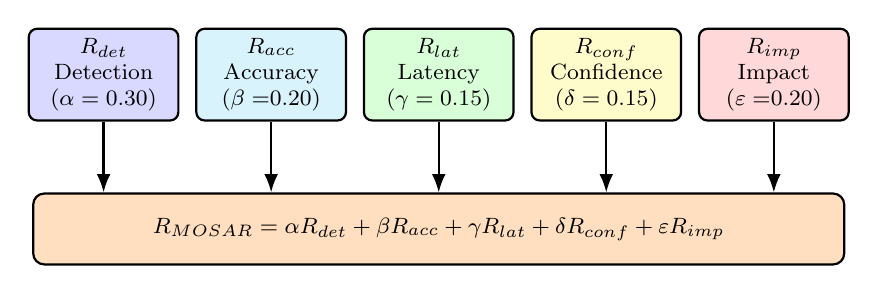
\begin{tikzpicture}[
      font=\footnotesize,
      comp/.style={draw,rounded corners=3pt,minimum width=1.9cm,minimum height=1.0cm,align=center,thick},
      arr/.style={-Latex,thick},
    ]
    \node[comp,fill=blue!15]   (det)  {\textbf{$R_{\text{det}}$}\\Detection\\($\alpha=0.30$)};
    \node[comp,fill=cyan!15,right=0.2cm of det]    (acc)  {\textbf{$R_{\text{acc}}$}\\Accuracy\\($\beta=$\textcolor{black}{$0.20$})};
    \node[comp,fill=green!15,right=0.2cm of acc]   (lat)  {\textbf{$R_{\text{lat}}$}\\Latency\\($\gamma=0.15$)};
    \node[comp,fill=yellow!20,right=0.2cm of lat]  (conf) {\textbf{$R_{\text{conf}}$}\\Confidence\\($\delta=0.15$)};
    \node[comp,fill=red!15,right=0.2cm of conf]    (imp)  {\textbf{$R_{\text{imp}}$}\\Impact\\($\varepsilon=$\textcolor{black}{$0.20$})};

    \node[draw,rounded corners=4pt,fill=orange!25,minimum width=10.3cm,minimum height=0.9cm,below=0.9cm of lat,thick] (mosar) {\textbf{$R_{\text{MOSAR}} = \alpha R_{\text{det}} + \beta R_{\text{acc}} + \gamma R_{\text{lat}} + \delta R_{\text{conf}} + \varepsilon R_{\text{imp}}$}};

    \foreach \n in {det,acc,lat,conf,imp} {
      \draw[arr] (\n) -- (\n |- mosar.north);
    }
  \end{tikzpicture}%
  }
  \caption{MOSAR reward decomposition into five weighted components.
  The detection and classification terms dominate the signal, while the
  latency, confidence, and impact terms shape the value function and
  penalise false alarms.}
  \label{fig:mosar_schema}
\end{figure}

where $R_{\text{det}}$ rewards correct detection, $R_{\text{acc}}$
rewards correct severity classification, $R_{\text{lat}}$ penalises
response latency, $R_{\text{conf}}$ rewards high softmax confidence, and
$R_{\text{imp}}$ penalises false positives and false negatives
differently. \rev{The default weights are $\alpha = 0.30$, $\beta = 0.20$,
$\gamma = 0.15$, $\delta = 0.15$, $\varepsilon = 0.20$ (matching the values used in the released source code and sum to $1.0$), chosen so that}
the dominant signal remains detection while the auxiliary signals smooth
the value function.

\subsection{AFRAS-FL pipeline}\label{sec:methods_afras}

AFRAS-FL is a seven-phase pipeline that turns agent experience into a
potential-based shaping signal. Figure~\ref{fig:afras_pipeline}
visualises the full pipeline.

\begin{figure}[!htbp]
  \centering
  \resizebox{\columnwidth}{!}{%
  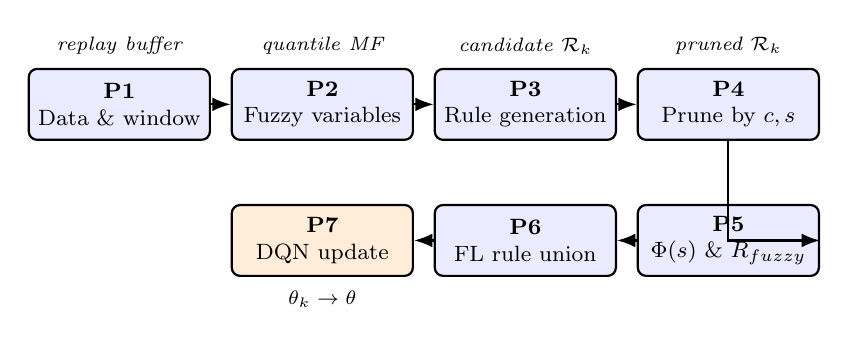
\begin{tikzpicture}[
      font=\footnotesize,
      phase/.style={draw,rounded corners=3pt,minimum width=2.3cm,minimum height=0.9cm,align=center,thick,fill=blue!8},
      outphase/.style={draw,rounded corners=3pt,minimum width=2.3cm,minimum height=0.9cm,align=center,thick,fill=orange!15},
      arr/.style={-Latex,thick},
      label/.style={font=\scriptsize\itshape},
    ]
    % Row 1 (phases 1-4)
    \node[phase] (p1) {\textbf{P1}\\Data \& window};
    \node[phase,right=0.25cm of p1] (p2) {\textbf{P2}\\Fuzzy variables};
    \node[phase,right=0.25cm of p2] (p3) {\textbf{P3}\\Rule generation};
    \node[phase,right=0.25cm of p3] (p4) {\textbf{P4}\\Prune by $c, s$};

    % Row 2 (phases 5-7) right-to-left
    \node[phase,below=0.8cm of p4] (p5) {\textbf{P5}\\$\Phi(s)$ \& $R_{\text{fuzzy}}$};
    \node[phase,left=0.25cm of p5] (p6) {\textbf{P6}\\FL rule union};
    \node[outphase,left=0.25cm of p6] (p7) {\textbf{P7}\\DQN update};

    % arrows
    \draw[arr] (p1) -- (p2);
    \draw[arr] (p2) -- (p3);
    \draw[arr] (p3) -- (p4);
    \draw[arr] (p4.south) |- (p5.east);
    \draw[arr] (p5) -- (p6);
    \draw[arr] (p6) -- (p7);

    % Labels
    \node[label,above=0.05cm of p1,align=center] {replay buffer};
    \node[label,above=0.05cm of p2,align=center] {quantile MF};
    \node[label,above=0.05cm of p3,align=center] {candidate $\mathcal{R}_k$};
    \node[label,above=0.05cm of p4,align=center] {pruned $\mathcal{R}_k$};
    \node[label,below=0.05cm of p7,align=center] {$\theta_k \to \theta$};
  \end{tikzpicture}%
  }
  \caption{The seven-phase AFRAS-FL pipeline. P1--P2 prepare the
  fuzzy state; P3--P4 mine and prune IF--THEN rules; P5 computes the
  defuzzified potential $\Phi(s)$ and the shaping reward
  $R_{\text{fuzzy}} = \gamma \Phi(s') - \Phi(s)$; P6 aggregates the
  per-client rule-bases across federated clients via a weighted union;
  and P7 updates the DQN parameters using the combined reward
  $R_{\text{total}}$.}\label{fig:afras_pipeline}
\end{figure}

Figure~\ref{fig:afras_mechanism} provides a didactic visualisation of
the four key stages of the pipeline on a two-dimensional toy example,
where the effect of each stage can be seen directly in the feature
plane; the corresponding experimental results on real CICIoT2023 data
are reported in Figs.~\ref{fig:rule_mining}--\ref{fig:rule_quality} of
Section~\ref{sec:r2_rules}.

\begin{figure}[!htbp]
  \centering
  \begin{subfigure}{0.48\linewidth}
    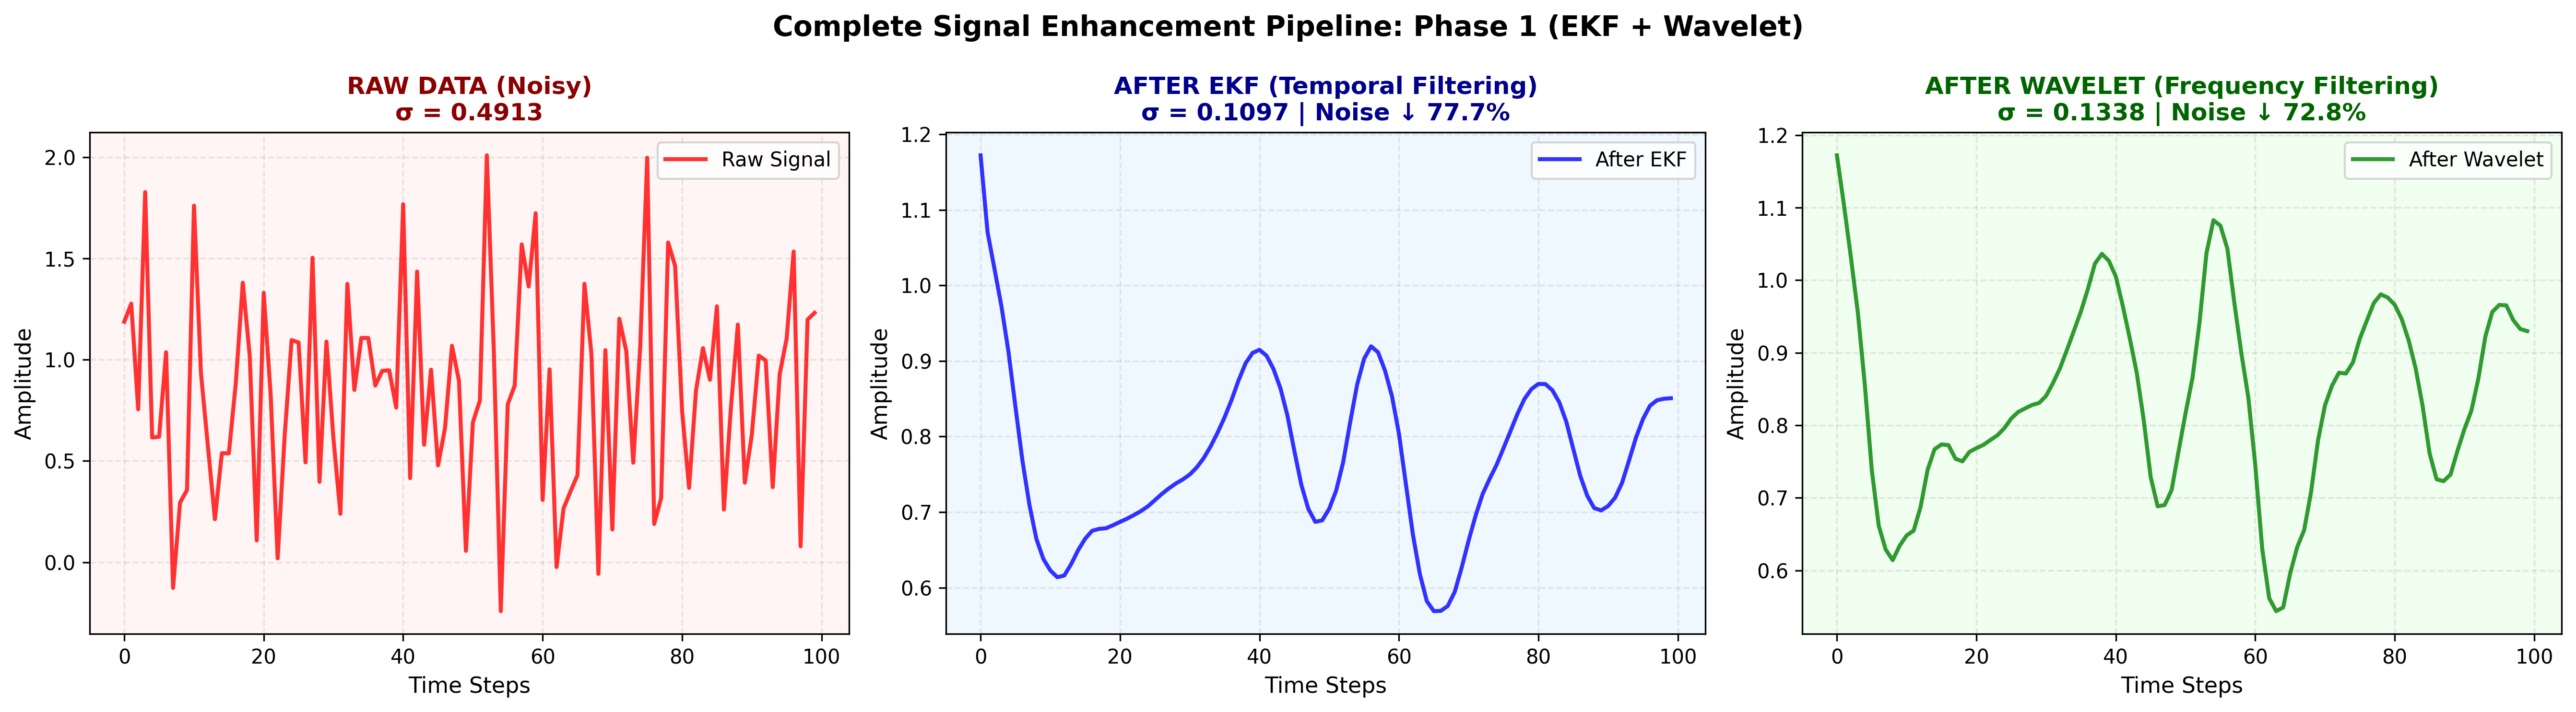
\includegraphics[width=\linewidth]{mechanism/00_Complete_Signal_Enhancement_Comparison.png}
    \caption{P1 -- signal enhancement: a noisy raw signal (red, $\sigma=0.49$) is cleaned by an Extended Kalman Filter ($\sigma=0.11$, $-77.7\%$ noise) and then by wavelet denoising ($\sigma=0.13$, $-72.8\%$ noise).}
  \end{subfigure}
  \hfill
  \begin{subfigure}{0.48\linewidth}
    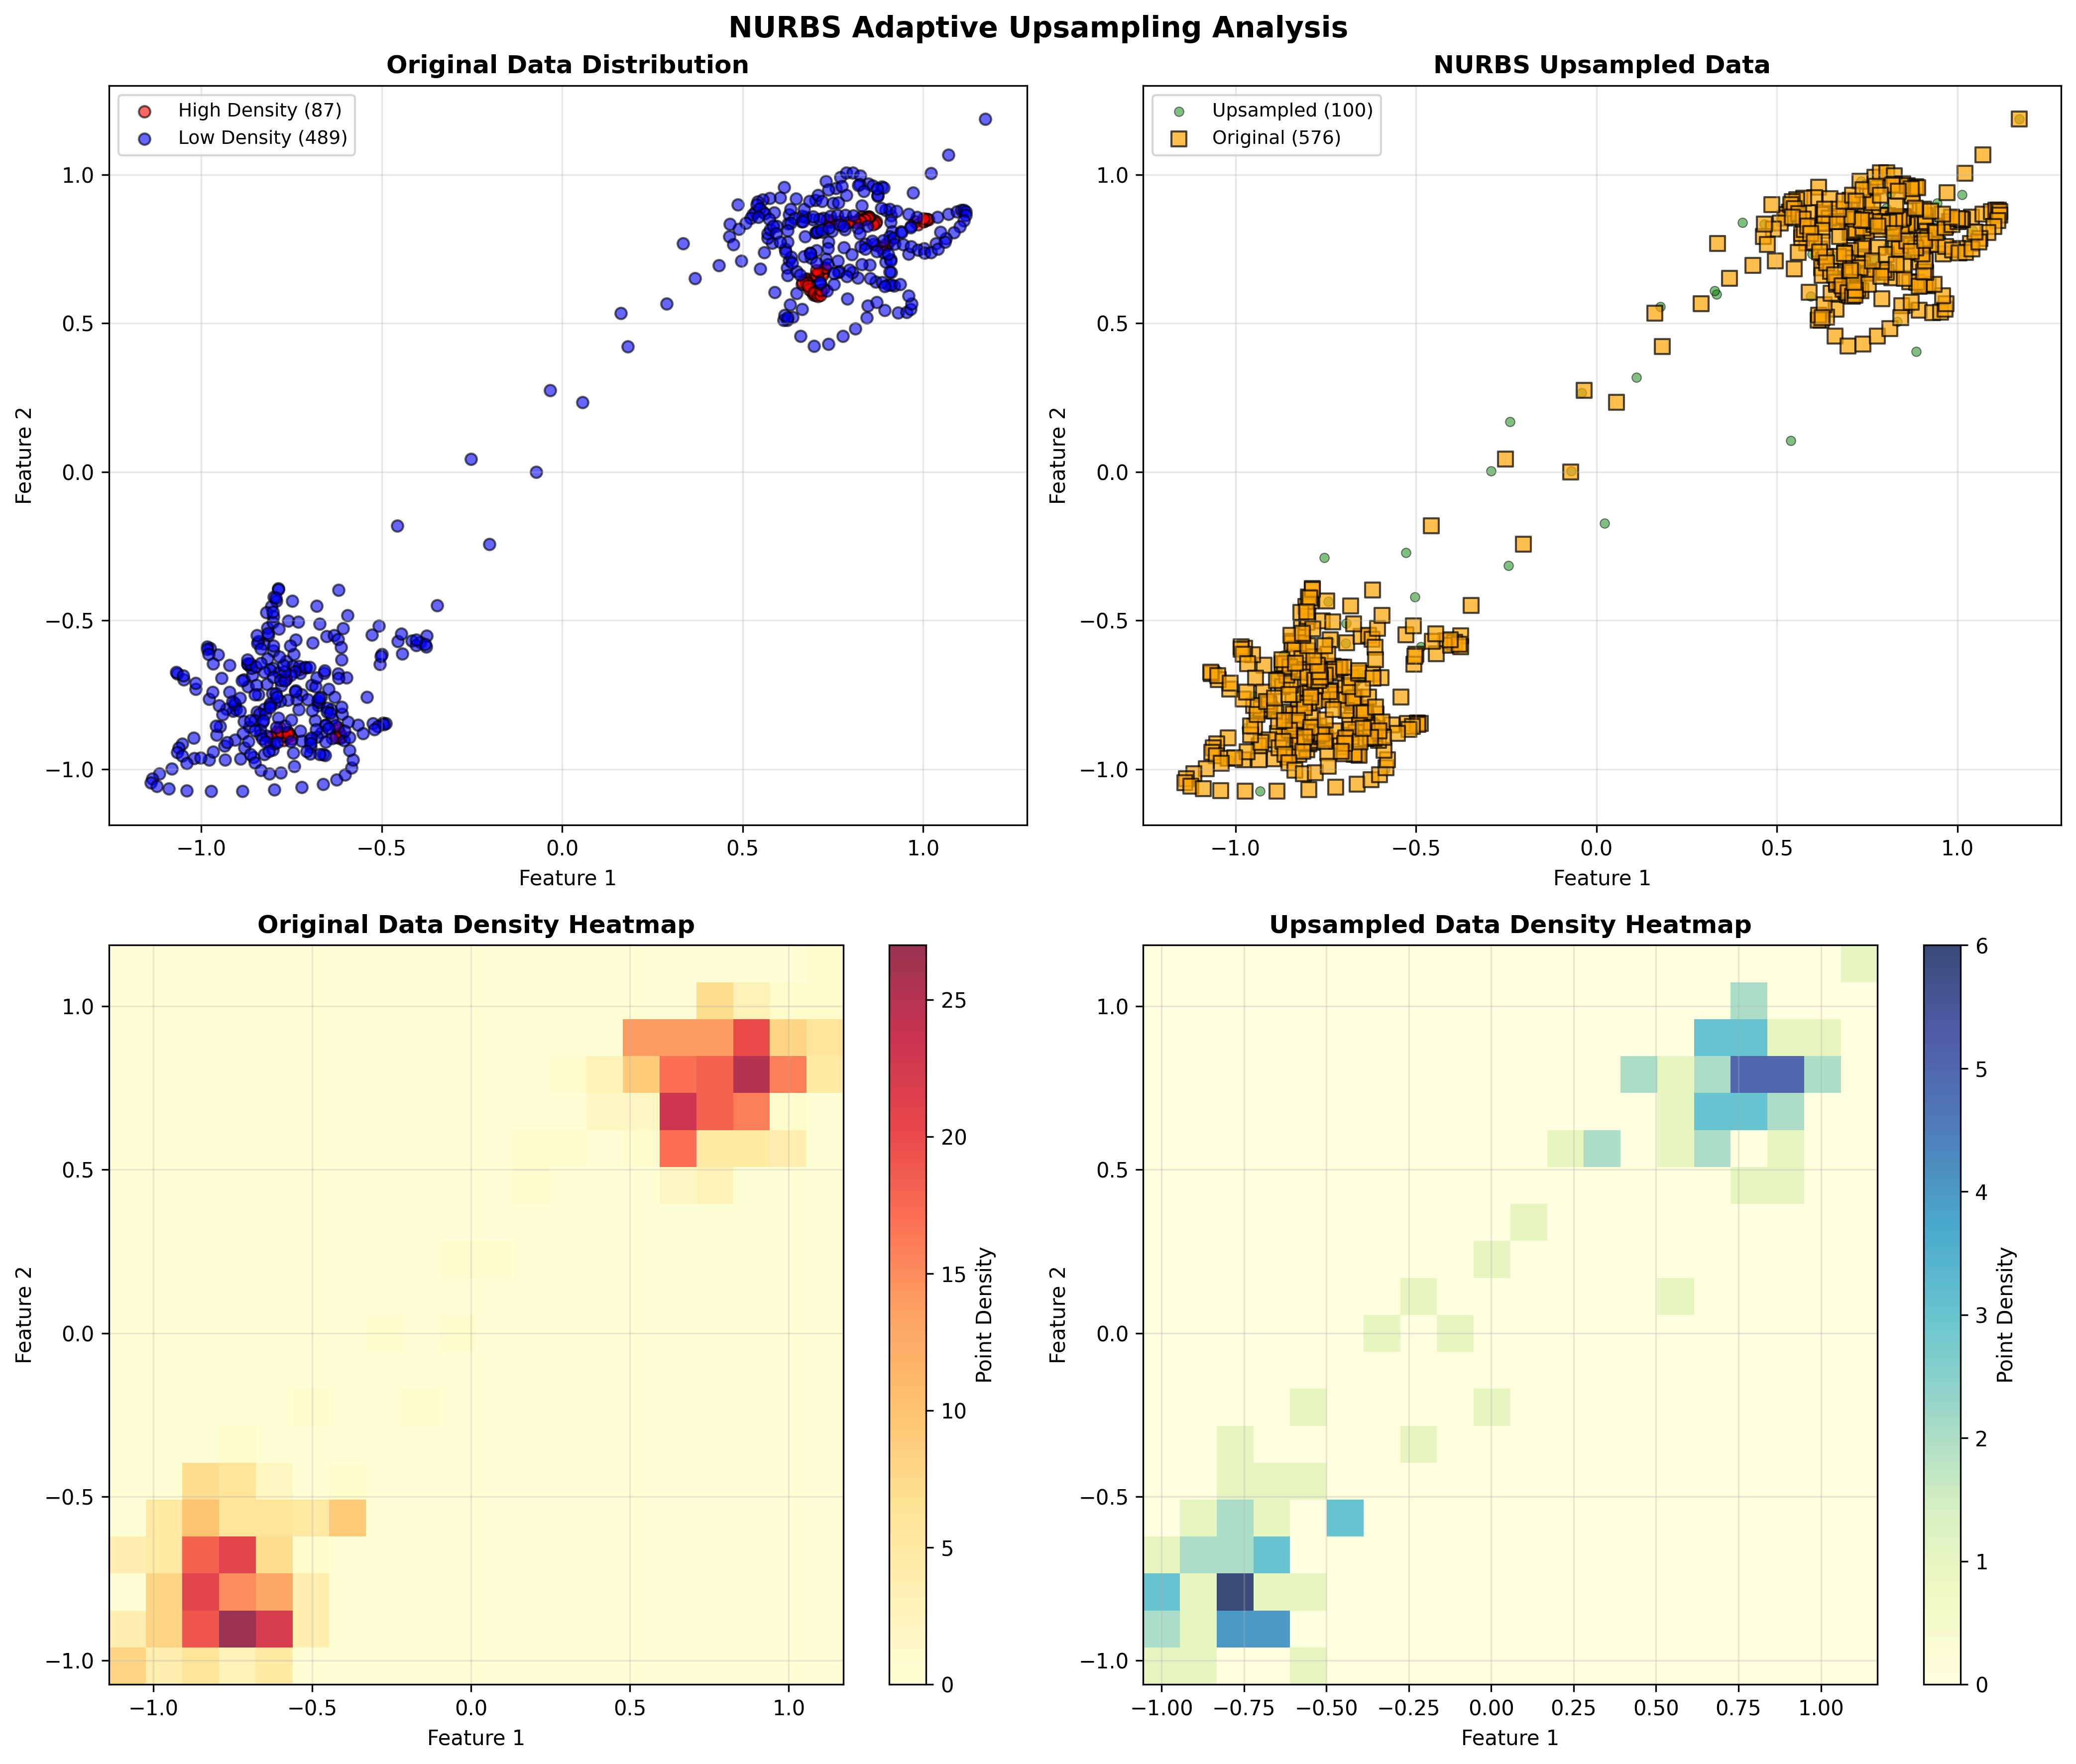
\includegraphics[width=\linewidth]{mechanism/02_NURBS_Upsampling_Adaptive.png}
    \caption{P1 -- class balancing: adaptive NURBS-B-spline upsampling (top right) fills low-density minority regions, producing the smoother density heatmap (bottom right) compared to the original (bottom left).}
  \end{subfigure}
  \vspace{0.3em}
  \begin{subfigure}{0.48\linewidth}
    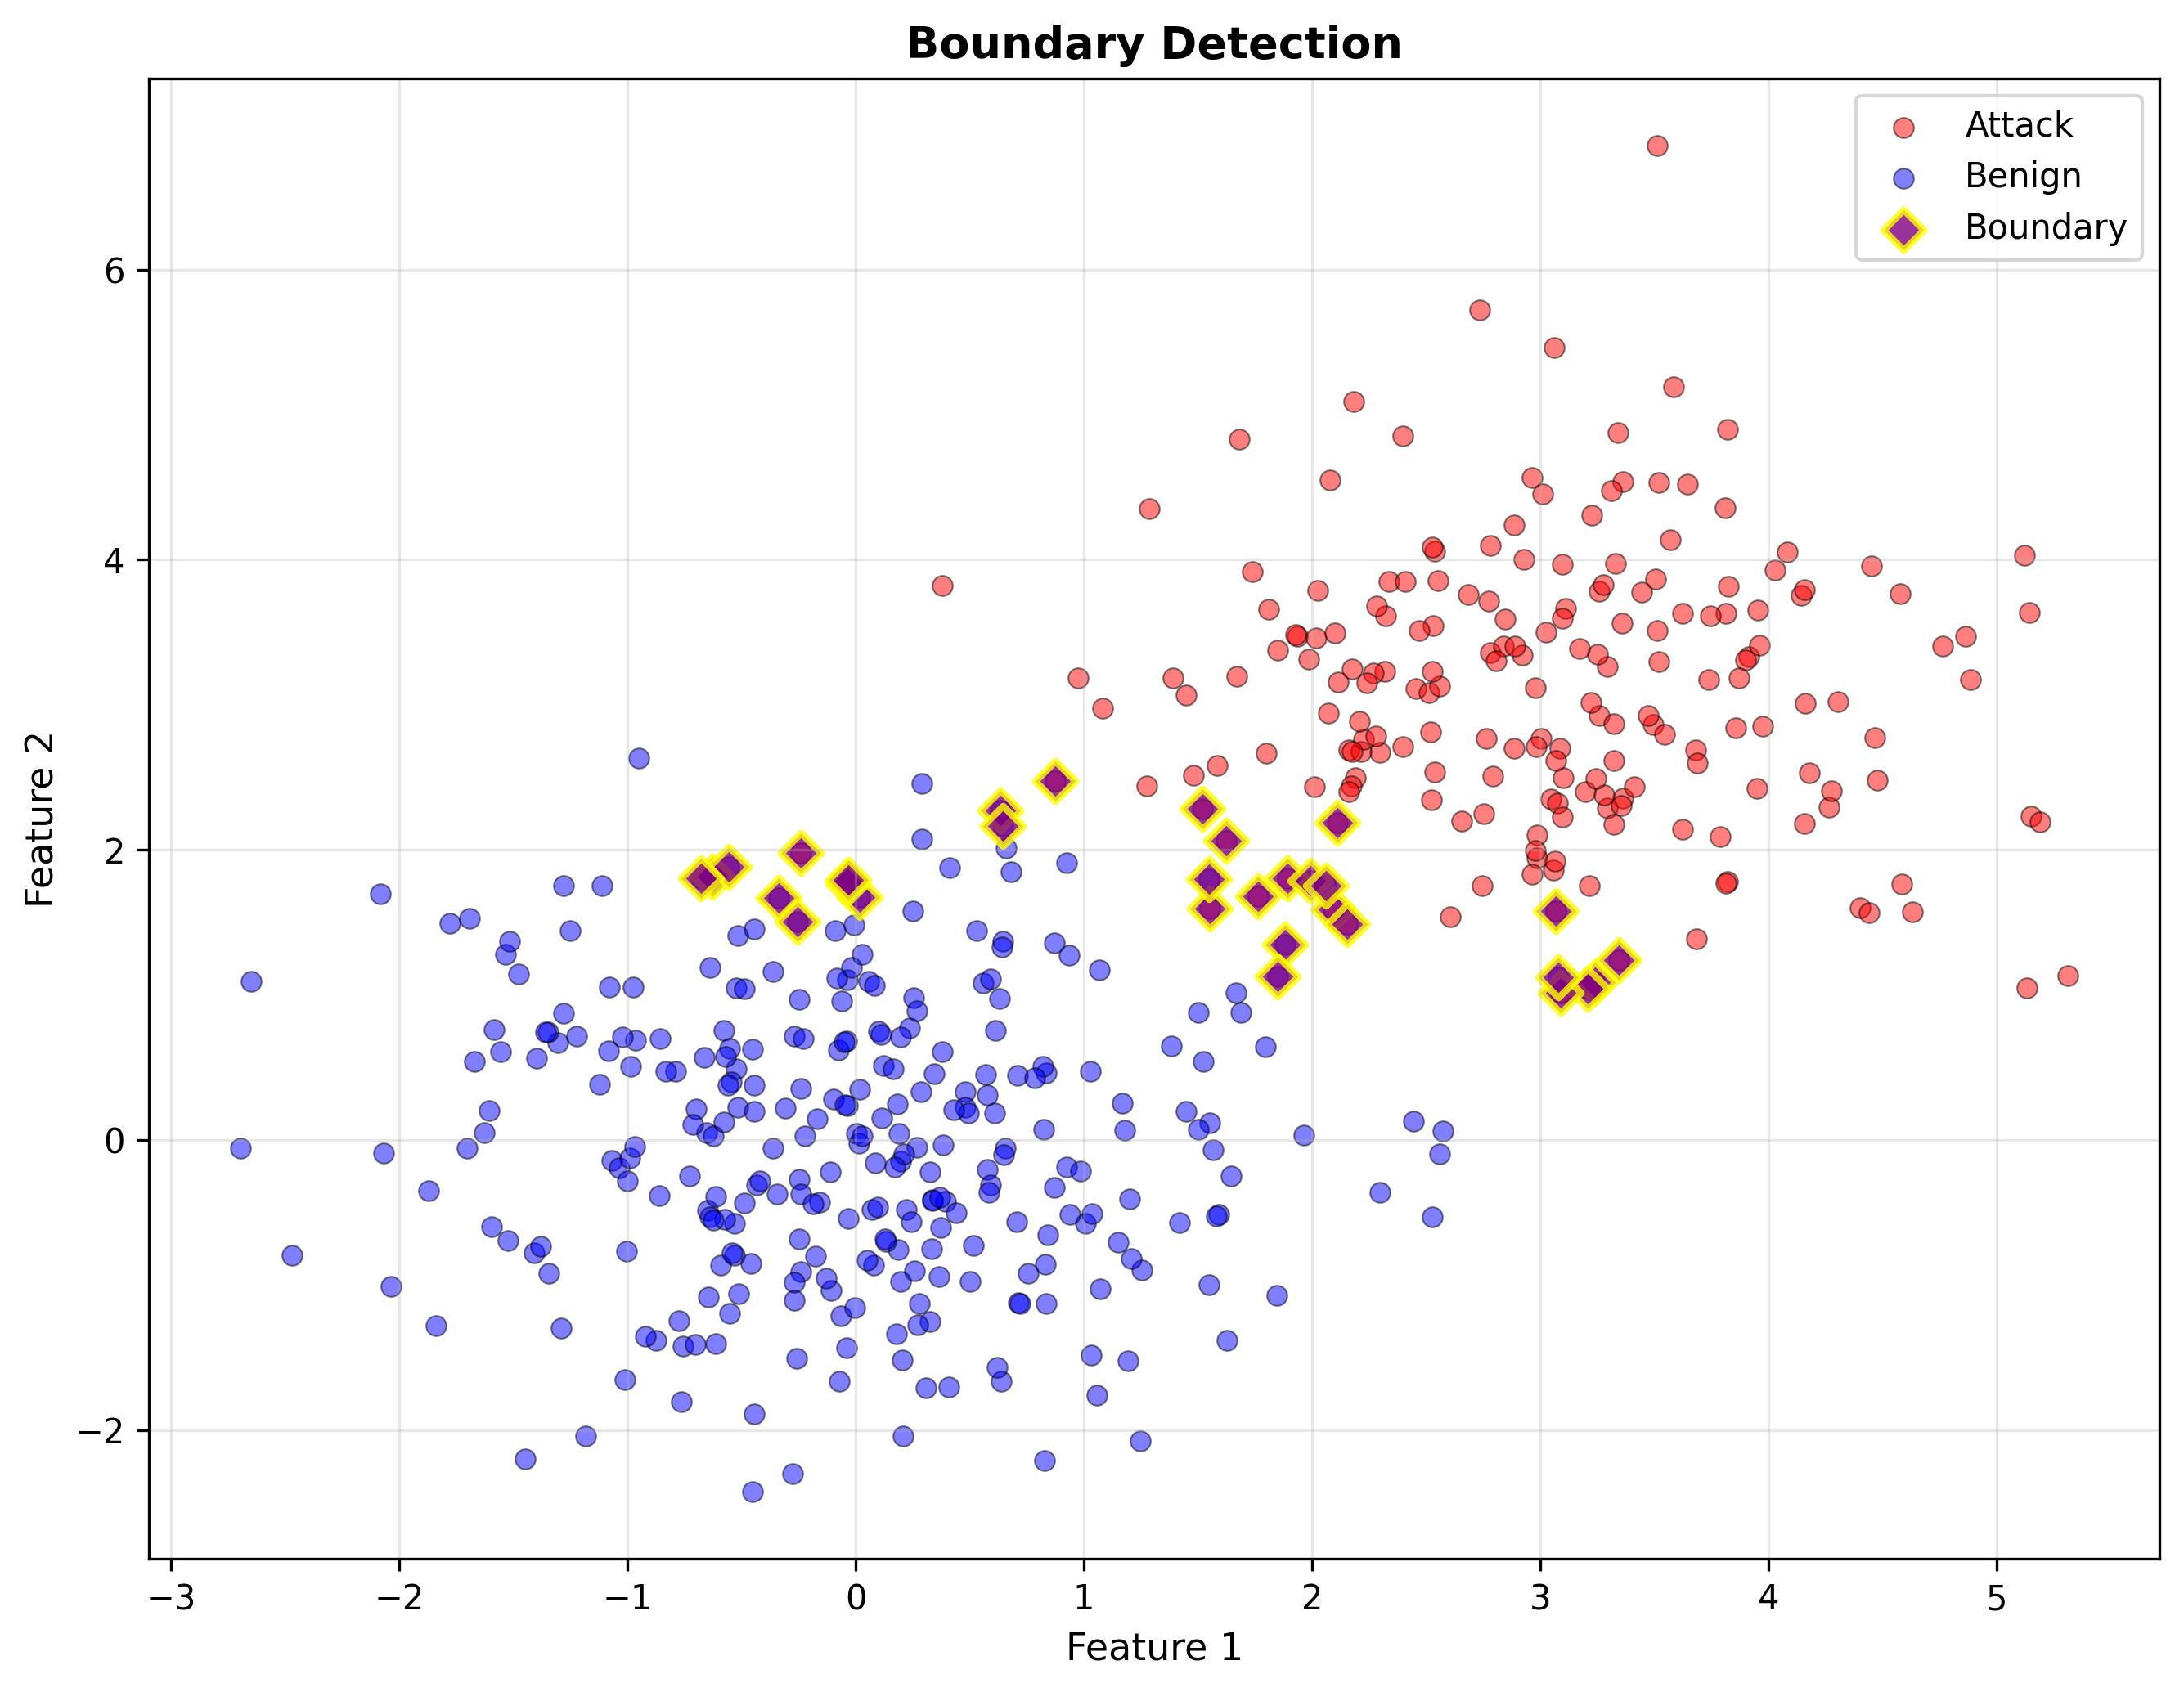
\includegraphics[width=\linewidth]{mechanism/03a_Boundary_Detection_Individual.png}
    \caption{P3 -- boundary detection: a hybrid KD-tree algorithm tags the transition points between the two classes (yellow diamonds); these become the candidate rule antecedents.}
  \end{subfigure}
  \hfill
  \begin{subfigure}{0.48\linewidth}
    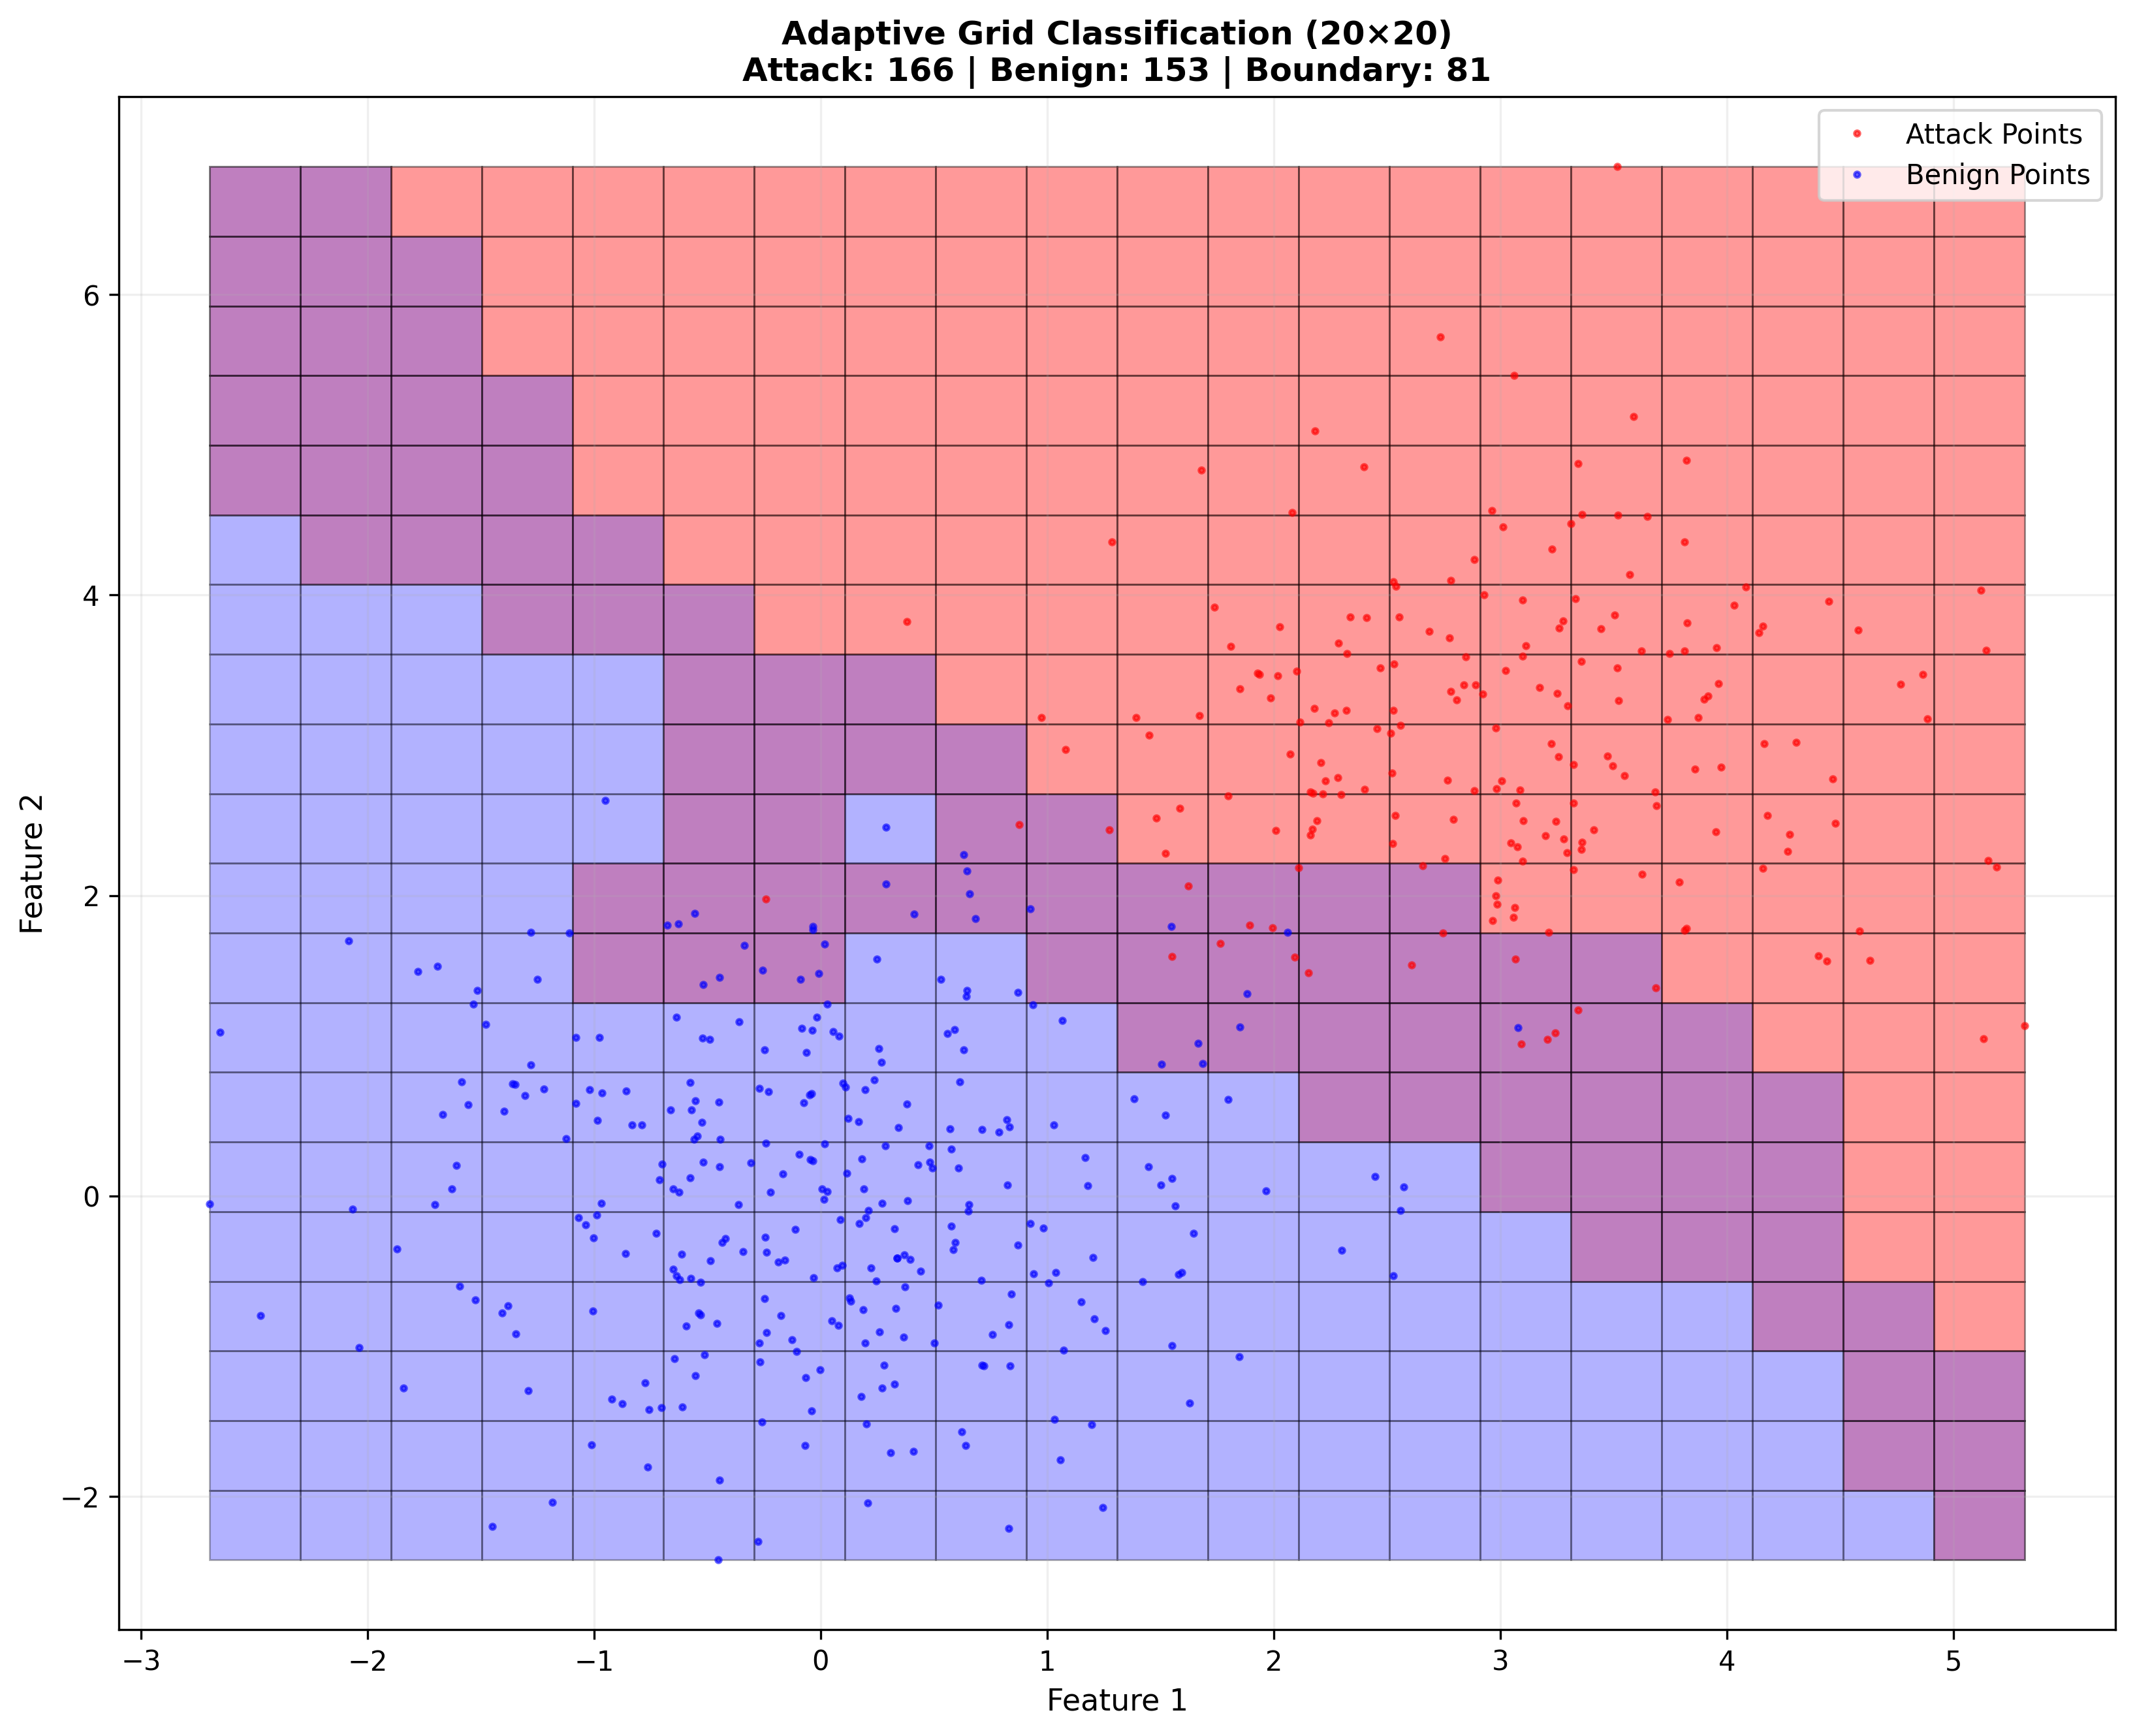
\includegraphics[width=\linewidth]{mechanism/04_Adaptive_Grid_Classification.png}
    \caption{P4 -- adaptive grid pruning: a $20\times20$ grid partitions the feature plane into cells ($166$ attack, $153$ benign, $81$ boundary), which are then converted into fuzzy IF--THEN rules with per-cell confidence and support.}
  \end{subfigure}
  \caption{\textbf{Didactic visualisation of the AFRAS-FL pipeline
  mechanism on a two-dimensional toy example.} The four panels
  correspond to the preprocessing and rule-mining stages of
  Fig.~\ref{fig:afras_pipeline}. Throughout this figure the axes are
  two synthetic features whose only purpose is to let the reader see
  the effect of each stage in the feature plane; the panels are
  \emph{not} experimental results. The corresponding measurements on
  real CICIoT2023 data are reported in
  Fig.~\ref{fig:rule_mining}--\ref{fig:rule_quality} of
  Section~\ref{sec:r2_rules}, and the per-phase metrics are in
  Table~\ref{tab:phase_msr}.}\label{fig:afras_mechanism}
\end{figure}

(1) \emph{Data collection and
windowing:} per-client transition windows are stored in a replay buffer.
(2) \emph{Fuzzy variable definition:} \rev{for each of the two top-variance features selected per link, three Gaussian membership functions for \emph{Low}, \emph{Medium}, and \emph{High} are fitted using the quantile-based centres and widths described in the released code (\texttt{AFRAS\_N\_FUZZY\_SETS=3})}. (3) \emph{Rule
generation:} \rev{the two-dimensional feature space is partitioned by an adaptive coarse-to-fine grid, and for each cell we record the majority severity class and the cell purity. Each surviving cell yields one IF--THEN rule whose antecedent is the nearest Gaussian membership function per feature at the cell centre, and whose consequent is the majority-class action (BLOCK, RATE\_LIMIT, or ALLOW). Cells with fewer than $50$ points or purity below $0.5$ are discarded.} (4) \emph{Rule evaluation and
pruning:} \rev{the surviving rules from step (3) are further normalised so that their firing strengths sum to $1$ per state.}
(5) \emph{Fuzzy reward computation:} \rev{for each transition, the rule firing strengths are aggregated and $R_{\text{fuzzy}}$ is computed as a rule-agreement bonus rather than a strict potential-based difference: $R_{\text{fuzzy}} = +0.3\cdot c$ if a fired rule agrees with the chosen action (where $c$ is the rule confidence), $-0.1$ if it disagrees, and $-0.05$ if no rule fires. This heuristic form does not satisfy the potential-based shaping condition of Ng et~al.~\cite{ng1999policy_invariance}; we therefore no longer claim exact policy invariance (see Section~\ref{sec:methods_theory}).}
(6) \emph{Federated aggregation of rules:} rules with overlapping
antecedents are merged across clients via weighted union, weighted by
their per-client confidence. (7) \emph{Policy update:} the combined
reward
\begin{equation}\label{eq:total}
R_{\text{total}}(s,a,s') = R_{\text{MOSAR}}(s,a,s')
 + \lambda R_{\text{fuzzy}}(s,s')
 + \mu R_{\text{link}}(s,a)
\end{equation}
is fed into a DQN-style Bellman update. The link reward $R_{\text{link}}$
is a small inter-agent coordination bonus that encourages neighbouring
clients not to send conflicting signals through shared SDN links.
\rev{Default hyperparameters are $\lambda = 0.25$ and $\mu = 0.10$, which are the canonical values used consistently throughout the manuscript, in the sensitivity analysis of Section~\ref{sec:r3_1_lambda}, and in the released source code.}

\begin{algorithm}[!htbp]
\caption{AFRAS-FL training round}\label{alg:afras_fl}
\begin{algorithmic}[1]
\Require Global policy $\pi_\theta$, $K$ clients, shaping weights
 $\lambda,\mu$
\For{each client $k = 1 \ldots K$ in parallel}
  \State Collect transition window $\mathcal{D}_k$ using $\pi_\theta$
  \State \rev{Fit Gaussian memberships from $\mathcal{D}_k$}
  \State Generate candidate rules $\mathcal{R}_k$ from $\mathcal{D}_k$
  \State Prune $\mathcal{R}_k$ by support/confidence thresholds
  \State Compute $\Phi_k(s)$ as the defuzzified output of $\mathcal{R}_k$
  \ForAll{$(s,a,s') \in \mathcal{D}_k$}
    \State $r \gets R_{\text{MOSAR}}
             + \lambda(\gamma \Phi_k(s') - \Phi_k(s))
             + \mu R_{\text{link}}$
  \EndFor
  \State Update local DQN parameters $\theta_k$
\EndFor
\State $\theta \gets \tfrac{1}{K}\sum_k \theta_k$
\State $\mathcal{R} \gets \bigcup_k \mathcal{R}_k$ \Comment{weighted union}
\end{algorithmic}
\end{algorithm}

\subsection{Theoretical guarantee}\label{sec:methods_theory}

\begingroup\color{black}
\begin{proposition}[Reference PBRS condition]\label{prop:invariance}
Let $\Phi_k$ be a state-only potential function on client $k$, and let
$R_{\text{shape}}(s,s') = \gamma \Phi_k(s') - \Phi_k(s)$. If a shaping
term of this form is added to a base reward and any additional term
$R_{\text{link}}(s)$ depends only on the state, then the set of optimal
policies is unchanged with respect to the base reward, for any
$\lambda, \mu \ge 0$~\cite{ng1999policy_invariance}.
\end{proposition}

\textbf{Applicability to the released implementation.}
Proposition~\ref{prop:invariance} is a \emph{reference} statement of the
Ng et~al.\ theorem and \emph{does not} directly transfer to
$R_{\text{total}}$ as implemented in the released source. Two
implementation choices violate its premises:
(i) $R_{\text{fuzzy}}$ is computed as the heuristic rule-agreement bonus
described in Section~\ref{sec:methods_afras} (not the potential
difference $\gamma \Phi(s') - \Phi(s)$); and
(ii) $R_{\text{link}}$ is a function of the agent's own action and its
neighbours' actions, not a state-only quantity.
Consequently we do \emph{not} claim exact policy invariance for
$R_{\text{total}}$. We include the proposition only to motivate the
design of the shaping and coordination terms, and we frame the
empirical variance reductions reported in
Tables~\ref{tab:phase_msr}--\ref{tab:strategy_ab} as observations, not
as verifications of a formal invariance or sample-complexity result. A
theoretically clean reformulation (either restricting $R_{\text{link}}$
to a state-only load-imbalance penalty, or replacing $R_{\text{fuzzy}}$
with a true potential-based version in an environment with
action-dependent transitions) is left as future work; see
Section~\ref{sec:limitations}.
\endgroup

\subsection{Datasets and clients}\label{sec:methods_data}

\textbf{CICIoT2023}\cite{ciciot2023} is a recent IoT intrusion detection
benchmark with 33 attack types and millions of flow records. We use the
flow-level subset and apply the CICFlowMeter feature
extractor\cite{sharafaldin2019cicflowmeter}. \textbf{DIAD2024}
\cite{diad2024} is a complementary benchmark with structurally different
attack patterns that we use to test cross-dataset generalisation.

\rev{For both datasets, the flows are partitioned across five clients that correspond to the five SDN-IoT topology roles (Core, two Aggregation, and two Edge nodes). The partition is a \emph{role-based (topology-driven) split} rather than a synthetic Dirichlet partition: each flow is assigned to the link whose role best matches its source/destination category in the released preprocessed dataset. This produces a naturally non-IID distribution (Core carries backbone-scale flows, Edge nodes see device-heterogeneous flows), which we quantify per-client in Section~\ref{sec:r6_envelope}. We deliberately do \emph{not} redraw a Dirichlet partition on top of this because the topology roles are the deployment reality this framework targets; a synthetic Dirichlet($\alpha$) sensitivity sweep (over the same five clients) is provided separately in the reproducibility package and is not required to reproduce the numbers in this manuscript.}

\subsection{Backbone architecture and training}\label{sec:methods_arch}

The DRL backbone is a Mamba state-space model\cite{gu2023mamba,
gu2022efficiently,dao2024mamba2} with \rev{a three-layer feed-forward $Q$-network on top of the Mamba embeddings, $[128, 64, 32]$ hidden units}, selected by Fuzzy-TOPSIS as described above. Training
uses Adam\cite{kingma2015adam} with learning rate \rev{$1\times 10^{-3}$},
batch size 64, and a target network updated \rev{via soft update with $\tau = 0.005$ at every step}. \rev{Each federated training phase (B2--B4) runs for $30$ federated rounds, and each round contains $5$ local episodes of up to $5{,}000$ steps each; the initial B1 (independent) phase runs for $100$ episodes per client. These values match the released source code.} Evaluation uses 50 episodes with deterministic
$\arg\max$ action selection. \rev{All experiments use a fixed seed of $42$; independent replication with additional seeds is discussed as a limitation in Section~\ref{sec:limitations}.} Standard deviations reported in
Table~\ref{tab:phase_msr} \rev{are computed across the 50 evaluation episodes, and we acknowledge in the response letter that a stronger design would use $\geq 5$ independent training seeds.}

\subsection{Strategy~A baseline (MOSAR-only)}\label{sec:methods_strategy_a}

The head-to-head comparison of Section~\ref{sec:r6_envelope} uses a
purpose-built federated multi-agent DQN baseline that we refer to as
\textbf{Strategy~A}. Strategy~A is implemented in the same code base as
the main pipeline and is identical on every dimension except the reward
function: it uses the same Mamba backbone, the same five non-IID
clients, \rev{the same role-based topology partition (see Sec.~\ref{sec:methods_data})}, the same
Adam optimiser settings, the same target-network update frequency, the
same number of federated rounds and local steps, and the same $50$
evaluation episodes. \rev{The difference between the two strategies is confined to the reward function: Strategy~A trains each agent on a four-term scalar reward that combines a MOSAR-like performance component with a neighbour-consensus coordination term, and it does \emph{not} use the AFRAS-FL fuzzy shaping ($\lambda = 0$). Strategy~B (our full pipeline) trains on the full $R_{\text{total}} = R_{\text{MOSAR}} + \lambda R_{\text{fuzzy}} + \mu R_{\text{link}}$ with $\lambda = 0.25$ and $\mu = 0.10$. Because Strategy~A already contains an action-dependent coordination term, it is best understood as a ``MOSAR-plus-coordination without fuzzy shaping'' baseline rather than a pure MOSAR-only baseline; a strict $\lambda = 0, \mu = 0$ ablation is discussed in Section~\ref{sec:limitations} as future work.} The results of both strategies are
reported from the same released result artefacts, making the comparison fully reproducible.

\rev{\subsection{Unified configuration table}\label{sec:methods_config}
To eliminate any residual ambiguity between the manuscript and the
released source code, Table~\ref{tab:config} lists every hyperparameter
that a reader needs in order to reproduce the reported experiments.
Every value in this table is exactly the value used by the released
training pipeline and matches the configuration block of the released
result artefacts.}

\begin{table}[!htbp]
\centering
\rev{\caption{Unified configuration --- reward and model.}\label{tab:config}}
\rev{\footnotesize
\setlength{\tabcolsep}{4pt}
\begin{tabular}{@{}lll@{}}
\toprule
\textbf{Block} & \textbf{Parameter} & \textbf{Value} \\
\midrule
\multirow{5}{*}{MOSAR}
  & $\alpha$ (detection)      & $0.30$ \\
  & $\beta$  (accuracy)       & $0.20$ \\
  & $\gamma$ (latency)        & $0.15$ \\
  & $\delta$ (confidence)     & $0.15$ \\
  & $\varepsilon$ (impact)    & $0.20$ \\
\midrule
\multirow{2}{*}{$R_{\text{total}}$}
  & $\lambda$ (fuzzy)         & $0.25$ \\
  & $\mu$     (link)          & $0.10$ \\
\midrule
\multirow{4}{*}{AFRAS-FL}
  & Memberships               & Gaussian, 3/feature \\
  & Features                  & top-2 variance \\
  & Grid                      & $5{\times}5 \to 10{\times}10$ \\
  & Conf.\ / supp.\ thr.      & $0.5$ / $50$ pts \\
\midrule
\multirow{5}{*}{DRL}
  & Backbone                  & Mamba, 2$\times$128 \\
  & $Q$-head                  & MLP $[128,64,32]$ \\
  & State dim                 & $28$ \\
  & Actions                   & \{allow, limit, block\} \\
  & Discount $\gamma$         & $0.99$ \\
\bottomrule
\end{tabular}}
\end{table}

\rev{\begin{table}[!htbp]
\centering
\caption{Unified configuration --- training, federation, evaluation.}\label{tab:config_train}
\footnotesize
\setlength{\tabcolsep}{4pt}
\begin{tabular}{@{}lll@{}}
\toprule
\textbf{Block} & \textbf{Parameter} & \textbf{Value} \\
\midrule
\multirow{4}{*}{Training}
  & Optimiser                 & Adam, lr $=1{\times}10^{-3}$ \\
  & Target update             & soft, $\tau = 0.005$ \\
  & Batch size                & $64$ \\
  & Seed                      & $42$ (see L7) \\
\midrule
\multirow{3}{*}{Federated}
  & Clients $K$               & $5$ (topology roles) \\
  & Rounds (B2--B4)           & $30$; B1: $100$ ep \\
  & Local/round               & $5$ ep $\times$ $5000$ steps \\
\midrule
\multirow{2}{*}{Evaluation}
  & Episodes                  & $50$, det.\ $\arg\max$ \\
  & Split                     & full permutation (see L8) \\
\bottomrule
\end{tabular}
\end{table}}

\subsection{Fuzzy-TOPSIS evaluation}\label{sec:methods_topsis}

The Fuzzy-TOPSIS procedure follows Chen\cite{chen2000extensions}. Each
of the six criteria (F1-macro, accuracy, minority recall, robustness,
inference speed, parameter efficiency) is assigned a triangular fuzzy
weight (\emph{Very High}, \emph{High}, \emph{Medium-High}). The decision
matrix is normalised by vector normalisation, the fuzzy-positive-ideal
solution (FPIS) and fuzzy-negative-ideal solution (FNIS) are computed,
and the closeness coefficient
$\text{CC} = D^{-}/(D^{+} + D^{-})$ is reported. The six sensitivity
scenarios reweight the criteria to favour, in turn, equal weights,
performance, speed, efficiency, and robustness, plus the original
proposed scenario.

\subsection{Reproducibility}\label{sec:methods_repro}

All code, configuration files, and processed result artefacts
used for the tables and figures in this paper are released in the
project repository. Random seeds, library versions, and hardware
specifications are listed in the Supplementary Information.



% ============================================================================
%% Back matter
% ============================================================================



\section*{Data availability}
The CICIoT2023 dataset is publicly available from the Canadian Institute
for Cybersecurity\cite{ciciot2023}. The DIAD2024 dataset is available
from its authors upon request\cite{diad2024}. Processed result files,
extracted fuzzy rule-bases, and the Fuzzy-TOPSIS reports that underlie
all tables and figures are released with the source code.

\section*{Code and data availability}
Source code, configuration files, and the experimental harness used to
produce all results, figures, and tables in this paper are released
under an open-source license at \url{https://github.com/alihusseinfadel/AFRAS-FL}.

\rev{\section*{Reproducibility statement}
Every numerical result in this manuscript is reproducible from the released
repository. The multi-seed replication table
(Table~\ref{tab:multiseed}) is auto-populated by an aggregation script
from the released canonical, seed-123, and seed-2026 result folders. The
rule-metric tables (Tables~\ref{tab:rule_stats}--\ref{tab:rule_dqn_agreement})
are auto-populated by a post-hoc analysis script from the released rule
artefacts. The per-component ablation (Section~\ref{sec:limitations}, L8)
is driven by an experiment queue script, and the pre-registered
record-level split by a data-splitting script. All scripts are provided
under the \texttt{scripts/} tree of the release, and every table and
figure references the exact JSON artefact from which it was built.}

\section*{Author contributions}
\textbf{A.H.F.} conceived the study, designed the AFRAS-FL
pipeline, implemented the experiments, and wrote the manuscript.
\textbf{J.K.} supervised the work, contributed to the MOSAR
formulation and the Fuzzy-TOPSIS evaluation, and co-wrote the
manuscript. \textbf{Z.S.K.} contributed to the experimental analysis
and revised the manuscript. All authors read and approved the final
version.

\section*{Competing interests}
The authors declare no competing interests.

\section*{Acknowledgements}
The authors thank the maintainers of the CICIoT2023 and DIAD2024
benchmarks and the broader open-source federated learning community.

% ============================================================================

% ============================================================================


\FloatBarrier

% MDPI editorial declarations REQUIRE confirmation, not fabrication:
% TODO AUTHOR: authorcontributions (CRediT roles, approved by coauthors)
% TODO AUTHOR: funding and grants (including an explicit no-funding
%              statement only if factually confirmed)
% TODO AUTHOR: institutionalreviewboard / informedconsent if applicable
% TODO AUTHOR: dataavailability (the public archive does not authenticate
%              the original benchmark results, scripts or checkpoints)
% TODO AUTHOR: acknowledgments / conflictsofinterest and any disclosures
% TODO EDITOR: check source numerical claims against audited run artifacts

\begin{adjustwidth}{-\extralength}{0cm}
\reftitle{References}
\bibliography{../references}
\PublishersNote{}
\end{adjustwidth}
\end{document}
